\documentclass{purcell}

%% BEGIN TITLE

\makeindex

\makeatletter
\def\maketitle{%
  \null
  \thispagestyle{empty}%
  \vfill
  \begin{center}\leavevmode
    \normalfont
    {\LARGE\raggedleft \@author\par}%
    \hrulefill\par
    {\huge\raggedright \@title\par}%
    \vskip 1cm
%    {\Large \@date\par}%
  \end{center}%
  \vfill
  \null
  \cleardoublepage
  }
\makeatother
\author{Edward M.~Purcell}
\title{Electricity and Magnetism}

\begin{document}

\let\cleardoublepage\clearpage


\maketitle






\frontmatter

\null\vfill

\begin{flushleft}
\textit{Electricity and Magnetism}


Copyright (c) 1963, 1964, 1965 by Education Development Center, Inc., \url{edc.org}.

The following notices are reproduced from the 1965 edition of the book:\\
``The preparation of this course was supported by a grant from the National Science
Foundation to Educational Services Incorporated.''\\
``In accordance with the National Science Foundation's policies concerning curriculum revision material
developed under their auspices, McGraw-Hill Book Company, a division of McGraw-Hill, Inc.,
announces that the material in the Berkeley Physics Course, Vol. II ELECTRICITY AND MAGNETISM,
which is copyrighted by Education Development Center (a successor by merger to Educational
Services, Inc.) and published by McGaw-Hill Book Company in 1965, will be available for use
by authors and publishers on a royalty-free basis on or after April 30, 1970. Interested
parties should address inquiries to the Managing Director, Educational Development Center,
55 Chapel Street, Newton, Massachusetts, 02160.''

Copyright (c) 2013 by Benjamin Crowell and others as named in log files. All contributors have
agreed that the work involved in producing a verbatim reproduction of the 1965 edition is to be
released under the Creative Commons CC0 license, \url{http://creativecommons.org/publicdomain/zero/1.0/}.

\end{flushleft}
\let\cleardoublepage\clearpage

\pagebreak

\tableofcontents

\mainmatter
\addtocounter{page}{5}
\sloppy

\chapter{Electrostatics: charges and fields}

\section{Electric charge}\index{charge}

Electricity appeared to its early investigators as an extraordinary phenomenon.
To draw from bodies the \emph{subtle fire}, as it was
sometimes called, to bring an object into a highly electrified state, to
produce a steady flow of current, called for skillful contrivance. Except for
the spectacle of lightning, the ordinary manifestations of nature, from the
freezing of water to the growth of a tree, seemed to have no relation to the
curious behavior of electrified objects. We know now that electrical forces
largely determine the physical and chemical properties of matter over the whole
range from atom to living cell. For this understanding we have to thank the
scientists of the nineteenth century, Ampere, Faraday, Maxwell, and many
others, who discovered the nature of electromagnetism,, as well as the
physicists and chemist of the twentieth century who unraveled the atomic
structure of matter. 

Classical electromagnetism deals with electric charges and
currents and their interactions as if all the quantities involved could be
measured independently, with unlimited precision. Here \emph{classical} means
simply ``non-quantum.'' The quantum law with its constant $h$ is ignored in the
classical theory of electromagnetism, just as it is in ordinary mechanics. Indeed,
the classical theory was brought very nearly to its present state of completion
before Planck's discovery. It has survived remarkably well. Neither the
revolution of quantum physics nor the development of special relativity dimmed
the luster of the electromagnetic field equations Maxwell wrote down a hundred
years ago. 

Of course, the theory was solidly based on experiment, and
because of that was fairly secure within its original range of application --to
coils, capacitors, oscillating currents, eventually radio waves and light
waves. But even so great a success does not guarantee validity in another
domain, for instance, the inside of a molecule.

Two facts help explain the continuing importance in modern
physics of the classical description of electromagnetism. First, special
relativity required no revision of classical electromagnetism. Historically
speaking, special relativity \emph{grew out of} classical electromagnetic
theory and experiments inspired by it. Maxwell's field equations, developed
long before the work of Lorentz and Einstein, proved to be entirely compatible
with relativity. Second, quantum modifications of the electromagnetic force
have turned out to be unimportant down to distances less than $10^{-10}\ \textup{cm}$, a
hundred times smaller than the atom. We can describe the repulsion and
attraction of particles in the atom using the same laws that apply to the
leaves of an electroscope, although we need quantum mechanics to predict how
the particles will behave under those forces. For still smaller distances,
there is a rather successful fusion of electromagnetic theory and quantum
theory, called \emph{quantum electrodynamics}, which seems to agree with
experiment down to the smallest distances yet explored. 

We assume the reader has some acquaintance with elementary
facts of electricity. We are not going to review all the experiments by which
the existence of electric was demonstrated or all the evidence for the
electrical constitution of matter. On the other hand, we do want to look
carefully at the experimental foundations of the basic laws on which all else
depends. In this chapter we shall study the physics of stationary electric
charges --- \emph{electrostatics}.

Certainly one fundamental property of electric charge is its
existence I the two varieties that were long ago named positive and negative.
The observed fact is that all charged particles can be divided into two classes
such that all members of one class repel each other, while attracting members
of the other class. If two small electrically charged bodies $A$ and
$B$, some distance apart, repel one another, and if $A$ attracts some
third electrified body $C$, then we always find that $B$ attracts
$C$. Why this universal law prevails we cannot say for sure. But today
physicists tend to regard positive and negative charge as, fundamentally,
opposite manifestations of one quality, much as ``right'' and ``left'' are
opposite manifestations of ``handedness.'' Indeed, the question of symmetry
involved in right and left seems to be intimately related to this duality of
electric charge, and to another fundamental symmetry, the two directions of
time. Elementary particle physics is throwing some light on these questions.

What we call negative charge could just as well have been
called positive, and vice versa.\footnote{The charge of the ordinary electron has nothing
\emph{intrinsically negative} about it. A negative integer, once multiplication has been
defined, differs essentially from a positive integer in that its square is an integer of
opposite sign. But the product of two charges is not a charge; there is no comparison.}
The choice was a historical accident. Our
universe appears to be very evenly balanced mixture of positive and negative
electric charge which, since like charges repel one another is not surprising. 

Two other observed properties of electric charge are
essential in the electrical structure of matter: charge is conserved, and
charge is quantized. These properties involve \emph{quantity} of charge, and
thus imply a measurement of charge. Presently we shall state precisely how
charge can be measured in terms of the force between charges a certain distance
apart, and so on. But let us take this for granted, for the time being, so that
we may talk freely about these fundamental facts. 

\section{Conservation of charge}\index{charge!conservation of}\index{conservation!of charge}

The total charge in an isolated system never changes. By
\emph{isolated} we mean that no matter is allowed to cross the boundary of the
system. We could let light pass into or out of the system without affecting the
principle, since photons carry no charge. For instance, a thin-walled box in
vacuum, exposed to gamma rays, might become the scene of a ``pair-creation''
event in which a high-energy photon ends its existence with the creation of a
negative electron and a positive electron (Fig. 1.1). Two electrically charged
particles have been newly created but the net change in total charge, in and on
the box, is zero. An event that \emph{would} violate the law we have just
stated would be the creation of a positively charged particle \emph{without}
the simultaneous creation of a negatively charged particle. Such an occurrence
has never been observed. 

Of course, if the electric charges of electron and positron
were not precisely equal in magnitude, pair creation would still violate the
strict law of charge conservation. As well as can be determined from
experiment, their charges \emph{are} equal. An interesting experimental test is
provided by the structure called \emph{positronium}, a structure composed of an
electron and a positron, and nothing else. This curious ``atom'' can live long
enough-a tenth of a microsecond or so-to be studied in detail. It behaves as if
it were quite neutral, electrically. Actually, most physicists would be
astonished, not to say incredulous, if \emph{any} difference were found in the
magnitudes of these charges, for we know that electron and positron are related
to one another as \emph{particle} to \emph{antiparticle}. Their exact equality
of charge, like their equality of mass, is a manifestation of an apparently
universal symmetry in nature, the particle-antiparticle duality. One might
wonder whether charge conservation, then, is merely a corollary of some broader
conservation law governing the creation and annihilation of particles; or is
charge conservation a primary requirement, with which other laws have to fall
in line? Or do these questions make sense? We do not know for sure. 

One thing will become clear in the course of our study of
electromagnetism: nonconservation of charge would be quite incompatible with
the structure of our present electromagnetic theory. We may therefore state
either as a postulate of the theory or as an empirical law supported without
exception by all observations so far, the \emph{charge conservation law:}

The total electric charge in an isolated system, that is, the
algebraic sum of the positive and negative charge present at any time, never
changes. 

Sooner or later we must ask whether this law meets the test
of relativistic invariance. We shall postpone until Chap. 5 a thorough
discussion of this important question. But the answer is that it does, and not
merely in the sense that the statement above holds in any given inertial frame,
but in the stronger sense that observer in different frames, measuring the
charge, get the same number. In other words the total electric charge of an
isolated system is relativistically invariant number. 

\section{Quantization of charge}\index{charge!quantization of}\index{quantization of charge}

Millikan's oil-drop experiment,\index{Millikan oil drop experiment} and innumerable other
experiments, have shown that in nature electric charge comes in units of one
magnitude only. That magnitude we denote by $e$, the electronic charge. We have
already noted that the positron has precisely this amount of charge. What seems
more remarkable is the exact equality in the charges carried by all other
charged particles-the equality, for instance, in the magnitude of the positive
charge on the proton and the negative charge on the electron. 

That particular equality, the proton-electron charge
balance, is open to a very sensitive test. One can test the normal hydrogen
atom or molecule for overall electrical neutrality. Thus, one could try to
deflect a beam of atoms or molecules by an electrical field. In a sensitive
experiment devised for this purpose,\footnote{J.C.~Zorn, G.E.~Chamberlin,
and V.W.~Hughes, Phys. Rev. 129, 2566 (1963)} a sharply defined beam of cesium atoms was
sent, in a high vacuum, through a strong electric field. From the absence of
any observable deflection it could be concluded that the net charge on a cesium
atom must be less than $10^{-16}e$. An even more sensitive test has recently
been made by a different method.\footnote{J.G.~King, Phys. Rev. Letters 5, 562 (1960).
References to previous tests of charge equality will be found in this article and
in the chapter by V.W.~Hughes in Gravitation and Relativity, edited by H.Y.~Chiu and
W.F.~Hoffman (W.A.~Benjamin, Inc., New York, 1964), chap. 13.} A large amount of hydrogen gas was compressed
into a tank which was itself highly insulated, electrically, from its
surroundings. The gas was then allowed to escape from the tank by means which
prevented the escape of any ordinary ions. \emph{If} the charge on the proton
differed from that on the electron by, say, one part in a billion, then each
hydrogen molecule, composed of two protons and two electrons, would carry a
charge of $2\times 10^{-9}e$, and the departure of the whole mass of hydrogen would
measurably alter the electrical charge and potential of the tank. In fact, the
experiment could have revealed a residual charge as small as $10^{-20}e$ per
atom, and none was observed! We conclude that the electron and proton have
equal charge, to an accuracy of 1 part in $10^{20}$. 

On present ideas, the electron and the proton are about as
unlike as two elementary particles can be. No one yet understands why their
charges should have to be equal to such a fantastically precise degree.
Evidently the quantization of charge is a deep and universal law of nature.
\emph{All} charged elementary particles, as far as we can determine, carry
charges of precisely the same magnitude. We can only hope that some future
discovery or theoretical insight may reveal to us why a particle with a charge
$0.500e$, or $0.999e$, cannot exist.\footnote{In some recent theoretical speculations
about elementary particles the possible existence of charge $\frac{1}{3}e$ and $\frac{2}{3}e$
was suggested. In a subsequent search for such particles, under conditions believed
favorable for their production and detection, none turned up. [L.B.~Leipuner, W.T.~Chu,
R.C.~Larsen, R.K.~Adair, Particles with a charge of $\frac{1}{3}e$, Phys. Rev. Letters 12, 423 (1964)].
As this is written, however, the speculation continues.}

The fact of charge quantization lies outside the scope of
classical electromagnetism, of course. We shall usually ignore it, and act as
if our point charges $q$ could have any strength whatever. This will not get us
into trouble. Still, it is worth remembering that classical theory cannot be
expected to explain the structure of the elementary particles. (It is not
certain that present quantum theory can either!) What holds the electron
together is as mysterious as what fixes the precise value of its charge.
Something more than electrical forces must be involved, for the electrostatic
forces between different parts of the electron would be repulsive. 

In our study of electricity and magnetism we shall treat the
charged particles simply as carriers of charge, with dimensions so small
that

%%% ... partial sentence

\section{Flux}\index{flux}

The relation between the electric field and its sources can be
expressed in a remarkable simple way, one that we shall find very
useful. For this we need to define a quantity called \emph{flux}.

Consider some electric field in space and in this space some
arbitrary closed surface, like a balloon of any shape. Figure 1.13
shows such a surface, the field being suggested by a few field lines.
Now divide the whole surface into little patches which are so small
that over any on patch the surface is practically flat and the vector
field does not change appreciably from one part of a patch to
another. In other words, don't let the balloon be too crinkly, and
don't let its surface pass right through a singularity \footnote{By a
singularity of the field we would ordinarily mean not only a point
source where the field approaches infinity, but any place where the
field changes magnitude or direction discontinuously, such as an
infinitesimally thin layer of concentrated charge.
Actually this latter, milder, kind of singularity would cause no
difficulty here unless out balloon's surface were to coincide with
the surface of discontinuity over some finite area.} of the field
such as a point charge. The area of a patch defines a unique
direction ---the outward-pointing normal to its surface. (Since the
surface is closed you can tell its inside from its outside; there is
no ambiguity.) Let this magnitude and direction be represented by a
vector. Then for every patch into which the surface has been divided,
such as patch number $j$, we have a vector $\vc{a}_j$, giving its area
and orientation. The steps we have just taken are pictured in Fig.
1.13b and c. Note the vector $\vc{a}_j$ does not depend at all on
the shape of the patch; it doesn't matter how we have divided up the
surface, as long as the patches are small enough.

Let $\vc{E}_j$ be the electric field vector at the location of patch
number $j$. The scalar product $\vc{E}_j \cdot a_j$ is a number.
We call this number the \emph{flux} through that bit of surface.
To understand the origin of the same name, imagine a vector function
which represents the velocity of motion in a fluid ---say in a river,
where the velocity varies from one place to another but is constant
in time at any one position. Denote this vector field by $v$,
measured, say, in feet per second. Then if $a$ is the oriented area,
in square feed, of a frame lowered into the water, $\vc{v} \cdot \vc{a}$
is the \emph{rate of flow} of water through the fame in cubic feet
per second (Fig. 1.14). We must emphasize that our definition of
flux is applicable to any vector function, whatever physical variable
it may represent.

Now let us add up all the flux through all the patches to get the
flux through the entire surface, a scalar quantity which we shall
denote by $\Phi$:
\begin{equation} 
  \Phi= \sum\limits_{\text{All}~j}\vc{E}_j \cdot \vc{a}_j 
\end{equation}
Letting the paths become smaller and more numerous without limit, we
pass from the sum in Eq. 16 to a surface integral:
\begin{equation}
  \Phi= \int\nolimits_{\substack{\text{Entire}\\\text{surface}}}\vc{E} \cdot d\vc{a}
\end{equation}
A surface integral of any vector function $\vc{F}$, over a surface
$S$, means just this: Divide $S$ into small patches, each represented
by a vector outward, of magnitude equal to the patch area; at every
patch, take the scalar product of the patch area vector and the local
$\vc{F}$; sum all these products, and the limit of this sum, as the
patches shrink, is the surface integral, Do not be alarmed by the
prospect of having to perform such a calculation for an awkwardly
shaped surface like the one in Fig. 1.13. The surprising property
we are about to demonstrate makes that unnecessary!

\section{Gauss's law}\index{Gauss's law}

Take the simplest case imaginable; suppose the field is that of a
single isolated positive point charge $q$ and the surface is a sphere
of radius $r$ centered on the point charge (Fig. 1.15. What is the
flux $\Phi$ through this surface? The answer is easy because the
magnitude of $\vc{E}$ at every point on the surface is $q/r^2$ and its
direction is the same as that of the outward normal at that point.
So we have:
\begin{equation} 
  \Phi =  {\vc{E}}\times \text{total area} = \frac{q}{r^2} \times 4\pi r^2 =  4\pi q 
\end{equation}
The flux is independent of the size of the sphere.

% p. 24

Now imagine a second surface, or balloon, enclosing the first, but
\emph{not} spherical, as in Fig 1.16. We claim that the total flux
through this surface is the same as that through the sphere.
To see this, look at a cone, radiating from $q$, which cuts a small
patch $\vc{a}$ out of the sphere and continues on to the outer surface
where it cuts out a patch $\vc{A}$ at a distance $R$ from the point
charge. The area of the patch $\vc{A}$ is larger than that of the patch
$\vc{a}$ by two factors: first, by the ration of the distance squared
$(R/r)^2$; and second, owing to its inclination, by the factor
$(1/\cos\theta)$. The angle $\theta$ is the angle between the outward
normal and the radial direction (see Fig. 1.16). The electric field
in that neighborhood is reduced from its magnitude on the sphere by
the factor $(r/R)^2$ and is still radially directed.
Letting $\vc{E}_{(r)}$ be the field at the sphere,
we have:

\begin{gather*}
\text{Flux through outer patch} =  \vc{E}_{(R)} \cdot \vc{A} =   E_ {(R)}  A\cos\theta \\
\text{Flux through inner patch} =  \vc{E}_ {(r)} \cdot \vc{a} =   E_ {(r)}  a \\
E_r A\cos\theta =  \left[E_r \left(\frac{r}{(R)} \right)^2  \right]
                   \left[a\left(\frac{R}{r} \right)^2  \frac{1}{\cos\theta}\right]
                   \cos\theta =  E_r a
\end{gather*}

\noindent This proves the flux through the two patches is the same.

Now every patch on the outer surface can in this way be put into
correspondence with part of the spherical surface, so the total flux
must be the same through the two surfaces. That is, the flux through
the new surface must be just $4 \pi q$. But this was a surface of
\emph{arbitrary} shape and size. \footnote{To be sure, we had the
second surface enclosing the sphere, but it didn't have to, really.
Besides, the sphere can betaken as small as we please.} We conclude:
the flux of the electric field through \emph{any} surface enclosing a
point charge $q$ is $4 \pi q$. As a corollary we can say that the
goal flux through a closed surface is \emph{outside} the surface. We
leave the proof of this to the reader, along with Fig. 1.17 as a
hint of one possible line of argument.

There is a way of looking at all this which makes the result seem
obvious. Imagine at $q$ a source which emits particles ---such as
bullets or photons ---in all directions at a steady rate. Clearly the
flux of particles through a window of unit area will fall off with
the inverse square of the window's distance from $q$. Hence we can
draw an analogy between the electric field strength $E$ and the
intensity of particle flow in bullets per unit area per unit time. It
is pretty obvious that the flux of bullets through any surface
completely surrounding $q$ is independent of the size and shape of
that surface, for it is just the total number emitted per unit time.
Correspondingly, the flux of $E$ through the closed surface must be
independent of size 
% p. 25
and shape. The common feature
responsible for this is the inverse-square behavior of the intensity.

The situation is now ripe for superposition! Any electric field is
the sum of the fields of its individual sources. This property was
expressed in our statement, Eq. 13, of Coulomb's law. Clearly flux
is an additive quantity in the same sense, for if we have a number of
sources $q_1$, $q_2$, \ldots $q_N$, the fields of which, if each were
present alone, would be $\vc{E}_1$, $\vc{E}_2$, \ldots $\vc{E}_N$, the
flux $\Phi$ through some surface $S$ in the actual field can be written

\begin{equation}
  \Phi =  \int\nolimits_{S}{} E \cdot d
  \vc{a} =  \int\nolimits_{{S}}{}[\vc{E}_1 +
  \vc{E}_2 + \ldots + \vc{E}_N] \cdot d \vc{a} 
\end{equation}

We have just learned that $\int\nolimits_{S}{} \vc{E} \cdot d\vc{a}$
equals $4 \pi q_n$ if the charge $q_n$ is inside $S$ and
equals zero otherwise. So every charge $q$ inside the surface
contributes exactly $4 \pi q$ to the surface integral of Eq. 20 and
all charges outside contribute nothing. We have arrived at Gauss's
law:

\begin{framed}
The flux of the electric field \vc{E} through any closed surface,
that is, the integral $\int {\vc{E}} \cdot d \vc{a}$ over
the surface, equals $4\pi$ times the goal charge enclosed by the
surface:

\begin{equation} 
  \int {\vc{E}} \cdot d \vc{a} =  4\pi \sum_i q_i =  4\pi \int \rho dv 
\end{equation}
\end{framed}

We call the statement in the box a \emph{law} because it is
equivalent to Coulomb's law and could serve equally well as the basic
law of electrostatic interactions, after charge and field have been
defined. Gauss's law and Coulomb's law are not two independent
physical laws, but the same law expressed in different ways.
\footnote{There is one difference, inconsequential here, but relevant
to our later study of the fields of moving charges. Gauss's law is
obeyed by a wider class of fields than those represented by the
electrostatic fired. In particular, a field that is inverse-square in
$r$ but not spherically symmetrical can satisfy Gauss's law.

In other words, Gauss's law alone does not imply the symmetry of the
field of a point source which is implicit in Coulomb's law.}

Looking back over our proof, we see that it hinged on the
inverse-square nature of the interaction and of course on additivity
of interactions, or superposition. Thus the theorem is applicable to
any inverse-square field in physics, for instance to the
gravitational field, as discussed in Vol. I, Chap. $9$.

It is easy to see that Gauss's law would \emph{not} hold if the law
of force were, say, inverse-cube. For in that case the flux of
electric field 
% p. 26
from a point charge $q$ through a sphere
through a sphere of radius $R$ centered on the charge would be

\begin{equation} 
\Phi =  \vc{\int E} \cdot d \vc{a} = \frac{q}{R^3} \cdot 4 \pi R^2 =  \frac{4 \pi q}{R}
\end{equation}

By making the sphere large enough we could make the flux through it
as small as we pleased, while the total charge inside remained
constant.

This remarkable theorem enlarges our graph in two ways. First, it
reveals a connection between the field and its sources that is
converse to Coulomb's law. Coulomb's law tells us how to derive the
electric field if the charges are given; with Gauss's law we can
determine how much charge is in any region if the field is known.

Second, the mathematical relation here demonstrated is a powerful
analytic tool; it can make complicated problems easy, as we shall see.

\section{Field of a spherical charge distribution}

We can use Gauss's law to find the electric field of a spherically
symmetrical distribution of charge, that is, a distribution in which
the charge density $\rho$ depends only on the radius from a central
point. Figure 1.18 depicts a cross section through some such
distribution. In this one the charge density is high at the center,
decreases and then rises again with increasing distance from the
center, and is ero beyond $r_0$. What is the electric field at some
point such as $P_1$ arising from each elementary volume in the charge
distribution. Lets try a different approach which exploits both the
symmetry of the system and Gauss's law.

Because of the spherical symmetry, the electric field at any point
must be radially directed ---no other direction is unique.

Likewise, the field magnitude $E$ must be the same at all points on a
spherical surface $S_1$ of radius $r_1$, for all such points are
equivalent. Call this field magnitude $E_1$. The flux through this
surface $S_1$ is therefore simply $4 \pi r_1^2E_1$, and by Gauss's
law this must be equal to $4\pi$ times the charge enclosed by the
surface. That is, $4 \pi r_1^2E_1 =  4\pi$ (charge inside $S_1$ or

\begin{equation} 
  E_1 =  \frac{\text{charge inside $S_1$}}{r_1^2}
\end{equation}

\chapter{The electric potential}

\section{Line integral of the electric field}
Suppose that $\vc{E}$ is the field of some stationary distribution of electric
charges. Let $P_1$ and $P_2$ denote two positions anywhere in the
field. The line integral of $\vc{E}$ between the two given points is 
$\int_{P_1}^{P_2}\vc{E}\cdot\der\vc{s}$,
taken along some path that runs from $P_1$ to $P_2$, as in Fig. 2.1. This
means: Divide the path into short segments, each segment being
represented by a vector connecting its ends; take the scalar product
of the path-segment vector with the field $\vc{E}$ at that place; add these
products up for the whole path. The integral as usual is to be 
regarded as the limit of this sum as the segments are made shorter and
more numerous without limit.

Let's work out a concrete example. Suppose we have an electric
field $\vc{E}$ such that $E_x = Ky$ and $E_y = Kx$, where K is a constant. This
happens to be a possible form for an electrostatic field. (We shall
learn presently how that can be quickly recognized.) Figure 2.2a
shows some field lines. What is the value of the line integral of $\vc{E}$,
between point $A$ and point $C$, over the particular path $ABC$ in the
diagram? The vector which represents a path element is
\begin{equation}
  \der \vc{s} = \hat{\vc{x}} \der x + \hat{\vc{y}} \der y
\end{equation}
and since the vector $\vc{E}$ is here
\begin{equation}
  \vc{E} = K(\hat{\vc{x}} y + \hat{\vc{y}} x)
\end{equation}
the scalar product $\vc{E}\cdot\der\vc{s}$ for any element of the path is
\begin{equation}
  \vc{E}\cdot\der\vc{s} = K(y\:\der x + x\: \der y)
\end{equation}
Along the portion of the path from $A$ to $B$, $y = 2x$ and $\der y = 2 dx$.
Therefore:
\begin{equation}
  \int_A^B \vc{E}\cdot\der\vc{s} = K\int_A^B  (y\:\der x+x\:\der y)
         = K\int_0^1(2x\:\der x+2x\:\der x)
         = 4K\int_0^1 x \:\der x = 2K
\end{equation}
Along the path from $B$ to $C$, $y = 2$ and $\der y = 0$.
\begin{equation}
  \int_B^C \vc{E}\cdot\der\vc{s} = K \int_B^C(y\:\der x+x\:\der y) = K\int_1^22\:\der x = 2K
\end{equation}
The line integral over the path $ABC$ is, therefore, $2K + 2K$, or $4K$.
% p. 37
The electric field of a point charge is directed radially and its magnitude
depends only on the radius $r$. If $P_1$ and $P_2$ are any two points
in the field of a point charge, it is pretty obvious that the line integral
of $\vc{E}$ is the same for all paths connecting these points. That follows
directly from the argument we used in Sec. 1.5, illustrated by Fig. 1.5,
for the work done when a charge is moved in a central field of force.
In fact, the only difference between the line integral of the force $\vc{F}$ on
a test charge q and the line integral of $\vc{E}$, the field through which the
test charge is moved, is the factor $q$. Now any electrostatic field is
simply the superposition of the fields of certain charges, as expressed
in Eqs. 1.14 and 1.15. In any such field, therefore, the line integral
of $\vc{E}$, the total $\vc{E}$ due to all the sources, must be path-independent:
\begin{framed}
\begin{equation}
  \int_{P_1}^{P_2} \vc{E}\cdot\der\vc{s} \text{has the same value for all paths connecting
       $P_1$ and $P_2$, in an electrostatic field}
\end{equation}
\end{framed}

As an illustration, consider the line integral from $A$ to $C$ in Fig. 2.2c,
over the path via the point $(2,0)$, the field $\vc{E}$ being the same as before.
Along the first portion, the $x$ axis between the origin and $x = 2$, the
field is perpendicular to the path, so $\vc{E}\cdot\der\vc{s}$ is zero. On the second leg,
$E_y = Kx = 2K$, and the length of that path is 2 units. We get for the
line integral, then, $4K$; the same as before. In fact, once we recognize
that the line integral must be path-independent, it seems foolish to
evaluate it for a path like $ABC$. Actually, we shall not often need to
compute the value of a line integral. The main purpose of the example
is to make sure you understand what the line integral means.

\section{Potential difference and the potential function}
Because the line integral in the electrostatic field is path-
independent, we can use it to define a scalar quantity $\pot_{21}$, as follows:
\begin{framed}
\begin{equation}
  \pot_{21} = -\int_{P_1}^{P_2} \vc{E}\cdot\der\vc{s}
\end{equation}
\end{framed}
Then $\pot_{21}$ is the \emph{work per unit charge} done in moving a positive
charge from $P_1$ to $P_2$ in the field $\vc{E}$. Thus $\pot_{21}$ is a single-valued scalar
function of the two positions $P_1$ and $P_2$. We call it the electric
\emph{potential difference} between the two points.

In our CGS system of units, potential difference is measured in
ergs/esu. This unit has a name of its own, the \emph{statvolt} (the ``stat''
% p. 38
comes from ``electrostatic''). The volt is the unit of potential difference
in the MKS system.\footnote{Like the coulomb, ampere, and
ohm, the volt was in common use as a ``practical''
electrical unit long before the complete MKS system of electrical units was contrived.}
It is equivalent to 1/299.79, approximately
1/ 300, of a statvolt. One joule ($10^7$ ergs) of work is required
to move a charge of one coulomb through a potential difference of
one volt.

Suppose we hold $P_1$ fixed at some reference position. Then $\pot_{21}$
becomes a function of $P_2$ only, that is, a function of the spatial coordinates
$x$, $y$, $z$. We can write it simply $\pot(x,y,z)$, without the sub-
scripts, if we remember that its definition still involves agreement
on a reference point $P_1$. We say that $\pot$ is the potential associated with
the vector field $\vc{E}$. It is a scalar function of position, or a scalar field
(they mean the same thing). Its value at a point is simply a number
(in units of work per unit charge) and has no direction associated
with it. Once the vector field $\vc{E}$ is given, the potential function $\pot$
is determined, except for an arbitrary additive constant allowed by
the arbitrariness in our choice of $P_1$.

As an example, let us find the potential associated with the electric
field described in Fig. 2.2. It is convenient to locate $P_1$ at the origin,
the point labeled $A$ in Fig. 2.2. To evaluate
\begin{equation}
  \int\vc{E}\cdot\der\vc{s}
\end{equation}
from this reference point to a general point $(x,y)$ it is easiest to use
a path like the dotted path in Fig. 2.2c:
\begin{equation}
  \pot(x,y) = -\int_{(0,0)}^{(x,y)}\vc{E}\cdot\der\vc{s}
            = -\int_{(0,0)}^{(x,0)} E_x \: \der x - \int_{(x,0)}^{(x,y)} E_y \: \der y
\end{equation}
The first integral is zero, as we noted earlier, because in this field $E_x$
is zero along the $x$ axis. The second integration is carried out at constant
$x$, and since $E_y = Kx$, the integral becomes
\begin{equation}
  -Kx\int_0^y \der y
\end{equation}
which has the value $-Kxy$. For this field then, the potential is
\begin{equation}
  \pot = -Kxy
\end{equation}
Any constant could be added to this. That would only mean that the
reference point to which zero potential is assigned had been located
somewhere else.

% p. 39
We must be careful not to confuse the potential $\pot$ associated with
a given field $\vc{E}$ with the \emph{potential energy} of a system of charges. The
potential energy of a system of charges is the total work required to
assemble it. In Eq. 1.8, for example, we expressed $U$, the potential
energy of the charge system in Fig. 1.6. The electric \emph{potential}
$\pot(x,y,z)$ associated with the field in Fig. 1.6 would be the work per
unit charge required to bring a unit positive test charge in from infinity
to the point $(x,y,z)$ in the field of that structure of eight charges.

\section{Gradient of a scalar function}

Given the electric field, we can find the electric potential function.
But we can also proceed in the other direction; from the potential we
can derive the field. It would appear from Eq. 7 that the field is in
some sense the \emph{derivative} of the potential function. To make this idea
precise we introduce the \emph{gradient} of a scalar function of position.
Let $f(x,y,z)$ be some continuous, differentiable function of the co-
ordinates. With its partial derivatives $\partial f/\partial x$, 
$\partial f/\partial y$, and $\partial f/\partial z$,  we
can construct at every point in space a vector, the vector whose $x$, $y$, $z$
components are equal to the respective partial derivatives.\footnote{We
remind the reader that a partial derivative with respect to $x$, of a function of
$x$, $y$, $z$:, written simply $\partial f/\partial x$,
means the rate of change of the function with respect to $x$
with the other variables $y$ and $z$ held constant. More precisely,
\begin{equation*}
  \frac{\partial f}{\partial x} = \lim_{\Delta x\rightarrow0} \frac{f(x+\Delta x,y,z)-f(x,y,z)}{\Delta x}
\end{equation*}
As an example, if $f = x^2yz^3$,
\begin{equation*}
  \partial f/\partial x=2xyz^3 \qquad \partial f/\partial y=x^2z^3 \qquad \partial f/\partial z = 3x^2yz^2
\end{equation*}
} This
vector we call the \emph{gradient} of $f$, written $\operatorname{grad} f$, or $\grad f$.
\begin{framed}
\begin{equation}
  \grad f = \xhat \frac{\partial f}{\partial x} + \yhat \frac{\partial f}{\partial y}
          + \zhat \frac{\partial f}{\partial z}
\end{equation}
\end{framed}
\noindent $\grad f$ is a vector that tells how the function $f$ varies in the neighborhood
of a point. Its $x$ component is the partial derivative off with respect
to $x$, a measure of the rate of change of $f$ as we move in the $x$ direction.
The direction of the vector $\grad f$ at any point is the direction in which
one must move from that point to find the most rapid increase in the
function $f$. Suppose we were dealing with a function of two variables
only, $x$ and $y$, so that the function could be represented by a surface
in three dimensions. Standing on that surface at some point, we see
% p. 40
the surface rising in some direction, sloping downward in the opposite
direction. There is a direction in which a short step will take us
higher than a step of the same length in any other direction. The
gradient of the function is a vector in that direction of steepest ascent
and its magnitude is the slope, measured in that direction.

Figure 2.3 may help you to visualize this. Suppose some particular
function of two coordinates $x$ and $y$ is represented by the surface
$f(x,y)$ sketched in Fig. 2.3a. At the location $(x_1,y_1)$ the surface rises
most steeply in a direction that makes an angle of about $80\degunit$ with the
positive $x$ direction. The gradient of $f(x,y)$, $\grad f$, is a vector function
of $x$ and $y$. Its character is suggested in Fig. 2.3b by a number of
vectors at various points in the two-dimensional space, including the
point $(x_1,y_1)$. The vector function $\grad f$ defined in Eq. 12 is simply an
extension of this idea to three-dimensional space. [Be careful not to
confuse Fig. 2.3a with real three-dimensional $xyz$ space; the third
coordinate there is the value of the function $f(x,y)$.]

As one example of a function in three-dimensional space, suppose
$f$ is a function of $r$ only where $r$ is the distance from some fixed
point $O$. On a sphere of radius $r_0$ centered about $O$, $f = f(r_0)$ is
constant. On a slightly larger sphere of radius $r_0 + \der r$ it is also con-
stant, with the value $f = f(r_0 + \der r)$. If we want to make the change
from $f(r_0)$ to $f(r_0 + \der r)$, the shortest step we can make is to go
radially (as from $A$ to $B$) rather than from $A$ to $C$, in Fig. 2.4. The
``slope'' off is thus greatest in the radial direction, so $\grad f$ at any point
is a radially pointing vector. In fact $\grad f = \hat{\vc{r}} (\der f/\der r)$ in this case,
$\rhat$ denoting, for any point, a unit vector in the radial direction.

\section{Derivation of the field from the potential}

It is now easy to see that the relation of the scalar function f to the
vector function $\grad f$ is the same, except for a minus sign, as the relation
of the potential $\pot$ to the field $\vc{E}$. Consider the value of $\pot$ at two nearby
points, $(x,y,z)$ and $(x + \der x, y + \der y, z + \der z)$. The change in $\pot$, going
from the first point to the second, is
\begin{equation}
  \der \pot = \frac{\partial\pot}{\partial x} \der x 
            + \frac{\partial\pot}{\partial y} \der y
            + \frac{\partial\pot}{\partial z} \der z + 
\end{equation}
On the other hand, from the definition of $\pot$, the change can also be
expressed as
\begin{equation}
  \der\pot = -\vc{E}\cdot\der\vc{s}
\end{equation}
% p. 41
The infinitesimal vector displacement $\der\vc{s}$ is just $\xhat\der x+\yhat\der y+\zhat\der z$.
Thus if we identify $\vc{E}$ with $-\grad\pot$, Eqs. 13 and 14 become identical. So
the electric field is the negative of the gradient of the potential:
\begin{framed}
\begin{equation}
  \vc{E}=-\grad\pot
\end{equation}
\end{framed}
\noindent The minus sign came in because the electric field points from a region
of positive potential toward a region of negative potential, whereas
the vector $\grad\pot$ is defined so that it points in the direction of increasing
$\pot$.

To show how this works, we go back to the example of the field in
Fig. 2.2. From the potential given by Eq. 11, $\pot = -Kxy$, we can
recover the electric field we started with:
\begin{equation}
  \vc{E} = -\grad(-Kxy)
         =-\left(\xhat\frac{\partial}{\partial x}+\yhat\frac{\partial}{\partial y}+\right)(-Kxy)
         =K(\xhat y+\yhat x)
\end{equation}

\section{Potential of a charge distribution}

We already know the potential that goes with a single point charge,
because we calculated the work required to bring one charge into the
neighborhood of another in Eq. 3. The potential at any point, in the
field of an isolated point charge $q$, is just $q/r$, where $r$ is the distance
from the point in question to the source $q$, and where we have
assigned zero potential to points infinitely far from the source.

Superposition must work for potentials as well as fields. If we
have several sources, the potential function is simply the sum of the
potential functions that we would have for each of the sources present
alone---\emph{providing} we make a consistent assignment of the zero of
potential in each case. If all the sources are contained in some finite
region, it is always possible, and usually the simplest choice, to put
zero potential at infinite distance. If we adopt this rule, the potential
of any charge distribution can be specified by the integral:
\begin{equation}
  \pot(x,y,z) = \int_{\text{All sources}} \frac{\rho(x',y',z')\:\der x'\:\der y'\:\der z'}{r}
\end{equation}
where $r$ is the distance from the volume element $\der x'\:\der y'\:\der z'$ to the
point $(x,y,z)$, at which the potential is being evaluated (Fig. 2.5).
That is, $r = [(x - x')^2 + (y - y')^2 + (z - z')^2]^{1/2}$. Notice the
difference between this and the integral giving the electric field of a
% p. 42
charge distribution, Eq. 1.15. Here we have $r$ in the denominator,
not $r^2$, and the integral is a scalar not a vector. From the scalar potential
function $\pot(x,y,z)$ we can always find the electric field by taking
the negative gradient of $\pot$, according to Eq. 15.

\subsection{Potential of two point charges}

 Consider a very simple example,
the potential of the two point charges shown in Fig. 2.6. A positive
charge of 12 esu is located 3 cm away from a negative charge, $- 6$ esu.
The potential at any point in space is the sum of the potentials due to
each charge alone. The potentials for some selected points in space
are given in the diagram. No vector addition is involved here, only
the algebraic addition of scalar quantities. For instance, at the point
on the far right which is 6 cm from the positive charge and 5 cm from
the negative charge, the potential has the value $\frac{+12}{6}+\frac{-6}{5}=+0.8$.
The unit here comes out esu/cm, which is the same as ergs/esu, or
\emph{statvolts}. The potential approaches zero at infinite distance. It
would take 0.8 erg of work to bring a unit positive charge in from
infinity to a point where $\pot = 0.8$ statvolt. Note two of the points
shown on the diagram have $\pot = O$. The net work done in bringing
in any charge to one of these points would be zero. You can see that
there must be an infinite number of such points, forming a surface in
space surrounding the negative charge. In fact the locus of points
with any particular value of $\pot$ is a surface, called an \emph{equipotential
surface}, which would show on our two-dimensional diagram as a
curve.

\subsection{Potential of a long charged wire}

There is one restriction on the
use of Eq. 17: It may not work unless all sources are confined to some
finite region of space. A simple example of the difficulty that arises
with charges distributed out to infinite distance is found in the long
charged wire whose field $\vc{E}$ we studied in Sec. 1.12. If we attempt to
assign zero potential to remote points in that system, and carry out
the integration over the charge distribution indicated in Eq. 15, we
find that the integral diverges---we get an infinite result. We might
have expected trouble, because in this case "infinity," that is, all of
space very far from the region in which we wish to define a potential
function, contains not only points remote from the wire but most of
the wire itself! No such difficulty arose in finding the electric \emph{field} of
the infinitely long wire, because the contributions of elements of the
line charge to the field decrease so rapidly with distance. Evidently
we had better locate the zero of potential somewhere close to home,
% p. 43
in a system which has charges distributed out to infinity. Then it is
simply a matter of calculating the difference in potential $\pot_{21}$, between
the general point $(x,y,z)$ and the selected reference point, using the
fundamental relation, Eq. 7.

To see how this goes in the case of the infinitely long charged wire,
let us arbitrarily. locate the reference point $P_1$ at a distance $r_1$ from
the wire. Then to carry a charge from $P_1$ to any other point $P_2$ at
distance $r_2$ requires the work per unit charge
\begin{equation}
  \pot_{21} = -\int_{P_1}^{P_2} \vc{E}\cdot\der\vc{s}
            = -\int_{r_1}^{r_2} \left(\frac{2\lambda}{r}\right)
            = -2\lambda\ln r_2 + 2\lambda \ln r_1
\end{equation}
This shows that the electrical potential for the charged wire can be
taken as
\begin{equation}
  \pot = -2\lambda\ln r + \text{const}
\end{equation}
The constant, $2\lambda\ln r_1$ in this case, has no effect when we take $-\grad\pot$
to get back to the field $\vc{E}$. In this case,
\begin{equation}
  -\grad\pot = -\rhat\frac{\der\pot}{\der r} = \frac{2\lambda\rhat}{r}
\end{equation}


\section{Uniformly charged disk}

Let us study, as a concrete example, the electric potential and field
around a uniformly charged disk. This is a charge distribution like
that discussed in Sec. 1.10, except that it has a limited extent. The
flat disk of radius $a$ in Fig. 2.7 carries a positive charge spread over its
surface with the constant density $\sigma$, in $\esu/\cmunit^2$. (This is a single sheet
of charge of infinitesimal thickness, not two layers of charge, one on
each side. That is, the total charge in the system is $\pi a^2\sigma$.) We shall
often meet surface charge distributions in the future, especially on
metallic conductors. However the object just described is not a con-
ductor; if it were, as we shall soon see, the charge could not remain
uniformly distributed but would redistribute itself, crowding more
toward the rim of the disk. What we have is an insulating disk, like
a sheet of plastic, upon which charge has been ``sprayed'' so that every
square centimeter of the disk has received, and holds fixed, the same
amount of charge.

As a start, let's find the potential at some point $P_1$ on the axis of
symmetry, which we have made the $y$ axis. All charge elements in a
thin ring-shaped segment of the disk lie at the same distance from $P_1$.
If $s$ denotes the radius of such an annular segment and $\der s$ is its width,
its area is $2\pi s\der s$. The amount of charge it contains, $\der q$, is therefore 
% p. 44
$\der q = \sigma\cdot 2\pi s \:\der s$. All parts of this ring are the same distance away
from $P_1$, namely $r = \sqrt{y^2+s^2}$, so the contribution of the ring to the
potential at $P_1$ is $\der q/r$, or $2\pi\sigma s\:\der s/\sqrt{y^2+s^2}$. To get the potential
due to the whole disk, we have to integrate over all such rings:
\begin{equation}
  \pot(0,y,0) = \int \frac{\der q}{r} = \int \frac{2\pi\sigma s\:\der s}{\sqrt{y^2+s^2}}
       =2\pi\sigma\left[\sqrt{y^2+s^2}\right]_{s=0}^{s=a}
\end{equation}
The integral happened to be an elementary one; on substituting
$u=u^2+s^2$ it takes the form $\int u^{-1/2}\der u$. Putting in the limits, we
obtain:
\begin{equation}
  \pot(0,y,0) = 2\pi\sigma\left[\sqrt{y^2+a^2}-y\right] \qquad \text{for $y>0$}
\end{equation}

A minor point deserves a comment: The result we have written
down in Eq. 22 holds for all points on the \emph{positive} $y$ axis. It is obvious
from the physical symmetry of the system (there is no difference between
one face of the disk and the other) that the potential must have
the same value for negative and positive $y$, and this is reflected in
Eq. 21, where only $y^2$ appears. But in writing Eq. 22 we made a
choice of sign in taking the square root of $y^2$, with the consequence
that it holds only for positive $y$. The correct expression for $y < 0$ is
obtained by the other choice of root and is
\begin{equation}
  \pot(0,y,0) = 2\pi\sigma\left[\sqrt{y^2+a^2}+y\right] \qquad \text{for $y<0$}
\end{equation}
In view of this, we should not be surprised to find a singularity in
$\pot(0,y,0)$ at $y = 0$. Indeed, the function has an abrupt change of
slope there, as we see in Fig. 2.8, where we have plotted as a function
of $y$ the potential on the axis. The potential at the center of the disk
is $\pot(0,0,0) = 2\pi\sigma a$. That much work would be required to bring a
unit positive charge in from infinity, by any route, and leave it sitting
at the center of the disk.

The behavior of $\pot(0,y,0)$ for very large $y$ is interesting. For $y \gg a$
we can approximate Eq. 22 as follows:
\begin{align}
  \sqrt{y^2+a^2} - y &= y \left[\sqrt{1+\frac{a^2}{y^2}}-1\right] \\
                     &= y \left[1+\frac{1}{2}\left(\frac{a^2}{y^2}\right)\ldots\:-\:1\right]
                                 \approx \frac{a^2}{2y}
\end{align}
Hence
\begin{equation}
  \pot(0,y,0)\approx \frac{\pi a^2\sigma}{y} \qquad \text{for $y \gg a$}
\end{equation}
% p. 45
Now $\pi a^2\sigma$ is the total charge $q$ on the disk, and Eq. 25 is just the expression
for the potential due to a point charge of this magnitude.
As we should expect, at a considerable distance from the disk (rela-
tive to its diameter), it doesn't matter much how the charge is shaped;
only the total charge matters, in first approximation. In Fig. 2.8 we
have drawn, as a dotted curve, the function $\pi a^2\sigma/y$. You can see that
the axial potential function approaches its asymptotic form pretty
quickly.

It is not quite so easy to derive the potential for general points
away from the axis of symmetry, because the definite integral isn't so
simple. It proves to be something called an \emph{elliptic integral}. These
functions are well-known and 
tabulated,\footnote{They were mentioned in Vol.~I in connection with the exact treatment of the simple
pendulum (Vol.~1, Chap.~7, Advanced Topic I, p.~227).} but there is no point in
pursuing here mathematical details peculiar to a special problem.
One further calculation, which is easy enough, may be instructive.
We can find the potential at a point on the very edge of the disk, such
as $P_2$ in Fig. 2.9.

To calculate the potential at $P_2$, we consider the segment of a ring
centered on $P_2$. As you can see in Fig. 2.9, the charge on this segment
is $\der q = \sigma\cdot 2r\theta\;\der r$. Its contribution to the potential at $P_2$ is
$dq/r = 2\sigma\theta \der r$. From the geometry of the right triangle in Fig. 2.9,
$r = 2a \cos \theta$, so that $\der r = -2a \sin \theta \der\theta$. This lets us use $\theta$ as the
% p. 46
variable of integration. If $\theta$ ranges from $\pi/2$ to 0, we sweep out the
whole disk. Thus:
\begin{align}
  \pot &= \int \frac{\der q}{r} = \int_{\pi/2}^0 2\sigma\theta(-2a\sin\theta\der\theta) \\
       &= \int_{\pi/2}^0 4\sigma a \theta \sin\theta \der\theta
        = 4\sigma a\left[\sin\theta-\theta\cos\theta\right]_{\pi/2}^0 = 4\sigma a
\end{align}
(You can do $\int \theta \sin \theta \der\theta$ by parts---or look it up.)

Comparing this with $2\pi\sigma a$, the potential at the center of the disk,
we see that, as we should expect, the potential, falls off from the center
to the edge of the disk. The electric field, therefore, must have an
\emph{outward} component in the plane of the disk. That is why we remarked
earlier that the charge, if free to move, would redistribute
itself toward the rim. To put it another way, our uniformly charged
disk is not a surface of constant potential, which any conducting
surface must be unless charge is moving.\footnote{The fact that conducting
surfaces have to be equipotentials will be discussed
thoroughly in Chap.~3.}

The electric field on the symmetry axis can be computed directly
from the potential function:
\begin{equation}
  E_y = -\frac{\partial\pot}{\partial y}
      = -\frac{\der}{\der y} 2\pi\sigma\left[\sqrt{y^2+a^2}-y\right]
\end{equation}
giving
\begin{equation}
  E_y =  2\pi\sigma\left[1-\frac{y}{\sqrt{y^2+a^2}}\right] \qquad y>0
\end{equation}
(To be sure, it is not hard to compute $E_y$ directly from the charge 
distribution, for points on the axis.)

As $y$ approaches zero from the positive side, $E_y$ approaches $2\pi\sigma$.
On the negative $y$ side of the disk, which we shall call the back, $\vc{E}$
points in the other direction and its $y$ component $E_y$, is $-2\pi\sigma$. This
is the same as the field of an infinite sheet of charge of density $\sigma$,
derived in Sec. 1.10. It ought to be, for at points close to the center
of the disk, the presence or absence of charge out beyond the rim
can't make much dilference. In other words, any sheet looks infinite
if viewed from close up. Indeed, $E_y$ has the value $2\pi\sigma$ not only at the
center but all over the disk. To show this we can use Gauss's law
much as we did in Sec. 1.10, but we have to be a little careful because
the total electric field at a general point on the disk is not perpendicular
% p. 47
to the plane of the disk. Imagine any patch of the disk, of
area $A$, enclosed by a thin flat box, as indicated in Fig. 2.10. Let $E_{y^+}$
denote the $y$ component of the field immediately in front of this patch
of surface charge and $E_{y^-}$ the $y$ component of the field behind it. The
outward flux from the box is
\begin{equation}
  \Phi = AE_{y^+}-AE_{y^-} + (\text{flux through side of box})
\end{equation}
The second term has a minus sign because the vector representing the
rear surface of the box points in the negative y direction. The flux
through the sides of the box can be made as small as we please by
flattening the box.\footnote{That is a safe statement
so long as the radial electric field is not infinite. We know
that the radial field is finite almost everywhere on the disk because there is only a finite
dilference of potential between the center and the rim. In fact there \emph{is} a place where
the radial field grows infinite, namely the exact rim of the disk. We'll keep our box
edge away from there anyway, since that marks also a discontinuity in $E_{y^+}$, and in $\sigma$.}
That does not change the charge enclosed, which
remains $\sigma A$. In the limit, then, Gauss's law tells us
\begin{equation}
  AE_{y^+}-AE_{y^-} = 4\pi\sigma A
\end{equation}
or
\begin{equation}
  E_{y^+}-E_{y^-} = 4\pi\sigma A
\end{equation}

In Eq. 31 we have a general result that holds for \emph{any} surface charge
distribution, uniform or not: If $\sigma$ is the local density of any surface
charge layer, there is at that place an abrupt change, or discontinuity,
in the component of electric field perpendicular to the layer. The
magnitude of the change is $4\pi\sigma A$. In our problem, $\sigma$ is constant over
the disk. Also, because the fields on the two sides must be
symmetrical, there being no other source of field, we must have
$E_{y^+}=-E_{y^-}$, so that $E_{y^+}= |E_y| = 2\pi\sigma$ all over the disk.

In Fig. 2.11 we show some field lines for this system and also,
plotted as dashed curves, the intersections on the $yz$ plane of the surfaces
of constant potential. Near the center of the disk these are
lenslike surfaces, while at distances much greater than $a$ they 
approach the spherical form of equipotential surfaces around a point
charge.

Figure 2.11 illustrates a general property of field lines and 
equipotential surfaces. A field line through any point and the equipotential
surface through that point \emph{are perpendicular to one another}, just as,
on a contour map of hilly terrain, the slope is steepest at right angles
to a contour of constant elevation. This must be so, because if the
field at any point had a component parallel to the equipotential surface
through that point, it would require work to move a test charge
along a constant potential surface.

% p. 48

% full-page figure

% p. 49

\section{The force on a surface charge}

We can still learn something from the very simple symmetrical
charge distribution, a uniform surface charge of density $\sigma$, on the
surface of a sphere of radius $r_0$ (Fig. 2.l2a). The total charge $Q$ is
equal to $4\pi r_0^2\sigma$. The potential outside the sphere is just $Q/r$, the
same as if the charge $Q$ were concentrated at the center, while the
potential inside the sphere has the constant value $Q/r_0$. The gradient
of a constant potential is zero, of course; we had already concluded
that the field inside any such hollow spherical shell of charge must
vanish. Figure 2.12band c shows graphically how potential $\pot$ and
field magnitude $\vc{E}$ vary with $r$. We ask now, what is the force acting
on an element of the surface charge, such as $\sigma\der A$, owing to the repulsion
it experiences from all the other elements of charge on the
sphere. We know the electric field strength just outside the sphere:
$E_{out}=Q/r_0^2=4\pi\sigma$, whereas $E_{in}=0$. Which value should we use
to calculate the force on the charge?

The correct answer is $\frac{1}{2}(E_{out}+E_{in})$. One way to see this is to
imagine the surface charge, not as a layer of zero thickness, but as a
volume charge density in a layer of small but finite thickness $\Delta r$,
within which the volume charge density p is uniform, and so high that
the charge contained in any square centimeter of this sheet is $\sigma$. In
other words, whatever $\Delta r$ is, we fix $\rho$ so that $\rho\cdot\Delta r=\sigma$. Now it is
pretty obvious, and you can use Gauss's law to prove it if you want to,
that the electric field strength is zero on the inside surface of this
layer, and rises linearly through the layer, reaching the value $4\pi\sigma$ on
the outer surface. (The curvature of the surface would make the
function not quite linear, but since we shall assume always that
$\Delta r\ll r_0$ we have over this small region practically a flat slab.) The
\emph{average} field strength in the slab, and hence the average force on unit
charge within the slab, is clearly $\frac{1}{2}(E_{out}+E_{in})$, and in this particular
case with $E_{in}=0$ it is $\frac{1}{2}E_{out}$ or $2\pi\sigma$. Figures 2.13a-c show how things
change as we let the slab thickness decrease, keeping the charge per
unit area constant. Nothing spectacular happens; the field change
merely occurs in a shorter distance, and only the volume charge
density grows infinite.
% p. 50

Note that even if the charge density is not uniform through the slab,
as in Fig. 2. 13d, it makes no difference in the net change in $\vc{E}$ from one
side to the other. And it is still true that the total force on unit area
of such a slab is precisely $\frac{1}{2}(E_{out}+E_{in})$ times the total charge per unit
area, even when the change of field is not linear. Problem 1.29 suggests
a check on this in a simple special case, and Prob. 1.30 will get
you launched on a general proof, if you are interested.

Actual surface charges will of course not be found in a layer of zero
thickness and infinite volume density, so our intermediate picture is
more realistic than the limiting case. For instance, a charge on the
surface of a metal may be distributed through a layer several
angstroms deep. The point is that as long as the layer is thin compared
to the other dimensions of the system we may treat it as a layer
of zero thickness, characterized only by its local density of charge
per unit area, for calculating all large-scale effects. On the other
hand, the actual distribution-in-depth may be important for subsurface
atomic phenomena, such as the passage of electrons from one
material to another, through an interface.

Returning to the question with which we began this section, we see
now that the force on an element of surface charge $\der q$ is $2\pi\sigma\cdot\der q$, and
since the amount of charge in a patch of area $\der A$ is $\der q = \sigma \der A$, we
have for the force on the patch of area $\der A$:
\begin{equation}
  \der F = 2\pi\sigma^2\der A
\end{equation}
The force per unit area is then just $2\pi\sigma^2$. This is an outward force
arising from the repulsion of the charges. Naturally, if the charges
are not to fly apart, it must be balanced by some other force, of atomic
or molecular origin and \emph{not} included in our equations, which can hold
the charge carriers on the sphere.

If we were to charge a rubber balloon, the electrical repulsion we
have computed, $2\pi\sigma^2$ per unit area, would tend to make the balloon
expand. Conversely, work would have to be done on the system to
shrink the diameter of such a charge distribution while keeping the
total charge constant. Suppose we want to shrink the sphere from
radius ro to radius $r_0 - \der r$, as in Fig. 2.14. Forgetting all other
forces, and reckoning the work we have to do against the electrical
forces alone, we have to apply an inward force of $2\pi\sigma^2$ dynes to every
square centimeter of surface. This force acts through a distance $\der r$,
so the work done \emph{on} the system by these external forces is
\begin{equation}
  \der W = (4\pi r_0^2)(2\pi\sigma^2)\der r = 8\pi^2\sigma^2r_0^2\der r
\end{equation}
% p. 51
We can also express this in terms of the total charge Q, since
$Q=4\pi r_0^2\sigma$:
\begin{equation}
  \der W = \frac{Q^2\der r}{2 r_0^2}
\end{equation}


\section{Energy associated with an electric field}

Notice that the only result of shrinking the sphere, so far as the
electric field is concerned, is to create the field strength $4\pi\sigma$ in the
shell of space between $r_0-\der r$ and $r_0$, where the field had previously
been zero. In all other parts of space the field remains exactly as
before. This section of field has been created, one may say, at the
cost of the work $\der W$. By comparing numbers we see that the cost
in work $\der W$ can be expressed in terms of the new volume $\der v$ occupied
by field as
\begin{equation}
  \der W = \frac{E^2}{8\pi}\der v
\end{equation}

This is an instance of a general theorem which we shall not prove
now: \emph{The potential energy $U$ of a system of charges, which is the total
work required to assemble the system, can be calculated from the electric
field itself simply by assigning an amount of energy $(E^2/8\pi)\der v$ to
every volume element $\der v$ and integrating over all space where there
is electric field.}
\begin{framed}
\begin{equation}
U = \frac{1}{8\pi}\int_{\text{Entire\\field}} E^2\der v
\end{equation}
\end{framed}
\noindent $E^2$ is a scalar quantity of course: $E^2\equiv\vc{E}\cdot\vc{E}$.

Thus we could compute the work required for the original assembly
of our spherical bubble of charge in Fig. 2.14 as follows: $E = Q/r2$,
$r>r_0$; $E =0$, $r<r_0$, so
\begin{equation}
  U = \frac{1}{8\pi}\int E^2\der v = \frac{1}{8\pi}\int_{r_0}^\infty \frac{Q^2}{r^4}\cdot 4\pi r^2\;\der r
       = \frac{Q^2}{2r_0}
\end{equation}
The same result is obtained, by calculating the work required to
shrink the sphere from infinite radius down to a final radius $r_0$, using
Eq. 34 as follows:
\begin{equation}
  U = \int_{\infty}^{r_0}-\frac{Q^2\der r}{2 r^2} = 
    = \int_{r_0}^\infty \\frac{Q^2\der r}{2 r^2}
    = \frac{Q^2}{2r_0}
\end{equation}

% p. 52

Some people like to think of this energy as ``stored'' in the field.
The system being conservative, that amount of energy can of course
be recovered by allowing the charges to go apart, so it is nice to think
of the energy as ``being somewhere'' meanwhile. Our accounting
comes out right if we think of it as stored in space with a density of
$E^2/8\pi$, in $\zu{ergs}/\cmunit^3$. There is no harm in this, but in fact we have no
way of identifying, quite independently of anything else, the energy
stored in a particular cubic centimeter of space. Only the total
energy is physically measurable, that is, the work required to bring
the charge into some configuration, starting from some other con-
figuration. Just as the concept of electric field serves in place of
Coulomb's law to explain the behavior of electric charges, so when
we use Eq. 36 rather than Eq. 1.9 to express the total potential energy
of an electrostatic system we are merely using an alternate form of
bookkeeping. Sometimes a change of point of view, even if it is at
first only a change in bookkeeping, can stimulate new ideas and
deeper understanding. The notion of the electric field as an independent
entity will come into its own when we study the dynamical
behavior of charged matter and electromagnetic radiation.

We have been talking about potential energy and about electric
potential. Remember that these are quite different things. The potential
energy $U$ of a stationary system of charges is the work required
to assemble it out of its parts, energy which we may think of as stored
in the assembled system. It is a single scalar quantity and a property
of the system \emph{as a whole}. The electric potential $\pot$ is a function of
position in space, for a given distribution of electric charges. It is
expressed in units of ergs per esu, or statvolts. The difference between
the values of $\pot$ at two points in space is the work per unit
charge required to transport charge from one place to the other.

To emphasize the distinction between $\pot$ and $U$, let us write Eq. 36
in terms of $\pot$ rather than $\vc{E}$. Since $\vc{E} = -\grad\pot$ we have
\begin{equation}
  U = \frac{1}{8\pi}\int_\text{All\\space} |\grad\pot|^2\;\der v
\end{equation}

There is another way to calculate the stored energy. We learned
early in Chap. 1 that the energy required to assemble several discrete
point charges, $q_1$, \ldots , $q_j$, \ldots , was given by Eq. 1.9:
\begin{equation}
  U = \frac{1}{2} \sum_{j=1}^N \sum_{k\ne j} \frac{q_jq_k}{r_{jk}}
\end{equation}
% p. 53
Let's write this as follows:
\begin{equation}
  U = \frac{1}{2} \sum_{j=1}^N q_j \left[\sum_{k\ne j} \frac{q_k}{r_{jk}}\right]
\end{equation}
and look at the thing in brackets. Each term in that sum is the contribution
of one of the charges to the electric potential $\pot$ at the location
of $q_j$, so the entire sum, which we can call $\pot_j$, is the potential at
$q_j$ due to \emph{all other} charges. In this way we can express $U$ as:
\begin{equation}
  U = \frac{1}{2}\sum_j q_j\pot_j
\end{equation}
Now if we have a continuous charge distribution $\rho(x,y,z)$ instead of
a set of point charges, we merely replace the sum in Eq. 42 by the
integral:
\begin{framed}
\begin{equation}
  U = \frac{1}{2}\int \rho \pot \:\der v  
\end{equation}
\end{framed}
Here the qualification that $\pot$ is due to \emph{all other} charges is no longer
needed, for the charge element analogous to $q_j$, which is $\rho\der v$, is
always infinitesimal. So $\pot$ in Eq. 43 is \emph{the} electric potential for the
whole system, $\pot(x,y,z)$. Equation 43 is of course equivalent to
Eq. 39 and to Eq. 36.

\section{Divergence of a vector function}

The electric field has a definite direction and magnitude at every
point. It is a vector function of the coordinates, which we have often
indicated by writing $\vc{E}(x,y,z)$. What we are about to say can apply
to any vector function, not just to the electric field; we shall use
another symbol, $\vc{F}(x,y,z)$, as a reminder of that. In other words, we
shall talk mathematics rather than physics for a while and call $\vc{F}$
simply a general vector function. We'll stick to three dimensions,
however.

Consider a finite volume $V$ of some shape, the surface of which we
shall denote by $S$. We are already familiar with the notion of the total
flux $\Phi$ emerging from $S$. It is the value of the surface integral of $\vc{F}$
extended over the whole of $S$:
\begin{equation}
  \Phi = \int_S \vc{F}\cdot\der\vc{a}
\end{equation}
% p. 54
In the integrand $\der\vc{a}$ is the infinitesimal vector whose magnitude is the
area of a small element of $S$ and whose direction is the outward-pointing
normal to that little patch of surface, indicated in Fig. 2.15a.

Now imagine dividing $V$ into two parts by a surface, or a diaphragm,
$D$ that cuts through the ``balloon'' $S$, as in Fig. 2.15b.
Denote the two parts of $V$ by $V_1$ and $V_2$ and, treating them as distinct
volumes, compute the surface integral over each separately. The
boundary surface $S_1$ of $V_1$ includes $D$, and so does $S_2$. It is pretty
obvious that the sum of the two surface integrals
\begin{equation}
  \int_{S_1} \vc{F}\cdot\der \vc{a}_1 + \int_{S_2} \vc{F}\cdot\der \vc{a}_2
\end{equation}
will equal the original integral over the whole surface expressed in
Eq. 44. The reason is that any given patch on $D$ contributes with
one sign to the first integral and the same amount with opposite sign
to the second, the ``outward'' direction in one case being the ``inward''
direction in the other. In other words, any flux \emph{out} of $V_1$, through
this surface $D$, is flux \emph{into} $V_2$. The rest of the surface involved is
identical to that of the original entire volume.

We can keep on subdividing until our internal partitions have
divided $V$ into a large number of parts, $V_1$, \ldots, $V_i$, \ldots , $V_N$, with surfaces
$S_1$, \ldots, $S_i$, \ldots , $S_N$. No matter how far this is carried we can
still be sure that
\begin{equation}
  \sum_{i=1}^N \int_{S_i} \vc{F}\cdot\der \vc{a}_i = \int_S \vc{F}\cdot\der \vc{a} = \Phi
\end{equation}

What we are after is this: In the limit as $N$ becomes enormous we
want to identify something which is characteristic of a particular
small region---and ultimately, of the neighborhood of a point. Now
the surface integral
\begin{equation}
  \int_{S_i} \vc{F}\cdot\der \vc{a}_i
\end{equation}
over one of the small regions, is not such a quantity, for if we divide
everything again, so that $N$ becomes $2N$, this integral divides into two
terms, each smaller than before since their sum is constant. In other
words, as we consider smaller and smaller volumes in the same
locality, the surface integral over one such volume gets steadily
smaller. But we notice that when we divide, the volume is also
divided into two parts which sum to the original volume. This suggests
that we look at the ratio of surface integral to volume for an
element in the subdivided space:
\begin{equation}
  \frac{\int_{S_i} \vc{F}\cdot\der \vc{a}_i}{V_i}
\end{equation}

% p. 55

It seems plausible that for $N$ large enough, that is, for sufficiently
fine-grained subdivision, we can halve the volume every time we
halve the surface integral so that we shall find that with continuing
subdivision of any particular region this ratio approaches a limit. If
so, this limit is a property characteristic of the vector function $\vc{F}$ in
that neighborhood. We call it the divergence of $\vc{F}$, written $\div\vc{F}$.
That is, the value of $\div\vc{F}$ at any point is defined as:
\begin{equation}
  \div\vc{F}\equiv \lim_{V_i\rightarrow0} \frac{1}{V_i} \int_{S_i} \vc{F}\cdot\der \vc{a}_i
\end{equation}
where $V_i$ is a volume including the point in question, and $S_i$, over
which the surface integral is taken, is the surface of $V_i$. We must include
the proviso that the limit exists and is independent of our
method of subdivision. For the present we shall take that for
granted.

The meaning of $\div\vc{F}$ can be expressed in this way: $\div\vc{F}$ is the
flux out of $V_i$, per unit of volume, in the limit of infinitesimal $V_i$. It
is a scalar quantity, obviously. It may vary from place to place, its
value at any particular location $(x,y,z)$ being the limit of the ratio in
Eq. 49 as $V_i$ gets chopped smaller and smaller while always enclosing
the point $(x,y,z)$. So $\div\vc{F}$ is simply a scalar function of the
coordinates.

\section{Gauss's theorem and the differential form of Gauss's law}

If we know this scalar function of position $\div\vc{F}$, we can work our
way right back to the surface integral over a large volume: We first
write Eq. 46 in this way:
\begin{equation}
  \int_S\vc{F}\cdot\der\vc{a} = \sum_{i=1}^N\int_{S_i} \vc{F}\cdot\der\vc{a}_i
           = \sum_{i=1}^N V_i \left[\frac{\int_{S_i} \vc{F}\cdot\der\vc{a}_i}{V_i}\right]
\end{equation}
In the limit $N \rightarrow \infty$, $V_i\rightarrow0$, the term in brackets becomes the divergence
of $\vc{F}$ and the sum goes into a volume integral:
\begin{framed}
\begin{equation}
  \int_S\vc{F}\cdot\der\vc{a} = \int_V \div\vc{F}\:\der v
\end{equation}
\end{framed}
Equation 51 is called Gauss's theorem, or the Divergence Theorem.
It holds for any vector field for which the limit involved in Eq. 49
exists.

% p. 56
Let us see what this implies for the electric field $\vc{E}$. We have
Gauss's law which assures us that
\begin{equation}
  \int_S\vc{E}\cdot\der\vc{a} = 4\pi\int_V\rho\;\der v
\end{equation}
If the divergence theorem holds for any vector field it certainly holds
for $\vc{E}$:
\begin{equation}
  \int_S\vc{E}\cdot\der\vc{a} = \int_V \div\vc{E}\:\der v
\end{equation}
Both Eq. 52 and Eq. 53 hold for \emph{any} volume we care to choose---of
any shape, size, or location. Comparing them, we see that this can
only be true if at every point,
\begin{framed}
\begin{equation}
  \div\vc{E} = 4\pi\rho
\end{equation}
\end{framed}
If we adopt the divergence theorem as part of our regular mathematical
equipment from now on, we can regard Eq. 54 simply as an alternate
statement of Gauss's law. It is Gauss's law in differential form,
that is, stated in terms of a local relation between charge density and
electric field.

\section{The divergence in Cartesian coordinates}

While Eq. 49 is the fundamental definition of divergence, independent
of any system of coordinates, it is useful to know how to
calculate the divergence of a vector function when we are given its
explicit form. Suppose a vector function $\vc{F}$ is expressed as a function
of Cartesian coordinates $x$, $y$, and $z$. That means that we have three
scalar functions, $F_x(x,y,z)$, $F_y(x,y,z)$, and $F_z(x,y,z)$. We'll take the
region $V$, in the shape of a little rectangular box, with one corner at
the point $(x,y,z)$ and sides $\Delta x$, $\Delta y$, and $\Delta z$, as in Fig. 2.16a. Whether
some other shape will yield the same limit is a question we must face
later.

Consider two opposite faces of the box, the top and bottom for
instance, which would be represented by the vectors $\zhat \Delta x\Delta y$ and
$-\zhat \Delta x\Delta y$. The flux through these faces involves only the $z$ component
of $\vc{F}$, and the net contribution depends on the difference between
$F_z$ at the top and $F_z$ at the bottom, or more precisely, on the
difference between the average of $F_z$ over the top face and the average
of $F_z$ over the bottom face of the box. To the first order in small
quantities this difference is $(\partial F_z/\partial z)\Delta z$. Figure 2.16b will help to explain
this. The average value of $F_z$ on the bottom surface of the box,
% p. 57
if we consider only first-order variations in $F_z$ over this small rec-
tangle, is its value at the center of the rectangle. That value is, to
first order\footnote{
This is nothing but the beginning of a Taylor expansion of the scalar function $F_z$,
in the neighborhood of $(x,y,z)$. That is, $F_z(x + a, y + b, z + c) =
F_z(x,y,z) +(a\frac{\partial}{\partial x}+b\frac{\partial}{\partial y}+c\frac{\partial}{\partial z})F_z
+\ldots+\left(\frac{1}{n!}\right)
  (a\frac{\partial}{\partial x}+b\frac{\partial}{\partial y}+c\frac{\partial}{\partial z})^nF_z
+\ldots$. The derivatives are
all to be evaluated at $(x,y,z)$. In our case $a=\Delta x/2$, $b=\Delta y/2$, $c=0$,
and we drop the higher-order terms in the 
expansion.} in $\Delta x$ and $\Delta y$,
\begin{equation}
  F_z(x,y,z)+\frac{\Delta x}{2}\frac{\partial F_z}{\partial x}
            +\frac{\Delta y}{2}\frac{\partial F_z}{\partial y}
\end{equation}

For the average of $F_z$ over the top face we take the value at the
center of the top face, which, again, is to first order only in the small
displacements,
\begin{equation}
  F_z(x,y,z)+\frac{\Delta x}{2}\frac{\partial F_z}{\partial x}
            +\frac{\Delta y}{2}\frac{\partial F_z}{\partial y}
            +\Delta z\frac{\partial F_z}{\partial z}
\end{equation}
The net flux out of the box through these two faces, each of which has
the area $\Delta x\Delta y$, is therefore
\begin{multline}
  \underbrace{
    \Delta x\Delta y\left[
        F_z(x,y,z)+\frac{\Delta x}{2}\frac{\partial F_z}{\partial x}
                  +\frac{\Delta y}{2}\frac{\partial F_z}{\partial y}
                  +\Delta z\frac{\partial F_z}{\partial z}          
    \right]
  }_\text{(Flux out of box at top)}\\
  -
  \underbrace{
    \Delta x\Delta y\left[
        F_z(x,y,z)+\frac{\Delta x}{2}\frac{\partial F_z}{\partial x}
                  +\frac{\Delta y}{2}\frac{\partial F_z}{\partial y}
    \right]
  }_\text{(Flux into box at bottom)}
\end{multline}
which reduces to $\Delta x\Delta y\Delta z(\partial F_z/\partial z)$. Obviously, similar statements
must apply to the other pairs of sides. That is, the net flux out ofthe
box through the sides parallel to the $yz$ plane is $\Delta y \Delta z \Delta x (\partial F_x/\partial x)$.
Notice that the product $\Delta x\Delta y\Delta z$ occurs here too. Thus the total
flux out of the little box is:
\begin{equation}
  \Phi = \Delta x\Delta y\Delta z\left(\frac{\partial F_x}{\partial x}+
                        \frac{\partial F_y}{\partial y}+
                        \frac{\partial F_z}{\partial z}\right)
\end{equation}
The volume of the box is $\Delta x\Delta y\Delta z$ so the ratio of flux to volume is
$\frac{\partial F_x}{\partial x}+
                        \frac{\partial F_y}{\partial y}+
                        \frac{\partial F_z}{\partial z}$,
and as this expression does not contain the dimensions of the box at all, it remains
as the limit when we let the box shrink. [Had we retained terms proportional to
$(\Delta x)^2$, $(\Delta x\Delta y)$, etc.,
in the calculation of the flux, they would of course vanish on going to
the limit.]

% p. 58
Now we can begin to see why this limit is going to be independent
of the shape of the box. Obviously it is independent of the proportions
of the rectangular box, but that isn't saying much. It is easy to
see that it will be the same for any volume that we can make by sticking
together little rectangular boxes of any size and shape. Consider
the two boxes in Fig. 2.17. The sum of the flux $\Phi_1$ out of box 1 and
$\Phi_2$ out of box 2 is not changed by removing the adjoining walls to
make one box, for whatever flux went through that plane was negative
flux for one and positive for the other. So we could have a
bizarre shape like Fig. 2.17c without affecting the result. We leave it
to the reader to generalize further. Tilted surfaces can be taken care
of if you will first prove that the vector sum of the four surfaces of the
tetrahedron in Fig. 2.18 is zero.

We conclude that, assuming only that the functions $F_x$, $F_y$, and $F_z$
are differentiable, the limit does exist and is given by
\begin{equation}
  \div\vc{F} = \frac{\partial F_x}{\partial x}+\frac{\partial F_y}{\partial y}+\frac{\partial F_z}{\partial z}
\end{equation}

If $\div\vc{F}$ has a positive value at some point, we find---thinking of $\vc{F}$
as a velocity field---a net ``outflow'' in that neighborhood. For instance,
if all three partial derivatives in Eq. 59 are positive at a
point $P$, we might have a vector field in that neighborhood something
like that suggested in Fig. 2.19. But the field could look quite different
and still have positive divergence, for any vector function $\vc{G}$
such that $\div \vc{G} = 0$ could be superimposed. Thus one or two of the
three partial derivatives could be negative and we might still have
$\div\vc{F} > 0$. The divergence is a quantity that expresses only one
aspect of the spatial variation of a vector field.

Let's apply this to an electric field that is rather easy to visualize.
An infinitely long circular cylinder of radius a is filled with a distribution
of positive charge of density $\rho$. Outside the cylinder the electric
field is the same as that of a line charge on the axis. It is a radial
field with magnitude proportional to $1/r$. The field inside is found
by applying Gauss's law to a cylinder of radius $r< a$. You can do
this as an easy problem. You will find that the field inside is directly
proportional to $r$, and of course it is radial also. The exact values
are:
\begin{align}
  E &= \frac{2\pi\rho a^2}{r} \qquad \text{for $r>a$} \\
  E &= 2\pi\rho r \qquad \text{for $r<a$} 
\end{align}
% p. 59
Figure 2.20 is a section perpendicular to the axis of the cylinder.
Rectangular coordinates aren't the most natural choice here, but
we'll use them anyway to get some practice with Eq. 59. With
$r=\sqrt{x^2+y^2}$, the field components are expressed as follows:
\begin{align}
  E_x &= \left(\frac{x}{r}\right)E = \frac{2\pi\rho a^2 x}{x^2+y^2} \qquad \text{for $r>a$} \\
      &= 2\pi\rho x \qquad \text{for $r<a$} \\
  E_y &= \left(\frac{y}{r}\right)E = \frac{2\pi\rho a^2 y}{x^2+y^2} \qquad \text{for $r>a$} \\
      &= 2\pi\rho y \qquad \text{for $r<a$} \\
\end{align}
$E_z$ is zero, of course.

Outside the cylinder of charge, $\div\vc{E}$ has the value given by
\begin{equation}
  \frac{\partial E_x}{\partial x}+\frac{\partial E_y}{\partial y}
       = 2\pi\rho a^2\left[
           \frac{1}{x^2+y^2}-\frac{2x^2}{(x^2+y^2)^2}
                 +\frac{1}{x^2+y^2}-\frac{2y^2}{(x^2+y^2)^2}
         \right] = 0
\end{equation}
Inside the cylinder, $\div\vc{E}$ is
\begin{equation}
  \frac{\partial E_x}{\partial x}+\frac{\partial E_y}{\partial y}
        =2\pi\rho(1+1)=4\pi\rho
\end{equation}
We expected both results. Outside the cylinder where there is no
charge, the net flux emerging from any vo1ume---large or sma1l---is
zero, so the limit of the ratio \emph{flux/volume} is certainly zero. Inside the
cylinder we get the result required by the fundamental relation Eq. 54.

\iffalse

\section{The Laplacian}

We have now met two scalar functions related to the electric field,
the potential function $\pot$ and the divergence, $\div\vc{E}$. In Cartesian coordinates
the relationships are expressed as:

\begin{equation}
(equation not yet converted)
\end{equation}
E: -gradqo= _(,2%';3+yg-:+2a;:) (64)

8E, + aE,, + 8E2

dlV E : j
Bx Ely az

% p. 60
Equation 64 shows that the x component of $\vc{E}$ is E, = -a$\pot$/ax.
Substituting this and the corresponding expressions for $E_y$ and E,
into Eq. 65, we get a relation between $\div\vc{E}$ and $\pot$:

\begin{equation}
(equation not yet converted)
\end{equation}
divE= -div gradqp=-(i"_+ ff+ 82¢') (66)

The operation on $\pot$ which is indicated by Eq. 66 except for the minus
sign we could call "div grad," or "taking the divergence of the
gradient of . . . ." The symbol used to represent this operation is V2,
called the Laplacian operator, or just the Laplacian. The expression

is the prescription for the Laplacian in Cartesian coordinates.

The notation V2 is explained as follows. The gradient operator is
often symbolized by V, called "del." Writing it out in Cartesian
coordinates,

\begin{equation}
(equation not yet converted)
\end{equation}
(67)

If we handle this as a vector, then its square would be

\begin{equation}
(equation not yet converted)
\end{equation}
V. :L' L2 52
V ax? + By? + az2 (68)

the same as the Laplacian in Cartesian coordinates. So the Lap-
lacian is often called "del-squared," and we say "del-squared tp,"
meaning "div grad cp." Warning: In other coordinate systems,
spherical polar coordinates for instance, the explicit forms of the
gradient operator and the Laplacian operator are not so simply re-
lated. It is well to remember that the fundamental definition of the
Laplacian operation is "divergence of the gradient of."

We can now express directly a local relation between the charge
density at some point and the potential function in that immediate
neighborhood. From Gauss's law in differential form, $\div\vc{E}$ = 47rp,

we have
\begin{equation}
(equation not yet converted)
\end{equation}
<69>

% p. 61
Equation 69, sometimes called Poisson's equation, relates the charge

density to the second derivatives of the potential. Written out in
Cartesian coordinates it is

One may regard this as the differential expression of the relationship
expressed by an integral in Eq. 17, which tells us how to find the po-

tential at a point by summing the contributions of all sources near
and farrl"

\section{Laplace 's equation}

Wherever p = 0, that is, in all parts of space containing no electric
charge, the electric potential $\pot$ has to satisfy the equation

\begin{equation}
(equation not yet converted)
\end{equation}
V2\pot: 0 (71)

This is called Laplace's equation. We run into it in many branches
of physics. Indeed one might say that from a mathematical point of
view the theory of classical fields is mostly a study of the solutions of
this equation. The class of functions that satisfy Laplace's equation
are called harmonic functions. They have some remarkable prop-
erties, one of which is this: If $\pot$(x,y,z) satisfies Laplace's equation,
then the average value of q) over the surface of any sphere (not necessarily
a small sphere) is equal to the value of $\pot$ at the center of the
sphere. We can easily prove that this must be true of the electric
potential $\pot$, in regions containing no charge. Consider a sphere S
in the field of a point charge q which lies outside the sphere, as in
Fig. 2.21. Now imagine some test charge of amount q' spread uniformly
over this sphere. The work required to bring in q' and distribute
it in this fashion would be q' times the average over the sphere
of the potential due to q. But we know this work would be the same
as if we had the test charge there first, and then brought q in from
infinity, and we know that in that case the work would be the same as
if q' were concentrated at the center of its sphere instead of being
spread over the surface. That proves the assertion for this case.

Tln fact. it can be shown that Eq. 70 is the mathematical equivalent of Eq. 17. This
means. if you apply the Laplacian operator to the integral in Eq. 17, you will come
out with -47rp. We shall not stop to show how this is done; you'll have to take our
word for it or figure out how to do it.

% p. 62
Since potentials of many sources are simply additive, it must also be
true for any system of sources lying wholly outside the sphere S.

This property of the potential is closely related to a fact that you
may find disappointing; you can't construct an electrostatic field that
will hold a charged particle in stable equilibrium in empty space.
This particular "impossibility theorem," .like others in physics, is
useful in saving fruitless speculation and elfort. Let us see why it
is true. Suppose we have an electric field in which, contrary to the
theorem, there is a point P at which a positively charged particle
would be in stable equilibrium. That means that any small displacement
of the particle from P must bring it to a place where an electric
field acts to push it back toward P. But that means that a little sphere
around P must have $\vc{E}$ pointing inward everywhere on its surface.
That contradicts Gauss's law, for there is no negative source charge
within the region. (Our charged test particle doesn't count; besides,
it's positive.) In other words, you can't have an empty region where
the electric field points all inward or all outward, and that's what you
would need for stable equilibrium. To express the same fact in terms
of the electric potential, a stable position for a charged particle must
be one where the potential q) is either lower than that at all neighboring
points (if the particle is positively charged) or higher than that
at all neighboring points (if the particle is negatively charged).
Clearly neither is possible for a function whose average value over a
sphere is always equal to its value at the center.

Of course one can have a charged particle in equilibrium in an electrostatic
field, in the sense that the force on it is zero. The point
where $\vc{E}$ = 0 in Fig. 1.10 is such a location. The position midway
between two equal positive charges is an equilibrium position for a
third charge, either positive or negative. But the equilibrium is not
stable. (Think what happens when the third charge is slightly displaced
from its equilibrium position.) It is possible, by the way,
to trap and hold stably an electrically charged particle by electric
fields that vary in time.

\section{Distinguishing the physics from the mathematics}

In the last few sections we have been concerned with mathematical
relations and new ways of expressing familiar facts. It may help to
sort out physics from mathematics, and law from definition, if we
try to imagine how things would be if the electric force were not a

% p. 63
pure inverse-square force but instead a force with a finite range, for
instance, a force varying like

\begin{equation}
(equation not yet converted)
\end{equation}
e-}\T

(72)

1-2

Then Gauss's law in the integral form expressed in Eq. 52 would
surely fail, for by taking a very large surface enclosing some sources,
we would find a vanishingly small field on this surface. The flux
would go to zero as the surface expanded, rather than remain con-
stant. However, we could still define a field at every point in space.
We could calculate the divergence of that field, and Eq. 53, which
describes a mathematical property of any vector field, would still be
true. Is there a contradiction here? No, because Eq. 54 would also
fail. The divergence of the field would no longer be the same as the
source density. We can understand this by noting that a small
volume empty of sources could still have a net flux through it owing
to the effect of a source outside the volume, if the field has finite range.
As suggested in Fig. 2.22, more flux would enter the side near the
source than would leave the volume.

Thus we may say that Eqs. 52 and 54 express the same physical
law, the inverse-square law that Coulomb established by direct
measurement of the forces between charged bodies, while Eq. 53 is
an expression of a mathematical theorem which enables us to translate
our statement of this law from differential to integral form or
the reverse.

How can we justify these dilferential relations between source and
field in a world where electric charge is really not a smooth jelly but
is concentrated on particles whose interior we know very little about?
Actually, a statement like Eq. 69, Poisson's equation, is meaningful
on a macroscopic scale only. The charge density p is to be interpreted
as an average over some small but finite region containing
many particles. Thus the function p cannot be continuous in the
way a mathematician might prefer. When we let our region V,- shrink
down in the course of demonstrating the differential form of Gauss's
law, we know as physicists that we musn't let it shrink too far. That
is awkward perhaps, but the fact is that we make out very well with
the continuum model in large-scale electrical systems. In the atomic
world we have the elementary particles. and vacuum. Inside the
particles, even if Coulomb's law turns out to have some kind of mean-
ing, much else is going on. The vacuum, so far as electrostatics is

 

% p. 64
concerned, is ruled by Lap1ace's equation. Still, we cannot be sure
that, even in the vacuum, passage to a limit of zero size has physical
meaning.

\section{The curl of a vector function}

We developed the concept of divergence, a local property of a vector
field, by starting from the surface integral over a large closed sur-
face. In the same spirit, let us consider the line integral of some vector
field F(x,y,z), taken around a closed path, some curve C which
comes back to join itself. The curve C can be visualized as the
boundary of some surface S which spans it. A good name for the
magnitude of such a closed-path line integral is circulation; we shall
use 1' (capital gamma) as its symbol:

\begin{equation}
(equation not yet converted)
\end{equation}
r=fCF-ds (73)

In the integrand ds is the element of path, an infinitesimal vector
locally tangent to C (Fig. 2.23a). There are two senses in which C
could be traversed; we have to pick one to make the direction of ds
unambiguous. Incidentally the curve C need not lie in a plane---it
can be as crooked as you like.

Now bridge C with a new path B, thus making two loops, C1 and
C2, each of which includes $B$ as part of itself (Fig. 2.2319). Take the
line integral around each of these, in the same directional sense. It
is easy to see that the sum of the two circulations, F1 and F2, will be
the same as the original circulation around C: The reason is that the
bridge is traversed in opposite directions in the two integrations,
leaving just the contributions which made up the original line integral
around C. Further subdivision into many loops C1, . . . , Ci, . . . , CN
leaves the sum unchanged:

\begin{equation}
(equation not yet converted)
\end{equation}
N N
LF-ds=2fCiF-ds, or r=2r, (74)
i=1 i=1

Here, too, we can continue indefinitely to subdivide, by adding
new bridges, seeking in the limit to arrive at a quantity characteristic
of the field $\vc{F}$ in a local neighborhood. When we subdivide the loops,
we make loops with smaller circulation, but also with smaller area.
So it is natural to consider the ratio of loop circulation to loop area,
just as we considered in Sec. 2.9, the ratio of flux to volume. How-
ever, things are a little different here, because the area a,- of the bit
of surface that spans a small loop C, is really a vector; a surface has

% p. 65
an orientation in space. We can't take the ratio of a scalar to a
vector! In fact, as we make smaller and smaller loops in some
neighborhood, we can arrange to have a loop oriented in any direction
we choose. (Remember, we are not committed to any particular
surface over the whole curve C.) Thus we can pass to the limit in
essentially dilferent ways and we must expect the result to reffect this.

Let us choose some particular orientation for the patch as it goes
through the last stages of subdivision. The unit vector 1': will denote
the normal to the patch, and this vector is to remain constant as the
patch surrounding a particular point P shrinks down toward zero

size. The limit of the ratio of circulation to patch area will be written
this way:

\begin{equation}
(equation not yet converted)
\end{equation}
. r. . I F ' 015
l1rn -' or l1m C'
a;\rightarrow0 (L; a.\rightarrow0 0.1',

 

(75)

The rule for sign is that the direction of f1 and the sense in which C,
is traversed in the line integral shall be related by a right-hand-screw
rule, as in Fig. 2.24. The limit we obtain by this procedure is a scalar
quantity which is associated with the point P in the vector field F,
and with the direction 1'). We could pick three independent direc-
tions, such as 9:, $7, and 2, and get three different numbers. It turns
out that these three numbers can be considered the components of a
vector. We call the vector $\curl\vc{F}$. That is to say, the number we get
for the limit with 13 in a particular direction is the component, in that
direction, of the vector $\curl\vc{F}$. To state this in an equation,

F. F-ds

($\curl\vc{F}$) 'fl = lim _' =1im'3*:-
!la\rightarrow0 (11 (11

\begin{equation}
(equation not yet converted)
\end{equation}
(76)

 

For instance, the x component of $\curl\vc{F}$ is obtained by choosing
1': = 22, as in Fig. 2.25. As the loop shrinks down around the point P,
we keep it in a plane perpendicular to the x axis. In general, the
vector $\curl\vc{F}$ will vary from place to place. If we let the patch shrink
down around some other point, the ratio of circulation to area may
have a dillerent value, depending on the nature of the vector function
F. That is, $\curl\vc{F}$ is itself a Vector function of the coordinates.
Its direction at each point is normal to the plane through this point
in which the circulation is a maximum. Its magnitude is the limiting

value of circulation per unit area, in this plane, around the point in
question.

  
 

% p. 66
We have only asserted that the object defined in this way is a vector
---we haven't proved it. To deserve the name, the components as
defined must behave in all respects like Vector components. Suppose
we have found certain values for the x, y, and z components, according
to Eq. 76. If we then choose f1 in some fourth direction, the result
given by Eq. 76 ought to prove consistent with the other three num-
bers, because three components determine a vector uniquely. If you
want to look into this point, Problem 2.24 will suggest a way to convince
yourself that Eq. 76 truly defines a component of a vector.

\section{Stokes' theorem}

From the circulation around an infinitesimal patch of surface we
can now work back to the circulation around the original large
loop C:

\begin{equation}
(equation not yet converted)
\end{equation}
N N I',
r=fCF-ds=Er,=2a.[7f] (77)
i=1 i=1 '
In the last step we merely multiplied and divided by a,-. Now observe
what happens to the right-hand side as N is made enormous and all
the a,~'s shrink. The quantity in brackets becomes ($\curl\vc{F}$) -13,,
where fr, is the unit vector normal to the ith patch. So we have on
the right the sum, over all patches that make up the entire surface S
spanning C, of the product "patch area times normal component of
($\curl\vc{F}$)." This is nothing but the surface integral, over S, of the
vector $\curl\vc{F}$:

\begin{equation}
(equation not yet converted)
\end{equation}
N  N A
211,: 2 a,($\curl\vc{F}$) -n, \rightarrow fs da - $\curl\vc{F}$ (78)
i=1 1

i=l

\begin{equation}
(equation not yet converted)
\end{equation}
We thus find that:
for-dszfscuriiv-da (79)

The relation expressed by Eq. 79 is a mathematical theorem called
Stokes' theorem. Note how it resembles Gauss's theorem, the divergence
theorem, in structure. Stokes' theorem relates the line integral
of a vector to the surface integral of the curl of the vector. Gauss's
theorem (Eq. 51) relates the surface integral of a vector to the volume
integral of the divergence of the vector. Stokes' theorem involves
a surface and the curve that bounds it. Gauss's theorem involves a
volume and the surface that encloses it.

% p. 67
\section{The curl in Cartesian coordinates}

Equation 76 is the fundamental definition of $\curl\vc{F}$, stated without
reference to any particular coordinate system. In this respect it
is like our fundamental definition of divergence, Eq. 49. As in that
case, we should like to know how to calculate $\curl\vc{F}$ when the vector
function F (x,y,z) is explicity given. To find the rule, we carry out
the integration called for in Eq. 76, but we do it over a path of very
simple shape, one that encloses a rectangular patch of surface parallel
to the xy plane (Fig. 2.26). That is, we are taking ii = 2. In
agreement with our rule about sign, the direction of integration
around the rim must be clockwise as seen by someone looking up
in the direction of 1'). In Fig. 2.27 we look down onto the rectangle
from above.

The line integral of A around such a path depends on the variation
of A, with y and the variation of A, with x. For if A, had the same
average value along the top of the frame, in Fig. 2.27, as along the
bottom of the frame, the contribution of these two pieces of the whole
line integral would obviously cancel. A similar remark applies to
the side members. To the first order in the small quantities Ax and
Ag. the difference between the average of A, over the top segment of
path at y + Ag and its average over the bottom segment at y is

\begin{equation}
(equation not yet converted)
\end{equation}
('M') Ag (80)

The argument is like the one we used with Fig. 2.1619.

Ax BA, ( at midpoint of )

\begin{equation}
(equation not yet converted)
\end{equation}
A1' : AI 9 F
(x y) + 2 ax bottom of frame

(81)

Ax 8A, A 6A, (at midpoint of )

I=Az 9 *
A (xy)+ 2 {ix + y By top offrame

These are the average values referred to, to first order in the Tay1or's
expansion. It is their difference, times the length of the path segment
Ax, which determines their net contribution to the circulation. This
contribution is - Ax Ay (8A,/By). The minus sign comes in because
we are integrating toward the left at the top, so that if A, is more
positive at the top, it results in a negative contribution to the circula-
tion. The contribution from the sides is Ay Ax (BA,/Bx) and here
the sign is positive, because if A, is more positive on the right, the
result is a positive contribution to the circulation.

% p. 68
 

Thus, neglecting any higher powers of Ax and Ag, the line integral
around the whole rectangle is

\begin{equation}
(equation not yet converted)
\end{equation}
LA-ds = (-Ax)(aa'/;')Ay + (Ay)(a§:")Ax
= Ax Ay (ag:" - 3;') (82)

Now Ax Ag is the magnitude of the area of the enclosed rectangle
which we have represented by a vector in the z direction. Evidently
the quantity

\begin{equation}
(equation not yet converted)
\end{equation}
8A,, 8A,
ax ~ By (83)
is the limit of the ratio
Line integral around patch (84)
\begin{equation}
(equation not yet converted)
\end{equation}

Area of patch

as the patch shrinks to zero size. If the rectangular frame had been
oriented with its normal in the positive y direction, we would have
found the expression

\begin{equation}
(equation not yet converted)
\end{equation}
6A, 8Az

Bz Ex

(85)

for the limit of the corresponding ratio, and if the frame had been
oriented with its normal in the x direction, like the frame on the right
in Fig. 2.28, we would have obtained

\begin{equation}
(equation not yet converted)
\end{equation}
aA,, aA,,

By az

(86)

Although we have considered only rectangles, our result is actually
independent of the shape of the little patch and its frame, for reasons
much the same as in the case of the integrals involved in the divergence
theorem. For instance, it is clear that we can freely join different
rectangles to form other figures, because the line integrals
along the merging sections of boundary cancel one another exactly
(Fig. 2.29).

We conclude that for any of these orientations, the limit of the
ratio of circulation to area is independent of the shape of the patch

% p. 69
 

we choose. Thus we obtain as a general formula for the components
of the vector $\curl\vc{F}$, when $\vc{F}$ is given as a function of x, y, and z:

\begin{equation}
(equation not yet converted)
\end{equation}
. (BF, BF,,) + 5., (BF, BE) ,. (BF,, BF,

By Bz

Bz Bx

curlF=x +z---

Bx By ) (87)

You may find the following rule easier to remember than the formula
itself: Make up a determinant like this:

\begin{equation}
(equation not yet converted)
\end{equation}
:2 9 2

B B B
--- - - 88
Bx By Bz ( )
F, F,, F,

Expand it according to the rule for determinants, and you will get
$\curl\vc{F}$ as given by Eq. 87. Notice that the x component of $\curl\vc{F}$
depends on the rate of change of F3 in the y direction and the negative
of the rate of change of F, in the z direction, and so on.

The symbol V x, read as "del-cross," where V is interpreted as the
"vector"
\begin{equation}
(equation not yet converted)
\end{equation}
2 §-x + 9% + 2 % (89)
is often used in place of the name curl. If we write V x F and follow
the rules for forming the components of a vector cross-product, we
get automatically the vector, $\curl\vc{F}$. So $\curl\vc{F}$ and V x F mean the
same thing.

\section{The physical meaning of the curl}

The name "cur " reminds us that a vector field with a nonzero curl
has circulation, or vorticity. Maxwell used the name rotation, and
in German a similar name is still used, abbreviated rut. Imagine
a velocity vector field G, and suppose that curl G is not zero. Then

% p. 70
the velocities in this field have something of this character: T:¢ or
l:T superimposed, perhaps, on a general ffow in one direction. For
instance the velocity field of water ffowing out of a bathtub generally
acquires a circulation. Its curl is not zero over most of the surface.
Something ffoating on the surface rotates as it moves along (see
Probs. 2.16 and 2.26). In the physics of ffuid ffow, hydrodynamics
and aerodynamics, this concept is of central importance.

To make a "curl-meter" for an electric fie1d---at least in imagina-
tion---we could fasten positive charges to a hub by insulating spokes,
as in Fig. 2.30. Exploring an electric field with this device, we would
find, wherever $\curl\vc{E}$ is not zero, a tendency for the wheel to turn
around the shaft. With a spring to restrain rotation, the amount of
twist could be used to indicate the torque, which would be proportional
to the component of the vector $\curl\vc{E}$ in the direction of the
shaft. If we can find the direction of the shaft for which the torque
is maximum, and clockwise, that is the direction of the vector $\curl\vc{E}$.
(Of course, we cannot trust the curl-meter in a field which varies
greatly within the dimensions of the wheel itself.)

What can we say, in the light of all this, about the electrostatic
field E? The conclusion we can draw is a simple one: the curl-meter
will always read zero! That follows from a fact we have already
learned; namely, in the electrostatic field the line integral of E
around any closed path is zero. Just to recall why this is so, remember
that the line integral of $\vc{E}$ between any two points such as $P_1$ and
$P_2$ in Fig. 2.31 is independent of the path. As we bring the two points
$P_1$ and $P_2$ close together, the line integral over the shorter path in the

figure obviously vanishes---unless the final location is at a singularity
such as a point charge, a case we can rule out. So the line integral

must be zero over the closed loop in Fig. 2.31d. But now, if the circulation
is zero around any closed path, it follows from Stokes'
theorem that the surface integral of $\curl\vc{E}$ is zero over a patch of any
size, shape, or location. But then $\curl\vc{E}$ must be zero everywhere,
for if it were not zero somewhere we could devise a patch in that
neighborhood to violate the conclusion. All this leads to the simple
statement that in the electrostatic field E:

\begin{equation}
(equation not yet converted)
\end{equation}
$\curl\vc{E}$ : 0 (everywhere) (90)

Turning it around, one can say that Eq. 90 is a sufiicient condition for
a field to be conservative, that is, for it to be describable as the gradient
of some potential function.

This test is easy to apply. When the vector function in Fig. 2.2
was first introduced, it was said to represent a possible electrostatic

% p. 71
field. The components were specified by E, = Ky and E1, = Kx, to
which we should add E2 : O to complete the description of a field
in three-dimensional space. Calculating $\curl\vc{E}$ we find:

\begin{equation}
(equation not yet converted)
\end{equation}
BE BE
IE 9; = Z - jy =
(cur ) By az 0
6E, BEZ _
($\curl\vc{E}$), _ az - ax _ 0 (91)
23E 29E
IE 2 : 1' - 'T : --- =
(cur ) ax By K K 0

This tells us that $\vc{E}$ is the gradient of some scalar potential. Inciden-
tally, this particular field $\vc{E}$ happens to have zero divergence, also:

\begin{equation}
(equation not yet converted)
\end{equation}
5E, 315,, BEZ _
6x + 6g + Bz _

0 (92)

It therefore represents an electrostatic field in a charge-free region.
On the other hand, the equally simple vector function defined by
F, = Ky; F,, = -Kx; F; = 0, does not have zero curl. Instead,

\begin{equation}
(equation not yet converted)
\end{equation}
($\curl\vc{F}$): = ---2K (93)

Hence no electrostatic field could have this form. If you will sketch
roughly the form of this field you will see at once that it has
circulation.

You can develop some feeling for these aspects of Vector functions
by studying the two---dimensional fields pictured in Fig. 2.32. In four
of these fields the divergence of the vector function is zero throughout
the region shown. Try to identify the four. Divergence implies
a net flux into, or out of, a neighborhood. It is easy to spot in certain
patterns. In others you may be able to see at once that the divergence
is zero. In three of the fields the curl of the vector function is
zero throughout that portion of the field which is shown. Try to
identify the three by deciding whether a line integral around any
loop would or would not be zero, in each picture. That is the essence
of curl. (After you have studied the pictures, think about these questions
before you compare your reasoning and your conclusions with
the explanation given in Fig. 2.34 on a later page.)

The curl of a vector field will prove to be a valuable tool later on
when we deal with electric and magnetic fields whose curl is not zero.
We have developed it at this point because the ideas involved are so
close to those involved in the divergence. We may say that we have
met two kinds of derivatives of a vector field. One kind, the diver-

% p. 72
% p. 73
direction, 8F,/ax, and so on. The other kind, the curl, is a sort of
"sideways derivative," involving the rate of change of F, as we move
in the y or z direction.

The relations called Gauss's theorem and Stokes' theorem are summarized
in Fig. 2.33. The connection between the scalar potential
function and the line integral of its gradient can also be looked on

as a member of this family of theorems and is included in the third
column.

Fig. 2.33 Some vector relations summarized.

 

IF-da =fdivFdo [A-ds = ]'curIA-da
surface volume curve surface

IN CARTESIAN COORDINATI

_ _aFx OF 617,, _A6A _%
d1vF- ax  az curlA - X(6yz az)
=  «»c:;:«-::z>
A %_6A,)
+z<6x By
= VXA

\fi

\chapter{Electric fields around conductors}

\section{Conductors and insulators}

The earliest experimenters with electricity observed that substances
differed in their power to hold the ``Electrick Vertue.'' Some
materials could be easily electrified by friction and maintained in an
electrified state; others, it seemed, could not be electrified that way,
or did not hold the ``Vertue'' if they acquired it. Experimenters of
the early eighteenth century compiled lists in which substances were
classified as ``electricks'' or ``non-electricks.'' Around 1730, the important
experiments of Stephen Gray in England showed that the
``Electrick Vertue'' could be conducted from one body to another by
horizontal string, over distances of several hundred feet, provided
that the string was itself supported from above by silk 
threads.\footnote{The ``pack-thread'' he used for his string was doubtless a rather poor conductor
compared to metal wire, but good enough for transferring charge in electrostatic 
experiments. Gray found, too, that fine copper wire was a conductor, but mostly he
used the packthread for the longer distances.}
Once this distinction between conduction and nonconduction had
been grasped, the electricians of the day found that even a ``non-
electrick'' could be highly electrified if it was supported on glass or
suspended by silk threads. A spectacular conclusion of one of the
popular electric exhibitions of the time was likely to be the electrification
of a boy suspended by many silk threads from the rafters; his
hair stood on end and sparks could be drawn from the tip of his nose.

After the work of Gray and his contemporaries the elaborate lists
of electricks and non-electricks were seen to be, on the whole, a
division of materials into electrical insulators and electrical con-
ductors. This distinction is still one of the most striking and extreme
contrasts that nature exhibits. Common good conductors like
ordinary metals differ in their electrical conductivity from common
insulators like glass and plastics, by factors of the order of $10^20$. To
express it in a way the eighteenth-century experimenters like Gray
or Benjamin Franklin would have understood, a metal globe on a
metal post can lose its electrification in a millionth of a second; a
metal globe on a glass post could hold its ``Vertue'' for many years.
(To make good on the last assertion we should need to take some 
precautions beyond the capability of an eighteenth-century laboratory.
Can you suggest some of them?)


% p. 81
The electrical difference between a good conductor and a good
insulator is as vast as the mechanical difference between a liquid and
a solid. That is not entirely accidental. Both properties depend on
the mobility of atomic particles: in the electric case, the mobility of
the carriers of charge, electrons or ions; in the case of the mechanical
properties, the mobility of the atoms or molecules that make up the
structure of the material. To carry the analogy a bit further, we
know of substances whose fluidity is intermediate between that of a
solid and that of a liquid---substances such as tar or ice cream. Indeed
some substances---glass is a good example---change gradually
and continuously from a mobile liquid to a very permanent and rigid
solid with a few hundred degrees' lowering of the temperature. In
electrical conductivity, too, we find examples over the whole wide
range from ``good conductor'' to ``good insulator,'' and some substances
that can change conductivity over nearly as wide a range,
depending on conditions such as their temperature. A fascinating
and useful class of materials called semiconductors have this property
and even more curious properties.

Whether we call a material solid or liquid sometimes depends on
the time scale, and perhaps also on the scale of distances involved.
Natural asphalt seems solid enough if you hold a chunk in your hand.
Viewed geologically, it is a liquid, welling up from underground deposits
and even forming lakes. We may expect that, for somewhat
similar reasons, whether a material is to be regarded as an insulator
or a conductor will depend on the time scale of the phenomenon we
are interested in. We shall discover that for a rather simple and
general class of phenomena \emph{only} the time scale provides the criterion,
not the distance magnitudes. For immediate purposes, however, we
don't even need to formulate the distinction precisely.

\section{Conductors in the electrostatic field}

We shall look first at electrostatic systems involving conductors.
That is, we shall be interested in the \emph{stationary} state of charge and
electric field that prevails after all redistributions of charge have
taken place in the conductors. Any insulators present are assumed
to be perfect insulators. As we have already mentioned, quite
ordinary insulators come remarkably close to this idealization, so
the systems we shall discuss are not too artificial. The systems we
have in mind might be typified by some such example as this: Bring
in two charged metal spheres, insulated from one another and from
% p. 82
everything else. Fix them in positions relatively near one another.
What is the resulting electric field in the whole space surrounding
and between the spheres, and how is the charge that was on each
sphere distributed? We begin with a more general question; after
the charges have become stationary, what can we say about the electric
field inside conducting matter? 

In the static situation there is no further motion of charge. You
might be tempted to say that the electric field must then be zero
within conducting material. You might argue that if the field were
not zero, the mobile charge carriers would experience a force, would
be thereby set in motion, and thus we would not have a static situation
after all. Such an argument overlooks the possibility of \emph{other}
forces which may be acting on the charge carriers, and which would
have to be counterbalanced by an electric force to bring about a
stationary state. To remind ourselves that it is physically possible
to have other than electrical forces acting on the charge carriers we
need only think of gravity. A positive ion has weight; it experiences
a steady force in a gravitational field, and so does an electron; also,
the forces they experience are not equal. This is a rather absurd ex-
ample. We know that gravitational forces are utterly negligible on
an atomic scale. There are other forces at work, however, which we
may very loosely call ``chemical.'' In a battery and in many many
other theaters of chemical reaction, including the living cell, charge
carriers sometimes move \emph{against} the general electric field; they do so
because a reaction may thereby take place which yields more energy
than it costs to buck the field. One hesitates to call these forces non-
electrical, knowing as we do that the structure of atoms and molecules
and the forces between them can be explained in terms of
Coulomb's law and quantum mechanics. Still, from the viewpoint of
our \emph{classical} theory of electricity, they must be treated as quite 
extraneous. Certainly they behave very dilferently from the inverse-
square force upon which our theory is based. The general necessity
for forces that are in this sense nonelectrical was already foreshadowed
by our discovery in Chap. 2 that inverse-square forces alone
cannot make a stable, static structure.

The point is simply this: We must be prepared to find, in some
cases, unbalanced, non-Coulomb forces acting on charge carriers
inside a conducting medium. When that happens, the electrostatic
situation is attained when there is a finite electric field in the con-

ductor that just offsets the inffuence of the other forces, whatever
they may be.

% p. 83
Having issued this warning, however, we turn at once to the very
familiar and important case in which there is no such force to worry
about, the case of a homogeneous, isotropic conducting material.
In the interior of such a conductor, in the static case, we can state
confidently that the electric field must be zero.\footnote{In speaking of the electric field inside matter, we mean an average field, averaged
over a region large compared to the details of the atomic structure. We know, of course,
that very strong fields exist in all matter, including the good conductors, if we search
on a small scale near an atomic nucleus. It was an electric field, after all, that deffected
the alpha particles that Rutherford and Geiger and Marsden shot through the gold foil
(see Vol. 1, Chap. 15, Historical Note 1). The nuclear electric field does not contribute
to the average field in matter, ordinarily, because it points in one direction on one side
of a nucleus and in the opposite direction on the other side. Just how this average field
ought to be defined, and how it could be measured, are questions we need not face now.}
If it weren't, charges
would have to move. It follows that all regions inside the conductor,
including all points just below its surface, must be at the same po-
tential. For all we know, the potential could jump abruptly between
the inside and the outside of the conductor (see Prob. 3.21). But in
a homogeneous isotropic conductor, the only kind we are now con-
sidering, the jump would be the same everywhere on the conductor.
Outside the conductor, the electric field is not zero. The surface of
the conductor must be an equipotential surface of this field.

Imagine that we could change a material from insulator to conductor
at will. (It's not impossible---glass becomes conducting when
heated; any gas can be ionized by x rays.) In Fig. 3.1a is shown an
uncharged nonconductor in the electric field produced by two fixed
layers of charge. The electric field is the same inside the body as
outside. (A dense body such as glass would actually distort the field,
an effect we'll study in Chap. 9, but that is not important here.)
Now, in one way or another, let mobile charges (or \emph{ions}) be created,
making the body a conductor. Positive ions are drawn in one direction
by the field, negative ions in the opposite direction, as indicated
in Fig. 3.119. They can go no farther than the surface of the conductor.
Piling up there, they begin themselves to create an electric
field inside the body which tends to \emph{cancel} the original field. And
in fact the movement goes on until that original field is \emph{precisely} canceled.
The final distribution of charge at the surface, shown in
Fig. 3.1c, is such that its field and the field of the fixed external
sources combine to give \emph{zero} electric field in the interior of the 
conductor. Because this ``automatically'' happens in every conductor,
it is really only the surface of a conductor that we need to consider
when we are concerned with the external fields.

% p. 84

With this in mind, let us see what can be said about a system of
conductors, variously charged, in otherwise empty space. In Fig. 3.2
we see some objects. Think of them, if you like, as solid pieces of
metal. They are prevented from moving by invisible insulators---
perhaps by Stephen Gray's silk threads. The total charge of each
object, by which we mean the net excess of positive over negative
charge, is fixed because there is no way for charge to leak on or off.
We denote it by $Q_k$, for the $k$th conductor. Each object can also be
characterized by a particular value $\pot_k$ of the electric potential function
$\pot$. We say that conductor 2 is ``at the potential $\pot_2$.'' With a
system like the one shown, where no physical objects stretch out to
infinity, it is usually convenient to assign the potential zero to points
infinitely far away. In that case $\pot_2$ is the work per unit charge required
to bring an infinitesimal test charge in from infinity and put
it anywhere on conductor 2. (Notice, by the way, that this is just
the kind of system in which the test charge needs to be kept small, a
point raised in Sec. 1.7.)

Because the surface of a conductor in Fig. 3.2 is necessarily a surface
of constant potential, the electric field, which is $-\grad\pot$, must
be \emph{perpendicular} to the surface at every point on the surface. Proceeding
from the interior of the conductor outward, we find at the surface
an abrupt change in the electric field; $\vc{E}$ is not zero outside the
surface, and it is zero inside. The discontinuity in $\vc{E}$ is accounted for
by the presence of a surface charge, of density $\sigma$, which we can relate
directly to $\vc{E}$ by Gauss's law. We can use a flat box enclosing a patch
of surface (Fig. 3.3) like the one we used in analyzing the charged
% p. 85
disk in Sec. 2.6. Here, there is \emph{no} flux through the ``bottom'' of the
box, which lies inside the conductor, and we conclude that $E_n=4\pi\sigma$,
where $E_n$ is the component of electric field normal to the surface. As
we have already seen, there is no other component in this case, the
field being always perpendicular to the surface. The surface charge
must account for the whole charge $Q_k$. That is, the surface integral
of a over the whole conductor must equal $Q_k$. In summary, we can
make the following statements about \emph{any} such system of conductors,
whatever their shape and arrangement:
%
\begin{framed}
\begin{align}
\begin{split}
&\text{$\pot = \pot_k$ at all points on the surface}\\
&\text{of the $k$th conductor} 
\end{split}
\end{align}
%
\begin{align}
\begin{split}
&\text{At any point just outside the conductor, $\vc{E}$ is}\\
&\text{perpendicular to the surface, and $E=4\pi\sigma$,}\\
&\text{where $\sigma$ is the local density of surface charge.} 
\end{split}
\end{align}
%
\begin{equation}
Q_k = \int_{S_k}\sigma\:\der a = \frac{1}{4\pi} \int_{S_k}\vc{E}\cdot\der\vc{a}
\end{equation}
\end{framed}
Because (2) uniquely relates $\vc{E}$ to $\sigma$, the local surface charge density,
you may be tempted to think of $\sigma$ as the source of $\vc{E}$. That would be
a mistake. $\vc{E}$ is the total field arising from all the charges in the
system, near and far, of which the surface charge is only a part. The
surface charge on a conductor is obliged to ``readjust itself'' until the
relation (2) is fulfilled. That the conductor presents a special case,
in contrast to other surface charge distributions, is brought out by
the comparison in Fig. 3.4.

Figure 3.5 shows the field and charge distribution for a simple
system like the one mentioned earlier. There are two conducting
spheres, a sphere of unit radius carrying a total charge $+1$ unit, the
other a somewhat larger sphere with total charge zero. Observe that
the surface charge density is not uniform over either of the con-
ductors. The sphere on theright, with total charge zero, has a negative
surface charge density in the region which faces the other sphere,
and a positive surface charge on the rearward portion of its surface.
The dashed curves in Fig. 3.5 indicate the equipotential surfaces, or
rather, their intersection with the plane of the figure. If we were to
go a long way out, we would find the equipotential surfaces becoming
nearly spherical, the field lines nearly radial, and the field would
begin to look very much like that of a point charge of magnitude $+1$,
which is the net charge on the entire system.

% p. 86
% p. 87
Figure 3.5 illustrates, at least qualitatively, all the features we
anticipated, but we have an additional reason for showing it. Simple
as the system is, the exact mathematical solution for this case cannot
be obtained in a straightforward way. Our Fig. 3.5 was constructed
from an approximate solution. In fact, the number of three-
dimensional geometrical arrangements of conductors which permit
a mathematical solution in closed form is lamentably small. One
does not learn much physics by concentrating on the solution of the
few neatly soluble examples. Let us instead try to understand the
general nature of the mathematical problem such a system presents.

% p. 88

\section{The general electrostatic problem; uniqueness theorem}

We can state the problem in terms of the potential function $\pot$,
for if $\pot$ can be found we can at once get $\vc{E}$ from it. Everywhere outside
the conductors $\pot$ has to satisfy the partial differential equation
we met in Chap. 2, Laplace's equation: $\nabla^2\pot=0$. Written out in
Cartesian coordinates, Laplace's equation reads,
\begin{equation}
   \frac{\partial^2\pot}{\partial x^2}
  +\frac{\partial^2\pot}{\partial y^2}
  +\frac{\partial^2\pot}{\partial z^2} = 0
\end{equation}
The problem is to find a function that satisfies Eq. 4 and also meets
the specified conditions on the conducting surfaces. These conditions
might have been set in various ways. It might be that the potential
of each conductor, $\pot_k$, is fixed or known. (In a real system
the potentials may be fixed by permanent connections to batteries
or other constant-potential ``power supplies.'') Then our solution
$\pot(x,y,z)$ has to assume the correct value at all points on each of the
surfaces. These surfaces in their totality \emph{bound} the region in which
$\pot$ is defined, if we include a large surface ``at infinity,'' where we
require $\pot$ to approach zero. Sometimes the region of interest is
totally enclosed by a conducting surface; then, we can assign this
conductor a potential and ignore anything outside it. In either case,
we have a typical \emph{boundary-value problem}, in which the value the
function has to assume on the boundary is specified for the entire
boundary.

One might, instead, have specified the total charge on each conductor,
$Q_k$. (We could not specify arbitrarily all charges and po-
tentials; that would overdetermine the problem.) With the charges
specified, we have in effect fixed the value of the surface integral of
$\grad \pot$ over the surface of each conductor. This gives the mathematical
problem a slightly different aspect. Or one can ``mix'' the
two kinds of boundary conditions.

A general question of some interest is this: With the boundary
conditions given in some way, does the problem have no solution,
one solution, or more than one solution? We shall not try to answer
this question in all the forms it can take, but one important case will
show how such questions can be dealt with, and will give us a useful
result. Suppose the potential of each conductor, $\pot_k$, has been
specified, together with the requirement that $\pot$ approach zero at
infinite distance, or on a conductor which encloses the system. We
shall prove that this boundary-value problem has no more than one
% p. 89
solution. It seems obvious, as a matter of physics, that it has a solution,
for if we should actually arrange the conductors in the prescribed
manner, connecting them by infinitesimal wires to the proper
potentials, the system would have to settle down in \emph{some} state. How-
ever, it is quite a different matter to prove mathematically that a solution
always exists and we shall not attempt it. Instead, we assume
that there is a solution $\pot(x,y,z)$ and show that it must be unique.
The argument, which is typical of such proofs, runs as follows.

Assume there is another function $\psi(x,y,z)$ which is also a solution
meeting the same boundary conditions. Now Laplace's equation is
\emph{linear}. That is, if $\psi$ and $\pot$ satisfy Eq. 4, then so does $\pot+\psi$ or any
linear combination such as $c_1\pot+c_2\psi$, where $c_1$ and $c_2$ are constants.
In particular, the difference between our two solutions, $\pot-\psi$, must
satisfy Eq. 4. Call this function $W$:
\begin{equation}
  W(x,y,z) = \pot(x,y,z)-\psi(x,y,z)
\end{equation}
Of course, $W$ does \emph{not} satisfy the boundary conditions. In fact, at
the surface of every conductor, $W$ is zero, because $\psi$ and $\pot$ take on
the same value, $\pot_k$, at the surface of a conductor $k$. Thus $W$ is a solution
of $\emph{another}$ electrostatic problem, one with the same conductors
but with all conductors held at zero potential. We can now assert
that if this is so, $W$ must be zero at all points in space. For if it is not,
it must have either a maximum or a minimum somewhere---
remember that $W$ is zero at infinity as well as on all the conducting
boundaries. If $W$ has an extremum at some point $P$, consider a
sphere centered on that point. As we saw in Chap. 2, the average
over a sphere of a function that satisfies Laplace's equation is equal
to its value at the center. This could not be true if the center is a
maximum or minimum. Thus $W$ cannot have a maximum or minimum;
it must therefore be zero everywhere. It follows that $\psi=\pot$
everywhere, that is, there can be only \emph{one} solution of Eq. 4 that
satisfies the prescribed boundary conditions.

We can now demonstrate easily another remarkable fact. \emph{In the
space inside a hollow conductor of any shape whatever, if that space
itself is empty of charge, the electric field is zero.} This is true whatever
the field may be outside the conductor. We are already familiar
with the fact that the field is zero inside an isolated uniform spherical
shell of charge, just as the gravitational field inside the shell of a
hollow spherical mass is zero. The theorem we just stated is, in a
% p. 90
way, more surprising. Consider the closed metal box shown partly
cut away in Fig. 3.6. There are charges in the neighborhood of the
box, and the external field is approximately as depicted. There is a
highly nonuniform distribution of charge over the surface of the box.
Now the field everywhere in space, \emph{including the interior of the box},
is the sum of the field of this charge distribution and the fields of the
external sources. It seems hardly credible that the surface charge
has so cleverly arranged itself on the box that its field precisely cancels
the field of the external sources at every point inside the box. Yet
this must have happened, as we can prove in a few sentences.

The potential function inside the box, $\pot(x,y,z)$, must satisfy
Laplace's equation. The entire boundary of this region, namely the
box, is an equipotential, so we have $\pot=\pot_0$, a constant everywhere
on the boundary. One solution is obviously $\pot=\pot_0$ throughout
% p. 91
the volume. But there can be only one solution, according to our
uniqueness theorem, so this is it. ``$\pot$ = constant'' implies $\vc{E} = 0$,
because $E = -\grad \pot$.

The absence of electric field inside a conducting enclosure is useful
as well as theoretically interesting. It is the basis for electrical
shielding. For most practical purposes the enclosure does not need
to be completely tight. If the walls are perforated with small holes,
or made of metallic screen, the field will be extremely weak except
in the immediate vicinity of a hole. A metal pipe with open ends,
if it is a few diameters long, very effectively shields the space inside
that is not close to either end. We are considering only static fields
of course, but for slowly varying electrical fields these remarks still
hold.

\iffalse

\section{Some simple systems of conductors}

In this section we shall investigate a few particularly simple arrangements
of conductors. We begin with two concentric metal
spheres, of radii R1 and R2, carrying total charges Q1 and Q2 respectively
(Fig. 3.7). This situation presents no new challenge. It is
obvious from symmetry that the charge on each sphere must be distributed
uniformly, so our example really belongs back in Chap. 1!
Outside the larger sphere the field is that of a point charge of magnitude
Q1 + Q2, so (pl, the potential of the outer sphere, is

(Q1 + Q2)
31

The potential of the inner sphere is given by

q32: + R"_&dr: Q1 +_Q_2+_Qi__Q_E

R1 R1 1'2 R1 R1 R2 R1

=g-:+g-: , (6)

(P2 is also the potential at all points inside the inner sphere. We could
have found (p2 = (Q1/R1) + (Q2/R2) by simple superposition:
Q1/R1 is the potential inside the larger sphere if it alone is present,
Q2/R2 the potential inside the inner sphere if it alone is present. If
the spheres carried equal and opposite charges, Q1 = - Q2, only the
space between them would have a nonvanishing electric field.

% p. 92
About the simplest system in which the mobility of the charges in
the conductor makes itself evident is the point charge near a conducting
plane. Suppose the xy plane is the surface of a conductor
extending off to infinity. Let's assign this plane the potential zero.
Now bring in a positive charge Q and locate it h cm above the plane
on the z axis, as in Fig. 3.8a. What sort of field and charge distribution
can we expect? We expect the positive charge Q to attract negative
charge, but we hardly expect the negative charge to pile up in an
infinitely dense concentration at the foot of the perpendicular from Q.
Why not? Also, we remember that the electric field is always perpendicular
to the surface of a conductor, at the conductor's surface.
Very near the point charge Q, on the other hand, the presence of the
conducting plane can make little difference; the field lines must start
out from Q as if they were leaving a point charge radially. So we
might expect something qualitatively like Fig. 3.819, with some of the
details still a bit uncertain. Of course the whole thing is bound to
be quite symmetrical about the z axis.

But how do we really solve the problem? The answer is, by a trick,
but a trick that is both instructive and frequently useful. We find an
easily soluble problem whose solution, or a piece of it, can be made
to fit the problem at hand. Here the easy problem is that of two equal
and opposite point charges, Q and - Q. On the plane which bisects
the line joining the two charges, the plane indicated in cross section
by the line AA in Fig. 3.80, the electric field is everywhere perpendicular
to the plane. If we make the distance of Q from the plane
agree with the distance it in our original problem, the upper half of
the field in Fig. 3.80 meets all our requirements: The field is perpendicular
to the plane of the conductor and in the neighborhood of Q
it approaches the field of a point charge.

The boundary conditions here are not quite those that figured in
our uniqueness theorem in the last section. The potential of the conductor
is fixed, but we have in the system a point charge, at which
the potential approaches infinity. We can regard the point charge
as the limiting case of a small spherical conductor on which the total
charge Q is fixed. For this ``mixed'' boundary condition---potentials
given on some surfaces, total charge on others---a uniqueness
theorem also holds. If our ``borrowed'' solution fits as well as this,
it must be the solution.

Figure 3.9 shows the final solution for the field above the plane,
with the density of the surface charge suggested. We can calculate
the field strength and direction at any point by going back to the two-

% p. 93
    

 

Fig. 3.9 Some fie1dln1es.f charge
strength at the surface, given by Eq. 7, dc
density 0.

charge problem, Fig. 3.80, and using Coulomb's law. Consider a
point on the surface, a distance r from the origin. The square of its
distance from Q is r2 + h2, and the z component of the field of Q,
at this point, is -Q cos 0/(r2 + h2). The ``image charge,'' -Q,
below the plane contributes an equal z component. Thus the electric
field here is given by:

_ -2Q _ -2Q _ h _ -2Qh
E"Trr»?°°S"'fi72'  '7'

This tells us the surface charge density a:

E2 = A" (8)

° = Z? 27702 + h2)3/2

The total surface charge ought to amount to -Q. Just as a check,
we could integrate over the surface and see if it is:

Total surface charge = I000 0 - 2m dr

°° hd
=-QL  _) (9)

% p. 94
The method of solution used here has traditionally been called
the method of images. One thinks of the fictitious negative charge
located a distance h below the plane of the conductor, toward which
the field lines appear to plunge, as the ``image'' of the point charge Q,
something like the virtual image behind a mirror. The electric force
which acts on the charge Q, owing to the attraction of the surface
charge, is equal to the force that a charge -Q in the image position
would cause. Note that the actual origin of this force is the surface
charge.

However, the mirror analogy is really not very close, and not very
helpful. One might better describe the method as an example of a
more general approach which could be called ``fitting the boundaries
to the solution.'' To show what we mean by this, let us look at some
of the equipotential surfaces in the field of two equal and opposite
charges shown in Fig. 3.10a. The plane was only one of these. The
others are closed surfaces, none of them quite spherical, but surfaces
we could locate by an elementary calculation if we had to. If now
we were to take any two of these surfaces, construct metal shells of
exactly that shape and similarly placed with respect to one another,
as in Fig. 3.1019, we would have already in hand the exact solution
for the electrostatic field of two such charged conductors! It would
be the corresponding piece of the two-charge field. Unfortunately,
no one is likely to come around with electrodes of precisely that
shape, looking for a method of solution, although as an approximate
solution for spheres it might attract some customers.

We could proceed to examine the equipotential surfaces of other
simple systems, looking for examples that might be more useful.
Perhaps we should call the method ``a solution in search of a
problem.'' A good example of its utility can be studied in Prob. 3.22.
The situation was well described by Maxwell: ``It appears, therefore,
that what we should naturally call the inverse problem of determining
the forms of the conductors when the expression for the potential
is given is more manageable than the direct problem of determining
the potential when the form of the conductors is given.''T

TJames Clerk Maxwell, Treatise on Electricity and Magnetism, vol. I, chap. VII.
(3d ed., Oxford University Press, 1891; reprint ed., Dover, New York, 1954). Every
student of physics ought sometime to look into Maxwell's book. Chapter VII is a good
place to dip in while we are on the present subject. At the end of Volume I you will find
some beautiful diagrams of electric fields, and shortly beyond the quotation we have just

given, Maxwe11's reason for presenting these figures. One may suspect that he also took
delight in their construction and their elegance.

% p. 95
\section{Capacitors and capacitance}

Two similar flat conducting plates are arranged parallel to one
another, separated by a distance s, as in Fig. 3.l1a. Let the area of
each plate be A and suppose that there is a charge Q on one plate
and -Q on the other. (p1 and (P2 are the values of the potential at
each of the plates. Figure 3.1 lb shows in cross section the field lines
in this system. Away from the edge, the field is very nearly uniform
in the region between the plates. Treating it as uniform, its magnitude
must be ((121 - $\pot$2)/s. The corresponding density of the surface
charge on the inner surface of one of the plates is

_ £_ 'P1 - (P2
_ 471' _ 47rs (10)

0

% p. 96
 

If we may neglect the actual variation of E and therefore of a which
occurs principally near the edge of the plates, we can write a simple
expression for the total charge on one plate:



477$ (neglecting edge effects) (11)

We should expect Eq. 11 to be more nearly accurate the smaller
the ratio of the plate separation s to the lateral dimension of the
plates. Of course, if we were to solve exactly the electrostatic prob-
lem, edge and all, for a particular shape of plate, we could replace
Eq. 11 by an exact formula. To show how good an approximation
Eq. 11 is, there are listed in Fig. 3.12 values of the correction factor f
by which the charge Q given by Eq. 11 differs from the exact result,
in the case of two conducting disks at various separations. The
total charge is always a bit greater than Eq. 11 would predict. That
seems reasonable, as we look at Fig. 3.1112, for there is evidently an
extra concentration of charge at the edge, and even some charge on
the outer surfaces, near the edge.

We are not concerned now with the details of such corrections but
with the general properties of a two-conductor system. Our pair of
plates is one example of a common element in electrical systems, the
capacitor. A capacitor is simply two conductors close together, at
different potentials, and carrying different charges. We are interested
in the relation between the charge Q on one of the plates and

% p. 97
the potential difference between them. For the particular system
to which Eq. 11 applies, the quotient Q/ (cpl - (P2) is A/4ws. Even
if this is only approximate, it is clear that the exact formula will depend
only on the size and geometrical arrangement of the plates.
That is, for a fixed pair of conductors, the ratio of charge to potential
difference will be a constant. We call this constant the capacitance
of the capacitor and denote it usually by C.

Q = CW1 - $\pot$2) (12)

Thus the capacity of the parallel-plate capacitor, with edge fields
neglected, is given by

C _ A (in cm?)
_ 47715' (in cm)

(13)

In the CGS units we are using, with charge in esu and potential in
statvolts, capacitance has the dimensions of length and the unit of
capacity can simply be called the centimeter. Two plates each
100 cm? in area, and 1 mm apart, form a capacitor with a capacitance
of 100/(477) (0.1) cm, or 79.5 cm.

In the other system of units that we have to be familiar with, the
``practical'' system, electric charge is expressed in coulombs, or
ampere-seconds, and the unit of potential is the volt. Unit capacitance
in this system implies a capacitor that has one coulomb on
one of its plates when the potential difference is one volt. The unit
is called the farad. To relate the farad to the CGS unit of capac-
itance, the centimeter, remember that 1 volt = 1/300 statvolt, and
1 coulomb = 3 x 109 esu. Thus

1 coulomb _ 3 x 109 esu
lvolt - (1/300) statvolt

1 farad

11_E"_ = 9 1011 .
9 X 10 statvolt X Cm

A one-farad capacitor would be gigantic. To make it with plates
1 mm apart would require each plate to have an area of about
100 km2.T Because this is one place where the ``practical'' units

1 Of course there are more compact ways of making a capacitor of high capacitance!
You can buy a microfarad of capacitance at any electrical shop and easily carry it home.
In biological material the wall of a cell forms an electrically insulating layer separating
the interior of the cell from the external ffuid environment. This membrane behaves
electrically like a capacitance of, typically, 1 ptF/cm? of membrane area. What ``plate
separation'' does this imply? (Actually, the capacitance depends also on the dielectric
constant, that is, the electrical polarizability, of the medium between the plates. This

% p. 98
happen to come out a rather impractical size, one commonly uses
the microfarad (,uF) and the micromicrofarad (,u.uF). The latter unit,
l0'12 farads, is also called the picofarad (abbreviated pf). Notice
that it is about the same magnitude as our CGS unit of capacity, the
centimeter. The word condenser, by the way, is an older term for
capacitor.

Any pair of conductors, regardless of shape or arrangement, can
be considered a capacitor. It just happens that the parallel---plate
capacitor is a common arrangement and one for which an approximate
calculation of the capacitance is very easy. Figure 3.13 shows
two conductors, one inside the other. We can call this arrangement,
too, a capacitor. As a practical matter, some mechanical support
for the inner conductor would be needed, but that does not concern
us. Also, to convey electric charge to or from the conductors we
would need leads which are themselves conducting bodies. Since
a wire leading out from the inner body, numbered 1, necessarily
crosses the space between the conductors, it is bound to cause some
perturbation of the electric field in that space. To minimize this we
may suppose the lead wires to be extremely thin. Or we might
imagine the leads removed before the potentials are determined.

In this system we can distinguish three charges: Q1, the total
charge on the inner conductor; Q2"), the amount of charge on the
inner surface of the outer conductor; Q2") the charge on the outer
surface of the outer conductor. Observe first that Q2") must equal
-Q1. We know this because a surface such as S, in Fig. 3.13 encloses
both these charges and no others and the flux through this
surface is zero. The flux is zero because on the surface S, lying, as
it does, in the interior of a conductor, the electric field is zero.

Evidently the value of Q1 will uniquely determine the electric field
within the region between the two conductors, and thus will determine
the difference between their potentials, $\pot$1 - (P2. For that
reason, if we are considering the two bodies as ``plates'' of a capaci-
tor, it is only Q1, or its counterpart Q2"), that is involved in determining
the capacitance. The capacitance is:

c=% (14)

Q2"), on which (P2 itself depends, is here irrelevant. In fact, the complete
enclosure of one conductor by the other makes the capacitance

% p. 99
independent of everything outside. If we were faced instead with
two unsymmetrical capacitor plates not so enclosed---something like
Fig. 3.14, say,---we might be puzzled by the question: What is the
charge which plays the role of Q1, in terms of which the capacitance
should be defined? The answer is that it is the amount of charge
that would have to be transferred from conductor 1 to conductor 2
(thus keeping the sum of the charges on the two conductors con-
stant) to cause their potentials to become equal.

\section{Potentials and charges on several conductors}

We have been skirting the edge of a more general problem, the
relations among the charges and potentials of any number of conductors
of some given configuration. The two-conductor capacitor
is just a special case. It may surprise you that anything useful can
be said about the general case. In tackling it, about all we can use
is the Uniqueness Theorem and the Superposition Principle. To
have something definite in mind, consider three separate conductors,
all enclosed by a conducting shell, as in Fig. 3.15. The potential of
this shell we may choose to be zero; with respect to this reference the
potentials of the three conductors, for some particular state of the
system, are qol, «p2, and (p3. The Uniqueness Theorem guarantees
that with (p1, (P2, and (P3 given, the electric field is determined throughout
the system. It follows that the charges Q1, Q2, and Q3 on the
individual conductors are likewise uniquely determined.

We need not keep account of the charge on the inner surface of
the surrounding shell, since it will always be -(Q1 + Q2 + Q3).
If you prefer, you can let ``infinity'' take over the role of this shell,
imagining the shell to expand outward without limit. We have kept
it in the picture because it makes the process of charge transfer easier
to follow, for some people, if we have something to connect to.

Among the possible statesnof this system are ones with (P2 and (P3
both zero. We could enforce this condition by connecting conductors
2 and 3 to the zero-potential shell, as indicated in Fig. 3.l5a.
As before, we may suppose the connecting wires are so thin that any
charge residing on them is negligible. Of course, we really do not
care how the specified condition is brought about. In such a state,
which we shall call state I, the electric field in the whole system and
the charge on every conductor is determined uniquely by the value
of (pl. Moreover, if (pl were doubled that would imply a doubling

% p. 100
of the field strength everywhere, and hence a doubling of each of
the charges Q1, Q2, and Q3. That is, with (P2 = (133 = 0, each of the
three charges must be proportional to (pl. Stated mathematically:

(P2S:n::3I= 0 } Q1 = C11<P1§ Q2 = C21<Pi; Q3 = C31<P1 (15)
The three constants, C11, C21, and C31 can depend only on the shape
and arrangement of the conducting bodies.

In just the same way we could analyze states in which (p1 and (p3
are zero, calling such a condition state II (Fig. 3.151)). Again, we
must find a linear relation between the only nonzero potential, (P2 in
this case, and the various charges:

II
Sine _ 0 ] Q1 = C12<P2; Q2 = C22<P2§ Q3 = C32<P2 (16)
'P1 - 'P3 -
Finally, when (121 and (P2 are held at zero, the field and the charges
are proportional to (P32

(p1S:lt(:2H=I 0 } Q1 = C13<P3; Q2 = C23<P3§ Q3 = C33<P3 (17)

Now the superposition of three states like I, II, and III is also a
possible state. The electric field at any point is the vector sum of
the electric fields at that point in the three cases, while the charge on
a conductor is the sum of the charges it carried in the three cases.
In this new state the potentials are (p1, (p2, and (P3, none of them necessarily
zero. In short, we have a completely general state. The

relation connecting charges and potentials is obtained simply by
adding Eqs. 15 through 17:

Q1 = C11<P1 + C12<P2 + C13<P3
Q2 = C21<P1 + C22<P2 + C23<P3 (18)
Q3 = C31<P1 + C§2<P2 + C33<P3

It appears that the electrical behavior of this system is characterized
by the nine constants C11, C12, \ldots , C33. In fact only six constants
are necessary, for it can be proved that in any system
C12 = C21, C13 = C31, and C23 = C32.  this ShO11ld b6 S0 IS l'10t
obvious. Problem 3.27 will suggest a proof based on conservation

% p. 101
of energy, but for that purpose you will need an idea developed in
Sec. 3.7. The C's in Eqs. 18 are called the coefiicients of capacitance.
It is clear that our argument would extend to any number of con-
ductors. Incidentally, what was defined earlier as the capacitance
of a two-plate capacitor, is not the same as C11 (or C22 or C12), but
it is of course related to them.

A set of equations like (18) can be solved for the $\pot$'s in terms of

the Q's. That is, there is an equivalent set of linear relations of the
form:

'P1 = P11Q1 + P12Q2 + P13Q3
(P2 = P21Q1 + P22Q2 + P23Q3 (19)
(P3 = P31Q1 + P32Q2 + P33Q3

The P's are called the potential coefficients; they could be computed
from the C's, or vice versa.

We have here a simple example of the kind of relation we can
expect to govern any linear physical system. Such relations turn up
in the study of mechanical structures (connecting the strains with
the loads), in the analysis of electrical circuits (connecting voltages

and currents), and generally speaking, wherever the superposition
principle can be applied.

\section{Energy stored in a capacitor}

Consider a capacitor of capacitance C, with a potential difference
(p12 between the plates. The charge Q is equal to C$\pot$12. There is a
charge Q on one plate and -Q on the other. Suppose we increase
the charge from Q to Q + dQ by transporting a positive charge dQ
from the negative to the positive plate, working against the potential
difference (p12. The work that has to be done is dW = (P12 dQ -_-
Q dQ/ C. Therefore to charge the capacitor starting from the uncharged
state to some final charge Q, requires the work

_i Q! _ Q/2
W_ C Q=0QdQ_ 2C

(20)

This is the energy U which is ``stored'' in the capacitor. It can also
be expressed by

U : -%Cq)122 

% p. 102
For the parallel-plate capacitor with plate area A and separation s
we found the capacitance C = A /4773 and the electric field E = (p12/S.
Hence Eq. 21 is also equivalent to

_ L _A_ _E_2. -2.
U_ 2 (4778 )(Es)2 _ 877 As _ 8" volume (22)

This agrees with our general formula, Eq. 2.36, for the energy stored
in an electric field.T

\section{Other views of the boundary-value problem}

It would be wrong to leave the impression that there are no general
methods for dealing with the Laplacian boundary-value prob-
lem. Although we cannot pursue this question much further, we
shall mention three useful and interesting approaches which you are
likely to meet in future study of physics or applied mathematics.

First, an elegant method of analysis, called conformal mapping,
is based on the theory of functions of a complex variable. Unfor-
tunately it applies only to two-dimensional systems. These are systems
in which $\pot$ depends only on x and y, for example, all conducting
boundaries being cylinders (in the general sense) with elements
running parallel to z. Laplace's equation then reduces to

with boundary values specified on some lines or curves in the xy
plane. Many systems of practical interest are like this, or sufficiently
like this to make the method useful, quite apart from its intrinsic
mathematical interest. For instance, the exact solution for the potential
around two long parallel strips is easily obtained by the
method of conformal mapping. The field lines and equipotentials
are shown in a cross-section plane in Fig. 3.16. This provides us
with the edge field for any parallel-plate capacitor in which the edge
is long compared to the gap. The field shown in Fig. 3.llb was
copied from such a solution. You will be able to apply this method

after you have studied in more advanced mathematics functions of
a complex variable.

1' All this applied to the ``vacuum capacitor'' consisting of conductors with empty space
in between. As you know from the laboratory, most capacitors used in electrical circuits

are filled with an insulator or ``dielectric.'' We are going to study the effect that has in
Chap. 9.

% p. 103
Second, we mention a numerical method for finding approximate
solutions of the electrostatic potential with given boundary values.
Surprisingly simple and almost universally applicable, this method
is based on that special property of harmonic functions with which
we are already familiar: The value of the function at a point is equal
to its average over the neighborhood of the point. In this method
the potential function $\pot$ is represented by values at an array of discrete
points only, including discrete points on the boundaries. The
values at nonboundary points are then adjusted until each value is
equal to the average of the neighboring values. In principle one
could do this by solving a large number of simultaneous equations-
as many as there are interior points. But an approximate solution

 

% p. 104
can be obtained much more simply by systematically changing each
value to agree with the average of its neighbors and repeating this
process until the changes become negligibly small. This is called
the relaxation method. The only limitation is the patience of the
computer, and that has been eliminated by high-speed computing
machines, to which this method is ideally suited. If you want to see
how it works, Probs. 3.29 and 3.30 will provide an introduction.

A third method for approximate solution of boundary-value problems
is the variational method. This involves an idea that we shall
meet in many parts of physics, ranging from Newtonian dynamics
through optics to quantum mechanics. In electrostatics the principle
turns up in the following form: We have already learned that
the total energy associated with an electrostatic field can be expressed
by

_1
U_8-fffE2dv (24)

If you worked Prob. 2.19, you found that in that very simple case
the charge on a conducting boundary of constant potential (there
consisting of the two spheres connected by a wire) distributed itself
so as to minimize the energy stored in the entire field. This happens
quite generally. That is, with any system of conductors, at various
fixed potentials, charge will ffow around on each conductor until the
energy stored in the field is as small as it can be. This is almost self-
evident if we note that with every reduction of the total energy in
the field, energy becomes available to promote the ffow of charge';
The reason why the surface of water in a bowl is flat is essentially
the same.

Now consider the potential function $\pot(x,y,z)$ in some region enclosed
by a number of boundaries at given potentials. The correct
$\pot(x,y,z)$, that is, the solution of V2(p = 0 which fits the given boundary
potentials, is distinguished from all other functions which fit the
boundary conditions but don't satisfy Laplace's equation, such as
z,b(x,y,z), by the fact that the stored energy is less for q> than for il.
Expressing the energy in terms of q:, as we did in Eq. 2.38,

U = _1-f|vqa|2 do (25)

877

1' In putting it this way we are thinking of the ffow of charge as involving some dissipation
of energy. It usually does. If it didn't, a system not originally in equilibrium could
not get rid of its energy in order to reach the equilibrium state. What do you think would
happen in that case'?

% p. 105
We can now state the boundary-value problem in a new way,
without mentioning the Laplacian. The potential function $\pot$ is that
function which minimizes the integral of Eq. 25 as compared with any
other functions fitting the same boundary values. So one way of getting
at least an approximate solution to a given boundary-value
problem is to try a lot of functions, requiring only that they take on
the assigned values at the boundary, and pick the one that gives the
lowest value for U. Or we could try a function with an adjustable
parameter or two, and turn these mathematical ``knobs'' to minimize
U. The method is especially good for estimating the energy
itself, often the most important unknown quantity. Since U is a
minimum for the correct (p, it is very insensitive to departures from
correctness in qo. Problem 3.32 will show the simplicity and accuracy
of the variational method.

More significant to us than its utility in calculations is the fact that
this variational principle represents an alternative formulation of the
basic law of the electrostatic field. The reformulation of physical
laws as variational principles has often proved to be a fruitful and
enlightening enterprise. Professor R. P. Feynman, known for his
own brilliant work along such lines, has given a lively elementary
exposition of variational ideas in one chapter of the book The Feyn-
man Lectures in Physics, vol. II, chap. 19 (Addison-Wesley, Reading,
Mass., 1964).

\fi

\chapter{Electric currents}

\section{Charge transport and current density}

Electric currents are caused by the motion of charge carriers. The
electric current in a wire is a measure of the amount of charge passing
any point of the wire per unit time. In the units we have been
using, current would be expressed in esu per second. The practical
unit is the ampere, which amounts to one coulomb of charge per
second. A current of one ampere is the same as a current of
$3 \times 10^9\ \esu/\sunit$, which is equivalent to $6.2 \times 10^{13}$ electrons per
second. Of course, it is always the net charge transport that counts,
with due regard to sign. The motion of a neutral body could be said
to involve the transport of a tremendous amount of charge (some
$10^5$ coulombs per gram of matter!), but there is no current because
exactly the same number of positive and of negative elementary
particles are moving with exactly the same average velocity.

A more general kind of current, or charge transport, involves
charge carriers moving around in a three-dimensional volume. To
describe this we need the concept of \intro{current density}. We have to
consider average quantities, for charge carriers are discrete particles.
We must suppose, as we did in defining the charge density p, that
our scale of distances is such that any small region we wish to average
over contains very many particles of any class we are concerned
with.

Consider first a special situation in which there are $n$ particles
per cubic centimeter, on the average, all moving with the same vector
velocity $\vc{u}$ and carrying the same charge $q$. Imagine a small frame
of area $\vc{a}$ fixed in some orientation, as in Fig. 4.1a. How many particles
pass through the frame in a time interval $\Delta t$? If $\Delta t$ begins the
instant shown m Fig. 4.1a and b, the particles destined to pass
through the frame in the next $\Delta t$ sec will be just those now located
within the oblique prism in Fig. 4.11). This prism has the frame area
of its base and an edge length $u \Delta t$, which is the distance any particle
will travel in a time $\Delta t$. Particles outside this prism will either miss
the window or fail to reach it. The volume of the prism is the product
\emph{base} $\times$ \emph{altitude}, or $au \Delta t \cos \theta$, which can be written
$\vc{a}\cdot\vc{u} \Delta t$. On
the average, the number of particles found in such a volume will be
$n\vc{a}\cdot\vc{u} \Delta t$. Hence the average rate at which charge is passing through
% p. 111
the frame, that is, the current through the frame which we shall call
$I(a)$, is
\begin{equation}
  I(a) = \frac{q(n\vc{a}\cdot\vc{u} \Delta t)}{\Delta t} = nq\:\vc{a}\cdot\vc{u}
\end{equation}

Suppose we had many classes of particles in the swarm, differing
in charge, in velocity vector, or in both. Each would make its own
contribution to the current through $\vc{a}$. Denoting each kind by a subscript
$k$, the $k$th class has charge $q_k$ on each particle, moves with
velocity vector $\vc{u}_k$, and is present with an average population density
of $n_k$ such particles per cubic centimeter, and we could state this in a
formal way:
\begin{equation}
  I(a) = n_1q_1 \vc{a}\cdot\vc{u}_1+n_2q_2 \vc{a}\cdot\vc{u}_2+\ldots
         = \vc{a}\cdot\sum_k n_kq_k\vc{u}_k
\end{equation}
The vector quantity in Eq. 2 that multiplies $\vc{a}$ we call the current
density $\vc{J}$. $\vc{J}$ could be expressed in units of esu per second per square
centimeter. If we are using practical units with the coulomb as the
unit of charge, the current density will be expressed in amperes per
square centimeter.
\begin{equation}
  \vc{J} = n_kq_k\vc{u}_k
\end{equation}

Let's look at the contribution to the current density from one
variety of charge carriers, electrons say, which may be present with
many different velocities. In a conductor, the electrons will have
an almost random distribution of velocities, varying widely in direction
and magnitude. Let $N_e$ be the total number of electrons per
unit volume, of all velocities. We can divide the electrons into many
groups, each of which contains electrons with nearly the same speed
and direction. The \emph{average velocity} of all the electrons, like any
average, would then be calculated by summing over the groups,
weighting each velocity by the number in the group, and dividing by
the total number. That is,
\begin{equation}
  \bar{\vc{u}} = \frac{1}{N_e} \sum_k n_k\vc{u}_k
\end{equation}
We use the bar over the top of $\bar{\vc{u}}$ to mean the average over a distribution.
Comparing Eq. 4 with Eq. 3, we see that the contribution
of the electrons to the current density can be written simply in terms
of the average electron velocity. Remembering that for the electron
% p. 112
$q=-e$, and using subscript $e$ to show that all quantities refer to
this one type of charge carrier, we can write
\begin{equation}
  \vc{J}_e = -eN_e \bar{\vc{u}}_e
\end{equation}

This may seem rather obvious, but we have gone through it step
by step to make clear that the current through the frame depends
only on the \emph{average} velocity of the carriers, which often is only a tiny
fraction, in magnitude, of their random speeds. Don't forget that
Eq. 4 describes a \emph{vector} average; it will be zero for a distribution of
velocities in which all directions are equally likely, whatever the
speeds may be.

\section{Stationary currents}
The current carried by a long conductor like a wire is, of course,
just the integral of the current density $\vc{J}$ over the cross section of the
wire. Indeed, the current $I$ flowing through any surface $S$ is just the
surface integral
\begin{equation}
  I = \int_S \vc{J}\cdot\der\vc{a}
\end{equation}
$I$ is the ``flux'' associated with the vector $\vc{J}$, and in this case the name
is apt.

We speak of a steady or stationary current system when the current
density vector $\vc{J}$ remains constant in time everywhere. Steady
currents have to obey the law of charge conservation. Consider
some region of space completely enclosed by the balloonlike surface
$S$. The surface integral of $\vc{J}$ over all of $S$ gives the rate at which
charge is leaving the volume enclosed. It will be positive if positive
charge carriers are moving outward or negative charge carriers are
moving inward, and so on. Were this to go on indefinitely, the volume
would sooner or later run out of charge---unless some new
charge were created. But charge creation is just what can't happen.
Therefore, for a truly time-independent current distribution, the
surface integral of $\vc{J}$ over any closed surface must be zero. This is
completely equivalent to the statement that, at every point in space:
\begin{equation}
  \div\vc{J}=0 \qquad \text{(time-independent charge distribution)}
\end{equation}
To appreciate the equivalence, recall Gauss's theorem and our fundamental
definition of divergence in terms of the surface integral
over a small surface enclosing the location in question.

% p. 113
We can make a more general statement than Eq. 7. Suppose the
current is not steady, $\vc{J}$ being a function of $t$ as well as of $x$, $y$, and $z$.
Then since $\int_S \vc{J}\cdot\der\vc{a}$ is the instantaneous rate at which charge is
\emph{leaving} the enclosed volume, while $\int_V\rho\der v$ is the total charge inside
the volume at any instant, we have
\begin{equation}
  \int_S \vc{J}\cdot\der\vc{a} = -\frac{\der}{\der t} \int_V\:\rho\der v
\end{equation}
Letting the volume in question shrink down around any point
$(x,y,z)$, the relation expressed in Eq. 8 becomes:\footnote{If
the step between Eqs. 8 and 9 is not obvious, look back at our fundamental definition
of divergence in Chap. 2. As the volume shrinks, we can eventually take $\rho$ outside
the volume integral on the right. The volume integral is to be carried out at one instant
of time. Its time derivative thus depends on the difference between the volume integral
at $t$ and at $t + \der t$. The only difference is due to the change of $\rho$ there, since the boundary
of the volume remains in the same place.}
\begin{equation}
  \div\vc{J}=-\frac{\partial\rho}{\partial t} \qquad \text{(time-dependent charge distribution)}
\end{equation}
The time derivative of the charge density $\rho$ is written as a partial
derivative since $\rho$ will usually be a function of spatial coordinates as
well as time. Equations 8 and 9 express the conservation of charge:
No charge can flow away from a place without diminishing the
amount of charge that is there.

An instructive example of a stationary current distribution occurs
in the plane diode, a two-electrode vacuum tube. One electrode, the
cathode, is coated with a material that emits electrons copiously
when heated. The other electrode, the anode, is simply a metal plate.
By means of a battery the anode is maintained at a positive potential
with respect to the cathode. Electrons emerge from this hot
cathode with very low velocities, but are then accelerated toward the
positive anode by the electric field between cathode and anode. In
the space between the cathode and anode the electric current consists
of these moving electrons. The circuit is completed by the flow
of electrons in external wires, possibly by the movement of ions in
a battery, and so on, with which we are not here concerned. In this
diode, the local density of charge in any region, $\rho$, is simply $-ne$
where $n$ is the local density of electrons, in $\zu{electrons}/\cmunit^3$. The local
current density $\vc{J}$ is of course $\rho \vc{v}$ where $\vc{v}$ is the velocity of electrons
in that region. In the plane-parallel diode we may assume $\vc{J}$ has no
$y$ or $z$ components (Fig. 4.2). If conditions are steady, it follows
% p. 114
then that $J_x$ must be independent of $x$, for if $\div\vc{J} = 0$ as Eq. 7 says,
$(\partial J_x/\partial x)$ must be zero if $J_y = J_z = 0$. This is belaboring the obvious;
if we have a steady stream of electrons moving in the $x$ direction
only, the same number per second have to cross any intermediate
plane between cathode and anode. We conclude that $\rho v$ is constant.
But observe that $v$ is not constant; it varies with $x$ because the electrons
are accelerated by the field. Hence $\rho$ is not constant either.
Instead, the negative charge density is high near the cathode, low
near the anode, just as the density of cars on an expressway is high
near a trafiic slowdown, low where traffic is moving at high speed.
The current in a diode may be limited by an interesting effect: the
inffuence of the negative charge density (the ``space charge'') on the
electric field, hence on the acceleration and velocity of the electrons,
hence---completing the circle---on the charge density itself. 
Problem 4.25 explores the behavior of the ``space-charge-lirnited'' diode
and indicates how you can derive the curious voltage-current relation
which governs it. The relation is important in electronics not only
in the design and use of diodes but also in the design of electron guns
for cathode-ray tubes and the like.

\iffalse

\section{Electrical conductivity and Ohm's law}

There are many ways of causing charge to move, including what
we might call ``bodily transport'' of the charge carriers. In the
Van de Graaff electrostatic generator (see Prob. 4.3) an insulating
belt is given a surface charge, which it conveys to another electrode
for removal, much as an escalator conveys people. That constitutes
a perfectly good current. In the atmosphere, charged water droplets
falling because of their weight form a component of the electrical
current system of the earth. In this section we shall be interested in
a more common agent of charge transport, the force exerted on a
charge carrier by an electric field. An electric field tends to make
charge carriers move and thus tends to cause an electric current.
Whether or not it does so depends on the physical nature of the system
within which the field acts, the medium.

One of the earliest experimental discoveries about electric currents
in matter is summarized in Ohm's law:

_X
1- R (10)
\begin{equation}
\end{equation}

% p. 115
The current I flowing through a wire is proportional to V, the difference
in potential between its ends. We have used q; heretofore as
the symbol for electric potential, and ((1)1 - (pg) or 9012 for the difference
of potential. In this section we shall use the symbol V, which
is more common in the elementary physics of electric circuits, and
comes, of course, from ``volts'' or ``voltage.'' (We had avoided V
merely because it suggests so many different things: Volume, velocity,
voltage.)

For a given piece of wire maintained at the same temperature, the
resistance R, the constant of proportionality in Eq. 10, does not depend
on the amount of current flowing. The resistance does depend
in an obvious way on the length and cross section of the wire, being
proportional to the length L and inversely proportional to the area
of cross section A. Of course it also depends on the material of

which the conductor is made and all of this is expressed in the simple
formula:

R:p% (11)
\begin{equation}
\end{equation}

The factor p is called the volume resistivity of the substance. Usually
resistance is measured in ohms, which goes with amperes for current
and with volts for potential difference in Ohm's law. The corresponding
unit of resistivity is the ohm-cm, if lengths are measured
in centimeters, and this is the unit which is commonly given in tables.

The electrical engineer is interested in Eqs. 10 and 11 chieffy for
calculating the resistance of parts of electrical circuits, and the
voltage-current relations in those circuits. The physicist---except
when he is designing electrical apparatus---sees these equations as
reffecting a most remarkable and general property of matter, which
it is his task to understand. The fundamental fact which the equa-
tions, taken together, reffect, is this: In solid homogeneous materials
the current density at any point is proportional to the electric field
and the constant of proportionality depends only on the substance-
not, for instance, on the shape of the conductor. That is,

J = 0E (12)
\begin{equation}
\end{equation}

where a is a constant characteristic of the substance.

In the interior of most conductors, three perpendicular directions
are physically equivalent. For instance, in copper the atoms are
arranged on a cubic (face-centered cubic) lattice. But even when

its atomic arrangement is not cubical, a piece of metal is usually

% p. 116
ractical units

composed of many small crystals randomly oriented, which makes
all directions equivalent in any large-scale average. In all such sub-
stances, there being no preferred direction, J will have the same
direction as E, and the constant 0 is simply a sca1ar.T We call it the
electrical conductivity of the material. The conductivity a is just the
reciprocal of the resistivity p.32 Figure 4.3 summarizes these simple
relations, and shows how Eqs. 10 and 11 are implied by Eq. 12.

Tln general, a linear relation between two vectors involves a tensor. We'1l meet an
important example of a tensor in Chap. 9. There are a few substances in which the
conductivity is quite different in different directions and has to be treated as a tensor,
but we needn't worry about them.

IThe Greek letters p and a are the symbols usually adopted for resistivity and con-
ductivity, in spite of their equally common usage for volume charge density and surface
charge density. There just aren't enough letters to go round.

% p. 117
v....r,. - '_.vvuu- uv \/vvlI\/Ivvu AL-

A word about units and dimensions. The common unit for conductivity
is derived from the practical unit of resistance, the ohm. As
you well know, the ohm is one volt per ampere. Conductivity is the
current density amperes/cm?

field strength volts/cm

or (ohm-cm)'1, often read as ``reciprocal ohm-centimeter.'' More
often, the reciprocal of the conductivity, called the resistivity, is given.
The practical unit is the ohm-centimeter, and the usual symbol is p.
The resistivity of a good conductor at room temperature is typically
a few millionths of an ohm-centimeter. Thus pure copper has a
resistivity at room temperature of 1.7 x l0'3 ohm-cm, or a conductivity
of 5.8 )< 105 (ohm-cm)'1.

In the CGS electrostatic system there is no special name for the
unit of conductivity or resistivity, but since that system of units is
built on the centimeter, gram, and second, and nothing else, the unit
must be some combination of these. What, for instance, are the
dimensions of resistivity?

ratio which in practical units would be

Resistivity =  : "fie ilgfig (13)
current density cm? cm?
\begin{equation}
\end{equation}

which reduces simply to seconds. Resistivity has the dimensions of
time, and the appropriate name for the unit would be the second!
In these units the resistivity of copper is 1O'17 sec, that of glass at
room temperature of the order of 103 sec. We shall find later that
this curious association of a time with a material has a reasonable
physical interpretation.

\section{A model for electrical conduction}

Equation 12 is merely a description of the observed behavior of
most familiar substances over a certain range of conditions. We
cannot derive it from the fundamental laws of the electric field. To
understand its significance we have to understand the processes that
go on in a particular substance when an electric field is applied, and
these may be very different in different kinds of matter. What is
truly remarkable about Ohm's law is the variety of substances and
the wide range of field strengths over which it is quite accurately

obeyed. (It does fail, indeed it must fail, in some circumstances, and
we shall discover some reasons whv_\ We shall trv now to describe

% p. 118
in detail the process of electrical conduction in one model system.
It will be reasonably typical of a wide class of electrical conductors,
but not of all.

We need charge carriers, so let us imagine a medium consisting of
positive and negative charge carriers in equal number, say N of each
kind per cubic centimeter. The positive carriers are ions of mass M+
each, carrying charge e, while the negative carriers are negative ions
of mass M_ each, with charge -e. The current density J will be
determined by the average velocities of these carriers.

A uniform electric field E, constant in time, is applied to this sys-
tem, exerting a force on every charge carrier. This is the first oc-
casion, in this volume, on which we have considered the force on a
moving charge in an electric field. We shall treat the question carefully
in Chap. 6. The fact is---and it was already used in Vol. I---that
the force is the same as if the charge carrier were at rest. That is,
each carrier of charge q, regardless of its motion, experiences the
constant force qE.

At this point let us pause to marvel that Ohm's law is ever obeyed!
A constant force on a free charge carrier ought to produce a constant
acceleration. But constant current density is associated with constant
velocity, not constant acceleration. If our system really does
obey Ohm's law, it must be because average velocity is proportional
to force, for our carriers. This warns us that the charge carriers cannot
be moving freely; there must be something which opposes the
motion that the electric field causes.

We do not have to look far to find a source of frictional hindrance
---it arises from the collisions the charge carriers experience as they
move among one another and among any other particles that may
inhabit the medium.

Just how this works out will depend somewhat on the details of
our model. Let us be rather specific and think of a gas consisting of
neutral atoms, positive ions, and negative ions at something like normal
gas density, roughly l019 atoms/cm?' (Fig. 4.4). Suppose there
is a preponderance of neutral atoms, with positive and negative ions
here and there among them. The distance between particles,
whether neutral or charged, is much larger than the atomic or ionic
radii so that an ion spends most of its time not involved in a close
collision.

In the absence of an electric field the atoms and ions will be moving
about in random directions, with speeds that are determined by
the temperature. The kinetic theory of gases can give us the rela-

% p. 119
tion, if we should need it, between the temperature and the average
kinetic energy of a particle. If we could look in at a particular ion
at a particular instant, say t = 0, we would find it moving with some
velocity u. What will happen next? The ion will move in a straight
line at constant speed until, presently, it chances to come close to an
atom, close enough for short-range forces to come into play. In this
collision, the total kinetic energy and the total momentum of the two
bodies will be conserved, but the speed and direction of the ion's
ffight will be altered---perhaps only a little, perhaps drastically---to
a new velocity u'. Later a new collision occurs, changing the velocity
to u", and so it goes. It can also happen that another ion some distance
away, interacting with our ion by the long-range Coulomb
force, deffects the ion's path. Long-range encounters, which can be
important between ions and ions, mostly change the velocity in
smaller random increments, but the eventual efi°ect is the same.
The eventual effect---and this is the key to our problem---is to wipe
out any relation (either in magnitude or direction) between the
velocity u of the ion at t = 0 and its velocity after some interval has
elapsed. That is to say, after some time t = r the ion's velocity vector
is as likely to be found pointing in one direction in space as in
another, regardless of the direction it had at t = 0. The ion has
``forgotten'' the direction in which it was originally moving. To put
it another way, if we picked 10,000 cases of ions moving horizontally
south, and followed each of them for 1' seconds, their final velocity
directions would be distributed impartially over a sphere. It may
take several collisions to wipe out most of the direction memory or
only a few, depending on whether collisions involving large momentum
changes or small momentum changes are the more common,
and this depends on the nature of the interaction. An extreme case
is the collision of hard elastic spheres, which turns out to produce a
complete directional ``shufile'' in just one collision. We need not
worry about these differences. The point is that, whatever the nature
of the collisions, there will be some time interval 7, characteristic of
a given system, such that the lapse of 1- seconds leads to substantial
loss of correlation between the initial velocity direction and the final
velocity direction of an ion in that system.1' This characteristic time

'r It would be possible to define ~r precisely for a general system by giving a quantitative
measure of the correlation between initial and final directions. It is a statistical prob-
lem, like devising a measure of the correlation between the birth weights of rats and

their weights at maturity. However, we shall not need a general quantitative definition
to complete our analysis.

% p. 120
~r will depend on the ion and on the nature of its average environ-
ment; it will certainly be shorter the more frequent the collisions,
since in our gas nothing happens to an ion between collisions.

Now we are ready to apply a uniform electric field E to the system.
It will make the description easier if we imagine the loss of direction
memory to occur completely at a single collision, as we have said it
does in the case of hard spheres. Our main conclusion will actually
be independent of this assumption. Immediately after acollision
an ion starts off in some random direction. We will denote by uc
the velocity immediately after a collision. The electric force on the
ion, Ee, imparts momentum to the ion continuously. After time t
it will have acquired from the field a momentum increment Eet,
which simply adds vectorially to its original momentum Muc. Its
momentum is now Mu" + Eet. If the momentum increment is small
relative to Muc, that implies the velocity has not been affected much,
so we can expect the next collision to occur about as soon as it would
have in the absence of the electric field. In other words the average
time between collisions, which we shall denote by t, is independent
of the field E if the field is not too strong.

The momentum acquired from the field is always a vector in the
same direction. But it is lost, in effect, at every collision, since the
direction of motion after a collision is random, regardless of the
direction before.

What is the average momentum of all the positive ions, at a given
instant of time? This question is surprisingly easy to answer if we
look at it this way: At the instant in question, suppose we stop the
clock and ask each ion how long it has been since its last collision.
Suppose we get the particular answer t1 from positive ion 1. Then
that ion must have momentum eEt1 in addition to the momentum
Mulc with which it emerged from its last collision. The average
momentum of all N positive ions is therefore

Mm = 717. 2 (Mu,-0 + eEt,-) (14)
1
\begin{equation}
\end{equation}

Here u,-0 is the velocity the jth ion had just after its last collision.
These velocities u,-0 are quite random in direction and therefore contribute
zero to the average. The second part is simply Ee times the
average of the t,~, that is, times the average of the time since the last
collision. That must be the same as the average of the time to the

% p. 121
next collision, and both are the samef as the average time between
collisions, i. We conclude that the average velocity of a positive ion,
in the presence of the steady field E, is

1-1, =  (15)
\begin{equation}
\end{equation}

This shows that the average velocity of a charge carrier is proportional
to the force applied to it. If we observe only the average
velocity, it looks as if the medium were resisting the motion with a
force proportional to the velocity. That is the kind of frictional drag
you feel if you try to stir thick syrup with a spoon, a ``viscous'' drag.
Whenever charge carriers behave like this, we can expect something
like Ohm's law.

In Eq. 15 we have written f+ because the mean time between collisions
may well be different for positive and negative ions. The negative
ions acquire velocity in the opposite direction, but since they
carry negative charge their contribution to the current density J adds

to that of the positives. The equivalent of Eq. 3.24, with the two sorts
of ions included, is now

_ eEa)_ (-eEa)_ 2(L ?_-)
J_Ne(M+ Ne M_ _Ne M++M_ E (16)
\begin{equation}
\end{equation}

Our theory predicts that the system will obey Ohm's law, for
Eq. 16 expresses a linear relation between J and E, the other quantities
being constants characteristic of the medium. Compare Eq. 16

with Eq. 12. The constant Ne?  +  appears in the role of
+ _

0, the conductivity.

We made a number of rather special assumptions about this sys-
tem, but looking back, we can see that they were not essential so far
as the linear relation between E and J is concerned. Any system
containing a constant density of free charge carriers, in which the
motion of the carriers is frequently ``re-randomized'' by collisions or

TYou may think the average time between collisions would have to be equal to the
sum of the average time since the last collision and the average time to the next. That
would be true if collisions occurred at absolutely regular intervals, but they don't. They
are independent random events, and for such the above statement, paradoxical as it may
seem at first. is true. Think about it. The question does not aff"ect our main conclusion,
but if you unravel it you will have grown in statistical wisdom. (Hint: If one collision
doesn't aff'ect the probability of having another---that's what independent means---it

can't matter whether you start the clock at some arbitrary time, or at the time of a
collision.)

% p. 122
other interactions within the system, ought to obey Ohm's law if the
field E is not too strong. The ratio of J to E, which is the conductivity
o of the medium, will be proportional to the number of charge
carriers and to the characteristic time 7, the time for loss of directional
correlation. It is only through this last quantity that all the
complicated details of the collisions enter the problem. The making
of a detailed theory of the conductivity of any given system, assuming
the number of charge carriers is known, amounts to making a theory
for 1'. In our particular example this quantity was replaced by T and
a perfectly definite result was predicted for the conductivity 0. In-
troducing the more general quantity r, and also allowing for the
possibility of different numbers of positive and negative carriers, we
can summarize our theory as follows:

0: e2|:N+T+ N_T_]

M+ + M_ (17)
\begin{equation}
\end{equation}
We use the sign 2 to acknowledge that we did not give 7 a precise
definition. That could be done, however.

To emphasize the fact that electrical conduction ordinarily involves
only a slight systematic drift superimposed on the random motion
of the charge carriers, we have constructed Fig. 4.5 as an artificial
microscopic View of the kind of system we have been talking about.
Positive ions are represented by white dots, negative ions by circles.
We assume the latter are electrons and hence, because of their small
mass, so much more mobile than the positive ions that we may neglect
the motion of the positives altogether. In Fig. 4.5a we see a wholly
random distribution of particles and of electron speeds. To make
the diagram, the location and sign of a particle were determined by a
random-number table. The electron velocity vectors were likewise
drawn from a random distribution, one corresponding to the ``Max-
wellian'' distribution of molecular velocities in a gas. In Fig. 4.519
We have used the same positions, but now the velocities have all a
small added increment to the right. That is, Fig. 4.519 is a view of
an ionized material in which there is a net flow of negative charge to
the right, equivalent to a positive current to the left. Fig. 4.5a illustrates
the situation with zero average current.

Obviously we should not expect the actual average of the velocities
of the 46 electrons in Fig. 4.5a to be exactly zero, for they are statistically
independent quantities. One electron doesn't affect the behavior
of another. There will in fact be a randomly ffuctuating
electric current in the absence of any driving field, simply as a result

% p. 123
of statistical ffuctuations in the vector sum of the electron velocities.
This spontaneously ffuctuating current can be measured. It is a
source of ``noise'' in all electrical circuits, and often determines the
ultimate limit of sensitivity of devices for detecting weak electrical
signals. In Vol. V of this course you will read more about this.

\section{Where Ohm's law fails}

We can see now how 0hm's law can break down. Suppose the
electric field E is so strong that an ion acquires, between collisions,
an added velocity comparable to its average thermal speed. That
will seriously alfect the average time between collisions, f+ or L,
appearing in Eq. 16. These times are now functions of E, not con-
stants, and Eq. 16 is no longer linear. That is, doubling the field
strength E will not double the current density J if fhas to change too.
Let's see where this might set in, in a typical case. Our model
resembles a weakly ionized gas. The mean free path of an ion in a

% p. 124
gas at normal density is of the order of 10'5 cm. The average kinetic
energy of random motion is of the order of kT, where k is Boltzmann's
constant that occurs in the kinetic theory of gases. Our velocity
criterion can also be stated this way: We expect trouble if the additional
kinetic energy the ion acquires from the field between collisions
is comparable to kT. Setting these two. energies approximately
equal:

eE~lO'6 cmzkT (18)
\begin{equation}
\end{equation}

and putting in the numbers, we find E z 80 statvolts/cm. That is
a moderately strong field as fields go in the laboratory; it amounts
to 24 kilovolts/cm. Of course this limit depends directly on the free
path. Ionized gases at low pressure, where the mean free path is very
long, may show departures from Ohm's law under quite weak fields.

Very intense electric fields can lead to more drastic changes, such
as changes in the number of carriers. That is what happens in an
electric spark. The charge carriers already present gain so much
energy from the field that their collisions with other atoms are violent
enough to ionize the latter, making more charge carriers and so on.
The resulting avalanche is a catastrophic breakdown of Ohm's law!

We can anticipate a breakdown of our theory, if not of Ohm's law,
in another quarter. Suppose the field E to be applied for only a very
short time. If this time is comparable to, or shorter than, the critical
time 1-, we clearly have to revise our picture. To make this quite
evident, consider applying an alternating electric field, alternating
with a period short compared to the time between collisions. Then
the response of the carriers will be determined largely by their inertia
as free bodies. Whatever the nature of the problem, and it is an interesting
one which you may meet in the future, the theory we have
outlined is inadequate for it. Notice, however, that the mean time
between collisions in the gas we have just used as an example will be
something like (l0'5 cm/molecular speed) for the positive ions,
which is of the order of l0'1° sec, and even shorter for electrons. So
our theory, although developed for a constant field, ought to work
for many systems, even with very rapidly varying fields.

The vacuum diode described in Sec. 4.2 is a conspicuously ``non-
ohmic'' device. Under one set of conditions, when the supply of
electrons is limited by their rate of emission from the cathode, the
current is practically independent of the voltage, if the anode is posi-
tive. If the anode is negative, the current is zero, for the anode cannot
emit electrons at all. The diode passes current in one direction

% p. 125
only. It is commonly used as a rectifier of alternating current.
Under the condition of space-charge-limited current, explored in
Prob. 4.25, the current in the diode is proportional to the 3/2 power
of the voltage, instead of the first power as called for by Ohm's law.

The junction between two semiconductor materials, or between a
semiconductor and a metal, can be highly nonohrnic and, like the
vacuum diode, unidirectional. Nonlinear devices are indispensable
in electronics (as in life). If everything commenced to obey Ohm's
law, electronic technology would be wiped out.

\section{Electrical conductivity of metals}

The metals are the best conductors we know of. The simple picture
of electrical conduction that we have just described was developed
late in the nineteenth century by Drude and others, to explain
the conductivity of metals. The theory was greatly refined in its details
by Lorentz, and was in some respects rather fruitful. There
was no doubt that the high conductivity of metals was due to
free electrons, free in the sense of not being attached to any single
atom, able to move through the whole crystal lattice. A convincing
proof was the utter absence of any transport of chemically identifiable
material in a metal circuit through which current had been flowing.
The chemistry of the metallic elements and the early quantum theory
of atomic structure combined to suggest that metal atoms easily lose
one or two outer electrons. These would be bound to the atom if it
were isolated, but come loose when many similar atoms are packed
close together in a crystal. The lattice itself is then composed of the
residual positive ions, locked into a regular and rigid array. Through
this lattice of ions the ``conduction electrons'' wander. Even if only
one electron per metal atom has come loose, the resulting density of
charge carriers would be enormously greater than it is in substances
where the ions have to be created by other means. The number of
atoms per cubic centimeter in sodium metal is 2.5 X 1022.

As we have seen, the mobility of a charge carrier is essentially determined
by the time 7 over which it can accumulate directed
momentum from the applied electric field. This is true whatever
process may be going on. If we believe that the number of charge
carriers in sodium is one per atom, and that these are electrons of

mass me, we need only the experimentally measured conductivity of
sodium to calculate T. The conductivitv o of sodium at room tem-

% p. 126
perature in electrostatic units is 1.9 X 1017 esu/sec-cm-statvolt.
From Eq. 17, omitting the positive carriers altogether,

ome_ __ (1.9 X 1017) X (9 X 10"")
N_e2 _ (2.5 X 1022) X (23 X 10-20)

: 3 X 10*" see p (19)

'T_Z
\begin{equation}
\end{equation}

This seems a surprisingly long time for an electron to move through
the crystal lattice without suffering serious deffection. The thermal
speed of an electron at room temperature, according to kinetic
theory, ought to be about 107 cm/sec, so that in 3 X l0'14 see an
electron would travel 30 angstr0ms-more than ten lattice spaces.

Why is the lattice of ions so transparent to the electrons? Remem-
ber that, insofar as one can speak of size, the ions nearly touch one
another in a compact lattice. Also, the rise and fall of electrical
potential along a path through the lattice ought to be very large compared
to the energy in electron volts of an electron at room tempera-
ture. On the other hand, if it isn't a collision with an ion that interrupts
the electron's ffight, what does? These crucial questions could
not really be answered until the wave nature of the electron was dis-
covered. Indeed, the behavior of electrons in metals confronted
physics, before quantum mechanics, with a set of stubborn para-
doxes. We shall return to these questions later when you are
equipped with some background in quantum physics. For our
present task, we can do as generations of physicists had to do---take
the remarkable electrical conductivity of metals for granted.

We can, however, keep some of the essentials of our picture of
conduction, even here. The conduction current is carried by elec-
trons; it represents a slow systematic drift of the carriers, superimposed
on their much more rapid random motion. Also, it is an
eventual scattering or deffection of the electron by the lattice that
makes the drift velocity proportional to the field, and hence makes
the current obey Ohm's law.

In most metals Ohm's law is obeyed exceedingly accurately up to
current densities far higher than any that can be long maintained.
No deviation has ever been clearly demonstrated experimentally.
According to one theoretical prediction, departures of the order of
1 percent might be expected at a current density of 109 amp/cmz.
That is roughly a million times the current density one finds in
ordinary wires in circuits.

The conductivity of pure metals increases with lowering tempera-
ture. That would be a bit difficult to explain with our previous

% p. 127
theory. And any notion that a ``billiard-ball'' kind of picture can be
devised to account for all aspects of metallic conduction is made to
seem ridiculous by the startling phenomenon of superconductivity.
Many metals at low temperature begin to conduct in a manner that,
if one tries to describe it by a conductivity, requires the conductivity
to be infinite! (And not even that assumption really fits their fantastic
electrical behavior.)

The chart in Fig. 4.6 shows the conductivities of a variety of pure
substances, and their variation with temperature. Its main purpose
is to exhibit the wide range of values and behavior. Note that

abscissa (temperature) and ordinate (conductivity) are both logarithmic
scales.

\section{Resistance of conductors}

It is a simple matter to calculate the resistance R of a uniform wire

when the resistivity of the material is given. We have already written
down the formula in Eq. 11:

length )< resistivity

R = .
area Of CTOSS SCCIIOII

(20)
\begin{equation}
\end{equation}

The resistance R has meaning only for a well-defined current flow.
In the case of a wire there is no doubt of the meaning. If we have the
more general case of a volume distribution of current we can't talk
about the resistance without locating the ``binding posts'' where the
current enters and leaves the system. The distribution of current
density throughout the volume has to be determined by our basic
relation J = aE.

To illustrate this, we examine the flow of current in the object
shown in Fig. 4.7a and b, which consists of two cylindrical copper
sleeves with the space between them filled with graphite. What is
the resistance between the terminals? If the resistance of the copper
tubes to longitudinal current flow is very small compared to the
resistance of the graphite to radial current flow, it should not make
much difference where the current enters and leaves the copper (that
is, where the terminals are located). In that case, we may assume
each copper tube is an equipotential. Looking at the chart in Fig. 4.6,
we see that we have more than a factor of 103 between copper and
graphite, around room temperature, so the assumption seems safe if
the copper is not extremely thin. Proceeding on that assumption, let
V0 be the potential difference between the copper electrodes. To

% p. 128
0°K due to lattice defects) METALLIC

CTORS
URE LEAD CON.DU
_ Conduction by free

aecomes superconducting electrons

elow 7.3°K)

-RAPHITE (CARBON)

polycrystalline; single crystals

re anisotropic; they conduct

etter in some directions than " _,
thers) SEMICONDUCTORS

Conduction by electrons
thermally excited to

"conduction band"
URE CERMANIUM

URE SILICON
ODIUM
CHLORIDE CONDUCTION BY
IONS DIFFUSING
THROUGH SOLID
LLASS

Fig. 4.6 The electrical conductivity of some representative
substances. Notice that logarithmic scales are used for both
conductivity and absolute temperature.

% p. 129
determine the electric field in the graphite, we recall that the field
between charged cylinders is proportional to 1/r, so we set E = k/r
and determine the constant k by requiring that

'2 '2d1'_ T2
V0=fr1Edr=kJ;1T_kInr- (21)
\begin{equation}
\end{equation}

1

Hence the field magnitude at any radius r in the graphite is

_ V0
_ r In (12/11)

and the current density is 0E. The total area through which current
flows, at that radius, is 2m'L so the total current flow is

E (22)
\begin{equation}
\end{equation}

_ 27TLOV0
_ In (r2/r1)

Note that this is independent of r, as it ought to be. The resistance
is

1 (23)
\begin{equation}
\end{equation}

R=-= In- (24)
\begin{equation}
\end{equation}

What if the copper sleeves had been extremely thin layers of metal,
with a resistance to longitudinal flow not small compared to the
transverse resistance of the graphite? We shall not try to solve that
problem, but it is instructive to think how the lines of current flow

might look. Figure 4.70 and d suggests the distribution, for two
different locations of the terminals.

\section{Circuits and circuit elements}

Electrical devices usually have well-defined terminals to which
wires can be connected. Charge can flow into or out of the device
over these paths. In particular, if two terminals, and only two, are
connected by wires to something outside, and if the current flow is
steady with constant potentials everywhere, then obviously the current
must be equal and opposite at the two terminals.1' In that case

Tlt is perfectly possible to have 4 amp flowing into one terminal of a two-terminal
object with 3 amp flowing out at the other terminal. But then the object is accumulating
positive charge at the rate of 1 coulomb/sec. Its potential must be changing very rap-

idly---and that can't go on for long. Hence this cannot be a steady, or time-independent,
current.

% p. 130
we can speak of the current I which flows through the device, and of
the voltage V ``between the terminals'' or ``across the terminals,''
which means their difference in electrical potential. The ratio V/I for
some given I is a certain number of resistance units (ohms, if V is in
volts and I in amperes). If Ohm's law is obeyed in all parts of the
obj ect through which current flows, that number will be a constant,
independent of the current. This one number completely describes
the electrical behavior of the object, for steady current flow (``dc'')
between the given terminals. With these rather obvious remarks we
introduce a simple idea, the notion of a circuit element.

Look at the five boxes in Fig. 4.8. Each has two terminals, and
inside each box there is some stuff, different in every box. If any one
of these boxes is made part of an electrical circuit by connecting wires
to the terminals, the ratio of the potential difference between the
terminals to the current flowing in the wire that we have connected
to the terminal will be found to be 65 ohms. We say the resistance
between the terminals, in each box, is 65 ohms. This statement
would surely not be true for all conceivable values of the current or
potential difference. As the potential difference or voltage between
the terminals is raised, various things might happen, earlier in some
boxes than in others, to change the voltage / current ratio. You might
be able to guess which boxes would give trouble first. Still, there is
some limit below which they all behave linearly, and within that
range, for steady currents, the boxes are alike. They are alike in this
sense: if any circuit contains one of these boxes, which box it is makes
no difference in the behavior of that circuit. The box is equivalent
to a 65-ohm resistorrf We represent it by the symbol MAN and
in the description of the circuit of which the box is one component,
we replace the box with this abstraction. An electrical circuit or
network is then a collection of such circuit elements joined to one
another by paths of negligible resistance.

Taking a network consisting of many elements connected together

and selecting two points as terminals, we can regard the whole thing
as equivalent, as far as these two terminals are concerned, to a single
resistor. We say that the physical network of objects in Fig. 4.9a is
represented by the diagram of Fig. 4.919 and for the terminals A1A2

'i'We use the term resistor for the actual object designed especially for that function.
Thus a ``200-ohm, lO-watt, wire-wound resistor'' is a device consisting of a coil of wire
on some insulating base, with terminals, intended to be used in such a way that the average
power dissipated in it is not more than 10 watts.

% p. 131
the equivalent circuit is Fig. 4.9c. The equivalent circuit for the terminals
at BIB2 is given in Fig. 4.9d. If you put this assembly in a
box with only that pair of terminals accessible, it will be indistinguishable
from a resistor of 57.6 ohms resistance. There is one very
important ru1e---only direct-current measurements are allowed! All
that we have said depends on the current and electric fields being
constant in time; if they are not, the behavior of a circuit element
may not depend on its resistance alone. The concept of equivalent
circuit can be extended from these dc networks to systems in which
current and voltage vary with time. Indeed, that is where it is most
valuable. We are not quite ready to explore that domain.

Little time will be spent here on methods for calculating the
equivalent resistance of a network of circuit elements. The cases of
series and parallel groups are easy. A combination like that in

Fig. 4.10 is two resistors, of value R1 and R2, in series. The equivalent
resistance is

% p. 132
  

 

A combination like Fig. 4.11 is two resistors in parallel. By an argument
that you should be able to give, the equivalent resistance R is
found as follows:

1 1 1 B1B;
---:j --- R24
R R1 +32 °r , R1+R2

(26)
\begin{equation}
\end{equation}

That is all that is needed to handle a circuit like the one shown in
Fig. 4.12, which for all its ornateness can be reduced, step by step,
to series or parallel combinations. However, the simple network of
Fig. 4.13 cannot be so reduced, so a more general method is required.
Any conceivable network of resistors in which a constant current is
flowing has to satisfy these conditions:

(i) The current through each element must equal the voltage
across that element divided by the resistance of the
-element.

(ii) At a node of the network, a point where three or more connecting
wires meet, the algebraic sum of the currents into
the node must be zero. (This is our old charge-conserva-
tion condition, Eq. 7, in circuit language.)

(iii) The sum of the potential differences taken in order around
a loop of the network, a path beginning and ending at the
same node, is zero. (This is network language for the
general property of the static electric field: f E - ds = 0 for
any closed path.)

The algebraic statement of these conditions for any network will
provide exactly the number of independent linear equations needed
to ensure that there is one and only one solution for the equivalent
resistance between two selected nodes. We assert this without proving
it. It is interesting to note that the structure of a dc network
problem depends only on the topology of the network, that is, on
those features of the diagram of connections that are independent
of any distortion of the lines of the diagram.

A dc network of resistances is a linear system---the voltages and
currents are governed by a set of linear equations, the statements of
the conditions (i), (ii), and (iii). Therefore the superposition of
different possible states of the network is also a possible state. F ig-
ure 4.14 shows a section of a network with certain currents, I1,
12, \ldots , flowing in the wires and certain potentials, V1, V2, \ldots , at
the nodes. If some other set of currents and potentials, say 11, \ldots ,

% p. 133
V3, \ldots , is another possible state of aff'airs in this section of network,
then so is the set (11 + Ii), ..., (V1 + Vi), .... These currents
and voltages corresponding to the superposition will also satisfy the
conditions (i), (ii), and (iii). Certain general theorems about net-

works, interesting and useful to the electrical engineer, are based
on this.

\section{Energy dissipation in current flow}

The flow of current in a resistor involves the dissipation of energy.
If it takes a force F to push a charge carrier along with average
velocity v, any agency that accomplishes this must do work at the
rate F - v. If an electric field E is driving the ion of charge q, then
F = qE, and the rate at which work is done is qE - v. The energy
thus expended shows up eventually as heat. In our model of ionic
conduction the way this comes about is quite clear. The ion acquires
some extra kinetic energy, as well as momentum, between collisions.
A collision, or at most a few collisions, redirects its momentum at
random but does not necessarily restore the kinetic energy to normal.

% p. 134
F or that to happen the ion has to transfer kinetic energy to the obstacle
that deffects it. Suppose the charge carrier has a considerably
smaller mass than the neutral atom it collides with. The average
transfer of kinetic energy is small when a billiard ball collides with
a bowling ball. Therefore the ion (billiard ball) will continue to
accumulate extra energy until its average kinetic energy is so high
that its average loss of energy in a collision equals the amount gained
between collisions. In this way, by first ``heating up'' the charge
carriers themselves, the work done by the electric force driving the
charge carriers is eventually passed on to the rest of the medium as
random kinetic energy, or heat.

Suppose a steady current I, in amperes, flows through a resistor
of R ohms. In every second, I coulombs of charge are transferred
through a potential difference of V volts, where V = IR. Hence the
work done in 1 sec is IZR, in joules. (1 coulomb X 1 volt : 1 joule =
107 ergs.) The watt, or volt-ampere, is the corresponding unit of
power P (rate of doing work). (1 watt = 1 joule/sec.)

P = 123 (27)
\begin{equation}
\end{equation}

Naturally the steady flow of current in a dc circuit requires some
source of energy capable of maintaining the electric field that drives
the charge carriers. Until now we have avoided the question of the
electromotive force by studying only parts of entire circuits; we kept
the ``battery'' out of the picture. In Sec. 4.10 we shall discuss some
sources of electromotive force.

\section{Electromotive force and the voltaic cell}

The origin of the electromotive force in a direct-current circuit is
some mechanism that transports charge carriers in a direction opposite
to that in which the electric field is trying to move them.
A Van de Graalf electrostatic generator (Fig. 4.15) is an example on
a large scale. With everything running steadily, we find current in
the external resistance flowing in the direction of the electric field E,
and energy being dissipated there (appearing as heat) at the rate
I V0, or PR. Inside the column of the machine, too, there is a down-
ward-directed electric field. Here charge carriers can be moved
against the field if they are stuck to a nonconducting belt. They are
stuck so tightly that they can't slide backward along the belt in the
generally downward electric field. (They can still be removed from
the belt by a much stronger field localized at the brush in the termi-

% p. 135
nal. We need not consider here the means for putting charge on and
off the belt near the pulleys.) The energy needed to pull the belt is
supplied from elsewhere---usually by an electric motor connected to
a power line, but it could be a gasoline engine, or even a man turning
a crank. This Van de Graaff generator is in effect a battery with an
electromotive force, under these conditions, of V0 volts.

In ordinary batteries it is chemical energy that makes the charge
carriers move through a region where the electric field opposes their
motion. That is, a positive charge carrier may move to a place of
higher electric potential if by so doing it can engage in a chemical
reaction that will yield more energy than it costs to climb the electrical
hill.

To see how this works, let us examine one particular voltaic cell.
Voltaic cell is the generic name for a chemical source of electromotive
force. In the experiments of Galvani around 1790 the famous
twitching frogs' legs had signaled the chemical production of electric
current. It was Volta who proved that the source was not ``animal
electricity,'' as Galvani maintained, but the contact of dissimilar
metals in the circuit. Volta went on to construct the first battery, a
stack of elementary cells, each of which consisted of a zinc disk and
a copper disk separated by moistened pasteboard. Volta's ``pile,'' as
it was called, was the first practical source of steady electric current.
There are many kinds of voltaic cells, including the ubiquitous ``dry
cell.'' The automobile battery consists, if it is a ``l2-Volt'' battery, of
six lead-sulfuric acid cells in series. We shall describe another
variety of cell, the Weston standard cell, the chemistry of which
happens to be rather simple. In addition, the Weston cell is uniquely

important in the laboratory as the standard for precise voltage
measurements.

One form of Weston cell is illustrated in Fig. 4.16. The device
consists of an H-shaped glass container filled with an aqueous solution
of cadmium sulfate, CdSO4. An external lead is sealed into the
bottom of each leg, making contact to the inner electrodes. These
consist, on the left, of a pool of pure mercury and, on the right, of a
pool of mercury in which cadmium metal has been dissolved.
(Many metals will dissolve in mercury; such a solution is called an
amalgam.) Above the mercury pool on the left are some crystals of
mercurous sulfate, Hg2SO4, a compound that is only very slightly
soluble in water. We find a difference of potential between the external
leads, the one on the left being positive with respect to the one

on the right. (The absolute value of the potential is irrelevant; only
differences are significant here \ What hae hanmamnd is that enmp

% p. 136
cadmium ions have gone into the water solution from the amalgam,
each leaving two electrons behind, until the amalgam electrode is
left with a substantial negative charge. This exodus stopped, how-
ever, when the electrode contained so many extra electrons that their
attraction discouraged any more cadmiums from abandoning their
electrons and leaving.

If we now provide an external conduction path by connecting a
resistor across the cell, electrons will flow over this external path
from the negative electrode to the positive electrode. This will allow
more Cd'' ions to go into solution, the electrons they leave behind
merely replenishing the negative charge on that electrode. A steady
current will continue, accompanied by a migration of ions, completing
the circuit, through the aqueous solution. Meanwhile, things
are happening at the other electrode. Figure 4.17 shows what is
going on, while current is flowing around the circuit, at each of the
two interfaces between electrode and solution (electrolyte). In
Fig. 4.17a mercury ions, Hg+, are leaving the solution, meeting electrons
coming from the outside, and thus becoming neutral mercury
atoms. They are replaced in the solution by dissolving Hg2SO4,
which contributes at the same time a new sulfate ion to the electro-
lyte. In Fig. 4.1719 cadmium atoms continue to break up, entering
the electrolyte as Cd" ions.

The overall eff'ect is essentially the removal of electrons from cadmium
atoms and the addition of electrons to mercury ions. The
chemist would say that cadmium is being oxidized and mercury is
being reduced. The cell runs because this exchange is energetically
preferred. The relative binding of electrons in the structure of the
cadmium atom and in the structure of the mercury atom is such that,

so to speak, mercury ions like to gain electrons more than cadmium
atoms hate to lose them.

Notice that at each interface ions move against the electric field.
It is these transition layers, no more than some angstroms thick, that
correspond to the belt in the Van de Graaff generator.

Consider now the electrical potential changes over the whole sys-
tem, both with and without current flowing. In Fig. 4.18 the varia-

% p. 137
tion of potential around the circuit, which is open at one point, is
plotted on a vertical scale. The open-circuit potential difference
between the terminals is the electromotive force of the cell, denoted

by 8. The electric field is the negative gradient of the potential. As
in any other electrostatic field, the line integral of E around the com-

plete path is zero. (By the way, the level at which the potential of
the electrolyte has been drawn is rather arbitrary---one cannot
directly measure it.)

Figure 4.19 shows the potential distribution when current is flow-
ing through an external resistor. Within the electrolyte there is an
electric field in the direction of current flow. The cadmium sulfate
solution acts like an ordinary ohmic resistance. The potential difference
at the terminals is now less than 8, owing to the internal potential
drop across the electrolyte, and possibly also to extra resistance
in the transition layers. The line integral of the electric field
around the whole circuit is still zero. If current flows until Q coulombs
of charge have passed any point in the circuit, then SQ, with
8 in volts, is the energy in joules that has been dissipated, externally
and internally, at the expense of the chemical energy of the cell
constituents.

The chain of reactions in the cell is reversible. That is, if another
source, of greater electromotive force, were connected into the circuit
in opposition, current would flow the other way and the processes
we have described would run backward. That's what happens when
a storage battery is charged. In the common ``dry cell,'' some
irreversible changes occur during discharge, precluding reversal of
the process.

The electromotive force of a cell depends on atomic properties.
The values lie in the range of a volt or so because the binding energies
of the outer electrons of atoms are in the range of several electron
volts, and it is essentially the differences in these binding energies

% p. 138
that are manifest in the electromotive force. The electromotive force
depends somewhat on the temperature, a reminder that the proper
treatment of electrochemical processes is a problem in thermo-
dynamics. It is a central topic in physical chemistry. Strictly speak-
ing, it is not the energy, but the so-called free energy that is involved,
a thermodynamic distinction we cannot go into here.

The Weston cell itself is not used as a source of electrical energy but
rather as a standard for potential difference. The situation depicted
in Fig. 4.19, in which so large a current is flowing that the terminal
voltage has dropped by about 10 percent, would be a gross misuse of
the cell. The electromotive force of the Weston cell is highly repro-
ducible. In a slightly different version, in which the aqueous solution
is saturated with excess cadmium sulfate near both electrodes, the
electromotive force at 20°C is 1.0183 volts. Using a Weston cell as
a standard and a suitable potentiometer, voltages can be reliably
measured to an accuracy of one part in 100,000.

So far as its role in an external circuit is concerned, a cell can be
well represented by an equivalent circuit consisting of an electromotive
force 8 in series with a certain internal resistance R,. Con-
nection to an external resistance R results in a current

1 2 __<°»:
(3 + Rt)
as shown in Fig. 4.20.

\section{Variable currents in capacitors and resistors}

Let a capacitor of capacitance C be charged to some potential V0
and then discharged by suddenly connecting it across a resistance R.
Figure 4.21 shows the capacitor indicated by the conventional
symbol-II-, the resistor R, and a switch which we shall imagine to
be closed at time t = 0. It is obvious that as current flows the
capacitor will gradually lose its charge, the voltage across the capacitor
will diminish, and this in turn will lessen the flow of current. To
see exactly what happens we need only write down the conditions
that govern the circuit. Let Q be the charge on the capacitor at any
instant, V the potential difference between the plates which is also
the voltage across the resistance B. Let I be the current, considered
positive if it flows away from the positive side of the capacitor. These
quantities, all functions of the time, must be related as follows:

_ _V d_Q_
Q_CV 1-3 _dt_1 (28)
\begin{equation}
\end{equation}

% p. 139
Eliminating I and V, we obtain the equation which governs the time
variation of Q:

d_Q _ _ £

dt _ RC (29)
\begin{equation}
\end{equation}
Writing this in the form

dQ _ dt

? - ' R (30)
\begin{equation}
\end{equation}

we can integrate both sides, obtaining
_ ;t
lnQ_ RC+const (31)
\begin{equation}
\end{equation}

The solution of our differential equation is therefore:
Q = (another constant) x e"/RC (32)
\begin{equation}
\end{equation}

We said that at t : O, V = V0, so that Q = CV0 for t = O. This

determines the constant and we now have the exact behavior of Q
after the switch is closed:

Q : CV06_t/RC 
\begin{equation}
\end{equation}

The behavior of the current I is found directly from this:

1 = _ 'ET? = %e-t/RC (34)
\begin{equation}
\end{equation}

At the closing of the switch the current rises at once to the value
V0/R and then ``decays'' exponentially to zero. The time that characterizes
this decay is the constant RC. We should not be surprised to
find that the product of resistance and capacitance has the dimensions
of time, for we know that C has the dimensions of length, and
we have already remarked that resistance >< length, when it appears
as ohm-cm, the unit of resistivity, has the dimensions of time. People
often speak of the ``RC time constant'' associated with a circuit or
part of a circuit.

In the practical system of units the unit of capacitance is the farad.
A capacitor of one farad capacitance has a charge of one coulomb
for a potential difference of one volt. With R in ohms and C in
farads, the product RC is a time in seconds. Just to check this,
note that ohm = volt/ampere = volt-sec/coulomb, while farad =
coulomb/volt. If we make the circuit of Fig. 4.21 out of a 0.05-

% p. 140
microfarad capacitor and a 5-megohm resistor, both of which are
reasonable objects to find around any laboratory, we would have
RC = 5 X 105 X 0.05 X 10*' or 0.25 sec.

Quite generally, in any electrical system made up of charged conductors
and resistive current paths, one time scale---perhaps not the
only one---for processes in the system is set by some resistance-
capacitance product. This has a bearing on our earlier observation
about the dimensions of resistivity. Imagine a capacitor with plates
of area A and separation s. Its capacitance C is A/(4773). Now
imagine the space between the plates suddenly filled with a conductive
medium of resistivity p. To avoid any question of how this might
affect the capacitance, let us suppose that the medium is a very
slightly ionized gas; a substance of that density will hardly alfect the
capacitance at all. This new conductive path will discharge the
capacitor as effectively as did the external resistor in Fig. 4.21. How
quickly will this happen? The resistance of the path, R, is ps/A.
Hence the time constant RC is just (ps/A)(A/4ws) = p/477. This
time is independent of the proportions and the absolute size of the
capacitor. What we have here is simply the time constant for the
process of redistribution of charge or relaxation of the electric field,
in a conducting medium. We really didn't need the capacitor plates
at all to describe the situation. If we place two sheets of charge opposite
one another in a conducting medium, they will presently dis-
appear, the electric field will vanish, and the medium will be restored
to a constant potential. The relaxation time is determined by the
resistivity p. For instance, if our weakly ionized gas had a resistivity
of 103 ohm-cm, the relaxation time ought to be about 10 psec.

We remember that really good conductors like the metals have
resistivities of the order of 10'5 ohm-cm, which we now see implies
a relaxation time of the order of 10-13 sec. A number like this should
arouse our suspicion. Can it really be interpreted as the time required
for dissipation of a charge concentration in a conductor? We
note first of all that it is much shorter than any collision time or correlation
time that we might infer from our model of electrical con-
ductivity. In Eq. 19 we found 1-_ = 3 )< l0'14 sec for sodium at
room temperature. This already warns us that for phenomena on
so short a time scale we have no right whatever to use the ``dc'' re-
sistivity p. This throws doubt on any quantitative estimate of a
relaxation time.

However there is an even deeper reason to suspect that the story
is not complete. That is the curious fact that our electrical relaxation

% p. 141
time T = p/47r appears to be independent of the size of the region
involved. That is all very well if the region is small enough, but for
any finite relaxation time T, if the region involved has one dimension
greater than T times the speed of light, the relaxation would involve
the propagation of a charge readjustment at a speed greater than c.
That would be incompatible with relativity. Thus we see already
that if the behavior of electric charges and fields is to be consistent
with the postulates of special relativity, something more has to come
into the picture. That will be the subject of our next chapters.

\fi

\chapter{The fields of moving charges}

\section{From Oersted to Einstein}

In the winter of 1819-20 Hans Christian Oersted was lecturing on
Electricity, Galvanism, and Magnetism to advanced students at the
University of Copenhagen. \emph{Electricity} meant electrostatics; galvanism
referred to the effects produced by continuous currents from
batteries, a subject opened up by Galvani's chance discovery and the
subsequent experiments of Volta; \emph{magnetism} dealt with the already
ancient lore of lodestones, compass needles, and the terrestrial magnetic
field. It seemed clear to some that there must be a relation between
galvanic currents and electric charge, although there was little
more direct evidence than the fact that both could cause shocks. On
the other hand, magnetism and electricity appeared to have nothing
whatever to do with one another. Still, Oersted had a notion, vague
perhaps, but tenaciously pursued, that magnetism like the galvanic
current might be a sort of ``hidden form'' of electricity. Groping for
some manifestation of this, he tried before his class the experiment
of passing a galvanic current through a wire which ran above and at
right angles to a compass needle. It had no effect. After the lecture,
something impelled him to try the experiment with a wire running
parallel to the compass needle. The needle swung wide---and when
the galvanic current was reversed it swung the other way!

The scientific world was more than ready for this revelation. A
ferment of experimentation and discovery followed as soon as the
word reached other laboratories. Before long Ampere, Faraday, and
others had worked out an essentially complete and exact description
of the magnetic action of electric currents. Faraday's crowning discovery
of electromagnetic induction came less than 12 years after
Oersted's experiment. In the previous two centuries since the publication
in 1600 of William Gilbert's great work \emph{De Magnete}, man's
understanding of magnetism had advanced not at all. Out of these
experimental discoveries there grew the complete classical theory of
electromagnetism. Formulated mathematically by Maxwell, it was
triumphantly corroborated by Hertz's demonstration of electromagnetic
waves in 1888.

Special relativity has its historical roots in electromagnetism.
Lorentz, exploring the electrodynamics of moving charges, was led
very close to the final formulation of Einstein. And Einstein's great
paper of 1905 was entitled not ``Theory of Relativity,'' but rather ``On
148
% p. 149
the Electrodynamics of Moving Bodies.'' Today we see in the
postulates of relativity and their implications a wide framework, one
that embraces all physical laws and not solely those of electromagnetism.
We expect any complete physical theory to be relativistically
invariant. It ought to tell the same story in all inertial frames of
reference. As it happened, physics already \emph{had} one relativistically
invariant theory---Maxwell's electromagnetic theory---long before
the significance of relativistic invariance was recognized. Whether
the ideas of special relativity could have evolved in the absence of a
complete theory of the electromagnetic field is a question for the
historian of science to speculate about; probably it can't be answered.
We can only say that the actual history shows rather plainly a path
running from Oersted's compass needle to Einstein's postulates.

In this chapter and Chap. 6 we are going to follow that path \emph{almost
in reverse}. This implies no disrespect for history. Indeed, we think
a student of the history of those magnificent discoveries will not be
handicapped by a clear view of the essential relation between electricity
and magnetism. That relation can be exposed very directly
and simply by looking, in the light of special relativity, at what we
have already learned about electric charge and the electric field.

Before we do that, let's review some of the phenomena we shall be
trying to explain.

\section{Magnetic forces}

Two wires running parallel to one another and carrying currents
in the same direction are drawn together. The force on one of the
wires, per unit length of wire, proves to be proportional to the product
of the two currents and inversely proportional to the distance between
the wires (Fig. 5.1a). Reversing the direction of one of the
currents changes the force to one of repulsion. Thus the two sections
of wire in Fig. 5.1b which are part of the same circuit tend to fly apart.
There is some sort of ``action-at-a-distance'' between the two filaments
of steady electric current. It seems to have nothing to do with
any static electric charge on the surface of the wire. There may be
some such charge and the wires may be at different potentials, but
the force we are concerned with depends only on the charge \emph{movement}
in the wires, that is, on the two currents. You can put a sheet
of metal between the two wires without affecting this force at all
(Fig. 5.1c). These new forces that come into play when charges are
moving are called \emph{magnetic}.

% p. 150
 
Oersted's compass needle (Fig. 5.2a) doesn't look much like a
direct-current circuit. We now know, however, as Ampere was the
first to suspect, that magnetized iron is full of perpetually moving
charges---electric currents on an atomic scale. A slender coil of wire
with a battery to drive current through it (Fig. 5.2b) behaves just
like the compass needle under the influence of a nearby current.

Observing the motion of a free charged particle, instead of awire
carrying current, we find the same thing happening. In a cathode-ray
tube, electrons that would otherwise follow a straight path are 
deflected toward or away from an external current-carrying wire, depending
on the relative direction of the current in that wire (Fig. 5.3).
You are already familiar with this from the laboratory, and you know
that this interaction of currents and other moving charges can be
described by introducing a \emph{magnetic field}. (The electric field,
remember, was simply a way of describing the ``action-at-a-distance''
between stationary charges that is expressed in Coulomb's law.)
We say that an electric current has associated with it a magnetic field
which pervades the surrounding space. Some other current, or any
moving charged particle which finds itself in this field, experiences a
force proportional to the strength of the magnetic field in that
locality. The force is always perpendicular to the velocity, for a
charged particle. The entire force on a particle carrying charge $q$ is
given by
\begin{equation}
  \vc{F} = q\vc{E} + \frac{q}{c}\vc{v}\times\vc{B}
\end{equation}
where $\vc{B}$ is the magnetic field.

% p. 151
We shall take Eq. 1 as the definition of $\vc{B}$. The magnetic field
strength is a vector which determines the velocity-proportional part
of the force on a moving charge. In other words, the command,
``Measure the direction and magnitude of the vector $\vc{B}$ at such and
such a place,'' calls for the following operations: Take a particle of
known charge $q$. Measure the force on $q$ at rest, to determine \vc{E}.
Then measure the force on the particle when its velocity is $\vc{v}$; repeat
with $\vc{v}$ in some other direction. Now find a $\vc{B}$ that will make Eq. 1
fit all these results; that is the magnetic field at the place in question.

Clearly this doesn't explain anything. Why does Eq. 1 work?
Why can we always find a $\vc{B}$ that is consistent with this simple 
relation, for all possible velocities? We want to understand why there
is a velocity-proportional force. It is really most remarkable that
this force is strictly proportional to $\vc{v}$, and that the effect of the electric
field does not depend on $\vc{v}$ at all! In the following pages we'll see
how this comes about.

\section{Measurement of charge in motion}

How are we going to measure the quantity of electric charge on a
moving particle? Until this question is settled, it is pointless to ask
what effect motion has on charge itself. A charge can only be measured
by the effects it produces. A point charge $Q$ which is at rest can
be measured by determining the force that acts on a test charge q a
certain distance away (Fig. 5.4a). That is based on Coulomb's law.
But if the charge we want to measure is moving, we are on uncertain
ground. There is now a special direction in space, the instantaneous
direction of motion. It could be that the force on the test charge $q$
depends on the direction from $Q$ to $q$, as well as on the distance between
the two charges. For different positions of the test charge, as
in Fig. 5.4b, we would observe different forces. Putting these into
Coulomb's Law would lead to different values for the same quantity
$Q$. Also we have as yet no assurance that the force will always
be in the direction of the radius vector $\vc{r}$.

To allow for this possibility, let's agree to define $Q$ by averaging
over all directions. Imagine a large number of infinitesimal test
charges distributed evenly over a sphere (Fig. 5.4c). At the instant
the moving charge passes the center of the sphere, the radial component
of force on each test charge is measured, and the average of these
force magnitudes is used to compute $Q$. Now this is just the operation
% p. 152
that would be needed to determine the surface integral of the
electric field over that sphere, at time $t$. The test charges here are all
at rest, remember; the force on $q$ per unit charge gives, by definition,
the electric field at that point. This suggests that Gauss's law, rather
than Coulomb's law, offers the natural 
way\footnote{It is not the only \emph{possible} way. You could, for instance, adopt the arbitrary rule that
the test charge must always be placed directly ahead (in the direction of motion) of the
charge to be measured. Charge so defined would \emph{not} have the simple properties we are
about to discuss, and your theory would prove clumsy and complicated.} to define quantity of
charge for a moving charged particle, or for a collection of moving
charges. We can frame such a definition as follows.

The amount of electric charge in a region is defined by the surface
integral of the electric field $\vc{E}$ over a surface $S$ enclosing the region.
This surface $S$ is fixed in some coordinate frame $F$. The field $\vc{E}$ is
measured, at any point $(x,y,z)$ and at time $t$ in $F$, by the force on a
test charge at rest in $F$, at that time and place. The surface integral
is to be determined for a particular time $t$. That is, the field values
used are those measured simultaneously by observers deployed all
over $S$. (This presents no difficulty, for $S$ is stationary in the frame $F$.)
Let us denote such a surface integral, over $S$ at time $t$, by
\begin{equation}
  \int_{S(t)} \vc{E}\cdot\der\vc{a}
\end{equation}
We define the amount of charge inside $S$ as $1/4\pi$ times this integral:
\begin{equation}
  Q = \frac{1}{4\pi} \int_{S(t)} \vc{E}\cdot\der\vc{a}
\end{equation}

It would be embarrassing if the value of $Q$ so determined depended
on the size and shape of the surface $S$. For a stationary charge it
doesn't---that is Gauss's law. But how do we know that Gauss's law
holds when charges are moving? Fortunately it does. We can take
that as an experimental fact. This fundamental property of the
electric field of moving charges permits us to define quantity of
charge by Eq. 3. From now on we can speak of the amount of charge
in a region or on a particle, and that will have a perfectly definite
meaning even if the charge is in motion.

Figure 5.5 summarizes these points in an example. Two protons
and two electrons are shown in motion, at a particular instant of
time. It is a fact that the surface integral of the electric field $\vc{E}$ over
the surface $S_1$ is precisely equal to the surface integral over $S_2$
evaluated at the same instant, and we may use this integral, as we
% p. 153
always have used Gauss's law in electrostatics, to determine the total
charge enclosed. Figure 5.6 raises a new question. What if the
same particles had some other velocities? For instance, suppose the
two protons and two electrons combine to form a hydrogen molecule.
Will the total charge appear exactly the same as before?

\section{Invariance of charge}

There is conclusive experimental evidence that the total charge in
a system is not changed by the motion of the charge carriers. We
are so accustomed to taking this for granted that we seldom pause
to think how remarkable and fundamental a fact it is. For proof,
we can point to the exact electrical neutrality of atoms and molecules.
We have already described in Chap. 1 the experimental test of the
neutrality of the hydrogen molecule which proved that the electron
and proton carry charges equal in magnitude to better than 1 part
in $10^{20}$. A similar experiment was performed with helium atoms.
Now the helium atom contains two protons and two electrons, the
same charged particles that make up the hydrogen molecule. In the
helium atom their motion is very different. The protons, in par-
ticular, instead of revolving slowly 0.07 nm apart, are tightly
bound into the helium nucleus where they move with kinetic energies
in the range of a million electron volts. If \emph{motion} had any effect on
the amount of charge, we could not have exact cancellation of nuclear
and electronic charge in \emph{both} the hydrogen molecule and the helium
atom. In fact, the helium atom was shown to be neutral with nearly
the same experimental accuracy.

Another line of evidence comes from the optical spectra of isotopes
of the same element, atoms with different nuclear masses but,
nominally at least, the same nuclear charge. Here again we find a
marked difference in the motion of the protons within the nucleus,
but comparison of the spectral lines of the two species shows no discrepancy
that could be attributed to even a slight difference in total
nuclear charge.

Mass is \emph{not} invariant in the same way. We know that the mass of
a particle is changed by its motion, by the factor $1/(1-v^2/c^2)^{1/2}$.
To emphasize the difference, we show in Fig. 5.7 an imaginary ex-
periment. In the box on the right the two massive charged particles,
which are fastened to the end of a pivoted rod, have been set revolving
with speed $v$. The entire mass on the right is greater than the
mass on the left, as demonstrated by weighing the box on a spring
% p. 154
balance or by measuring the force required to 
accelerate it.\footnote{The difference in mass depends not only on the kinetic energy of the particles but
also on any change in potential energy as in the elastic strain in the rod that holds the
particles. If the rod is fairly stiff, this contribution will be small compared to the $v^2/c^2$
term. See if you can show why.} The
total electric charge, however, is unchanged. A real experiment
equivalent to this can be carried out with a mass spectrograph, which
can reveal quite plainly a mass difference between an ionized deuterium
molecule (2 protons, 2 neutrons, 1 electron) and an ionized
helium atom (also 2 protons, 2 neutrons, and 1 electron). These are
two very different structures, in which the component particles are
moving with very different speeds. The difference in energy shows
up as a measurable difference in mass. There is no detectable dif-
ference, to very high precision, in the electric charge of the two ions.

% p. 155

This invariance of charge lends a special significance to the fact of
charge quantization. We emphasized in Chap. 1 the importance-
and the mystery---of the fact that every elementary charged particle
has a charge equal in magnitude to that of every other such particle.
We now observe that this precise equality holds not only for two
particles at rest with respect to one another, but for \emph{any} state of relative
motion.

The experiments we have described, and many others, show that
the value of our 
Gauss's law surface integral $\int_S\vc{E}\cdot\der\vc{a}$ \emph{depends only on
the number and variety of charged particles inside $S$, and not on how
they are moving.} According to the postulate of relativity, such a
statement must be true for any inertial frame of reference if it is true
for one. Therefore if $F'$ is some \emph{other} inertial frame, moving with
respect to $F$, and if $S'$ is a closed surface in that frame which at time $t'$
encloses the same charged bodies that were enclosed by $S$ at time $t$,
we must have
\begin{equation}
  \int_S\vc{E}\cdot\der\vc{a} = \int_{S'}\vc{E}'\cdot\der\vc{a}'
\end{equation}

The field $\vc{E}'$ is of course measured in $F'$, that is, it is defined by the
force on a test charge at rest in $F'$. The distinction between $t$ and $t'$
must not be overlooked. As we know, events that are simultaneous
in $F$ need not be simultaneous in $F'$. Each of the surface integrals in
Eq. 4 is to be evaluated at one instant in its frame. If charges lie on
the boundary of $S$, or of $S'$, one has to be rather careful about ascertaining
that the charges within $S$ at $t$ are the same as those within $S'$
at $t'$. If the charges are well away from the boundary, as in Fig. 5.8
which is intended to illustrate the relation in Eq. 4, there is no problem
in this respect.

Equation 4 is a formal statement of the relativistic invariance of
charge. We can choose our Gaussian surface in \emph{any} inertial frame;
the surface integral will give a number independent of the frame.
This is not the same as charge conservation, which was discussed in
Chap. 4 and expressed mathematically in the equation
\begin{equation*}
  \div\vc{J} = -\frac{\partial\rho}{\partial t}
\end{equation*}
Charge \emph{conservation} implies that if we take a closed surface fixed in
some coordinate system, containing some charged matter, and if no
particles cross the boundary, then the total charge inside that surface
% p. 156
remains constant. Charge \emph{invariance} implies that if we look at this
collection of stuff from any other frame of reference we will measure
exactly the same amount of charge. Energy is conserved, but energy
\emph{is not} a relativistic invariant. Charge is conserved and charge is a
relativistic invariant. In the language of relativity theory, energy is
one component of a four-vector, while charge is a scalar, an invariant
number, with respect to the Lorentz transformation. This is an observed
fact with far-reaching implications. It completely determines
the nature of the field of moving charges.

\section{Electric field measured in different frames of reference}

If charge is to be invariant under a Lorentz transformation, the
electric field $\vc{E}$ has to transform in a particular way. ``Transform-
ing $\vc{E}'$' means answering a question like this: If an observer in a certain
inertial frame $F$ measures an electric field $\vc{E}$ as so-and-so-many
statvolts/cm, at a given point in space and time, what field will be
measured at the same space-time point by an observer in a different
inertial frame $F'$? For a certain class of fields, we can answer this
question by applying Gauss's law to some simple systems.

In the frame $F$ (Fig. 5.9a) there are two stationary sheets of charge
of uniform density $+\sigma$ and $-\sigma$ $\esu/\cmunit^2$. They are
squares $b$ cm on a side lying parallel to the $xy$ plane, and their separation
is supposed to be so small compared to their extent that the field
between them can be treated as uniform. The magnitude of this
field, as measured by an observer in $F$, is $4\pi\sigma$. Now
consider an inertial frame $F'$ which moves toward the left, with
respect to $F$, with velocity $\vc{v}$. To an observer in $F'$, the charged
``squares'' are no longer square. Their $x'$ dimension is contracted
from $b$ to $b\sqrt{1-\beta^2}$, where $\beta$ stands for $v/c$, as usual. But total
charge is invariant, that is, independent of reference frame, so the
charge \emph{density} measured in $F'$ is greater than $\sigma$ in the ratio $1/\sqrt{1-\beta^2}$.
Figure 5.9 shows the system in cross section, (b) as seen in $F$ and (c)
as seen in $F'$. What can we say about the electric field in $F'$, if all
we know about the electric field of moving charges is contained in
Eq. 4?

For one thing, we can be sure that the electric field is zero outside
the sandwich, and uniform between the sheets, at least in the limit
as the extent of the sheets becomes infinite. The field of an infinite
uniform sheet could not depend on the distance from the sheet, nor
on position along the sheet. (There is nothing in the system to fix
% p. 157
a distance scale or a position; if the field varied according to a power
law like the field of a point or line charge, it would be infinite at the
sheet.) However, for all
we know now,\footnote{Remember this is a moving sheet of charge, in $F'$; we have as yet no guarantee that
its field will be like that of a stationary sheet. In fact, as it turns out, the electric field
of a moving sheet of charge is perpendicular to the sheet, unlike the hypothetical fields
in Fig. 5.9d and e} the field of a single moving
sheet of positive charge could look like Fig. 5.9d. But if it did, the
field of a sheet of negative charge would have to look like Fig. 5.9e,
so the superposition of the two would still give a field of the character
indicated in Fig. 5.9f.

We can apply Gauss's law to a box stationary in frame $F'$, the box
shown in cross section in Fig. 5.9f. The charge content is determined
by $\sigma'$, and the field is zero outside the sandwich. Gauss's law tells us
that the magnitude of $E_z'$, which is the only field component inside,
must be $4\pi\sigma'$, or $4\pi\sigma/\sqrt{1-\beta^2}$.
\begin{equation*}
  E_z' = \frac{E_z}{\sqrt{1-\beta^2}} = \gamma E_z
\end{equation*}
(For the factor $1/\sqrt{1-\beta^2}$ we shall often use the symbol $\gamma$, introduced
in Vol. 1, Chap. 11, Eq. 13. It saves a lot of writing. Remember,
$\gamma\ge1$, always.)

Now imagine a different situation with the stationary charged
sheets in the frame $F$ oriented perpendicular to the $x$ axis, as in
Fig. 5.10. The observer in $F$ now reports a field in the $x$ direction of
magnitude $E_x=4\pi\sigma$. In this case, the surface charge density observed
in the frame $F'$ is the same as that observed in $F$. The sheets
are not contracted; only the distance between them is contracted, but
that doesn't enter into the determination of the field. This time we
find by applying Gauss's law to the box stationary in $F'$:
\begin{equation}
  E_x' = 4\pi\sigma' = 4\pi\sigma = E_x
\end{equation}

That is all very well for the particularly simple arrangement of
charges here pictured; do our conclusions have more general validity?
This question takes us to the heart of the meaning of \emph{field}.
If the
electric field $\vc{E}$ at a point in space-time is to have a unique meaning,
then the way $\vc{E}$ appears in other frames of reference, in the same
space-time neighborhood, cannot depend on the nature of the
sources, wherever they may be, that produced $\vc{E}$. In other words,
the observer in $F$, having measured the field in his neighborhood at
some time, ought to be able to predict \emph{from these measurements alone}
what observers in other frames of reference would measure at the
% p. 158
same space-time point. Were this not true, \emph{field} would be a useless
concept. The evidence that it is true is the eventual agreement of
our field theory with experiment.

Seen in this light, the relations expressed in Eqs. 5 and 6 take on
a significance beyond the special case of charges on parallel sheets.
Consider \emph{any} charge distribution all parts of which are at rest with
respect to the frame $F$. If an observer in $F$ measures a field $E_z$ in the
$z$ direction, then an observer in the frame $Ff$' will report, for the same
space-time point, a field $E_z'=\gamma E_z$. That is, he will get a number, as
the result of his $E_z'$ measurement, which is larger by the factor $\gamma$ than
the number the $F$ observer got in his $E_z$ measurement. On the
other hand, if the observer in $F$ measures a field $E_x$ in the $x$ direction,
the direction of the velocity of $F'$ with respect to $F$, then the observer
in $F'$ reports a field $E_x'$ equal to $E_x$. Obviously the $y$ and the $z$ directions
are equivalent, both being transverse to the velocity $\vc{v}$. Anything
we have said about $E_z'$ applies to $E_y'$, too. Whatever the direction
of $\vc{E}$ in the frame $F$, we can treat it as a superposition of fields in
the $x$, the $y$, and the $z$ directions, and from the transformation of each
of these predict the vector field $\vc{E}'$ at that point in $F'$. Let's summarize
this in words appropriate to relative motion in any direction:
Charges at rest in frame $F$ are the source of a field $\vc{E}$. Let frame $F'$
move with speed $\vc{v}$ relative to $F$. At any point in $F$, resolve $\vc{E}$ into a
``longitudinal'' component $E_\parallel$ parallel to $\vc{v}$ and a transverse component
$E_\perp$ perpendicular to the direction of $\vc{v}$. At the same space-time
point in $F'$, the field $\vc{E}'$ is to be resolved into $E'_\parallel$ and $E'_\perp$,
$E'_\parallel$ being
parallel to $\vc{v}$ and $E'_\perp$ perpendicular thereto. We have learned that
\begin{framed}
\begin{align}
  \begin{split}
    E'_\parallel &= E_\parallel \\
    E'_\perp     &= \gamma E_\perp
  \end{split}
\end{align}
\end{framed}

Our conclusion holds only for fields that arise from charges stationary
in $F$. As we shall see presently, if charges in $F$ are moving, the prediction
of the electric field in $F'$ involves knowledge of two fields in $F$,
the electric and the magnetic. But we already have a useful result,
one that suffices whenever we can find any inertial frame of reference
in which all the charges remain at rest. We shall use it now to study
the electric field of a point charge moving with constant velocity.

\section{Field of a point charge moving with constant velocity}
In the frame $F$ the point charge $Q$ remains at rest at the origin
(Fig. 5.11a). At every point the electric field $\vc{E}$ has the magnitude
% p. 159
$Q/r^2$ and is directed radially outward. In the $xz$ plane its components
at any point $(x,z)$ are
\begin{align}
\begin{split}
  E_x &= \frac{Q}{r^2}\cos\theta = \frac{Qx}{(x^2+z^2)^{3/2}} \\
  E_z &= \frac{Q}{r^2}\sin\theta = \frac{Qz}{(x^2+z^2)^{3/2}} 
\end{split}
\end{align}
Let the frame $F'$ move in the negative $x$ direction, with speed $v$. The
relations between the coordinates of an event, or space-time point,
in the two frames are
\begin{equation}
  x=\gamma(x'-\beta c t') \quad y=y' \quad z=z' \quad t=\gamma\left(t'-\frac{\beta x'}{c}\right)
\end{equation}
This is the Lorentz transformation given in Eq. 15 of Chap. 11, Vol.1.
We have minus signs in our equations above because our frame $F'$ is
moving in the negative $x$ direction, seen from $F$. The clocks have
been set to read zero when $x=0$ and $x' = 0$ coincide.

According to Eqs. 5 and 6, $E_z' = \gamma E_z$, and $E_x'=E_x$. Using Eqs. 8
and 9, we can express the field components $E_z'$ and $E_x'$ in terms of the
coordinates in $F'$. For the instant $t' = 0$, when $Q$ passes the origin
in $F'$, we have:
\begin{align}
\begin{split}
  E_x' = E_x \;     &= \frac{\gamma Qx'}{((\gamma x')^2+z'^2)^{3/2}} \\
  E_z' = \gamma E_z &= \frac{\gamma Qz'}{((\gamma x')^2+z'^2)^{3/2}} 
\end{split}
\end{align}
% p. 160

Note first that $E_z'/E_x' = z' / x'$. This tells us that the vector $\vc{E}'$ makes
the same angle with the $x'$ axis as does the radius vector $r'$. Hence
$\vc{E}'$ points radially outward along a line drawn from the instantaneous
position of $Q$, as in Fig. 5.11b. Pause a moment to let this conclusion
sink in! It means that if $Q$ passed the origin of the primed system at
precisely 12:00 noon, ``prime time,'' an observer stationed anywhere
in the primed system will report that the electric field in his vicinity
was pointing, at 12:00 noon, exactly radially from the origin. This
sounds at first like instantaneous transmission of information! How
can an observer a mile away know where the particle is at the same
instant? He can't. That wasn't implied. This particle, remember,
has been moving at constant speed forever, on a ``flight plan'' that
calls for it to pass the origin at noon. That information has been
available for a long time. It is the past history of the particle that
determined the field observed, if you want to talk about cause and
effect. We'1l inquire presently into what happens when there is an
unscheduled change in the flight plan.

To find the strength of the field, we compute $E_x'^2+E_z'^2$, which is
the square of the magnitude of the field, $E'^2$.
\begin{align}
\begin{split}
  E'^2 = E_x'^2+E_z'^2 
        &= \frac{\gamma^2 Q^2 (x'^2+z'^2)}{\left[(\gamma x')^2+z'^2\right]^3}
         = \frac{Q^2 (x'^2+z'^2)}{\gamma^4\left[x'^2+z'^2-\beta^2 z'^2\right]^3} \\
        &= \frac{Q^2(1-\beta^2)^2}{(x'^2+z'^2)^2\left(1-\frac{\beta^2 z'^2}{x'^2+z'^2}\right)^3}
\end{split}
\end{align}
(Here, for once, it was neater with $\beta$ worked back into the expression.) 
Let $r'$ denote the distance from the charge $Q$, which is
momentarily at the origin, to the point $(x',z')$ where the field is
measured: $r' = (x'^2 + z'^2)^{1/2}$. Let $\theta'$ denote the angle between this
radius vector and the velocity of the charge $Q$, which is moving in
the positive $x'$ direction in the frame $F'$. Then since $z' = r' \sin \theta'$, the
magnitude of the field can be written as:
\begin{equation}
  E' = \frac{Q}{r'^2} \frac{1-\beta^2}{(1-\beta^2\sin^2\theta')^{3/2}}
\end{equation}
There is nothing special about the origin of coordinates, nor about
the $x'z'$ plane as compared to any other plane through the $x'$ axis.
Therefore we can say quite generally that the electric field of a charge
in uniform motion, at a given instant of time, is directed radially from
the instantaneous position of the charge, while its magnitude is given
by Eq. 12 with $\theta'$ the angle between the direction of motion of the
% p. 161
charge and the radius vector from the instantaneous position of the
charge to the point of observation.

For low speeds the field reduces simply to $E' \approx Q/r'^2$, and is practically
the same, at any instant, as the field of a point charge stationary
in $F'$ at the instantaneous location of $Q$. But if $\beta^2$ is not
negligible, the field is stronger at right angles to the motion than in
the direction of the motion, at the same distance from the charge.
If we were to indicate the intensity of the field by the density of field
lines, as is often done, the lines tend to concentrate in a pancake
perpendicular to the direction of motion. Figure 5.12 shows the
density of lines as they pass through a unit sphere, from a charge
moving in the $x'$ direction with a speed $v/c = 0.866$. A simpler representation
of the field is shown in Fig. 5.13, a cross section through
the field with some field lines in the $x'z'$ plane 
indicated.\footnote{A \emph{two-dimensional}
diagram like Fig. 5.13 cannot faithfully represent the field intensity
by the density of field lines. Unless we arbitrarily break off some of the lines,
the density of lines in the picture will fall off as $1/r'$, whereas the intensity of the field
we are trying to represent falls off as $1/r'^2$. So Fig. 5.13 gives only a qualitative 
indication of the variation of $E'$ with $r'$ and $\theta'$.}

This is a remarkable electric field. It is not spherically symmetrical,
which is not surprising because in this frame there is a preferred
direction, the direction of motion of the charge. Also, it is a field
that \emph{no stationary charge distribution}, whatever its form, could produce.
For in this field the line integral of $\vc{E}'$ is not zero around every
closed path. Consider, for example, the closed path $ABCD$ in
Fig. 5.13. The circular arcs contribute nothing to the line integral,
being perpendicular to the field; on the radial sections, the field is
stronger along $BC$ than along $DA$, so the circulation of $\vc{E}'$ on this path
is not zero. But remember, this is not an electrostatic field. In the
% p. 162
% p. 163
course of time the electric field $\vc{E}'$ at any point in the frame $F'$ changes
as the source charge moves.

Figures 5.14 and 5.15 show the electric field at certain instants of
time observed in a frame of reference through which an electron is
moving at constant velocity in the $x$
direction.\footnote{Previously we had the charge at rest in the unprimed frame, moving in the primed
frame. Here we adopt $xyz$ for the frame in which the charge is moving, to avoid cluttering
the subsequent discussion with primes.} In Fig. 5.14, the
speed of the electron is $0.33c$, its kinetic energy therefore (Vol. 1,
Chap. 12) about 30,000 electron-volts (30 keV). The value of $\beta^2$
is $1/9$ and the electric field does not differ greatly from that of a charge
at rest. In Fig. 5.15, the speed is $0.8c$, corresponding to a kinetic
energy of 335 keV. If the time unit for each diagram is taken as
$1.0 \times 10^{-10}\ \sunit$, the distance scale is life-size, as drawn. Of course,
the diagram holds equally well for \emph{any} charged particle moving at
the specified fraction of the speed of light. We mention the equivalent
energies for an electron merely to remind the reader that relativistic
speeds are nothing out of the ordinary in the laboratory.

\section{Field of a charge that starts or stops}

It must be clearly understood that \emph{uniform velocity}, as we have
been using the term, implies a motion at constant speed in a straight
line that has been going on forever. What if our electron had \emph{not}
been traveling in the distant past along the negative $x$ axis until it
came into view in our diagram at $t = 0$? Suppose it had been sitting
quietly at rest at the origin, waiting for the clock to read $t = 0$. Just
prior to $t = 0$, something gives the electron a sudden large acceleration,
up to the speed $v$, and it moves away along the positive $x$ axis
at this speed. Its motion from then on precisely duplicates the motion
of the electron for which Fig. 5.15 was drawn. But Fig. 5.15
does not correctly represent the field of the electron whose history
was just described. To see that it cannot do so, consider the field at
the point marked $P$, at time $t = 2$, which means $2 \times 10^{-10}\ \sunit$. In
$2 \times 10^{-10}\ \sunit$ a light signal travels 6 cm. Since this point lies more
than 6 cm distant from the origin, it could not have received the news
that the electron had startedto move at $t = 0$! Unless there is a
gross violation of relativity---and we are taking the postulates of
relativity as basis for this whole discussion---the field at the point $P$
at time $t = 2$, and indeed at all points outside the sphere of radius
6 cm centered on the origin, \emph{must be the field of a charge at rest at the
origin.}

% p. 164

On the other hand, close to the moving charge itself, what happened
in the remote past can't make any difference. The field must
somehow change, as we consider regions farther and farther from
the charge, at the given instant $t = 2$, from the field shown in the
second diagram of Fig. 5.15 to the field of a charge at the origin. We
can't deduce more than this without knowing how fast the news does
travel. Suppose---just suppose---it travels as fast as it can without
confficting with the relativity postulates. Then if the period of acceleration
is neglected, we should expect the field within the entire
6 cm-radius sphere, at $t = 2$, to be the field of a uniformly moving
point charge. If that is so, the field of the electron which starts from
rest, suddenly acquiring the speed $v$ at $t = 0$, must look something
like Fig. 5.16. There is a thin spherical shell (whose thickness in an
actual case will depend on the duration of the interval required for
acceleration) within which the transition from one type of field to
the other takes place. This shell simply expands with speed $c$, its
center remaining at $x = 0$. The arrowheads on the field lines indicate
the direction of the field when the source is a negative charge
as we have been assuming.

Figure 5.17 shows the field of an electron which had been moving
with uniform velocity \emph{until} $t = 0$, at which time it reached $x = 0$
where it was abruptly \emph{stopped}. Now the news that it was stopped
% p. 165
cannot reach, by time $t$, any point farther than $ct$ from the origin.
The field outside the sphere of radius $R = ct$ must be that which
would have prevailed if the electron had kept on moving at its original
speed. That is why we see the ``brush'' of field lines on the right
in Fig. 5.17 pointing precisely down to the position where the electron
would be if it hadn't stopped. (Note that this last conclusion
does not depend on the assumption we introduced in the previous
paragraph, that the news travels as fast as it can.) The field almost
seems to have a life of its own!

It is a relatively simple matter to connect up the inner and outer
field lines. There is only one way it can be done that is consistent
with Gauss's law. Taking Fig. 5.17 as an example, from some point
such as $A$ on the radial field line making angle $\theta_0$ with the $x$ axis,
follow the field line wherever it may lead until you emerge in the
outer field on some line making an angle that we may call $\pot_0$ with
the $x$ axis. (This line of course is radial from the extrapolated position
of the charge, the apparent source of the outer field.) Connect
$A$ and $D$ to the $x$ axis by circular arcs, arc $AE$ centered on the source
of the inner field, arc $DF$ centered on the apparent source of the
outer field. Rotate the curve $EABCDF$ around the $x$ axis to generate
a surface of revolution. As the surface encloses no charge, the surface
integral of $E$ over the entire surface must be zero. The only
% p. 166
contributions to the integral come from the spherical caps, for the
rest of the surface generated by $ABCD$ is parallel to the field by the
very mode of its construction. The field over the inner cap is the
field of a point charge at rest; the field over the outer cap is the field
of a point charge with constant speed $v$, as given by Eq. 12. Let us
calculate the flux through the inner cap, shown in Fig. 5.18. The
integral of $\vc{E}$ over this cap is:
\begin{equation}
  \int_0^{\theta_0} \frac{q}{r^2} 2\pi r^2\sin\theta\:\der\theta
              = 2\pi q \int_0^{\theta_0} \sin\theta\:\der\theta
\end{equation}
The integral of $\vc{E}$ over the outer cap is:
\begin{equation}
  \int_0^{\pot_0} \frac{q}{r^2} \frac{1-\beta^2}{(1-\beta^2\sin^2\pot)^{3/2}} 2\pi r^2\sin\pot\:\der\pot
       = 2\pi q \int_0^{\pot_0} \frac{1-\beta^2}{(1-\beta^2\sin^2\pot)^{3/2}} \sin\pot\:\der\pot
\end{equation}
The condition that the flux in at the left equal the flux out at the
right is therefore:
\begin{equation}
  \int_0^{\theta_0} \sin\theta\:\der\theta
      = \int_0^{\pot_0} \frac{1-\beta^2}{(1-\beta^2\sin^2\pot)^{3/2}} \sin\pot\:\der\pot
\end{equation}
You can work this out as an exercise in integration.\footnote{The integral needed is
\begin{equation*}
  \int \frac{\der x}{(a^2+x^2)^{3/2}} = \frac{x}{a^2(a^2+x^2)^{1/2}} .
\end{equation*}
} It yields the following relation between $\theta_0$ and $\pot_0$:
\begin{equation}
  \cos\theta_0 = \frac{\cos\pot_0}{\sqrt{1-\beta^2\sin^2\pot_0}}
\end{equation}
% p. 167
An equivalent, and simpler, way of expressing the same relation is:
\begin{equation}
  \tan\pot_0 = \gamma\tan\theta_0
\end{equation}
Incidentally, this relation between $\theta_0$ and $\pot_0$, based on the inclusion
of equal amounts of flux, is the same as the relation between the
angles that a rigid rod makes with the direction of relative motion,
in its rest frame and in the moving frame. This allows us to picture
the transformation to the field of a moving charge in a very simple
way: Let each ``line'' represent a certain amount of flux, and imagine
the lines in the rest frame of the charge as fixed rods sticking out in
all directions. In the moving frame, each rod represents the same
amount of flux, and the rods now appear at steeper angles, so that
the cluster of rods looks like Fig. 5.13.

It is only the width of the transition region in Fig. 5.17 that depends
on our as-yet-unsupported assumption that ``the news travels
as fast as it can.'' The connection expressed in Eq. 17 \emph{must} hold if
there is any region close to the charge now at rest from which traces
of its history before $t = 0$ have vanished. Therefore in the field lines
that connect the near field to the remote field, there \emph{must} be a transverse,
that is, nonradial, component.

The field lines in Figs. 5.16 and 5.17 were connected so as to conform
to the requirement of Eq. 17. The result is a rather intense
field in the transition region, with the field there running mainly perpendicular
to the radius vector from the origin. Remembering that
this field configuration expands with speed $c$ as time goes on, we see
that we have something very much like an outgoing wave of transverse
electric field---transverse to the direction of propagation, that is.

We were led to this by following through consistently the consequences
of the relativity postulates and the observed fact that electric
charge is a relativistic invariant. We shall be able to use these ideas
later to understand the nature of the radiation from an accelerated
charge. First, however, we must return to the uniformly moving
charge, which has more surprises in store.

\section{Force on a moving charge}

Equation 12 tells us the force experienced by a stationary charge
in the field of another charge that is moving at constant velocity.
We now ask a different question: What is the force that acts on a
moving charge. one that moves in the field of some other charges?
% p. 168
We shall look first into the case of a charge moving through the field
produced by stationary charges. It might be an electron moving
between the charged plates of an oscilloscope, or an alpha particle
moving through the Coulomb field around an atomic nucleus. The
sources of the field, in any case, are all at rest in some frame of reference
which we shall call the ``lab.'' At some place and time in the
``lab'' frame we observe a particle carrying charge $q$ which is moving,
at that instant, with velocity $v$ through the electrostatic field. What
force appears to act on $q$?

Force is only a name for rate-of-change-of-momenturn, so we are
really asking, what is the rate of change of momentum of the particle,
$\der p/\der t$, at this place and time, as measured in our ``lab'' frame of reference?
(That is all we mean by the force on a moving particle.)
The answer is contained, by implication, in what we have already
learned. Let's look at the system from a coordinate frame $F'$ moving,
at the time in question, along with the particle. In this ``particle''
frame the particle will be, at least momentarily, at rest. It is the
other charges that are now moving. This is a situation we know
how to handle. The force on the stationary charge $q$ is just $\vc{E}'q$ where
$\vc{E}'$ is the electric field observed in the frame $F'$. Then we know how
to find $\vc{E}'$ when $\vc{E}$ is given; Eq. 7 provides our rule. Thus knowing
$\vc{E}$, we can find the rate of change of momentum of the particle as
observed in $F'$. All that remains is to transform \emph{this} quantity back
to $F$. So our problem hinges on the question, how does \emph{force}, that
is, \emph{rate of change of momentum}, transform from one inertial frame
to another?

That question was studied in Vol. 1, Chap. 12. You may remember
how it came out. However, instead of lifting the appropriate formulas
from Vol. I, we are going to review here some steps which lead
to them. This will help us to understand exactly what is going on.
Consider, then, any inertial frame $F'$ moving in the positive $x$ direction
with speed $v$ as observed in another frame $F$. In $F'$, let a particle
of rest mass $m$ be moving in the positive $x'$ direction with speed $v'$.
Use $p_x$ to denote the $x$ component of momentum (measured in $F$)
and $p_x'$ to denote the $x'$ component of momentum (measured in $F'$).
To find the relation between $p_x$ and $p_x'$ we note that
\begin{equation}
  p_x' = \frac{mv'}{\sqrt{1-v'^2/c^2}} = mc\beta'\gamma'
\end{equation}
Here we have used the obvious abbreviations, $\beta' = v'/c$ and
$\gamma'=1/\sqrt{1-\beta'^2}$.
% p. 169
In the frame $F$, on the other hand, the speed of the particle is
$(v + v')/(1 + vv'/c^2)$ which can be written $c(\beta + \beta')/(1 + \beta\beta')$,
so that
\begin{align}
\begin{split}
  p_x &= \frac{mc(\beta+\beta')}{(1+\beta\beta')\left[1-\left(\frac{\beta+\beta'}{1+\beta\beta'}\right)\right]^{1/2}}
      = \frac{mc(\beta+\beta')}{\left[(1-\beta^2)(1-\beta'^2)\right]^{1/2}} \\
      &= mc\gamma\gamma'(\beta+\beta')
\end{split}
\end{align}
On comparing Eq. 18 with Eq. 19, we find that $p_x$ is related to $p_x'$ as
follows:
\begin{equation}
  p_x = \gamma(p_x'+\beta\gamma' mc)
\end{equation}

We note that in the term $\beta\gamma'mc$, the part $\gamma'mc$ is $\gamma'mc^2/c$, or $E'/c$
where $E'$ (not to be confused with the electric field in which we have
temporarily lost interest!) is the total energy, rest plus kinetic, of the
particle in $F'$. Let us write Eq. 20 this way, $p_x = \gamma(p_x' + \beta E'/c)$, and
pause briefly to compare it with the Lorentz transformation of the
coordinate $x$ in the same situation: $x = \gamma(x' + \beta ct')$. The similarity
reminds us of a general fact: in a Lorentz transformation the four
quantities $p_x$, $p_y$, $p_z$, and $E/c$ behave exactly like the four space~time
coordinates, $x$, $y$, $z$, and $ct$. Indeed, if you were firmly in command
of that fact you could have written Eq. 20 down directly and you are
entitled to regard our little review as a waste of time. Let's use the
fact as a substitute for a derivation for the transverse momentum
components. Since $y = y'$ in a Lorentz transformation with
$x$-directed relative velocity, we must expect that
\begin{equation}
  p_y = p_y'
\end{equation}
The relation between $t$ and $t'$ is given by the familiar formula:
\begin{equation}
  t = \gamma\left(t'+\frac{\beta x'}{c}\right)
\end{equation}
We are interested in the relation between $\der p_x/\der t$ and $\der p_x'/\der t'$.
Differentiating Eq. 22, we get:
\begin{equation}
  \der t = \gamma\; \der t'\;+\;\gamma\frac{\beta}{c}\left(\frac{\der x'}{\der t'}\right)\der t'
        = \gamma \:\der t'(1+\beta\beta')
\end{equation}
since $\der x'/\der t'$ is simply $v'$. Equation 21 gives us
\begin{equation}
  \der p_y = \der p_y'
\end{equation}
% p. 170
and differentiating Eq. 20 gives
\begin{equation}
  \der p_x = \gamma \der p_x' + \gamma\beta mc\left(\frac{\der\gamma'}{\der p_x'}\right)\der p_x'
\end{equation}
In this last expression the factor $mc(\der\gamma'/\der p_x')$ can be evaluated from
Eq. 18, which says that
\begin{equation}
  p_x' = mc\gamma'\beta' = mc\sqrt{\gamma'^2-1}
\end{equation}
Thus
\begin{equation}
  \frac{\der p_x'}{\der\gamma'} = \frac{mc\gamma'}{\sqrt{\gamma'^2-1}} = \frac{mc}{\beta'}
\end{equation}
Then $\frac{\der\gamma'}{\der p_x'}=\frac{1}{(\der p_x'/\der\gamma')}=\frac{\beta'}{mc}$
and putting this into Eq. 25 we get
\begin{equation}
  \der p_x = \gamma \der p_x'(1+\beta\beta')
\end{equation}
Comparing Eqs. 23 and 28 we see that
\begin{equation}
  \frac{\der p_x}{\der t} = \frac{\der p_x'}{\der t'}
\end{equation}
and this holds no matter how large $v'$ is since the factor $(1+\beta\beta')$
appeared in both equations. Actually, we shall be interested only in
situations where $v'$ is very small---that is, where the particle is very
nearly at rest in the $F'$ frame. In that case the term $\beta\beta'$ can be neglected
and if we then compare Eqs. 23 and 24, we find, for the transverse
momentum change:
\begin{equation}
  \frac{\der p_y}{\der t} = \frac{1}{\gamma}\frac{\der p_y'}{\der t'}
\end{equation}

Summarizing the important results: $F'$ is an inertial frame in
which a particle is instantaneously at rest or moving very slowly. $F$ is
any other inertial frame with respect to which $F'$ is moving with any
speed whatever. Using $\parallel$ and $\perp$ to label momentum components
parallel to and transverse to the relative velocity of $F'$
and $F$, we can state that
\begin{framed}
\begin{align}
\begin{split}
  \frac{\der p_\parallel}{\der t} &=   \frac{\der p_\parallel'}{\der t'} \\
  \frac{\der p_\perp}{\der t} &=   \frac{1}{\gamma}\frac{\der p_\perp'}{\der t'} 
\end{split}
\end{align}
\end{framed}

Equipped with the force transformation law, Eq. 31, and the transformation
law for the electric field, Eq. 7, we return now to our
% p. 171
charged particle moving through the field $\vc{E}$, and we discover an
astonishingly simple fact. Consider first $E_\parallel$, the component of $\vc{E}$
parallel to the instantaneous direction of motion of our charged
particle. Transform to a frame $F'$ moving, at that instant, with the
particle. In that frame the longitudinal electric field is $E_\parallel'$, and
according to Eq. 7, $E_\parallel'=E_\parallel$. So the force $\der p_\parallel'/\der t'$ is
\begin{equation}
  \frac{\der p_\parallel'}{\der t'} = E_\parallel' q = q E_\parallel
\end{equation}
Back in frame $F$, observers are measuring the longitudinal force, that
is, the rate of change of the longitudinal momentum component,
$\der p_\parallel/\der t$. According to Eq. 31, 
$\der p_\parallel/\der t=\der p_\parallel'/\der t'$, so in frame $F$ the
longitudinal force component they find is:
\begin{equation}
  \frac{\der p_\parallel}{\der t} = \frac{\der p_\parallel'}{\der t'} = q E_\parallel
\end{equation}
Of course the particle does not \emph{remain} at rest in $F'$ as time goes on.
It will be accelerated by the field $\vc{E}'$, and $\vc{v'}$, the velocity of the particle
in the inertial frame $F'$, will gradually increase from zero. However,
as we are concerned with the instantaneous acceleration, only
infinitesimal values of $v'$ are involved anyway, and the restriction
on Eq. 31 is rigorously fulfilled. For $E_\perp$, the transverse field component
in $F$, the transformation is $E_\perp'=\gamma E_\perp$, so that 
$\der p_\perp'/\der t' = q\gamma E_\perp$. But on transforming the force back 
to frame $F$ we have
$\der p_\perp/\der t = (1/\gamma) \der p_\perp'/\der t'$ so the $\gamma$ drops out after all:
\begin{equation}
  \frac{\der p_\perp}{\der t} = \frac{1}{\gamma}(\gamma E_\perp q) = qE_\perp
\end{equation}
The message of Eqs. 33 and 34 is simply this: the force acting on a
charged particle in motion through $F$ is $q$ times the electric field $\vc{E}$ in
that frame, \emph{strictly independent} of the velocity of the particle.
Figure 5.19 is a reminder of this fact, and of the way we discovered it.

You have already used this result earlier in the course, where you
were simply told that the contribution of the electric field to the force
on a moving charge is $q\vc{E}$. Because this is familiar and so simple, you
may think it is obvious and we have been wasting our time proving it.
Now we could have taken it as an empirical fact. It has been verified
over an enormous range, up to velocities so close to the speed of light,
in the case of electrons, that the factor $\gamma$ is $10^4$. From that point of
view it is a most remarkable law. Our discussion in this chapter has
shown it to be a direct consequence of charge invariance.

% p. 172

\section{Interaction between a moving charge and other moving charges}

We know that there can be a velocity-dependent force on a moving
charge. That force is associated with a magnetic field, the sources of
which are electric currents, that is, other charges in motion.
Oersted's experiment showed that electric currents could influence
magnets, but at that time the nature of a magnet was totally
mysterious. Soon Ampere and others unraveled the interaction of
electric currents with each other, as in the attraction observed between
two parallel wires carrying current in the same direction. This
led Ampere to the hypothesis that a magnetic substance contains
permanently circulating electric currents. If so, Oersted's experiment
% p. 173
could be understood as the interaction of the ``galvanic'' current
in the wire with the permanent microscopic currents which gave
the compass needle its special properties. Ampere gave a complete
and elegant mathematical formulation of the interaction of steady
currents, and of the equivalence of magnetized matter to systems of
permanent currents. His brilliant conjecture about the actual nature
of magnetism in iron had to wait a century, more or less, for its
ultimate confirmation.

Whether the magnetic manifestations of electric currents arose
from anything \emph{more} than the simple transport of charge was not clear
to Ampere and his contemporaries. Would the motion of an electro-
statically charged object cause effects like those produced by a continuous
galvanic current? Later in the century Maxwell's theoretical
work suggested the answer should be \emph{yes}. The first direct evidence
was obtained by Henry Rowland, to whose experiment we shall return
at the end of Chap. 6.

From our present vantage point, the magnetic interaction of
electric currents can be recognized as an inevitable corollary
of Coulomb's law. If the postulates of relativity are valid, if electric
charge is invariant, and if Coulomb's law holds, then the effects we
commonly call ``magnetic'' are bound to occur. They will emerge as
soon as we examine the electric interaction between a moving charge
and other moving charges. A very simple system will illustrate this.

In the ``lab'' frame, as shown in Fig. 5.20a, we have an infinitely
long procession of positive charges moving to the right with speed $v_0$
and superimposed on it a procession of negative charges moving
toward the left with the same speed. These charges are supposed to
be so numerous and closely spaced that their discreteness can be
ignored at the distances we shall be concerned with. In the figure, for
clarity, we have drawn the two processions slightly separated. For
this system there exists no frame of reference in which all charges
are at rest. Suppose the density of positive charge along the line,
as measured in the laboratory frame, is $\lambda$, in esu/cm, and the density
of negative charge is the same. 'The net density of charge on the line,
in the ``lab'' frame, is then zero. It follows that the electric field $\vc{E}$
is zero in the lab frame. What we have here is equivalent to an uncharged
wire carrying a steady electric current. In a metallic wire
the negative charges only (electrons) would be moving, with the positive
charges at rest. We have taken a more symmetrical model only
to simplify the discussion slightly.

If you were to move at the same speed as the positive charges, you
would find their density along the line different. The situation is like
% p. 174
that in the capacitor of Fig. 5.19. In the lab frame the positive charge
distribution would be contracted in the $x$ direction by the factor
$(1-v_0^2/c^2)^{1/2}$, which would make it \emph{more} dense than in a frame in
which the positive charges were at rest. Since we have specified that
the density in the lab frame shall be $\lambda$, the density in the rest frame of
the positive charges must be less, namely $\lambda(1-v_0^2/c^2)^{1/2}$. The
same holds for the linear density of negative charges in their rest
frame. This will be useful presently.

A stationary test charge $q$ some distance $r$ from the ``wire'' experiences
no force because the electric field is zero. We are interested
now in the force on a \emph{moving} test charge. Suppose the charge $q$ is set
in motion to the right with speed $v$, in the lab frame. What force, as
observed in the lab frame, acts on it then? We have learned how such
questions can be answered. We get into a coordinate system moving
with the test charge $q$. In that ``particle'' frame the charge $q$ is at
rest and the force on it is determined solely by the electric field in
that frame.

Why should there be an electric field in the ``particle'' frame when
there is none in the ``lab'' frame? The reason is that the magnitudes
of the line charge densities seen in the ``particle'' frame, which we
shall denote by $\lambda_+'$, and $\lambda_-'$, are not equal. As observed
in the ``particle'' frame, the wire is charged! It has an excess of negative
charge in every unit of its
1ength.\footnote{``What about charge invariance?'' you may ask.
We have always emphasized that
the total charge enclosed within some boundary is the same no matter what frame it is
measured in. In this case no boundary can enclose the total charge on the wire,which
stretches out to infinity; whatever happens at its ``ends'' does not matter here.}

% p. 175

To work this out we need to know the speed of the positive charges
and the speed of the negative charges in the new frame of reference.
It is obvious that these are not going to be equal. In fact, since our
``particle'' frame has to move toward the right, as seen in the lab, it
tends to catch up with the positive charges and run away even faster
from the negatives. Figure 5.21 will help to identify the velocities we
have to consider. We are not going to make any approximations, so
we must use the relativistic velocity-addition formula to find the
speeds 0; and v', of the positives and negatives in the ``particle''
frame. These speeds are
\begin{equation}
  v_+' = \frac{v_0-v}{1-v_0v/c^2} \qquad
  v_-' = \frac{v_0+v}{1+v_0v/c^2} 
\end{equation}
Here the $\beta$ and $\gamma$ symbols will be handy. Let $\beta_0=v_0/c$, $\gamma_0=(1-\beta_0^2)^{-1/2}$;
$\beta_+'=v_+'/c$, $\gamma_+'=(1-\beta_+'^2)^{-1/2}$, and so on. In
this notation Eq. 35 is written
\begin{equation}
  \beta_+' = \frac{\beta_0-\beta}{1-\beta_0\beta} \quad
  \beta_-' = \frac{\beta_0+\beta}{1+\beta_0\beta} 
\end{equation}
The two charge distributions will suffer \emph{different} amounts of
Lorentz contraction---that is the crux of the matter. We can find the
linear density of the positive charges by starting with the density in
the positives' own rest frame and applying the factor for contraction
to the ``particle'' frame. We worked out earlier the density of positives
in their own rest frame; it was $\lambda(1-v_0^2/c^2)^{1/2}$, or $\lambda/\gamma_0$ in our
new notation. The factor by which the distribution is linearly 
contracted, as seen from the particle frame is $1/\gamma_+'$, so that the reciprocal
of this, $\gamma_+'$, is the factor by which the linear charge density is increased,
over the density in the rest frame of the positives. Thus the linear
density of positive charge in the particle frame must be:
\begin{equation}
  \lambda_+' = \gamma_+'\left(\frac{\lambda}{\gamma_0}\right)
\end{equation}
Similarly, the density of negative charge in the particle frame is:
\begin{equation}
  \lambda_-' = \gamma_-'\left(\frac{\lambda}{\gamma_0}\right)
\end{equation}
We want to find the net density of line charge, $\lambda_+'-\lambda_-'$, eliminating
$\gamma_+'$ and $\gamma_-'$ from these equations by the use of Eq. 36. It looks as
% p. 176
though we might be getting into thick algebra, but the substitution
leads promptly to a delightful simplification, as follows:
\begin{equation}
  \lambda_+'-\lambda_-' = \frac{\lambda}{\gamma_0}(\gamma_+'-\gamma_-')
\end{equation}
From Eq. 36,
\begin{align}
\begin{split}
  \gamma_+'-\gamma_-'
    &= \frac{1}{\sqrt{1-\left(\frac{\beta_0-\beta}{1-\beta_0\beta}\right)^2}}
      -\frac{1}{\sqrt{1-\left(\frac{\beta_0+\beta}{1+\beta_0\beta}\right)^2}} \\
    &= \frac{1-\beta_0\beta}{\sqrt{1-\beta_0^2-\beta^2+\beta_0^2\beta^2}}
      -\frac{1+\beta_0\beta}{\sqrt{1-\beta_0^2-\beta^2+\beta_0^2\beta^2}} \\
    &= \frac{-2\beta_0\beta}{\sqrt{(1-\beta_0^2)(1-\beta^2)}} = -2\beta_0\beta\gamma_0\gamma
\end{split}
\end{align}
Hence the net line charge density is:
\begin{equation}
  \lambda_+'-\lambda_-' = -2\lambda\beta_0\beta\gamma = -\frac{2\lambda\gamma v v_0}{c^2}
\end{equation}

This linear electric charge in the particle frame gives the same electric
field as any line charge of the same density. We need only apply
Gauss's law to a cylinder enclosing the line to obtain the familiar
result that there is a radial electric field of magnitude
\begin{equation}
  E_r' = \frac{2(\lambda_+'-\lambda_-')}{r} = -\frac{4\lambda\gamma v v_0}{rc^2}
\end{equation}
Hence the force on the positive test charge $q$ is directed radially inward,
that is, in the positive $y'$ direction in the particle frame, and its
magnitude is
\begin{equation}
  F_y' = \frac{4q\gamma\lambda v v_0}{rc^2}
\end{equation}
This is a transverse force in the particle frame. As measured in the
lab frame, its magnitude will be different. According to our rules
for transforming forces (Eqs. 31), $F_y=(1/\gamma)F_y'$. This knocks out
the $\gamma$. We conclude that the magnitude of the force on the charge $q$,
moving with speed $v$ parallel to the ``wire'' in the lab frame, is
\begin{equation}
  F_y = \frac{4q\lambda v v_0}{rc^2}
\end{equation}

% p. 177

Now the quantity $2\lambda v_0$, which we could factor out of Eq. 44 if we
wanted to, is just the electric current in our ``wire,'' in esu per second.
That is, $\lambda v_0$ is the rate of transport of positive charge to the right---
the amount of positive charge that the procession carries past a given
point per second---and the transport of negative charge to the left
contributes an equal amount to the current. Denoting this current
by $I$, the magnitude of the force on the moving charge is given by
\begin{equation}
  F = \frac{2qvI}{rc^2}
\end{equation}

It is a remarkable fact that the force on the moving test charge
does not depend separately on the velocity or density of the charge
carriers in the wire, but only on the combination that determines the
net charge transport. If we have a certain current, say $10^7\ \esu/\sunit$,
which is the same as 3.3 milliamperes, it does not matter whether this
current is composed of high-energy electrons moving with 99 percent
of the speed of light, of electrons in a metal executing random thermal
motion with a slight superimposed drift in one direction, or of
charged ions in solution with positives moving one way, negatives
the other. Also, the force on the test charge is strictly proportional
to the velocity of the test charge. Our derivation was in no way
restricted to small velocities, either for the charge carriers in the wire
or for the test charge. Equation 45, is exact, with no restrictions.

Let's see how this explains the mutual repulsion of conductors
carrying currents in opposite directions, as shown in Fig. 5.1b at the
beginning of this chapter. Assume first that in each conductor there
are equal numbers of positive and negative charge carriers, moving
in opposite directions at the same speed. In the ``lab'' frame we have
something like Fig. 5.22a. Switching to a frame of reference which
moves along with the negative charges in conductor 1 and the positive
charges in conductor 2, we see the system as it appears in
Fig. 5.22b. In this frame conductor 1 has an excess of positive charge
in every unit length; hence it \emph{repels} the positive charges in conductor
2. Similarly, the negatives in conductor 1 are repelled by the
excess negative charge in conductor 2. To find the forces on the remaining
charge carriers---the positives in 1 and the negatives in 2-
we transfer to the frame in which \emph{they} are at rest, Fig. 5.22c. Here
conductor 2 appears with an excess of positive charge, so the positives
in 1 must feel a repulsion. Similarly for the negatives in 2.
Thus every charge carrier, in its own rest frame, experiences a net
repulsion from the charge carriers in the \emph{other} conductor. To find
% p. 178
the exact strength of the force in the lab frame we would have to
transform the forces back, as we did in the step from Eq. 43 to Eq. 44.
But that can't change the \emph{sign} of a force. Hence we are bound to
observe, in the laboratory, a repulsion of each conductor by the
other.

The model ust described could represent conduction in an electrolyte
or an ionized gas, although in general the two types of carriers
might have rather different speeds. In a metal, however, only the
negative charge carriers (electrons) move, while the corresponding
positive charges remain fixed in the crystal lattice. Two such wires
carrying currents in opposite directions are seen in the lab frame in
Fig. 5.23a. The wires being neutral, there is no electric force from
the opposite wire on the positive ions which are stationary in the lab
frame. Transferring to a frame in which one set of electrons is at
rest, Fig. 5.2319, we find that in the other wire the electron distribution
is Lorentz-contracted \emph{more} than the positive-ion distribution. A
similar situation is found in Fig. 5.230. So this model, too, predicts
a repulsion between parallel currents flowing in opposite directions.
It illustrates, in a qualitative way, the earlier statement that the forces
between currents depend only on the amount of current flow, not on
how the charge is transported. (Problem 5.15 outlines a general
proof of that statement.)

In this chapter we have seen how the fact of charge invariance implies
forces between electric currents. That does not oblige us to
look on one fact as the cause of the other. These are simply two
aspects of electromagnetism whose relationship beautifully illustrates
the more general law: physics is the same in all inertial frames
of reference.

If we had to analyze every system of moving charges by transforming
back and forth among various coordinate systems, our task would
grow both tedious and confusing. There is a better way. The overall
effect of one current on another, or of a current on a moving charge,
can be described completely and concisely by introducing a new field,
the \emph{magnetic} field.\index{magnetic field}

\chapter{The magnetic field}

\section{Definition of the magnetic field}

A charge which is moving parallel to a current of other charges
experiences a force perpendicular to its own velocity. This emerged
from our analysis of the situation shown in Fig. 5.20 of the last
chapter. We can see it happening in the deflection of an electron
beam by a nearby current, as in Fig. 5.3. We have yet to show what
happens if we send our test charge moving in some other direction.
You can recognize already, however, the behavior that is usually
described by saying that there is a magnetic field around a wire that
carries current and a moving charge experiences a force in a magnetic
field. Just as we have defined the electric field vector $\vc{E}$ as the force
on unit test charge at rest, so we can now define another field by the
velocity-proportional part of the force that acts on a test charge in
motion. To state this precisely, suppose that, at some position and
time in a particular frame of reference, experiments show that the
force on a test charge $q$ moving with uniform velocity $\vc{v}$ is given by
\begin{equation}
  \vc{F} = q\vc{E}+\vc{v}\times\vc{B}
\end{equation}
where $\vc{E}$ and $\vc{B}$ are vectors that do not depend on v. If that holds,
we define $\vc{E}$ as the electric field at that place and we \emph{define} $\vc{B}$ as the
magnetic field at that place.\index{magnetic field!defined}

To justify the definition fully we would have to show, by experiment
or otherwise, that such a relation always can be found. We
have not completed that task, but we have shown that it holds in some
important and instructive special cases. In Sec. 5.8 we proved that
the force on the test charge is strictly independent of its velocity if
all other charges are stationary. In that case, Eq. 1 holds with $\vc{B} = 0$
everywhere. The argument we have just been through shows that
the particle moving parallel to the steady stream of charge carriers
in the ``wire'' experiences a force that is proportional to its velocity
and perpendicular thereto, as required by the cross-product relation
in Eq. 1. In fact we can say exactly what magnetic field vector $\vc{B}$
would be consistent with our findings and with the symmetry of the
system. It would be a vector perpendicular to the plane of the diagram,
that is, perpendicular to both the wire and the test-charge
% p. 185
velocity $\vc{v}$. To make Eq. 5.45 and Eq. 1 consistent, the magnitude
of $\vc{B}$ must be:
\begin{equation}
  B = \frac{2I}{rc}
\end{equation}

We have derived the magnetic field of a straight current by analyzing
only the \emph{electric} field of moving charges. Our derivation is 
incomplete, but in ways that are not essential. We ought to show that
a velocity-dependent force, of the same magnitude and proper 
direction, arises also if we make the test charge move radially toward or
away from the ``wire.'' That can be done in the same way, although
the mathematical details are a little more tedious if we try to carry
it through without any approximation. What is interesting is not the
mathematics of the coordinate transformations but the reason for
the existence of the force. We can discover that without doing any
calculations.

In Fig. 6.1a we have sketched the ''lab'' frame with the test particle
moving toward the wire. In the ``particle'' frame (Fig. 6.1b) where
the test charge is at rest, we see the line of positive and negative
charges advancing down toward the test charge, while the individual
charges move obliquely, the positives obliquely down to the right,
the negatives obliquely down to the left. It is rather like some
% p. 186
marching maneuver of a college band. What we \emph{hope} to find in this
frame is an electric field $\vc{E}'$ pointing 
to the left.\footnote{We are looking for a force which will appear to an observer in the lab frame as a
force perpendicular to the velocity of the test particle, just as the force in the first case
was perpendicular to the velocity, and to the left of the velocity vector as seen from
above.} Still, everything
appears quite symmetrical; how can such a field arise?

Consider one of the positive charges $P_1$ in the particle frame, and
a symmetrically located positive charge $P_2$. (If we were to sum the
contributions of all the positive charges, we could always group them
in such symmetrical pairs, one from the right half of the line, one
from the left.) The electric fields of these two charges are indicated
in Fig. 6.2a. It is now clear why they do not produce equal effects
at $q$. The relativistic contraction of the field, described by the factor
$(1-\beta^2\sin^2\theta')^{-3/2}$ in Eq. 5.12, makes the field of $P_2$ stronger at $q$
than the field of $P_1$. If the fields were spherically symmetrical they
would cancel, so far as an $x'$ component is concerned. Instead, $P_2$
wins, resulting in an $x'$ component to the left.

Now take two symmetrically located negative charges, $N_1$ and $N_2$,
as shown in Fig. 6.2b. In this case $N_1$ produces the stronger field and
that also results in a component of electric field in the negative $x'$
direction. On the other hand, the $y'$ components of the fields of the
positive and negative charges obviously cancel one another. We are
left with an electric field $\vc{E'}$ and consequently a force on $q$, which is
parallel to the wire, in the negative $x'$ direction.

We can now see plainly that the magnetic interaction between
moving charges is a relativistic effect. That was already indicated
by the appearance of the factor $vv_0/c^2$ in Eq. 5.44. In a world of
moving electric charges, magnetism would vanish if $c$ were infinite.
That being so, it seems odd that magnetic forces can be strong enough
to turn motor armatures and lift weights. We remarked earlier that
electrostatic forces between large-scale objects are not, as a rule, very
impressive. Why aren't magnetic forces very much weaker still?
The explanation is the almost exact electrical neutrality of bulk
matter. Our next example will provide a good illustration of this.
We shall calculate the force to be expected, in a practical case, between
two parallel wires carrying current.

Because this example involves us, for the first time, with a magnetic
field inside matter, we must interrupt the discussion to remark on
that point. Most metals, including copper (but not including iron),
and most substances generally, have almost no influence on a magnetic
field. We may assume that the field $\vc{B}$ inside copper is practically
% p. 187
the same as it would be in vacuum with the same currents
flowing. We shall go into these questions thoroughly in Chap. 10.
Until then we'll avoid iron.

Consider two copper wires 1 mm in diameter, 5 cm apart (Fig. 6.3).
A current is flowing in each wire; let us assume the average velocity
of the conduction electrons in each wire to be 0.5 cm/sec. As we
know, this average drift velocity is much smaller than the random
velocities of the electrons. If we assume there is one conduction
electron per copper atom, we can easily find the number of conduction
electrons in a 1-cm length of 1-mm diameter wire. It is about
$6 X 10^{20}$. (For this estimate we need the density of copper,
$8\ \zu{g}/\cmunit^3$; the atomic weight of copper, 64; and Avogadro's
number.) The linear density $\lambda$ of the negative charge that moves is
then
\begin{equation}
  \lambda = (6\times 10^{20})\times(4.8\times 10^{-10})\approx 3\times10^{11}\ \esu/\cmunit
\end{equation}
The positive charges are stationary. The product of $\lambda$ times the drift
velocity is $(3\times10^{11})(0.5) = 1.5 \times 10^{11}\ \esu/\sunit$, which is about
50 amperes of current.

Let us now find the force on an electron in the other wire, at
distance $r = 5\ \cmunit$. This electron also moves with the average speed
0.5 cm/sec, if the same current is flowing in that wire. Applying
Eq. 5.45, we have:
\begin{align}
\begin{split}
  F &= \frac{2q\lambda v v_0}{rc^2}
     = \frac{2(4.8\times10^{-10}\ \esu)(3\times10^{11}\ \esu/\cmunit)(0.5\ \cmunit/\sunit)^2}
            {(5\ \cmunit)(3\times10^{10}\ \cmunit/\sunit)^2} \\
    &\approx 1.6\times 10^{-20}\ \zu{dyne}
\end{split}
\end{align}
Since every conduction electron in the other wire experiences such
a force, the total force on the electrons in 1 cm of wire is 
$(6 \times 10^{20}) \times (1.6 \times 10^{-20})$,
or approximately 10 dynes/cm. We observe this as
a force on the wire itself; any momentum imparted to the electrons
is eventually transferred to the lattice that confines them. As for the
direction of the force, our analysis of the situation in Fig. 5.20 shows
that when charges of the same sign move parallel to one another, the
magnetic interaction tends to draw them together. Hence our copper
wires, if they carry current in the \emph{same} direction, will be drawn toward
one another with a force amounting to 10 dynes per centimeter of
wire. This will be true of any two parallel straight wires the same distance
apart carrying the equivalent current, 50 amperes.

Now 10 dynes is not an enormous force, but it is easily measurable.
Let us compare it with the electrostatic force that would act between
% p. 188
the wires if they carried uncompensated static charge of 
$3 \times 10^{11}\ \esu/\cmunit$ on each wire. The electric field of a line charge of density
$\lambda$ being $2\lambda/r$ (Eq. 1.26), the force that acts per centimeter of length
on a similar line charge $r$ cm away must be $2\lambda^2/r$. Substituting the
linear charge density we assumed for the electrons in the wire,
$3 \times 10^{11}\ \esu/\cmunit$, we obtain a force just $(c/v)^2$ times larger than the
magnetic interaction of 10 dynes/cm, namely $36 \times 10^{21}\ \zu{dyne}/\cmunit$,
or roughly $4 \times 10^{13}$ tons per cm! Magnetic phenomena would be relatively
inconspicuous, to put it mildly, if Nature did not provide two
kinds of charge capable of canceling off`` the electrostatic interaction
---but of course a world with only one kind of charge would be unimaginably
different anyway. In the atomic domain, where the full
Coulomb force between elementary particles comes into play, magnetic
effects do indeed take second place compared to electric inter-
actions. They are weaker, generally speaking, by just the factor we
should expect, the square of the ratio of the particle speed to the
speed of light.

The magnetic interaction between parallel currents depends only
on the products of the currents, not on the charge densities and
velocities separately. We introduced charge density and velocity into
the example above in order to make the comparison of the electrostatic
and the magnetic interactions. Ordinarily we are concerned
only with the total current in each wire, and the mechanism of charge
transport, whether by many charges moving slowly or few charges
moving rapidly, doesn't matter at all. Let conductor 1 in Fig. 6.4
carry a current $1_1$ esu/sec. Suppose that in conductor 2, at distance $r$,
there is an amount of charge $A$ esu/cm which is moving with
velocity $v_2$. We know that the force per unit length of conductor
2 must be $2 I_1\lambda v_2/rc^2$, but that is equivalent to:
\begin{equation}
  \text{Force per centimeter} = \frac{2I_1I_2}{rc^2}
\end{equation}
because $\lambda v_2$ is the current $I_2$ in the second conductor.

Expressed in terms of a magnetic field $\vc{B}$ the magnitude of the force
on a conductor which carries a steady current $I$, in a magnetic field $\vc{B}$
due to other currents, is $IB/c$ per centimeter of conductor. The force
is perpendicular to the conductor and to the magnetic field, so we
can write this statement in vector form as follows:
\begin{equation}
\boxed{
  \der\vc{F} = \frac{I}{c} \der\bell\times\vc{B}
}
\end{equation}
% p. 189
In Eq. 6, $\der\vc{F}$ is the force on a short section of a conductor of length $\der\bell$,
carrying a steady current $I$ measured in esu/sec. The vector $\der\bell$ points
in the direction of positive current flow. Equation 6 follows directly
from our definition of $\vc{B}$ in Eq. 1, and from the definition of current
in terms of charge transport. It holds for a conducting path of any
shape; we need only know the magnetic field vector $\vc{B}$ at every point
on the path. Note that you can get Eq. 6 by remembering that the
force on a charge element $\der q$ which is moving with speed $v$ is
$\der\vc{F} = \der q(\vc{v}/c) \times \vc{B}$. Then with $\vc{v} = \der\bell/\der t$
and $\der q = I \der t$, this turns at once into
\begin{equation}
  \der\vc{F} = \frac{I \der t}{c} \frac{\der\bell}{\der t} \times \vc{B} = \frac{I}{c} \der\bell\times\vc{B}
\end{equation}
So far we have chosen to measure $I$ in esu/sec. The practical unit
of current, the ampere, is $3 \times 10^9\ \esu/\sunit$.\footnote{We
remarked in Chap. 1 that such ``3's'' come from the speed of light. Now we
see how that happens. The exact number is of course 2.9979 \ldots
} If the current in a
straight wire is expressed in amperes, the magnetic field at a distance
$r$ cm from the wire is
\begin{equation}
  B\ (\text{gauss}) = \frac{2}{10}\frac{I\ (\text{amperes})}{r\ \text{(centimeters)}}
\end{equation}
The factor 2/10 is exact, the 1/10 coming from the ratio of $3 \times 10^9$
to $c$. Similarly, the force on a conductor carrying $I$ amperes in a field
of $\vc{B}$ gauss is
\begin{equation}
  \der\vc{F}\ (\text{dynes}) 
        = \frac{1}{10}I\ (\text{amperes})\; \der\bell \times \vc{B}\ (\cmunit\unitdot\zu{gauss})
\end{equation}
The unit for $B$ implied by these formulas, with force in dynes and
distance in centimeters, is called the \intro{gauss}. It has long been used by
physicists and engineers, and in spite of competition from other systems
of units, is likely to remain the most familiar unit of magnetic
field strength. The intensity of the earth's magnetic field, near the
surface of the earth, is of the order of one-half gauss. The field at
one of the wires, in Fig. 6.3, arising from the current in the other wire,
is about 2 gauss. The field between the poles of a large electromagnet
is likely to be measured in thousands of gauss (kilogauss). It is quite
easy to reach 10 to 20 kilogauss in an iron magnet, and 60 to 80 kilogauss
in a commercially available superconducting magnet. Fields
above $10^5$ gauss require rather special efibrt. On the sun's surface,
local regions (sunspots) display magnetic fields of hundreds of gauss,
% p. 190
and a few stars are known which have general surface fields greater
than one kilogauss. On the whole, the large-scale magnetic fields in
the universe are rather weak in absolute magnitude, by comparison.
A recent measurement (a special kind of spectroscopic measure-
ment) of the interstellar magnetic field in one small region in our
Galaxy gave around $10^{-5}$ gauss. On the scale of the Galaxy a field
of that magnitude is not insignificant. In fact the magnetic field plays
an essential, sometimes dominant, role in galactic dynamics. Thus a
unit of one gauss, about the magnitude of the only magnetic field
man had explored for centuries, is now roughly the geometric mean
between the important magnetic fields of cosmology, and the strongest
fields in the laboratory.

We should add that the quantity we have defined as $\vc{B}$ and have
been calling the magnetic field strength, is called in some books the
magnetic \emph{induction}.\index{magnetic induction|see{magnetic field}}

\section{Some properties of the magnetic field}

The magnetic field, like the electric field, is a device for describing
how charged particles interact with one another. If we say that the
magnetic field at the point (4.5,3.2,6.0) at 12:00 noon points horizontally
in the negative $y$ direction and has a magnitude of 5 gauss,
we are making a statement about the acceleration which a moving
charged particle at that point in space-time would exhibit. The remarkable
thing is that a statement of this form, giving simply a vector
quantity $\vc{B}$, says all there is to say. With it one can predict uniquely
the velocity-dependent part of the force on \emph{any} charged particle moving
with any velocity. It makes unnecessary any further description
of the other charged particles which are the sources of the field. In
other words, if two quite different systems of moving charges happen
to produce the same $\vc{E}$ and $\vc{B}$ at a particular point, the behavior of
any test particle at the point would be exactly the same in the two
systems. It is for this reason only that the concept of field. as an intermediary
in the interaction of particles, is useful. And it is for this
reason that we think of the field as an independent entity.

Is the field more, or less, real than the particles whose interaction,
as seen from our present point of view, it was invented to describe?
That is a deep question which we would do well to set aside for a long
time. People to whom the electric and magnetic fields were vividly
real---Faraday and Maxwell, to name two---were led thereby to new
insights and great discoveries. Let's view the magnetic field as concretely
as they did and learn some of its properties.

% p. 191

So far we have studied only the magnetic field of a straight wire
or filament of steady current. The field direction, we found, is everywhere
perpendicular to a plane containing the filament and the point
where the field is observed. The magnitude of the field is proportional
to $1/r$. The field lines are circles surrounding the filament, as
sketched in Fig. 6.5. The sense of direction of $\vc{B}$ is determined by our
previously adopted convention about the vector cross-product, by
the (arbitrary) decision to write the second term in Eq. 1 as
$+ (q/c) \vc{v} \times \vc{B}$, and by the \emph{physical fact} that a positive charge moving
in the direction of a positive current is attracted to it rather than
repelled. These are all consistent if we relate the direction of $\vc{B}$ to
the direction of the current that is its source in the manner shown
in Fig. 6.5. Looking in the direction of positive current, $\vc{B}$ lines curl
clockwise. Or you may prefer to remember it as a right-hand-thread
relation.

Let's look at the line integral of $\vc{B}$ around a closed path in this field.
(Remember that a similar inquiry in the case of the electric field of
a point charge led us to a simple and fundamental property of all
electrostatic fields.) Consider first the path $ABCD$ in Fig. 6.6a. This
lies in a plane perpendicular to the wire; in fact, we need only work
in this plane, for $\vc{B}$ has no component parallel to the wire. The line
integral of $\vc{B}$ around the path shown is zero, for the following reason.
Paths $BC$ and $DA$ are perpendicular to $\vc{B}$ and contribute nothing.
Along $AB$, $\vc{B}$ is stronger in the ratio $r_2/r_1$ than it is along $CD$; but $CD$
is longer than $AB$ by the same factor, for these two arcs subtend the
same angle at the wire. So the two arcs give equal and opposite 
contributions, and the whole integral is zero.

It follows that the line integral is also zero on any path that can
be constructed out of radial segments and arcs, such as the path in
Fig. 6.61). From this it is a short step to conclude that the line integral
is zero around \emph{any} path that does not enclose the wire. To smooth
out the corners we would only need to show that the integral around
a little triangular path vanishes to a sufficient order. The same step
was involved in the case of the electric field.

A path which does not enclose the wire is one like the path in
Fig. 6.6c, which, if it were made of string, could be pulled free. The
line integral around any such path is zero.

Now consider a circular path that encloses the wire, as in Fig. 6.6d.
Here the circumference is $2\pi r$, the field is $2I/cr$ and everywhere parallel
to the path, so the value of the line integral around this particular
path is $(2\pi r)(2I/rc)$, or $4\pi I/c$. We now claim that \emph{any} path looping
once around the wire must give the same value. Consider, for instance,
% p. 192
the crooked path $C$ in Fig. 6.6e. Let us construct the path $C'$
in Fig. 6.6f made from a path like $C$ and a circular path, but \emph{not}
enclosing the wire. The line integral around $C'$ must be zero and therefore
the integral around $C$ must be the negative of the integral around
the circle, which we have already evaluated as $4\pi I/c$ in magnitude.
The sign will depend in an obvious way on the sense of traversal of
the path. Our general conclusion is:
\begin{equation*}
\boxed{
  \int \vc{B}\cdot\der\vc{s} = \frac{4\pi}{c} \times \text{current enclosed by path}
}
\end{equation*}
Equation 10 holds when the path loops the current filament once.
Obviously a path which loops it $N$ times, like the one in Fig. 6.6g, will
give just $N$ times as big a result for the line integral.

% p. 193
The magnetic field, as we have emphasized before, depends only
on the rate of charge transport, the number of units of charge passing
a given point in the circuit, per second. Figure 6.7 shows a circuit
with a current of 5 mA (milliamperes), equivalent to $15 \times 10^6\ \esu/\sunit$.
The average velocity of the charge carriers ranges from
$10^{-4}\ \cmunit/\sunit$ in one part of the circuit to 0.8 times the speed of light
in another. The line integral of $\vc{B}$ over a closed path has the same
value around every part of this circuit, namely:
\begin{align*}
\begin{split}
  \int \vc{B}\cdot\der\vc{s} &= \frac{4\pi I}{c}
        = \frac{4\pi \:\times\: (15\times10^6\ \esu/\sunit)}{3\times10^{10}\ \cmunit/\sunit} \\
    &= 0.00628\ \zu{gauss}\cdot\cmunit
\end{split}
\end{align*}

What we have proved for the case of a long straight filament of
current clearly holds, by superposition, for the field of any system
of straight filaments. In Fig. 6.8 several wires are carrying currents
in different directions. If Eq. 10 holds for the magnetic field of one
of these wires, it must hold for the total field which is the vector sum,
at every point, of the fields of the individual wires. That is a pretty
complicated field. Nevertheless, we can predict the value of the line
integral of $\vc{B}$ around the closed path in Fig. 6.8 merely by noting
which currents the path encircles, and in which sense.

However, we are interested in other things than long straight wires.
We want to understand the magnetic field of any sort of current dis-
tribution---for example, that of a current flowing in a closed loop. It
turns out that these more general fields \emph{obey exactly the same law},
Eq. 10. The line integral of $\vc{B}$ around a bent wire is equal to that
around a long straight wire carrying the same current. This goes
beyond anything we have so far deduced, so we must look on it here
as a postulate confirmed by the experimental tests of its con-
sequences.

To state the law in the most general way, we must talk about volume
distributions of current. A general steady current distribution
is described by a volume current density $\vc{J}(x,y,z)$ which varies from
place to place but is constant in time. A current in a wire is merely
a special case in which $\vc{J}$ has a large value within the wire but is zero
elsewhere. We discussed volume distribution of current in Chap. 4,
where we noted that for time-independent currents, $\vc{J}$ has to satisfy
the continuity equation, or conservation-of-charge condition,
\begin{equation}
  \div\vc{J} = 0
\end{equation}

% p. 194

Take any closed curve $C$ in a region where currents are flowing.
The total current enclosed by $C$ is the flux of $\vc{J}$ through the surface
spanning $C$, that is, the surface integral $\int_S\vc{J}\cdot\der\vc{a}$ over this surface $S$
(see Fig. 6.9). A general statement of the relation in Eq. 10 is
therefore:
\begin{equation}
  \int_C \vc{B}\cdot\der\vc{s} = \frac{4\pi}{c} \int_S \vc{J}\cdot\der\vc{a}
\end{equation}
Let us compare this with Stokes' theorem, which we developed in
Chap. 2:
\begin{equation}
  \int_C \vc{F}\cdot\der\vc{s} = \int_S(\curl \vc{F})\cdot\der\vc{a}
\end{equation}
fCF - ds : fS(curl F) - da (14)
We see that a statement equivalent to Eq. 13 is this:
\begin{equation}
\boxed{
  \curl\vc{B} = \frac{4\pi\vc{J}}{c}
}
\end{equation}
This is the simplest and most general statement of the relation between
the magnetic field and the moving charges which are its source.

However, Eq. 15 is not enough to determine $\vc{B}(x,y,z)$, given
$\vc{J}(x,y,z)$, for many different vector fields could have the same curl.
We need to complete it with another condition. We had better think
about the divergence of $\vc{B}$. Going back to the magnetic field of a
single straight wire, we observe that the divergence of that field is
zero. You can't draw a little box anywhere, even one enclosing the
wire, which will have a net outward or inward flux. It is enough to
note that the boxes $V_1$ and $V_2$ in Fig. 6.10 have no net flux and can
shrink to zero without developing any. For this field then, $\div B = 0$,
and hence also for all superpositions of such fields. Again we postulate
that the principle can be extended to the field of any distribution
of currents, so that a companion to Eq. 12 is the condition
\begin{equation}
\boxed{
  \div\vc{B} = 0
}
\end{equation}

Equations 15 and 16 together very nearly determine $\vc{B}$ uniquely
if $\vc{J}$ is given. If we had two different fields $\vc{B}_1(x,y,z)$ and $\vc{B}_2(x,y,z)$
both satisfying Eqs. 15 and 16, their difference $\vc{B}_1-\vc{B}_2$ would be a
field with zero divergence and zero curl everywhere. Such a field is
simply a constant vector $\vc{B}_0$, the same at all points in space. So except
for the possible addition of a constant field pervading all space, the
conditions $\curl\vc{B}=4\pi\vc{J}/c$, and $\div \vc{B} = 0$, uniquely determine the
% p. 195
magnetic field of a given distribution of currents. It is interesting
to compare these with their counterparts in the case of the electrostatic
field. There we had the conditions
\begin{equation}
  \div\vc{E} = 4\pi\rho \qquad \text{and} \qquad \curl\vc{E}=0
\end{equation}

In the case of the electric field, however, we began with Coulomb's
law, which expressed directly the contribution of each charge to the
electric field at any point. Here we shall have to work our way back
to some relation of that type.\footnote{The student may wonder why we couldn't have started from some equivalent of
Coulomb's law for the interaction of currents. The answer is that a piece of a current
filament, unlike an electric charge, is not an independent object that can be physically
isolated. You cannot perform an experiment to determine the field from part of a
circuit: if the rest of the circuit isn't there. the current can't be steady without violating
the continuity condition.} We shall do so by means of a \emph{potential
function}.

\iffalse

\section{Vector potential}

We found that the scalar potential function $\pot$(x,y,z) gave us a
simple way to calculate the electrostatic field of a charge distribution.
If there is some charge distribution p(x,y,z), the potential at any
point (x1,y1,z1) is given by the volume integral

\begin{equation}
\end{equation}
f  (18)

'P(x1,!/1.31) = H2

The integration is extended over the whole charge distribution, and
r12 is the magnitude of the distance from (x2,y2,z2) to (x1,y1,z1). The
electric field $\vc{E}$ is obtained as the negative of the gradient of (p:

\begin{equation}
\end{equation}
E = -grad$\pot$ (19)

The same trick won't work here, because of the essentially different
character of B. The curl of $\vc{B}$ is not necessarily zero, so $\vc{B}$ can't, in
general, be the gradient of a scalar potential. However, we know
another kind of vector derivative, the curl. It turns out that we can
usefully represent B, not as the gradient of a scalar function, but as
the curl of a vector function, like this:

\begin{equation}
\end{equation}
00>

By obvious analogy, we call A the vector potential. It is not
obvious, at this point, why this tactic is helpful. That will have to


 

% p. 196
emerge as we proceed. It is encouraging that Eq. 16 is automatically
satisfied, since \div \curl A = 0, for any A.T Or to put it another way,
the fact that \div B = 0 presents us with the opportunity to represent
B as the curl of another vector function. Our job now is to discover
how to calculate A, when the current distribution J is given, so that
Eq. 20 will indeed yield the correct magnetic field. In view of Eq. 15,
the relation between J and A is

\begin{equation}
\end{equation}
curl (curl A) = 4L' (21)

0

Equation 21, being a vector equation, is really three equations.
We shall work out one of them, say the x-component equation. The
x component of \curl B is BB,/ By - BB,/Bz. The z and y components
of B are, respectively,

\begin{equation}
\end{equation}


BA BA BA BA
B, = 1' - " B = 3 - 2 22
Bx By 1' Bz Bx ( )
Thus the x component part of Eq. 21 reads

\begin{equation}
\end{equation}

_B_(BA,, _ BA,) _  _ BA,) : 477], (23)
By Bx By Bz Bz Bx c

We assume our functions are such that the order of partial differentiation
can be interchanged. Taking advantage of that and rearranging
a little, we can write Eq. 23 in this way:

\begin{equation}
\end{equation}

_ a2A,_ BZA, a (aA,)+ a (aA,)_ 4771, (24)

By? Bzz + B-x By B-x Bz c
To make the thing more symmetrical, 1et's add and subtract the same
term, BZA,/Bx2, on the left:

\begin{equation}
\end{equation}

ax? By? Bz2 +59?

2 2 2
B A, B A, B A, B (BA, + BA, + BA,) : 47rJ, (25)
Bx By Bz c

We can now recognize the first three terms as the negative of the
Laplacian of A,. The quantity in parentheses is the divergence of A.
Now we have a certain latitude in the construction of A. All we care

"(If you are not familiar with this fact, refer back to Prob. 2.15.

% p. 197
about is its curl; its divergence can be anything we like. Let us
require thatl'

\begin{equation}
\end{equation}

div A = 0 (26)

In other words, among the various functions which might satisfy our
requirement that \curl A = B, let us consider as candidates only those
which also have zero divergence. Then that part of Eq. 25 drops
away and we are left simply with

\begin{equation}
\end{equation}

a2A, a2A, a2A, _ 4771,
ax? + ayz + fizz _- c

(27)

J, is a known scalar function of x, y, z. Let us compare Eq. 27 with
Poisson's equation, Eq. 2.70, which read:

\begin{equation}
\end{equation}

-+---,+-=-4m> <28)

The two equations are identical in form. We already know how to
find a solution to Eq. 28. The volume integral in Eq. 18 is the pre-
scription. Therefore a solution to Eq. 27 must be given by

\begin{equation}
\end{equation}

l J, , d
A.(x1,y1.z1> = 3f (29)

The other components must satisfy similar formulas. They can all
be combined neatly in one vector formula:

\begin{equation}
\end{equation}

A<x1,y1.z1) = %f (30)

There is only one snag. We stipulated that \div A = 0, in order to
get Eq. 27. How do we know the A given by Eq. 30 will have this
special property? Fortunately, it can be shown that it does.

As an example of a vector potential, consider a long straight wire
carrying a current I. In Fig. 6.11 we see the current coming toward
us out of the page, flowing along the positive z axis. We know what
the magnetic field of the straight wire looks like. The field lines are
circles, as sketched already in Fig. 6.5. A few are shown in Fig. 6.11.

TTO see why we are free to do this, suppose we had an A such that \curl A _-. B, but
div A = f(x,y,z) aé 0. Treating f like the charge density p in an electrostatic field, we
obviously can find a field F, the analog of the electrostatic E, such that \div F = f.
But we know that the curl of such a field will be zero. Hence we could add -F to A,
making a new field with the correct curl and zero divergence.

% p. 198
The magnitude of $\vc{B}$ is 21 /or. Using a unit vector (in in the ``circum-
ferential'' direction we can write the vector $\vc{B}$ as

\begin{equation}
\end{equation}

_ 21¢
- or

B

(31)

Noting that the unit vector (in is - sin (pf: +' cos tpy, we can write this
in terms of x and y as follows:

\begin{equation}
\end{equation}

B=2I(-sin<px+cos<py) :2_I(-yx+xy) (32)

0, /x2 + y2 C x2 + yz

One vector function A(x,y,z) that will satisfy V x A : B is the
following:

\begin{equation}
\end{equation}

A = 4% In (x2 + y2) (33)

To verify this, we calculate the components of V x A:

\begin{equation}
\end{equation}

aA,, _ 6A,, _ -219

(V X A), : _ e :B,
ay 8;' c(x2 + y?) ( )
aA, aAz 21
(v x A). = 53 - ax =  <=B.,> (34)
(V x A)z 2 5;! _ 3;' = 0 (:32)

Of course, this is not the only function that could serve as the vector
potential for this particular B. To the A of Eq. 33 could be added any
vector function with zero curl. This all holds for the space outside
the wire. Inside the wire, $\vc{B}$ is different, so A must be different also.
It is not hard to find the appropriate vector potential function for
the interior of a solid round wire---see Prob. 6.13.

Incidentally, the A for our particular example above could not
have been obtained by Eq. 30. The integral would diverge owing to
the infinite extent of the wire. This may remind you of the difficulty
we encountered in Chap. 2 in setting up a scalar potential for the
electric field of a charged wire. Indeed the two problems are very
closely related, as we should expect from their identical geometry
and the similarity of Eqs. 30 and 18. We found (Eq. 2.19) that a suitable
scalar potential for the line charge problem is -}x In (x2 + y?) +
arbitrary constant. This assigns zero potential to some arbitrary
point which is neither on the wire nor at infinite distance away. Both
that scalar potential and the vector potential of Eq. 33 are singular
at the origin and at infinity.

% p. 199
\section{Field of any current-carrying wire}

Figure 6.12 shows a loop of wire carrying current I. The vector
potential A at the point (x1,y1,z1) is given according to Eq. 30 by the
integral over the loop. For current confined to a thin wire we may
take as the volume element dug a short section of the wire of length dl.
The current density J is I/a, where a is the cross-section area, and
dD2 = adl. Hence J dog = I dl, and if we make the vector dl point
in the direction of positive current, we can simply replace J (102 by

I dl. Thus for a thin wire or filament, we can write Eq. 30 as a line
integral over the circuit:

\begin{equation}
\end{equation}
A=Lff
C 712

(35)

To calculate A everywhere and then find $\vc{B}$ by taking the curl of A
might be a long job. It will be more useful to isolate one contribution
to the line integral for A, the contribution from the segment of
wire at the origin, where the current happens to be flowing in the
x direction (Fig. 6.13). We shall denote the length of this segment
by dl. Let dA be the contribution of this part of the integral to A.

Then at the point (x,y,0) in the xy plane, dA, which points in the
positive or direction, is

\begin{equation}
\end{equation}

(I/c)dl
' /x2 + y2

dA = ,2 (36)

% p. 200
It is clear from symmetry that the contribution of this part of A to
curl A must be perpendicular to the xy plane. Denoting the corresponding
part of $\vc{B}$ by dB we have

\begin{equation}
\end{equation}

(37)

With this result we can free ourselves at once from a particular
coordinate system. Obviously all that matters is the relative orientation
of the element dl and the radius vector r from that element to
the point where the field $\vc{B}$ is to be found. The contribution to B
from any short segment of wire dl can be taken to be a vector
perpendicular to the plane containing dl and r, of magnitude
I dl sin (p/1'20, where $\pot$ is the angle between dl and r. This can be

written compactly using the cross-product, and is illustrated in
Fig. 6.14.

\begin{equation}
\end{equation}

_Idlxf-
_ GT2

dB

(38)

% p. 201
If you are familiar with the rules of the vector calculus, you can take
a short cut from Eq. 35 to Eq. 38. Writing dB = V x dA, with
dA = I dl/cr, we treat V as a vector, reversing the order of the cross-
product and changing the sign. Here dl is a constant, so that V
operates only on 1/r, otherwise we couldn't get away with this! We

recall that V( l /r) = -f/r2 (as in going from the Coulomb potential
to the Coulomb field). Thus:

\begin{equation}
\end{equation}

dB=VxLu= _Ld1xv<l)
Cr C T
=_ldtx(-L2)=j'd':" (39)
C 7' CT

Historically, Eq. 38 is known as the Biot-Savart Law. The meaning
of Eq. 38 is that if $\vc{B}$ is computed by integrating over the complete
circuit, taking the contribution from each element to be given by this
formula, the resulting $\vc{B}$ will be correct. As we remarked in the footnote
at the end of Sec. 6.2, the contribution of part of a circuit is not
physically identifiable. In fact, Eq. 38 is not the only formula that
could be used to get a correct result for B-to it could be added any
function which would give zero when integrated around a closed
path.

We seem to have discarded the vector potential as soon as it performed
one essential service for us. Indeed, it is often easier, as a
practical matter, to calculate the field of a current system directly,
now that we have Eq. 38, than to find the vector potential first. We
shall practice on some examples in the next section. However, the
vector potential is important for deeper reasons. For one thing, it
has revealed to us a striking parallel between the relation of the electrostatic
field $\vc{E}$ to its sources, electric charges. and the relation of the
magnetic field $\vc{B}$ to steady currents. Its greatest usefulness lies ahead,
in the study of time-varying fields, and electromagnetic radiation.

\section{Fields of rings and coils}

A current filament in the form of a circular ring of radius bis shown
in Fig. 6.l5a. We could predict without any calculation that the
magnetic field of this source must look something like Fig. 6.151»,
where we have sketched some field lines in a plane through the axis
of symmetry. The field as a whole must be rotationally symmetrical
about this axis, the z axis in Fig. 6.l5a, and the field lines themselves
must be symmetrical with respect to the plane of the loop, the

% p. 202
xy plane. Very close to the filament the field will resemble that near
a long straight wire, since the distant parts of the ring are there relatively
unimportant.

It is easy to calculate the field on the axis, using Eq. 38. Each element
of the ring of length dl contributes a dB perpendicular to r. We

need only include the 2: component of dB, for we know the total field
on the axis must point in the z direction,

\begin{equation}
\end{equation}

Idl Idlb
dB: = goes 0 = $7 (40)

Integrating over the whole ring, we have simply f dl = 2771), so the
field on the axis at any point z, is

\begin{equation}
\end{equation}

Bz = 27rb2I _ 2771721

073 -    on axis) 

At the center of the ring, 2: = 0, the magnitude of the field is

\begin{equation}
\end{equation}

_ 2771

B, _ W (field at center) (42)

The cylindrical coil of wire shown in Fig. 6.l6a is usually called a
solenoid. We assume the wire is closely and evenly spaced so that

% p. 203
the number of turns in the winding, per centimeter length along the
cylinder, is a constant, n. Now the current path is actually helical,
but if the turns are many and closely spaced we can ignore this and
regard the whole solenoid as equivalent to a stack of current rings.
Then we can use Eq. 41 as a basis for calculating the field at any point
such as the point z, on the axis of the coil. Take first the contribution
from the current ring included between radii from the point z making
angles 0 and 0 + d0 with the axis. The length of this segment of the
solenoid, shaded in Fig. 6.16b, is 7 d0/ sin 0, and it is therefore equivalent
to a ring carrying a current Inr d0/ sin 0. Since r = b/ sin 0, we
have, for the contribution of this ring to the axial field:

\begin{equation}
\end{equation}

C13 sin0 c

Carrying out the integration between the limits 01 and 02 gives

\begin{equation}
\end{equation}

3, = 27"" fifsin (M0 = 2:1" (cos 0. _ cos 0,) (44)

C 1

We have used Eq. 44 to make a graph, in Fig. 6.17, of the field
strength on the axis of a coil the length of which is four times its
diameter. The ordinate is the field strength B, relative to the field

% p. 204
 

strength in a coil of infinite length with the same number of turns
per centimeter and the same current in each turn. For the infinite
coil, 01 = 0 and 02 = 7r, so

\begin{equation}
\end{equation}

B, = 4:1" (infinitely long solenoid) (45)
At the center of the ``four-to-one" coil the field is very nearly as large

as this, and it stays pretty nearly constant until we approach one of
the ends.

Figure 6.18 shows the magnetic field lines in and around a coil of
these proportions. Note that some field lines actually penetrate the

% p. 205
winding. The cylindrical sheath of current is a surface of discontinuity
for the magnetic field. Of course, if we were to examine the
field Very closely in the neighborhood of the wires, we would not find
any infinitely abrupt kinks, but we would find a very complicated,
ripply pattern around and through the individual wires.

It is quite possible to make a long solenoid with a single turn of a
thin wide ribbonlike conductor, as in Fig. 6.19. To this our calculation
and the diagram in Fig. 6.18 apply exactly, the quantity nI being
merely replaced by the current per centimeter flowing in the sheet.
Now the change in direction of a field line that penetrates the wall
occurs entirely within the thickness of the sheet, as suggested in the
inset in Fig. 6.19.

We could have found the field of the infinitely long solenoid without
going through the analysis leading to Eq. 45. In the infinite

 

Fig. 6.19 A solenoid formed by a single cylin:
sheet. Insert shows how the field lines change di
current-carrying conductor.

% p. 206
solenoid, clearly, nothing can vary with z, the coordinate in the axial
direction. The field must be parallel to 2 everywhere. Consider the
line integral of $\vc{B}$ around a rectangular path like the path ABCDA in
Fig. 6.20. The horizontal sides give nothing. The side CD had better
give zero also, for if the line integral on CD has a finite value, the
integral along any other such leg, such as C'D' would have to give
the same, and we would have magnetic 'field filling all space outside
the coil with constant intensity. We conclude that the field outside
must be zero.T That leaves the line integral of $\vc{B}$ along AB which is
B21 and the entire line integral must equal 477/c times the enclosed
current. Hence Bzl = (471/c)nIl, or B2 = 4-rrnl/c, in agreement
with Eq. 45.

TWhy couldn't such a solenoid produce a uniform field in the entire space outside?
After all, the infinite flat current sheet we are about to consider has a uniform field
filling the half space on each side of it. The solenoid, however, can be made as slender
as we please, and it would be strange indeed if a solenoid of vanishing diameter could

still cause a finite field everywhere. Perhaps you can think of a more conclusive
argument.

% p. 207
\section{Change in B at a current sheet}

In the example of Fig. 619 we had a solenoid constructed from a
single curved sheet of current. Let's look at something even simpler,
a flat. unbounded current sheet. You may think of this as a sheet
of copper of uniform thickness in which a current flows with constant
density and direction everywhere within the metal. In order to refer
to directions, let us locate the sheet in the xz plane, and let the current
flow in the x direction. As the sheet is supposed to be of infinite extent
with no edges, it is hard to draw a picture of it! We show a
broken-out fragment of the sheet in Fig. 6.21, in order to have something
to draw; you must imagine the rest of it extending over the
whole plane. The thickness of the sheet will not be very important,
finally, but we may suppose that it has some definite thickness t. If
the current density inside the metal is J in (esu/sec) /cm? then every
centimeter of height, in the z direction, includes a ribbon of current
amounting to Jt esu/sec. We call this the ``surface current density''
or ``sheet current density,'' and use the symbol :5 to distinguish it from
the volume current density J. The units of a7 are (esu/sec) /cm. If
we are not concerned with what goes on inside the sheet itself, 5 is
a useful quantity. It is :9 that determines the change in the magnetic
field from one side of the sheet to the other, as we shall see.

The field in Fig. 6.21 is not merely that due to the sheet alone.
Some other field in the z direction was present, from another source.
The total field, including the effect of the current sheet, is represented
by the $\vc{B}$ vectors drawn in front of and behind the sheet.

Consider the line integral of $\vc{B}$ around the rectangle 12341 in
Fig. 6.21. One of the long sides is in front of the surface, the other
behind it, with the short sides piercing the sheet. Let B; denote the
z component of the magnetic field immediately in front of the sheet,
B; the z component of the field immediately behind the sheet. We
mean here the field of all sources that may be around, including the
sheet itself. The line integra1_ofB around the long rectangle is simply
l(B,,+ - B2'). (Even if there were some other source which caused
a field component parallel to the short legs of the rectangle, these
legs themselves can be kept much shorter than the long sides, since
we assume the sheet is thin, in any case, compared to the scale of any
field variation.) The current enclosed by the rectangle is just log.
Hence we have the relation l(Bz+ - B2") = 4'rro9l/c, or

\begin{equation}
\end{equation}

_47r¢3
_ c

Bf - B,'

(46)

% p. 208
 
 

A current sheet of densitycg gives rise to a jump in that component
of $\vc{B}$ which is parallel to the surface and perpendicular toff This
may remind you of the change in electric field at a sheet of charge.
There, the perpendicular component of $\vc{E}$ is discontinuous, the magnitude
of the jump depending on the density of surface charge.

If the sheet is the only current source we have, then of course the
field is symmetrical about the sheet. B5' is 2773/0, and B; is
-2775/c. This is shown in Fig. 6.22a. Some other situations, in
which the effect of the current sheet is superposed on a field already
present from another source, are shown in Fig. 6.221) and c. Suppose
there are two sheets carrying equal and opposite surface currents, as
shown in cross section in Fig. 6.23, with no other sources around.
The direction of current flow is perpendicular to the plane of the
paper, out on the left and in on the right. The field between the sheets
is 4776] / c and there is no field at all outside. Something like this is
found when current is carried by two parallel ribbons or slabs, close
together compared to their width, as sketched in Fig. 6.24. Often bus
bars for distributing heavy currents in power stations are of this form.

The change in $\vc{B}$ takes place within the sheet, as we already remarked
in connection with Fig. 6.19. For the same 3, the thinner
the sheet, the more abrupt the transition. We looked at a situation
very much like this in Chaps. 1 and 2 when we examined the discontinuity
in the perpendicular component of $\vc{E}$ that occurs at a sheet
of surface charge. It was instructive then to ask about the force on
the surface charge, and we shall ask a similiar question here.

Consider a square portion of the sheet, 1 cm on a side. The current
included is equal to (9, the length of current path is 1 cm, and the
average field that acts on this current, assuming the current is uniformly
distributed through the thickness of the sheet, is %(Bz+ + B2').
Therefore the force on this portion of the current distribution is

\begin{equation}
\end{equation}

5

Force on 1 cm? of sheet = %(Bz+ + B3'): (47)

In View of Eq. 46, we can substitute (B; - B2') /4rr for $7/c, so that
the force per square centimeter can be expressed in this way:

\begin{equation}
\end{equation}

<35" + 32' )(Bz+ - B2')
2 477

§',;[<B.+>2 - (Bz_)2l (48)

Force per cm?

% p. 209
The force is perpendicular to the surface and proportional to the
area, like the stress caused by hydrostatic pressure. To make sure
of the sign, we can figure out the direction of the force in a particular
case, such as that in Fig. 6.23. The force is outward on each con-
ductor. It is as if the high field region were the region of high pres-
sure. We must remember, though, that it is only the component of
B parallel to the surface that counts in determining this force.

We have been considering an infinite flat sheet, but things are very
much the same in the immediate neighborhood of any curving
surface. Wherever the component of $\vc{B}$ parallel to the surface
changes from B1 to B2, from one side of the surface to the other, we

% p. 210
may conclude not only that there is a sheet of current flowing in the
surface, but that the surface must be under a perpendicular stress of
(B12 - B22)/8vrr, measured in dynes/cm2. This is one of the controlling
principles in magnetohydrodynamics, the study of electrically
conducting ffuids, a subject of interest both to electrical engineers
and to astrophysicists.

\section{How the fields transform}

A sheet of surface charge, if it is moving parallel to itself, constitutes
a surface current. If we have a uniform charge density of 0
on the surface, with the surface itself sliding along at speed 12, the
surface current density is just 3 = av. This simple idea will help us
to see how the electric and magnetic field quantities must change
when we transform from one inertial frame of reference to another.

Let's imagine two plane sheets of surface charge, parallel to the
xz plane as in Fig. 6.25. Again, we show fragments of surfaces only,
in the sketch; the surfaces are really infinite in extent. In the inertial
frame F, with coordinates $x$, $y$, and $z$, the density of surface charge
is a on one sheet and -0 on the other. In this frame the uniform
electric field $\vc{E}$ points in the positive y direction, and Gauss's law
assures us, as usual, that its strength is:

\begin{equation}
\end{equation}

El, : 47m (49)

In this frame F the sheets are both moving in the positive x direction
with speed 00, so that we have a pair of current sheets. The
density of surface current is J, = ovo in one sheet, the negative of
that in the other. As in the arrangements in Fig. 6.21, the field between
two such current sheets is

\begin{equation}
\end{equation}

B2 : 47r<~9, : 477000
c c

(50)

The inertial frame F ' is one that moves, as seen from F, with a speed
v in the positive x direction. VVhat fields will an observer in F'
measure? To answer this we need only find out what the sources look
like in F'.

In F' the x' velocity of the charge-bearing sheets is ué, given by
the velocity addition formula:

% p. 211
 

Fig. 6.25 The frame F' is moving, as
in F, with a speed v in the positiv
charged sheets are moving with spee«

observer in F.

\begin{equation}
\end{equation}

06 = L'; 2
l - D01)/C2

130-13

0 1 _ BOB (51)
There is a different Lorentz contraction of the charge density, in this
frame, exactly as in our earlier example of the moving line charge,
in Sec. 5.9. Repeating the argument we used then, the density in
the rest frame of the charges themselves is o(1 - v02/c2)1/2, or o/yo,
and therefore the density in the frame F' is

\begin{equation}
\end{equation}
(52)

As usual, ya stands for (1 - 052/c2)'1/2. By means of Eq. 51 we

can eliminate ya, expressing it in terms of /30 and ,8, or yo and y.
When we do this, the result is:

\begin{equation}
\end{equation}
0' = 01/(1 - Bo/3) (53)

% p. 212
The surface current density in the frame F' is therefore

\begin{equation}
\end{equation}
3' =  = om ~ /2oB>c@15l = 0Y(Uo - v) (54)
1 - 30.3
We now know how the sources appear in frame F', so we know what
the fields in that frame must be. In saying this, we are again invoking
the postulate of relativity. The laws of physics must be the same in
all inertial frames, and that includes the formulas connecting electric

field with surface charge density, and magnetic field with surface
current density. It follows then that:

\begin{equation}
\end{equation}
E1,' = 4770' = 1/ [47m --- (47:00  (55)
 

If we look back at the values of E,, and B', in Eqs. 49 and 50, we see
that our result can be written as follows:

\begin{equation}
\end{equation}
E11, = l'(Ey - BB2)
B2, = Y(B2 - BE11)

If the sandwich of current sheets had been oriented parallel to the
xy plane, instead of the xz plane, we would have obtained relations
connecting E; with E2 and B1,, and B; with By and E2. Of course they
would have the same form as the relations above, but if you trace
the directions through, you will find that there are differences of sign,
following from the rules for the direction of B.

It remains to find how the field components in the direction of
motion change. We had already discovered in Sec. 5.5 that a longitudinal
component of $\vc{E}$ has the same magnitude in the two frames.
That this is true also of a longitudinal component of $\vc{B}$ can be seen
as follows. Suppose a longitudinal component of B, a B, component
in the arrangement in Fig. 6.25, is produced by a solenoid around the
x axis in frame F. The field strength inside a solenoid, as we know,
depends only on the current in the wire, I, which is charge per second,
and n, the number of turns of wire per centimeter of axial length.
In the frame F' the solenoid will be Lorentz-contracted so the number
of turns per centimeter in that frame will be greater. But the current,
as reckoned by the observer in F', will be reduced, since from his point
of view, the F observer who measured the current by counting the

number of electrons passing a point on the wire, per second, was
using a slow-running watch. The time dilation iust cancels the length

\begin{equation}
\end{equation}
(57)

% p. 213
contraction in the product nI. Indeed any quantity of the dimensions
(longitudinal length) *1 >< (time)'1 is unchanged in a Lorentz trans-
formation. So B,' = B,.

Remember the point made early in Chap. 5, in the discussion
following Eq. 5.6: The transformation properties of the field are local
properties. The values of $\vc{E}$ and $\vc{B}$ at some space-time point in one
frame must uniquely determine the field components observed in
any other frame at that same space-time point. Therefore the fact
that we have used an especially simple kind of source (the parallel
uniformly charged sheets) in our derivation in no way compromises
the generality of our result. We have in fact arrived at the general
laws for the transformation of all components of the electric and
magnetic field, of whatever origin or configuration.

We give below the full list of transformations. All primed
quantities are measured in the frame F', which is moving in the positive
x direction with speed v as seen from F. Unprimed quantities
are the numbers which are the results of measurement in F. As usual,
,8 stands for 0/0 and y for (1 - ,82)'1/2.

\begin{equation}
\end{equation}
E; = E, E,' = y(E,, - /33,) E,' = y(E, + /313,)
(58)

 

3:' = Bx Bu' = Y(By + .3152) B2' = Y(Bz - /3Eu)

The equations in the box confront us with an astonishing fact, their
symmetry with respect to $\vc{E}$ and B. If the printer had mistakenly
interchanged E's with B's, and y's with z's, the equations would come
out exactly the same! Yet our previous View had been that magnetism
is a kind of ``second-order'' eff"ect arising from relativistic
changes in the electric fields of moving charges. Certainly magnetic
phenomena as we find them in Nature are distinctly different from
electrical phenomena. The world around us is by no means symmetrical
with respect to electricity and magnetism. Nevertheless,
with the sources out of the picture, we find that the fields themselves,
E and B, are connected to one another in a highly symmetrical way.

It appears too that the electric and magnetic fields are in some
sense aspects, or components, of a single entity. We can speak of the
electromagnetic field, and we may think of E,,, E,,, E2, B,,, B,,, and B2 as
six components of the electromagnetic field. The same field viewed
in different inertial frames will be represented by different sets of
values for these components, somewhat as a vector is represented by
different components in different coordinate systems rotated with
respect to one another. However, the electromagnetic field so

% p. 214
something called a tensor. The totality of the equations in the box
forms the prescription for transforming the components of such a
tensor when we shift from one inertial frame to another. We are not
going to develop that mathematical language here. In fact, we shall
return now to our old way of talking about the electric field as a vector
field, and the magnetic field as another vector field coupled to the
first in a manner to be explored further in Chap. 7. To follow up on
this brief hint of the unity of the electromagnetic field as represented
in four-dimensional space-time, you will have to wait for a more
advanced course.

The transformations of Eq. 58 predict a strikingly simple relation
in a certain class of cases. Suppose that in one frame, say the ``un-

primed'' coordinates, the magnetic field $\vc{B}$ is zero everywhere. Then
the fields observed in the other frame are:
E,' = E, Ey' = yE,, E; yEz

\begin{equation}
\end{equation}
' BYE11

(59)

B,' = 0 B1,' = ByEz B3'

This implies a certain relation between the electric and the magnetic
field everywhere in the ``primed'' frame, namely:

\begin{equation}
\end{equation}
B,' : 0 By' : BE,' Bz' : -BE,,' (60)

Remembering that in this instance the velocity of the unprimed frame
is a vector in the -x' direction, as seen in the primed frame, we can
express the relation above as a vector cross-product, and thus obtain
a more general rule:

\begin{equation}
\end{equation}
    
  

I

B' =  x E' (if B = 0 everywhere in some frame) (61)

C

 

Here v' means the velocity, as observed from the primed frame, of
that special frame in which $\vc{B}$ happens to be everywhere zero.
In exactly the same way, we deduce from Eq. 58 that if E = O

everywhere in one frame, which we shall call the unprimed frame.
then in another frame

 
   
\begin{equation}
\end{equation}

  
 

E' = _.  x B' (if E = 0 everywhere in some frame)
c

(62)

 

Here, as in Eq. 61, v' is the velocity of the unprimed frame (in this
case the (me in which $\vc{E}$ is evervwhere zero) as seen from the orimed

% p. 215
frame. The parenthetical restrictions on Eqs. 61 and 62 are pretty
severe, of course. Often there will be no frame in which $\vc{B}$ is zero
everywhere, and no frame in which the electric charge density, and
therefore E, is zero everywhere.

Because Eq. 61 involves only quantities measured in the same
frame of reference, it is easy to apply, whenever the restriction is
met, to fields that vary in space.]'

A good example is the field of a point charge q moving with constant
velocity, the problem studied in Chap. 5. Take the unprimed
frame to be the frame in which the charge is at rest. In this frame,
of course, there is no magnetic field. Equation 61 tells us that in the
``lab'' frame, where we find the charge moving with speed 12, there
must be a magnetic field perpendicular to the electric field and to the
direction of motion. We have already worked out the exact form of
the electric field in this frame: We know the field is radial from the
instantaneous position of the charge, with a magnitude given by
Eq. 5.12. The magnetic field lines must be circles around the direction
of motion, as indicated crudely in Fig. 6.26. When the velocity
of the charge is high, so that y > 1, the radial ``spokes'' which are the
electric field lines are folded together into a thin disk. The circular
magnetic field lines are likewise concentrated in this disk. The magnitude
of $\vc{B}$ is then nearly equal to the magnitude of E. That is, the
magnitude of the magnetic field in gauss is almost exactly the same
as the magnitude of the electric field, at the same point and instant
of time, in statvolts/cm.

We have come a long way from Coulomb's law in the last two
chapters. Yet with each step we have only been following out consistently
the requirements of relativity and of the invariance of electric
charge. We can begin to see that the existence of the magnetic
field and its curiously symmetrical relationship to the electric field
is a necessary consequence of these general principles. We remind
the reader again that this was not at all the historical order of discovery
and elucidation of the laws of electromagnetism. One aspect
of the coupling between the electric and magnetic fields which is
implicit in Eq. 58 came to light in Michael Faraday's experiments
with changing electrical currents. That was seventy-five years before
anyone thought of writing down equations like those in the box.

'rFor spatially varying fields, the meaning of Eq. 58 is E'(x',y',z',t') = E(x,y,z,I), etc.

Thus if we want to compute the fields that will be observed everywhere in the primed
frame at the instant t', we have to use for each point (x',y',:') the time t that goes with
x'. y'. z'. t', as well as the $x$, $y$, and $z$ that go with x', y', z', t'. For instance, it is the
values of B; and B!' at that time t, at that point (x,y,z), that go on the right in the last

  

 

 

 

 

% p. 216
[American Journal of Science [3], XV, 30-38, 1878]

The experiments described in this paper were made with a view of
etermining whether or not an electrified body in motion produces
agnetic effects. There seems to be no theoretical ground upon which
3 can settle the question, seeing that the magnetic action of a con-
icted electric current may be ascribed to some mutual action between
e conductor and the current. Hence an experiment is of value. Pro-
ssor Maxwell, in his ' Treatise on Electricity,' Art. 770, has computed
e magnetic action of a moving electrified surface, but that the action
:ists has not yet been proved experimentally or theoretically.

The apparatus employed consisted of a vulcanite disc 21-1 centi-
etres in diameter and -5 centimetre thick which could be made to
svolve around a vertical axis with a velocity of 61- turns per second.
u either side of the disc at a distance of -6 cm. were fixed glass plates
wing a diameter of 38-9 cm. and a hole in the centre of 7-8 cm. The
ilcanite disc was gilded on both sides and the glass plates had an
inular ring of gilt on one side, the outside and inside diameters being
L-0 cm. and 8-9 cm. respectively. The gilt sides could be turned
»ward or from the revolving disc but were usually turned toward it so
rat the problem might be calculated more readily and there should
3 no uncertainty as to the electrification. The outside plates were
sually connected with the earth ; and the inside disc with an electric
ittery, by means of a point which approached within one-third of a
illimetre of the edge and turned toward it. As the edge was broad,
re point would not discharge unless there was a difference of potential
etween it and the edge. Between the electric battery and the disc,

1The experiments described were made in the laboratory of the Berlin University
rough the kindness of Professor Helmholtz, to Whose advice they are greatly in-
sbted for their completeness. The idea of the experiment first occurred to me in
$68 and was recorded in a note book of that date.

216

 

% p. 217
\section{Rowland's experiment}

As we remarked in Sec. 5.9, it was not obvious a hundred years
ago that a current flowing in a wire and a moving electrically charged
object are essentially alike as sources of magnetic field. The unified
view of electricity and magnetism which was then emerging from
Maxwell's work suggested that any moving charge ought to cause a
magnetic field, but experimental proof was hard to come by.

That the motion of an electrostatically charged sheet produces a
magnetic field was first demonstrated by Henry Rowland, the great
American physicist renowned for his perfection of the diffraction
grating. Rowland made many ingenious and accurate electrical
measurements, but none that taxed his experimental virtuosity as
severely as the detection and measurement of the magnetic field of
a rotating charged disk. The field to be detected was something like
lO'5 of the earth's field in magnitude---a formidable experiment,
even with today's instruments! In Fig. 6.27, you will see a sketch
of Rowland's apparatus and a reproduction of the first page of the
paper in which he described his experiment. Ten years before Hertz'
discovery of electromagnetic waves, Rowland's result gave inde-

pendent, if less dramatic, support to Maxwell's theory of the electromagnetic
field.

\section{Electric conduction in a magnetic field: the Hall effect}

When a current flows in a conductor in the presence of a magnetic
field, the force (q/c)v x B acts directly on the moving charge car-
riers. Yet we observe a force on the conductor as a whole. Let's
see how this comes about. Figure 6.28a shows a section of a metal
bar in which a steady current is flowing. Driven by a field E, electrons
are drifting to the left with average speed 6, which has the same
meaning as the 17 in our discussion of conduction in Chap. 4. The
conduction electrons are indicated, very schematically, by the white
dots. The black dots are the positive ions which form the rigid framework
of the solid metal bar. Since the electrons are negative, we have
a current in the y direction. The current density J and the field E
are related by the conductivity of the metal, a, as usual: J = (IE.
There is no magnetic field in Fig. 6280 except that of the current
itself, which we shall ignore. Now an external field $\vc{B}$ in the x direction
is switched on. The state of motion immediately thereafter is

% p. 218
% p. 219
\/ll/I-41.1: u .llII(/ Lvnusnvuvuu 1. vvvuw 54!]

shown in Fig. 6.28b. The electrons are being deflected downward.
But since they cannot escape at the bottom of the bar, they simply
pile up there, until the surplus of negative charge at the bottom of the
bar and the corresponding excess of positive charge at the top creates
an electric field E, in which the upward force, of magnitude eE,,
exactly balances the downward force (e/c)t'>B. In the steady state
(which is attained very quickly!) the average motion is horizontal
again, and there existsin the interior of the metal this transverse
electric field E,, as observed in coordinates fixed in the metal lattice
(Fig. 6.28c). This field causes a downward force on the positive
ions. That is how the force, (- e/c)v x B, on the electrons is passed
on to the solid bar. The bar, of course, pushes on whatever is holding
it---or, if nothing is holding it, accelerates downward.

The existence of the transverse field E, can be demonstrated electrically
in a very direct way (Fig. 6.29). Wires are connected to
points $P_1$ and $P_2$ on opposite edges of the bar, the junction points
being carefully located so that they are at the same potential when
current is flowing in the bar and the field $\vc{B}$ is zero. The wires are
connected to a galvanometer. After the magnetic field $\vc{B}$ is switched
on, a steady current flows in this circuit, showing that $P_1$ and $P_2$ are
no longer at the same potential. In fact, $P_1$ is positive, relative to $P_2$
in the system we have just described.

This effect was discovered in 1879 by E. H. Hall, who was studying
under Rowland at Johns Hopkins. In those days no one understood
the mechanism of conduction in metals. The electron itself was un-
known. The Hall effect proved to be a most instructive phenomenon.

 

% p. 220
For modern research on electric conduction, especially in semicon-
ductors, Hall-effect measurements are indispensable.

We have seen that the magnetic field of a current, as well as the
force on a current-carrying conductor in an external field, are quite
independent of the details of the conduction process. The Hall
effect, however, reveals something about the charge carriers. Notice
that if the current in the bar in Fig. 6.28 had been due to positive
charges moving to the right, a transverse field E, of opposite direction
would have developed. Thus the sign of the ``Hall potential differ-
ence'' between $P_1$ and $P_2$ tells us whether the charge carriers are positive
or negative. Quantitatively, the magnitude of the transverse
field E, is determined by the equality

\begin{equation}
\end{equation}

qEt : q B 01' E5 : B 

ole:
ole:

On the other hand, the average carrier velocity 6 is related to the
current density J by

\begin{equation}
\end{equation}

J : nqfi (64)

where n is 'the number of charge carriers per unit volume, with charge
q in each. Combining Eqs. 63 and 64, we can eliminate 6:

\begin{equation}
\end{equation}

E, = JB (65)

E,, J, and $\vc{B}$ can be measured in an arrangement like that in
Fig. 6.29. E, is just the potential difference between $P_1$ and $P_2$ divided
by the width of the bar; J the total current divided by the cross-
sectional area. Thus we can infer (1 /nqc). This factor is called the
``Hall coefficient'' for the substance. For many metals the Hall
coefficient has about the value you would expect if there is roughly
one conduction electron per atom, with the sign of the effect indicating
that the charge carriers are indeed negative. But some metals
have Hall coefficients of the opposite sign! This remained a baffiing

paradox until it was explained by the quantum theory of electrons
in metals.

\fi

\chapter[Electromagnetic induction and Maxwell's equations]
      [Electromagnetic induction]{Electromagnetic induction and Maxwell's equations}

\section{Faraday's discovery}

{\small
\begin{enumerate}

\item The power which electricity of tension possesses of causing an opposite
electrical state in its vicinity has been expressed by the general term Induction;
which, as it has been received into scientific language, may also, with
propriety, be used in the same general sense to express the power which
electrical currents may possess of inducing any particular state upon matter
in their immediate neighbourhood, otherwise indifferent. It is with this
meaning that I purpose using it in the present paper.

\item Certain effects of the induction of electrical currents have already been
recognised and described: as those of magnetization; Ampere's experiments
of bringing a copper disc near to a flat spiral; his repetition with electromagnets
of Arago's extraordinary experiments, and perhaps a few others.
Still it appeared unlikely that these could be all the effects which induction
by currents could produce; especially as, upon dispensing with iron, almost
the whole of them disappear, whilst yet an infinity of bodies, exhibiting
definite phenomena of induction with electricity of tension, still remain to
be acted upon by the induction of electricity in motion.

\item Further: Whether Ampere's beautiful theory were adopted, or any
other, or whatever reservation were mentally made, still it appeared very
extraordinary, that as every electric current was accompanied by a corresponding
intensity of magnetic action at right angles to the current, good
conductors of electricity, when placed within the sphere of this action, should
not have any current induced through them, or some sensible effect produced
equivalent in force to such a current.

\item These considerations, with their consequence, the hope of obtaining
electricity from ordinary magnetism, have stimulated me at various times
to investigate experimentally the inductive effect of electric currents. I lately
arrived at positive results; and not only had my hopes fulfilled, but obtained
a key which appeared to me to open out a full explanation of Arago's magnetic
phenomena, and also to discover a new state, which may probably have
great influence in some of the most important effects of electric currents.

\item These results I purpose describing, not as they were obtained, but in
such a manner as to give the most concise view of the whole.

\end{enumerate}
}

So begins Michael Faraday's account of the discovery of electromagnetic
induction. This passage was part of a paper Faraday presented
in 1831. It is quoted from his \emph{Experimental Researches in
Electricity}, published in London in 1839. There follows in the paper
a description of a dozen or more experiments, through which Faraday
% p. 227
brought to light every essential feature of the production of electric
efiects by magnetic action.

By ``electricity of tension'' Faraday meant electrostatic charges,
and the induction he refers to in the first sentence involves nothing
more than we have studied in Chap. 3: The presence of a charge
causes a redistribution of charges on conductors nearby. Faraday's
question was, why does not an electric current cause another current
in nearby conductors?

The production of magnetic fields by electric currents had been
thoroughly investigated after Oersted's discovery. The familiar
laboratory source of these ``galvanic'' currents was the voltaic battery.
The most sensitive detector of such currents was a galvanometer. It
consisted of a magnetized needle pivoted like a compass needle or
suspended by a weak fiber between two coils of wire. Sometimes
another needle, outside the coil but connected rigidly to the first
needle, was used to compensate the influence of the earth's magnetic
field (Fig. 7.1a). The sketches in Fig. 7.1b through e represent a
few of Faraday's induction experiments. You must read his own
account, one of the classics of experimental science, to appreciate
the resourcefulness with which he pressed the search, the alert and
open mind with which he viewed the evidence.

In his early experiments Faraday was puzzled to find that a steady
current had no detectable effect on a nearby circuit. He constructed
various coils of wire, of which Fig. 7.1a shows an example, winding
two conductors so that they should lie very close together while still
separated by cloth or paper insulation. One conductor would form
a circuit with the galvanometer. Through the other he would send
a strong current from a battery. There was, disappointingly, no 
deflection of the galvanometer. But in one of these experiments he
noticed a very slight disturbance of the galvanometer when the current
was switched on and another when it was switched off. Pursuing
this lead. he soon established beyond doubt that currents in other
conductors are induced, not by a \emph{steady} current, but by a \emph{changing}
current. One of Faraday's brilliant experimental tactics at this stage
was to replace his galvanometer, which he realized was not a good
detector for a brief pulse of current, by a simple small coil in which
he put an unmagnetized steel needle (Fig. 7.lb). He found that the
needle was left magnetized by the pulse of current induced when the
primary current was switched on---and it could be magnetized in the
opposite sense by the current pulse induced when the primary circuit
was broken.

% p. 228
Here is his own description of another experiment:

\begin{quotation}
In the preceding experiments the wires were placed near to each other.
and the contact of the inducing one with the battery made when the inductive
effect was required; but as the particular action might be supposed to be
exerted only at the moments of making and breaking contact, the induction
was produced in another way. Several feet of copper wire were stretched
in wide zigzag forms, representing the letter W, on one surface of a broad
board; a second wire was stretched in precisely similar forms on a second
board, so that when brought near the first, the wires should everywhere
touch, except that a sheet of thick paper was interposed. One of these wires
was connected with the galvanometer, and the other with a voltaic battery.
The first wire was then moved towards the second, and as it approached, the
needle was deflected. Being then removed, the needle was deflected in the
opposite direction. By first making the wires approach and then recede,
simultaneously with the vibrations of the needle, the latter soon became very
extensive; but when the wires ceased to move from or towards each other,
the galvanometer needle soon came to its usual position.

As the wires approximated, the induced current was in the contrary direction
to the inducing current. As the wires receded, the induced current was
in the same direction as the inducing current. When the wires remained
stationary, there was no induced current.
\end{quotation}

In this chapter we study the electromagnetic interaction that
Faraday explored in those experiments. From our present view-
point, induction can be seen as a natural consequence of the force on
a charge moving in a magnetic field. In a limited sense, we can derive
the Induction Law from what we already know. In following this
course we again depart from the historical order of development, but
we do so (borrowing Faraday's own words from the end of the
passage first quoted) \emph{to give the most concise view of the whole}.

\section[A conducting rod moves through a uniform magnetic field]
      [A conducting rod moves through a magnetic field]{A conducting rod moves through a uniform magnetic field}

Figure 7.2a shows a straight piece of wire, or slender metal rod,
supposed to be moving at constant velocity $\vc{v}$ in a direction perpendicular
to its length. Pervading the space through which the rod
moves there is a uniform magnetic field $\vc{B}$, constant in time. This
could be supplied by a large solenoid enclosing the entire region of
the diagram. The reference frame $\vc{F}$ with coordinates $x$, $y$, $z$ is the
one in which this solenoid is at rest. In the absence of the rod there
is no electric field in that frame, only the uniform magnetic field $\vc{B}$.
The rod, being a conductor, contains charged particles that will
move if a force is applied to them. Any charged particle that is
carried along with the rod, such as the particle of charge $q$ in Fig. 7.2b.
% p. 229
necessarily moves through the magnetic field $\vc{B}$ and does therefore
experience a force
\begin{equation}
  \vc{f} = \frac{q}{c}\vc{v}\times\vc{B}
\end{equation}
With $\vc{B}$ and $\vc{v}$ directed as shown in Fig. 7.2, the force is in the positive
$x$ direction if $q$ is a positive charge, and in the opposite direction for
the negatively charged electrons that are in fact the mobile charge
carriers in most conductors. The consequences will be the same,
whether negatives or positives, or both, are mobile.

When the rod is moving at constant speed and things have settled
down to a steady state, the force $\vc{f}$ given by Eq. 1 must be balanced,
at every point inside the rod, by an equal and opposite force. This
can only arise from an electric field in the rod. The electric field
develops in this way: The force $\vc{f}$ pushes negative charges toward one
end of the rod, leaving the other end positively charged. This goes
on until these separated charges themselves cause an electric field $\vc{E}$
such that, everywhere in the interior of the rod,
\begin{equation}
  q\vc{E} = -\vc{f}
\end{equation}
Then the motion of charge relative to the rod ceases. This charge
distribution causes an electric field outside the rod, as well as inside.
The field outside looks something like that of separated positive and
negative charges with the difference that the charges are not concentrated
entirely at the ends of the rod but are distributed along it. The
external field is sketched in Fig. 7.3a. Figure 7.31) is an enlarged view
of the positively charged end of the rod, showing the charge distribution
on the surface and some field lines both outside and inside the
conductor. That is the way things look, at any instant of time, in
frame $F$.

Let us observe this system from a frame $F'$ that moves with the rod.
Ignoring the rod for the moment, we see in this frame $F'$, indicated in
Fig. 7.2c, a magnetic field $\vc{B}'$ (not much different from $\vc{B}$ if $v$ is small)
together with a uniform electric field, as given by Eq. 6.62,
\begin{equation}
  \vc{E}' = -\frac{\vc{v}'}{c}\times\vc{B}' = \frac{\vc{v}}{c}\times\vc{B}'
\end{equation}
When we add the rod to this system, all we are doing is putting a
stationary conducting rod into a uniform electric field. There will
be a redistribution of charge on the surface of the rod so as to make
the electric field zero inside, as in the case of the metal box of Fig. 3.6,
% p. 230
or of any other conductor in an electric field. The presence of the
magnetic field $\vc{B}'$ has no influence on this static charge distribution.
Figure 7.4a shows some electric field lines in the frame $F'$, and in the
magnified view of the end of the rod in Fig. 7.4b we observe that the
electric field inside the rod is zero.

Except for the Lorentz contraction, which is second order in $v/c$
the charge distribution seen at one instant in frame F, Fig. 7.31:, is the
same as that seen in $F'$. The electric fields differ because the field in
Fig. 7.3 is that of the surface charge distribution alone, while the
electric field we see in Fig. 7.4 is the field of the surface charge
distribution plus the uniform electric field that exists in that frame
of reference. An observer in $F$ says: ``Inside the rod there has developed
an electric field $\vc{E} = - (\vc{v}/c) \times \vc{B}$, exerting a force 
$q\vc{E}=-q(\vc{v}/c)\times\vc{B}$
which just balances the force $q(\vc{v}/c) \times \vc{B}$ that would
otherwise cause any charge $q$ to move along the rod.'' An observer
in $F'$ says: ``Inside the rod there is no electric field, and although there
is a uniform magnetic field here, no force arises from it because no
charges are moving.'' Each account is correct.

% p. 232
\section{A loop moves through a nonuniform magnetic field}

What if we made a rectangular loop of wire, as shown in Fig. 7.5,
and moved it at constant speed through the uniform field $\vc{B}$? To
predict what will happen, we need only ask ourselves---adopting the
frame $F'$---what would happen if we put such a loop into a uniform
electric field. Obviously two opposite sides of the rectangle would
acquire some charge, but that would be all. Suppose, however, that
the field $\vc{B}$ in the frame $F$, though constant in time, is \emph{not uniform} in
space. To make this vivid, we show in Fig. 7.6 the field $\vc{B}$ with a short
solenoid as its source. This solenoid, together with the battery that
supplies its constant current, is fixed near the origin in the frame $F$.
(We said earlier there is no electric field in $F$; if we really use a
solenoid of finite resistance to provide the field, there will be an electric
field associated with the battery and this circuit. It is irrelevant
to our problem and can be ignored. Or we can pack the whole
solenoid, with its battery, inside a metal box.)

Now, with the loop moving with speed $v$ in the $y$ direction, in the
frame $F$, let its position at some instant $t$ be such that the magnetic
field strength is $B_1$ at the left side of the loop and $B_2$ along the right
side (Fig. 7.6). Let $\vc{f}$ denote the force which acts on a charge $q$ that
rides along with the loop. This force is a function of position on the
loop, at this instant of time. Let's evaluate the line integral of $\vc{f}$,
taken around the whole loop: On the two sides of the loop which lie
parallel to the direction of motion, $\vc{f}$ is perpendicular to the path
% p. 233
element $\der\vc{s}$, so these give nothing. Taking account of the contributions
from the other two sides, each of length $w$, we have:
\begin{equation}
  \int \vc{f}\cdot\der\vc{s} = \frac{qv}{c}(B_1-B_2)w
\end{equation}

If we imagine a charge $q$ to move all around the loop, in a time
short enough so that the position of the loop has not changed ap-
preciably, then Eq. 4 gives the work done by the force $\vc{f}$. The work
done \emph{per unit charge} is $(1/q)\int\vc{f}\cdot\der\vc{s}$.
We call this quantity \emph{electromotive force}.\index{electromotive force!generalized definition}
We use the symbol $\emf$ for it, and often shorten the name
to ``emf.'' $\emf$ has the same dimensions as electric potential and is
measured in statvolts, or ergs per unit charge, in the CGS system.
\begin{equation}
  \emf = \frac{1}{q}\int\vc{f}\cdot\der\vc{s}
\end{equation}
The term \emph{electromotive force} was introduced earlier, in Sec. 4.10. It
was defined as the work per unit charge involved in moving a charge
around a circuit containing a voltaic cell. We now broaden the
definition of emf to include any influence that causes charge to
circulate around a closed path. If the path happens to be a physical
circuit with resistance $R$, then the emf $\emf$ will cause a current to flow
according to Ohm's law: $I = \emf/R$. In the particular case we are considering,
$\vc{f}$ is the force that acts on a charge moving in a magnetic
field, and $\emf$ has the magnitude:
\begin{equation}
  \emf = \frac{vw}{c}(B_1-B_2)
\end{equation}
The electromotive force given by Eq. 6 is related in a very simple way
to the \emph{rate of change of magnetic flux through the loop}. By the magnetic
flux through a loop we mean the surface integral of $\vc{B}$ over a
surface which has the loop for its boundary. The flux $\Phi$ through the
closed curve or loop C in Fig. 7.7a is given by the surface integral
of $\vc{B}$ over $S_1$:
\begin{equation}
  \Phi_{(S_1)} = \int_{S_1} \vc{B}\cdot\der\vc{a}_1
\end{equation}

We could draw infinitely many surfaces bounded by $C$. Figure 7.7b
shows another one, $S_2$. Why don't we have to specify which surface
to use in computing the flux? It \emph{doesn't make any difference} because
$\int\vc{B}\cdot\der\vc{a}$ will have the same value for all such surfaces. Let's take a
minute to settle this point once and for all. The flux through $S_2$ will
be $\int_{S_2} \vc{B}\cdot\der\vc{a}_2$. Notice that we let the vector $\der\vc{a}_2$ stick out from the
% p. 234
upper side of $S_2$, to be consistent with our choice of side of $S_1$. This
will give a positive number if the net flux through $C$ is upward.
\begin{equation}
  \Phi_{(S_2)} = \int_{S_2} \vc{B}\cdot\der\vc{a}_2
\end{equation}
We learned in Sec. 6.2 that the magnetic field has zero divergence:
$\div\vc{B}$ = 0. It follows then from Gauss's theorem that if $S$ is any
\emph{closed} surface (``balloon''), and $V$ is the volume inside it:
\begin{equation}
  \int_S \vc{B}\cdot\der\vc{a} = \int_V \div\vc{B}\:\der v = 0
\end{equation}
Apply this to the closed surface, rather like a kettle drum, formed by
joining our $S_1$ and $S_2$, as in Fig. 7.7c. On $S_2$ the outward normal is
opposite to the vector $\der\vc{a}_2$ we used in calculating the flux through $C$.
Thus
\begin{align}
\begin{split}
  0 &= \int_S \vc{B}\cdot\der\vc{a} = \int \vc{B}\cdot\der\vc{a}_1+\int \vc{B}\cdot(-\der\vc{a}_2) \\
\intertext{or}
    & \int_{S_1} \vc{B}\cdot\der\vc{a}_1 =   \int_{S_2} \vc{B}\cdot\der\vc{a}_2
\end{split}
\end{align}
This shows that it doesn't matter which surface we use to compute
the flux through $C$.

This is all pretty obvious if you realize that $\div\vc{B}$ = 0 implies a
kind of spatial conservation of flux. As much flux enters any volume
as leaves it. (We are considering the situation in the whole space at
one instant of time.) It is often helpful to visualize ``tubes'' of flux.
A flux tube (Fig. 7.8) is a surface at every point on which the magnetic
field line lies in the plane of the surface. It is a surface through
which no flux passes, and we can think of it as containing a certain
amount of flux, as a telephone cable contains wires. Through any
closed curve drawn tightly around a flux tube, the same flux passes.
This could be said about the electric field $\vc{E}$ only for regions where
there is no electric charge, since $\div\vc{E} = 4\pi\rho$. The magnetic field
always has zero divergence everywhere.

Returning now to the moving rectangular loop, let us find the \emph{rate
of change} of flux through the loop. In time $\der t$ the loop moves a distance
$v\;\der t$. This changes in two ways the total flux through the loop,
which is $\int\vc{B}\cdot\der\vc{a}$ over a surface spanning the loop. As you can see
in Fig. 7.9, flux is gained at the right, in amount $B_2 wv\:\der t$, while an
amount of flux $B_1 wv\:\der t$ is lost at the left. Hence $\der\Phi$, the change in
flux through the loop in time $\der t$, is
\begin{equation}
  \der\Phi = -(B_1-B_2)wv\:\der t
\end{equation}
% p. 235
Comparing Eq. 11 with Eq. 6, we see that, in this case at least, the
electromotive force can be expressed as:
\begin{equation}
  \emf = -\frac{1}{c}\frac{\der\Phi}{\der t}
\end{equation}
We can show that this holds quite generally, for a loop of any shape
moving in any manner. The loop $C$ in Fig. 7.10 occupies the position
$C_1$ at time $t$, and it is moving so that it occupies the position $C_2$ at
time $t + \der t$. A particular element of the loop $\der s$ has been transported
with velocity $\vc{v}$ to its new position. $S$ indicates a surface that spans
the loop at time $t$. The flux through the loop at this instant of time is
\begin{equation}
  \Phi(t) = \int_S\vc{B}\cdot\der\vc{a}
\end{equation}
The magnetic field $\vc{B}$ comes from sources that are stationary in our
frame of reference and remains constant in time, at any point fixed
in this frame. At time $t + \der t$ a surface which spans the loop is the
original surface $S$, left fixed in space, augmented by the ``rim'' $\der S$.
(Remember, we are allowed to use \emph{any} surface spanning the loop to
compute the flux through it.) Thus:
\begin{equation}
  \Phi(t+\der t) = \int_{S+\der S} \vc{B}\cdot\der\vc{a} = \Phi(t)+\int_{\der S}\vc{B}\cdot\der\vc{a}
\end{equation}
Hence the change in flux, in time $\der t$, is just the flux through the ``rim''
$\der S$, $\int_{\der S}\vc{B}\cdot\der\vc{a}$. On the rim, an element of surface area da can be 
expressed as $(\vc{v} \der t) \times \der\vc{s}$, so the integral over the surface $\der S$ can be
written as an integral around the path $C$, in this way:
\begin{equation}
  \der\Phi = \int_{\der S}\vc{B}\cdot\der\vc{a} = \int_C \vc{B}\cdot[(\vc{v}\:\der t)\times\der\vc{s}]
\end{equation}
Since $\der t$ is a constant for the integration, we can factor it out and
have:
\begin{equation}
  \frac{\der\Phi}{\der t} = \int_C \vc{B}\cdot(\vc{v}\times\der\vc{s})
\end{equation}
According to the rule for the scalar triple product (Vol. I, p. 38,
Eq. 52) we have the identity: $\vc{a}\cdot (\vc{b} \times \vc{c}) = - (\vc{b} \times \vc{a}) \cdot \vc{c}$.
Using this to rearrange the integrand in Eq. 16, we have:
\begin{equation}
  \frac{\der\Phi}{\der t} = - \int_C (\vc{v}\times\vc{B})\cdot\der\vc{s}
\end{equation}
% p. 236
Now the force on a charge $q$ which is carried along by the loop is just
$q(\vc{v} \times \vc{B}) /c$, so the electromotive force, which is the line integral
around the loop of the force per unit charge, is just
\begin{equation}
  \emf = \frac{1}{c} \int_C (\vc{v}\times\vc{B})\cdot\der\vc{s}
\end{equation}
Comparing Eq. 17 with Eq. 18 we get the simple relation already
given in Eq. 12, but valid now for arbitrary shape and motion of the
loop. (We did not even have to assume that $\vc{v}$ is the same for all
parts of the loop!) In summary, the line integral around a moving
loop of $\vc{f}/q$, the force per unit charge, is just $-1/c$ times the rate of
change of flux through the loop.

The sense of the line integral and the direction in which flux is
called positive are to be related by a right-hand-thread rule. For
instance, in Fig. 7.6, the flux is \emph{upward} through the loop and is
\emph{decreasing}. Taking the minus sign in Eq. 12 into account, our rule
would predict an electromotive force which would tend to drive a
positive charge around that loop in a counterclockwise direction, as
seen looking down on the loop (Fig. 7.11).

There is a better way to look at this question of sign and direction.
Notice that if a current should flow in the direction of the induced
electromotive force, in the situation shown in Fig. 7.11, this current
itself would create some flux through the loop in a direction to
\emph{counteract} the assumed flux change. That is an essential physical
fact, and not the consequence of an arbitrary convention about signs
and directions. It is a manifestation of the tendency of systems to
resist change. In this context it is traditionally called Lenz's law.

Another example of Lenz's law is illustrated in Fig. 7.12. The
conducting ring is falling in the magnetic field of the coil. The flux
through the ring is \emph{downward} and is \emph{increasing} in magnitude. To
counteract this change, some new flux upward is needed. It would
take a current flowing around the ring in the direction of the arrows
to produce such flux. Lenz's law assures us that the induced emf will
be in the right direction to cause such a current.

If the electromotive force causes current to flow in the loop which
is shown in Figs. 7.6 and 7.11, as it will if the loop has a finite resist-
ance, some energy will be dissipated in the wire. What supplies this
energy? To answer that, consider the force that acts on the current
in the loop if it flows in the sense indicated by the arrow in Fig. 7.11.
The conductor on the right, in the field $B_2$, will experience a force
toward the right, while the opposite side of the loop, in the field $B_1$,
% p. 237
will be pushed toward the left. But $B_1$ is greater than $B_2$, so the net
force on the loop is toward the left, \emph{opposing the motion}. To keep
the loop moving at constant speed some external agency has to do
work, and the energy thus invested eventually shows up as heat in
the wire. Imagine what would happen if Lenz's law were violated,
or if the force on the loop were to act in a direction to assist the
motion of the loop!

A very common element in electrical machinery and electrical instruments
is a loop or coil that rotates in a magnetic field. Let's apply
what we have just learned to the system shown in Fig. 7.13, a single
loop rotating at constant speed in a magnetic field that is approximately
uniform. The mechanical essentials, shaft, bearings, drive,
etc., are not drawn. The field $\vc{B}$ is provided by the two fixed coils.
Suppose the loop rotates with angular velocity $\omega$ in radians/sec. If
its position at any instant is specified by the angle $\theta$, then $\theta=\omega t +\alpha$,
% p. 238
where the constant $\alpha$ is simply the position of the loop at $t = 0$. The
component of $\vc{B}$ perpendicular to the plane of the loop is $B \sin \theta$.
Therefore the flux through the loop at time $t$ is
\begin{equation}
  \Phi(t) = SB\sin(\omega t+\alpha)
\end{equation}
where $S$ is the area of the loop. For the induced electromotive force
we then have: 
\begin{equation}
  \emf = -\frac{1}{c}\frac{\der\Phi}{\der t} = -\frac{SB\omega}{c} \cos(\omega t+\alpha)
\end{equation}
If the loop instead of being closed is connected through slip rings to
external wires, as shown in Fig. 7.13, we can detect at these terminals
a sinusoidally alternating potential difference.

A numerical example may clear up any question about units.
Suppose the magnetic field strength $B$ is 500 gauss, the speed of rotation
30 revolutions per second, the loop area $100\ \cmunit^2$. Then
$\omega = 2\pi \times 30$, or 188 radians/sec, and the amplitude, that is, the
maximum magnitude, of the oscillating electromotive force is
\begin{align}
\begin{split}
  \emf_{\text{max}} &= \frac{SB\omega}{c} 
        = \frac{(188\ \sunit^{-1})(100\ \cmunit^2)(500\ \text{gauss})}{(3\times10^{10}\ \cmunit/\sunit)} \\
        &= 3.1\times10^{-4}\ \text{gauss}\cdot\cmunit,\ \text{or statvolt}
\end{split}
\end{align}
Since $\emf$ is work per unit charge, it ought to come out in statvolts in
the CGS system we are using. Notice that the units in Eq. 21 reduce
to gauss-centimeters. Electric field strength $\vc{E}$ and magnetic field
strength $B$ have the same dimensions in the Gaussian CGS system.
For instance, in a transformation formula like $\vc{E}' = (v/c) \times \vc{B}$, we
multiply a magnetic field strength by the dimensionless ratio $v/c$ to
obtain an electric field strength. (The unit of electric field strength,
statvolts per centimeter, happens not to have been given a name all
its own, like \emph{gauss}.) Thus $1\ \zu{gauss}\cdot\cmunit$ translates directly to 
$1\ (\text{statvo1t}/\cmunit)\cdot\cmunit$, that is, 1 statvolt. In ordinary volts, the ``practical''
unit, the amplitude of the electromotive force in this example
amounts to $3.1 \times 10^{-4} \times 300$, or 0.093 volt.

\section{A stationary loop with the field source moving}

We can, if we like, look at the events depicted in Fig. 7.6 from a
frame of reference that is moving with the loop. That can't change
the physics, only the words we use to describe it. Let $F'$, with coordinates
$x'$, $y'$, $z'$, be the frame attached to the loop, which we now regard
% p. 239
as stationary (Fig. 7.14). The coil and battery, stationary in frame $F$,
are moving in the $-y'$ direction with velocity $\vc{v}' = -\vc{v}$. Let $B'_1$ and
$B'_2$ be the magnetic fields measured at the two ends of the loop by
observers in $F'$ at some instant $t'$. At these positions there will be
an electric field in $F'$. Equation 6.62 tells us that
\begin{align}
\begin{split}
  \vc{E}'_1 &= -\frac{\vc{v'}\times\vc{B}_1'}{c} = \frac{\vc{v}\times\vc{B}'_1}{c} \\
  \vc{E}'_2 &= -\frac{\vc{v'}\times\vc{B}_2'}{c} = \frac{\vc{v}\times\vc{B}'_2}{c} 
\end{split}
\end{align}
For observers in $F'$ this is a genuine electric field. It is not an
electrostatic field. The line integral of $\vc{E}'$ around any closed path in
$F'$ is not generally zero. In fact, the line integral of $\vc{E}'$ around the
rectangular loop is:
\begin{equation}
  \int \vc{E}'\cdot\der\vc{s}' = \frac{wv}{c}(B'_1-B'_2)
\end{equation}

We can call the line integral in Eq. 23 the electromotive force $\emf'$ on
this path. If a charged particle moves once around the path, $\emf'$ is
the work done on it, per unit charge. $\emf'$ is related to the rate of
% p. 240
change of flux through the loop. To see this, note that while the loop
itself is stationary, the \emph{magnetic field pattern} is now moving with the
velocity $-\vc{v}$ of the source. Hence for the flux lost or gained at either
end of the loop, in a time interval $\der t'$, we get a result similar to Eq. 11,
and we conclude that
\begin{equation}
  \emf' = \frac{1}{c}\frac{\der\Phi'}{\der t'}
\end{equation}

We can summarize as follows the descriptions in the two frames of
reference, $F$, in which the source of $\vc{B}$ is at rest, and $F'$, in which the
loop is at rest:

An observer in $F$ says, ``We have here a magnetic field which,
though it is not uniform spatially, is constant in time. There is no
electric field. That wire loop over there is moving with velocity $\vc{v}$
through the magnetic field, so the charges in it are acted on by a force
$(\vc{v}/ c) \times \vc{B}$ dynes per unit charge. The line integral of this 
force-per-unit-charge, taken around the whole loop is the electromotive force $\emf$
and it is equal to $-(1/c)(\der\Phi/\der t)$. The flux $\Phi$ is $\int\vc{B}\cdot\der\vc{a}$ over a surface
$S$ which, at some instant of time $t$ by my clock, spans the loop.''

An observer in $F'$ says, ``This loop is stationary and only an electric
field could cause the charges in it to move. But there is in fact an
electric field $\vc{E}'$. It seems to be caused by that magnetlike object
which happens at this moment to be whizzing by with a velocity $-\vc{v}$,
producing at the same time a rather strong magnetic field $\vc{B}'$. The
electric field is such that $\int\vc{E}'\cdot\der\vc{s}'$ around this stationary loop is not
zero but instead is equal to $-1/c$ times the rate of change of flux
through the loop, $\der\Phi'/\der t'$. The flux $\Phi'$ is $\int\vc{B}'\cdot\der\vc{a}'$ over a surface
spanning the loop, the values of $B'$ to be measured all over this surface
at some one instant $t'$, by my clock.''

Our conclusions so far are relativistically exact. They hold for
any speed $v \le c$ provided we observe scrupulously the distinctions
between $\vc{B}$ and $\vc{B}'$, $t$ and $t'$, etc. If $v \ll c$, so that $v^2/c^2$ can be
neglected, $B'$ will be practically equal to $B$, and we can safely ignore
also the distinction between $t$ and $t'$.

\section{A universal law of induction}

Let's carry out three experiments with the apparatus shown in
Fig. 7.15. The tables are on wheels so that they can be easily moved.
A sensitive galvanometer has been connected to our old rectangular
loop, and to increase any induced electromotive force we put several
turns of wire in the loop rather than one. Frankly though, our
% p. 241
sensitivity might still be marginal, with the feeble source of magnetic
field pictured. Perhaps you can devise a more practical version of
the experiment in the laboratory.

\begin{description}

\item[\textbf{Experiment I}.] With constant current in the coil and table 1 
stationary, table 2 moves toward the right at speed $v$. \emph{The galvanometer
deflects.} We are not surprised; we have already analyzed this situation
in Sec. 7.3 above.

\item[\textbf{Experiment II}.] With constant current in the coil and table 2 
stationary, table 1 moves to the left with speed $v$. \emph{The galvanometer
deflects.} This doesn't surprise us either. We have just discussed the
equivalence of Experiments I and II, an equivalence which is an example
of Lorentz invariance or, for the low speeds of our tables,
Galilean invariance. We know that in both experiments the deflection
of the galvanometer can be related to the rate of change of flux
of $\vc{B}$ through the loop.

\item[\textbf{Experiment III}.] Both tables remain at rest, but we vary the current
$I$ in the coil by sliding the contact $K$ along the resistance strip. We
do this in such a way that the \emph{rate of decrease} of the field $\vc{B}$ at the loop
is the same as it was in Experiments I and II. \emph{Does the galvanometer
deflect?}

\end{description}

% p. 242

For an observer stationed at the loop on table 2 and measuring
the magnetic field in that neighborhood as a function of time and
position, there is no way to distinguish between Experiments I, II,
and III. Imagine a black cloth curtain between the two tables.
Although there might be minor differences between the field configurations
for II and III, an observer who did not know what was
behind the curtain could not decide, on the basis of local $\vc{B}$ measurements
alone, which case it was. Therefore if the galvanometer did
not respond with the same deflection in Experiment III, it would
mean that the relation between the magnetic and electric fields in a
region depends on the nature of a remote source. Two magnetic
fields essentially similar in their local properties would have associated
in one case, but not in the other, an electric field with
$\int\vc{E}\cdot\der\vc{s}\ne0$.

We find by experiment that III \emph{is} equivalent to I and II. The
galvanometer defiects, by the same amount as before. Faraday's
experiments were the first to demonstrate this fundamental fact.
The electromotive force we observe depends only on the rate of
change of the flux of $\vc{B}$, and not on anything else. We can state as a
universal relation Faraday's Law of Induction:\index{induction!Faraday's law of}\index{Faraday!law of induction}

\begin{framed}
If $C$ is some closed curve, stationary in coordinates
$x$, $y$, $z$, if $S$ is a surface spanning $C$, and $\vc{B}(x,y,z,t)$ is the
magnetic field measured in $x$, $y$, $z$, at any time $t$, then
\begin{equation}
  \emf = \int_C \vc{E}\cdot\der\vc{s} = -\frac{1}{c}\frac{\der}{\der t}\int_S \vc{B}\cdot\der\vc{a}
       = -\frac{1}{c}\frac{\der\Phi}{\der t}
\end{equation}
\end{framed}

Using the vector derivative curl, we can express this law in differential
form. If the relation
\begin{equation}
  \int_C \vc{E}\cdot\der\vc{s} = -\frac{1}{c}\frac{\der}{\der t}\int_S \vc{B}\cdot\der\vc{a}
\end{equation}
is true for \emph{any} curve $C$ and spanning surface $S$, as our law asserts, it
follows that at any point
\begin{equation}
  \curl\vc{E} = -\frac{1}{c}\frac{\der\vc{B}}{\der t}
\end{equation}
To show that Eq. 27 follows from Eq. 26, we proceed as usual to let $C$
shrink down around a point, which we take to be a nonsingular
point for the function $\vc{B}$. Then in the limit the variation of $\vc{B}$ over the
% p. 243
small patch of surface $\vc{a}$ that spans $C$ will be negligible and the surface
integral will approach simply $\vc{B}\cdot\vc{a}$. Now by definition (Eq. 2.76)
the limit approached by $\int_C\vc{E}\cdot\der\vc{s}$ as the patch shrinks is $\vc{a}\cdot\curl\vc{E}$.
Thus we have, in the limit,
\begin{equation}
  \vc{a}\cdot\curl\vc{E} = -\frac{1}{c}\frac{\der}{\der t}(\vc{B}\cdot\vc{a})
        = \vc{a}\cdot\left(-\frac{1}{c}\frac{\der\vc{B}}{\der t}\right)
\end{equation}
Since this holds for \emph{any} infinitesimal $\vc{a}$,
it must be that\footnote{If that isn't obvious, note that choosing $\vc{a}$ in the $x$
direction will establish that
$(\curl\vc{E})_x = -\frac{1}{c}\frac{\der B_x}{\der t}$, and so on.}
\begin{equation}
  \curl\vc{E} = -\frac{1}{c}\frac{\der\vc{B}}{\der t}
\end{equation}
Recognizing that $\vc{B}$ may depend on position as well as time we shall
write $\partial\vc{B}/\partial t$ in place of $\der \vc{B}/\der t$. We have then these two entirely
equivalent statements of the law of induction:
\begin{framed}
\begin{align}
  \int_C \vc{E}\cdot\der\vc{s} &= -\frac{1}{c}\frac{\der}{\der t}\int_S \vc{B}\cdot\der\vc{a} \\
\intertext{or}
  \curl\vc{E} = -\frac{1}{c}\frac{\partial\vc{B}}{\partial t}
\end{align}
\end{framed}
In Eq. 30 the electric field $\vc{E}$ is to be expressed in absolute electrostatic
units, that is, statvolts per centimeter, and $\vc{B}$ is to be measured
in gauss. The electromotive force $\emf = \int_C \vc{E}\cdot\der\vc{s}$ will be given in statvolts.
In practical calculations we often prefer to express electromotive
force in volts, while retaining gauss for the unit of magnetic
field strength. Recalling that l statvolt is equivalent to 300 volts,
we see that the relation between $\emf$ and the rate of change of flux
must be:
\begin{align}
\begin{split}
  \underbrace{\emf}_\text{(volts)} 
  &= \int_C \underbrace{\vc{E}}_\text{(volts/cm)}\cdot\underbrace{\der\vc{s}}_\text{(cm)} \\
  &= -(10^{-8}) \underbrace{\frac{\der}{\der t}}_\text{($\sunit^{-1}$)}
    \int \underbrace{\vc{B}}_\text{(gauss)}
    \cdot \underbrace{\der\vc{a}}_\text{($\cmunit^2$)} \\
  &= -(10^{-8})\frac{\der\Phi}{\der t} \qquad \left(\frac{\zu{gauss}\cdot\cmunit^2}{\sunit}\right)
\end{split}
\end{align}
The differential expression, $\curl\vc{E} = - (1/c) \partial\vc{B}/\partial t$, brings out
rather plainly the point we tried to make earlier about the local nature
% p. 244
of the field relations. The variation in time of $\vc{B}$ in a neighborhood
completely determines $\curl\vc{E}$ there --- nothing else matters. That
does not completely determine $\vc{E}$ itself, of course. Without affecting
this relation any electrostatic field, with $\curl\vc{E} = 0$, could be
superposed.

As a concrete example, suppose coils like those in Fig. 7.13 are
supplied with 60 cycle/s alternating current, instead of direct
current. The current and the magnetic field vary as $\sin (2\pi\cdot 60\cdot t)$,
or $\sin 377t$. Suppose the amplitude of the current is such that the
magnetic field $\vc{B}$ in the central region reaches a maximum value of
50 gauss. We want to investigate the induced electric field, and the
electromotive force, on the circular path $10\ \cmunit$ in radius shown in
Fig. 7.16. We may assume that the field $B$ is practically uniform in
the interior of this circle, at any instant of time.
\begin{equation}
  B = 50 \sin 377t
\end{equation}
% p. 245
$B$ is in gauss and $t$ in seconds. The flux through the loop $C$ is
\begin{align}
  \Phi &= \pi r^2 B = \pi \times 10^2 \times 50\sin 377 t \\
       &= 15,700 \sin 377 t \qquad \text{($\zu{gauss}\cdot\cmunit^2$)}
\end{align}

Using Eq. 31 to calculate the electromotive force in volts,
\begin{align}
  \emf &= -(10^{-8})\frac{\der\Phi}{\der t} = -(10^{-8})(377)(15,700)\;\cos 377 t \\
       &= -0.059\cos 377 t \qquad \text{(volts)}
\end{align}
The maximum attained by $\emf$ is 59 millivolts. The minus sign will
ensure that Lenz's law is respected, if we have defined our directions
consistently. The variation of both $\Phi$ and $\emf$ with time is shown in
Fig. 7.17.

What about the electric field itself? Usually we cannot deduce
$\vc{E}$ from a knowledge of $\curl\vc{E}$ alone. However, our path $C$ is here a
circle around the center of a symmetrical system. \emph{If there are no
other} electric fields around, we may assume that on the circle $C$, $\vc{E}$ lies
in that plane and has a constant magnitude. Then it is a trivial
matter to predict its magnitude, since $\int_C \vc{E}\cdot\der\vc{s} = 2\pi r E = \emf$, which
we have already calculated. In this case, the electric field on the
circle might look like Fig. 7.18a at a particular instant. But if there
are other field sources it could look quite different. If there happened
to be a positive and a negative charge located on the axis as shown
in Fig. 7.18b, the electric field in the vicinity of the circle would be
the superposition of the electrostatic field of the two charges and the
induced electric field.

% p. 246

\section{Mutual inductance}

Two circuits, or loops, $C_1$ and $C_2$ are fixed in position relative to
one another (Fig. 7.19). By some means, such as a battery and
a variable resistance, a controllable current $I_1$ is caused to flow in
circuit $C_1$. Let $\vc{B}_1(x,y,z)$ be the magnetic field that would exist if
the current in $C_1$ remained constant at the value $I_1$, and let $\Phi_{21}$ denote
the flux of $\vc{B}_1$ through the circuit $C_2$. Thus,
\begin{equation}
  \Phi_{21} = \int_{S_2} \vc{B}\cdot\der\vc{a}_2
\end{equation}
where $S_2$ is a surface spanning the loop $C_2$. With the shape and
relative position of the two circuits fixed, $\Phi_{21}$ will be proportional
to $I_1$:
\begin{equation}
  \frac{\Phi_{21}}{I_1} = \text{const}
\end{equation}

Suppose now that $I_1$ changes with time, but \emph{slowly enough} so that
the field $\vc{B}_1$ at any point in the vicinity of $C_2$ and the current $I_1$ in $C_1$
at the same instant of time are related as they would be for steady
currents. (To see why such a restriction is necessary, imagine that $C_1$
and $C_2$ are 10 meters apart and we cause the current in $C_1$ to double in
value in 10 nanoseconds!) The flux $\Phi_{21}$ will change in proportion
as $I_1$ changes. There will be an electromotive force induced in
circuit $C_2$, of magnitude
\begin{equation}
  \emf_{21} = -\frac{\text{const}}{c} \frac{\der I_1}{\der t}
\end{equation}
% p. 247
The constant here is the same as the one in Eq. 36. Let's absorb the
$c$ in the denominator into a single constant, denoted by $M_{21}$, and write
Eq. 37 in this way:
\begin{equation}
  \emf_{21} = -M_{21} \frac{\der I_1}{\der t}
\end{equation}

We call the constant $M_{21}$ the coefficient of \intro{mutual inductance}. Its
value is determined by the geometry of our arrangement of loops.
The units will of course depend on our choice of units for $\emf$, $I$, and $t$.
In the practical system, with $\emf_{21}$ in volts and $I_1$ in amperes, $M$ is expressed
in\index{henry (unit)} \emph{henrys}.\footnote{The unit is named after 
Joseph Henry (1797-1878), the foremost American physicist\index{Henry, Joseph}
of his time. Electromagnetic induction was discovered independently by Henry, practically
at the same time as Faraday's experiments. Henry was the first to recognize the
phenomenon of self-induction. He developed the electromagnet and the prototype of
the electric motor, invented the electric relay, and all but invented telegraphy.}
That is, the mutual inductance $M_{21}$ is one henry
if a current $I_1$ changing at the rate of $1\ \text{ampere}/\sunit$ induces an electromotive
force of 1 volt in circuit $C_2$.

As an example, consider the circuits in Fig. 7.20, two coplanar,
concentric rings, a small ring $C_2$ and a much larger ring $C_1$. What
is $M_{21}$ in this case? At the center of $C_1$, with $I_1$ flowing, the field $B_1$
is given by
\begin{equation}
  B_1 = \frac{2\pi I_1}{c R_1}
\end{equation}
with $I_1$ in $\esu/\sunit$, $B_1$ in gauss. (Review the paragraph at the beginning
of Sec. 6.5, leading to Eq. 6.42, if you don't remember how to
find the field at the center of a current ring.) We assume $R_2 \ll R_1$
so that we can neglect the variation of $B_1$ over the interior of the small
ring. Then the flux through the small ring is
\begin{equation}
  \Phi_{21} = (\pi R_2^2)\frac{2\pi I_1}{c R_1} = \frac{2\pi^2 I_1 R_2^2}{c R_1}
\end{equation}
Thus the ``constant'' in Eq. 36, in this particular case, has the value
$2\pi^2R_2^2/cR_1$, and the electromotive force induced in $C_2$ will be
\begin{equation}
  \emf_{21} = -\frac{1}{c}\cdot\frac{2\pi^2 R_2^2}{c R_1}\cdot \frac{\der I_1}{\der t}
\end{equation}
% p. 248
with $\emf_{21}$ in statvolts and $I_1$ in esu per second. To express the mutual
inductance in henrys, we note that a statvolt is 300 volts and
$I(\esu/\sunit) = I(\text{amperes}) \times 3 \times 10^9$, so that
\begin{equation}
  \emf (\text{volts}) = - \frac{2\pi^2 R_2^2}{ R_1} \times 10^{-9} \frac{\der I}{\der t}\qquad(\text{amperes/s})
\end{equation}
Thus the value of $M_{21}$ in henrys, with $R_2$ and $R_1$ in centimeters, is
\begin{equation}
  M_{21} = \frac{2\pi^2 \times 10^{-9}R_2^2}{R_1}
\end{equation}
Incidentally, the minus sign we had been carrying along doesn't tell
us much at this stage. If you want to be sure which way the electromotive
force will tend to drive current in $C_2$, Lenz's law is your most
reliable guide.

If the circuit $C_1$ consisted of $N_1$ turns of wire instead of a single
ring, the field $B_1$ at the center would be $N_1$ times as strong, for a given
current $I_1$. Also, if the small loop $C_2$ consisted of $N_2$ turns, all of the
same radius $R_2$, the electromotive force in each turn would add to
that in the next, making the total electromotive force in that circuit
$N_2$ times that of a single turn. Thus for \emph{multiple turns} in each coil
the mutual inductance will be given by
\begin{equation}
  M_{21} = \frac{2\pi^2 \times 10^{-9}N_1N_2R_2^2}{R_1}
\end{equation}
This assumes that the turns in each coil are neatly bundled 
together, the cross section of the bundle being small compared to the
coil radius. However, the mutual inductance $M_{21}$ has a well-defined
meaning for two circuits of any shape or distribution. It is the ratio
of the electromotive force in volts in circuit 2, caused by changing
current in circuit 1, to the rate of change of current $I_1$ in amperes/second.
That is,
\begin{equation}
  M_{21}(\text{henrys})
        = \frac{\emf_{21}\ (\text{volts})}{\left(\frac{\der I_1}{\der t}\right)\left(\frac{\text{A}}{s}\right)}
\end{equation}

% p. 249

\section{A ``reciprocity'' theorem}

In considering the circuits $C_1$ and $C_2$ we might have inquired about
the electromotive force induced in circuit $C_1$ by a changing current
in circuit $C_2$. That would involve another coefficient of mutual
inductance, $M_{12}$:
\begin{equation}
  M_{12} = \frac{\emf_{12}}{\left(\frac{\der I_2}{\der t}\right)}
\end{equation}
It is a remarkable fact that for \emph{any} two circuits,
\begin{equation}
  M_{12}=M_{21}
\end{equation}

This is not a matter of geometrical symmetry. Even the simple
example in Fig. 7.20 is not symmetrical with respect to the two
circuits. Note that $R_1$ and $R_2$ enter in different ways into the expression
for $M_{21}$; Eq. 47 asserts that, for these two dissimilar circuits, if
$  M_{21} = \frac{2\pi^2 \times 10^{-9}N_1N_2R_2^2}{R_1}$, then
$  M_{12} = \frac{2\pi^2 \times 10^{-9}N_1N_2R_2^2}{R_1}$
also---and \emph{not} what we would get by switching 1's and 2's everywhere!

To prove the theorem, Eq. 47, we have to show that the flux $\Phi_{12}$
through some circuit $C_1$ as a result of a current $I$ in a circuit $C_2$ is
equal to the flux $\Phi_{21}$ that threads circuit 2 when an \emph{equal} current $I$
flows in circuit $C_1$. To show this, we use the vector potential.

According to Stokes' theorem:
\begin{equation}
  \int_C \vc{A}\cdot\der\vc{s} = \int_S (\curl\vc{A})\cdot\der\vc{a}
\end{equation}
In particular, if $\vc{A}$ is the vector potential of a magnetic field $\vc{B}$, that is,
if $\vc{B} = \curl \vc{A}$, then we have
\begin{equation}
\boxed{
  \int_C \vc{A}\cdot\der\vc{s} = \int_S \vc{B}\cdot\der\vc{a} = \Phi_S
}
\end{equation}
\emph{That is, the line integral of the vector potential around a loop is equal
to the flux of $\vc{B}$ through the loop.}

Now the vector potential is related to its current source as follows,
according to Eq. 6.35:
\begin{equation}
  \vc{A}_{21} = \frac{I}{c} \int_{C_1} \frac{\der\vc{s}_1}{r_{21}}
\end{equation}
$\vc{A}_{21}$ is the vector potential, at some point $(x_2,y_2,z_2)$, of the magnetic
field caused by current $I$ (esu/s) flowing in circuit $C_1$; $\der\vc{s}_1$ is an
% p. 250
element of the loop $C_1$; and $r_{21}$ is the magnitude of the distance from
that element to the point $(x_2,y_2,z_2)$.

Figure 7.21 shows the two loops $C_1$ and $C_2$, with current $I$ flowing
in $C_1$. Let $(x_2,y_2,z_2)$ be a point on the loop $C_2$. Then the flux
through $C_2$ due to current $I$ in $C_1$ is:
\begin{equation}
  \Phi_{21} = \int_{C_2} \vc{A}_{21}\cdot\der\vc{s}_2
            = \int_{C_2} \der\vc{s}_2\cdot\vc{A}_{21}
            = \frac{I}{c} \int_{C_2} \der\vc{s}_2 \cdot \int_{C_1} \frac{\der\vc{s}_1}{r_{21}}
\end{equation}
Similarly, the flux through $C_1$ due to current $I$ flowing in $C_2$ would
be given by
\begin{equation}
  \Phi_{12} = \frac{I}{c} \int_{C_1} \der\vc{s}_1 \cdot \int_{C_2} \frac{\der\vc{s}_2}{r_{12}}
\end{equation}
Now $r_{12} = r_{21}$, for these are just distance magnitudes, not vectors.
The meaning of each of the integrals above is: Take the scalar product
of a pair of line elements, one on each loop, divide by the distance
between them and sum over all pairs. The only difference between
Eq. 51 and Eq. 52 is the \emph{order} in which this operation is carried out,
and that cannot affect the final sum. Hence $\Phi_{12}=\Phi_{21}$, from which
it follows directly that $M_{12} = M_{21}$. Thanks to this theorem, we need
make no distinction between $M_{12}$ and $M_{21}$. We may speak, hence-
forth, of the mutual inductance $M$ of any two circuits.

Theorems of this sort are often called ``reciprocity'' theorems.
There are some other reciprocity theorems on electrical circuits, not
unrelated to this one. This may remind you of the relation $C_{jk} = C_{kj}$
mentioned in Sec. 3.6 and treated in Prob. 3.27. A reciprocity relation
usually expresses some general symmetry law which is not apparent
in the superficial structure of the system. You will meet an
extremely sweeping, and from some points of view surprising,
reciprocity law when you study the transmission of electromagnetic
waves.

\section{Self-inductance}
When the current $I_1$ is changing, there is a change in the flux
through circuit $C_1$ itself, and consequently an electromotive force is induced.
Call this $\emf_{11}$. The induction law holds, whatever the source
of the flux:
\begin{equation}
  \emf_{11} = -\frac{1}{c} \frac{\der\Phi_{11}}{\der t}
\end{equation}
% p. 251
where $\emf_{11}$ is the flux through circuit 1 of the field $B_1$ due to the current
$I_1$ in circuit 1. The minus sign expresses the fact that the electromotive
force is always directed so as to \emph{oppose} the \emph{change} in current---
Lenz's law, again. Since $\Phi_{11}$ will be proportional to $I_1$ we can write
\begin{equation}
  \emf_{11} = -L_1 \frac{\der I_1}{\der t}
\end{equation}
The constant $L_1$ is called the \intro{self-inductance} of the circuit.

As an \emph{example} of a circuit for which $L_1$ can be calculated, consider
the rectangular toroidal coil of Prob. 6.19, shown here again in
Fig. 7.22. You found (if you worked that problem) that a current $I$,
in esu/s, flowing in the coil of $N$ turns produces a field the strength
of which, at a radius $r$ from the axis of the coil, is given by $B = 2NI/cr$.
The total flux through one turn of the coil is the integral of this field
over the cross section of the coil:
\begin{equation}
  \Phi\ \text{(one turn)} = h\int_a^b \frac{2NI}{cr}\der r = \frac{2NIh}{c}\ln\left(\frac{b}{a}\right)
\end{equation}
The flux threading the circuit of $N$ turns is $N$ times as great:
\begin{equation}
  \Phi = \frac{2N^2Ih}{c}\ln\left(\frac{b}{a}\right)
\end{equation}
Hence the induced electromotive force $\emf$ is
\begin{equation}
  \emf = -\frac{1}{c}\frac{\der\Phi}{\der t} = -\frac{2N^2h}{c^2}\ln\left(\frac{b}{a}\right)\frac{\der I}{\der t}
\end{equation}
Thus the self-inductance of this coil is given by
\begin{equation}
  L = \frac{2N^2h}{c^2}\ln\left(\frac{b}{a}\right)
\end{equation}
Equation 58 is the correct expression for the inductance if $I$ is measured
in esu/s and $\emf$ in statvolts. For $I$ in amperes and $\emf$ in volts
the appropriate unit for $L$ is the henry, as in the case of mutual 
inductance. Converting to these units we get:
\begin{equation}
  L\ \text{(henrys)} = 2 \times 10^{-9} N^2 h \ln\left(\frac{b}{a}\right)
\end{equation}

You may think that one of the rings we considered earlier would
have made a simpler example to illustrate the calculation of self-
inductance. However, if we try to calculate the inductance of a
simple circular loop of wire, we encounter a puzzling difficulty. It
% p. 252
seems a good idea to simplify the problem by assuming that the wire
has zero diameter. But we soon discover that if finite current flows
in a filament of zero diameter, the flux threading a loop made of such
a filament is infinite! The reason is that the field $B$, in the neighborhood
of a filamentary current, varies as $1/r$ where $r$ is the distance
from the filament, and the integral of $B\times\text{\emph{area}}$ diverges as $\int(\der r/r)$
when we extend it down to $r = 0$. To avoid this we may let the radius
of the wire be finite, not zero, which is more realistic anyway. This
may make the calculation a bit more complicated, in a given case,
but that won't worry us. The real difficulty is that different parts of
the wire now appear as \emph{different} circuits, linked by different amounts
of flux. We are no longer sure what we mean by \emph{the} flux through \emph{the}
circuit. In fact, because the electromotive force is different in the
different filamentary loops into which the circuit can be divided. some
\emph{redistribution} of current density must occur when rapidly changing
currents flow in the ring. Hence the inductance of the circuit may
depend somewhat on the rapidity of change of $I$, and thus not be
strictly a constant as Eq. 54 would imply.

We avoided this embarrassment in the toroidal coil example by
ignoring the field in the immediate vicinity of the individual turns of
the winding. Most of the flux does \emph{not} pass through the wires themselves
and whenever that is the case the effect we have just been
worrying about will be unimportant.

\section{A circuit containing self-inductance}

Suppose we connect a battery, providing electromotive force $\emf_0$,
to a coil, or \intro{inductor}, with self-inductance $L$, as in Fig. 7.23a. The
coil itself, the connecting wires, and even the battery will have some
resistance. We don't care how this is distributed around the circuit.
It can all be lumped together in one resistance $R$, indicated on the
circuit diagram of Fig. 7.23b by a resistor symbol with this value.
Also, the rest of the circuit, especially the connecting wires, contribute
a bit to the self-inductance of the whole circuit; we assume that
this is included in $L$. In other words, Fig. 7.23b represents an
idealization of the physical circuit: the inductor $L$, symbolized by
\raisebox{-0.1\height}{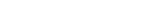
\includegraphics{ch07/figs/inductor-symbol}},
has no resistance; the resistor $R$ has no inductance. It is
this idealized circuit that we shall now analyze.

If the current $I$ in the circuit is changing at the rate $\der I/\der t$, an electromotive
force $L\: \der I/\der t$ will be induced, in a direction to oppose the
change. Also, there is the constant electromotive force $\emf_0$ of the
% p. 253
battery. If we define the positive current direction as the one in
which the battery tends to drive current around the circuit, then the
net electromotive force at any instant is $\emf_0 - L\: \der I/\der t$. This drives
the current $I$ through the resistor $R$. That is,
\begin{equation}
  \emf_0 - L\frac{\der I}{\der t} = RI
\end{equation}

We can also describe the situation in this way: The potential difference
between points $A$ and $B$, which we'll call the \emph{voltage across
the inductor}, is $L\: \der I/\der t$, with the upper end of the inductor positive
if $I$ in the direction shown is \emph{increasing}. The potential difference
between $B$ and $C$, the voltage across the resistor, is $RI$, with the upper
end of the resistor positive. Hence the sum of the voltage across the
inductor and the voltage across the resistor is $L\: \der I/\der t+RI$. This is
the same as the potential difference between the battery terminals,
which is $\emf_0$ (our idealized battery has no internal resistance). Thus
we have
\begin{equation}
  \emf_0 = L\frac{\der I}{\der t} + RI
\end{equation}
which is merely a restatement of Eq. 60.

Before we look at the mathematical solution of Eq. 60, 1et's predict
what ought to happen in this circuit if the switch is closed at $t = 0$.
Before the switch is closed, $I = 0$, necessarily. A long time after the
switch has been closed, some steady state will have been attained,
with current practically constant at some value $I_0$. Then and there-
after, $\der I/\der t\approx 0$, and Eq. 60 reduces to
\begin{equation}
  \emf_0 = RI_0
\end{equation}
The transition from zero current to the steady-state current $I_0$ cannot
occur abruptly at $t = 0$, for then $\der I/\der t$ would be infinite. In fact,
just after $t = 0$, the current $I$ will be so small that the second term
$RI$ in Eq. 60 can be ignored, giving
\begin{equation}
  \frac{\der I}{\der t} = \frac{\emf_0}{L}
\end{equation}
The inductance $L$ limits the rate of rise of the current.

What we now know is summarized in Fig. 7.24a. It only remains
to find how the whole change takes place. Equation 60 is a differential 
equation like some you have already met in Sec. 4.11 and in
% p. 254
Vol. 1, Chap. 6. Without further ado we can write down a solution
to Eq. 60 which satisfies our initial condition, $I = 0$ at $t = 0$.
\begin{equation}
  I = \frac{\emf_0}{R}\left(1-e^{-(R/L)t}\right)
\end{equation}

The graph in Fig. 7.24b shows the current approaching its asymptotic
value $I_0$ exponentially. The ``time constant'' of this circuit is
the quantity $L/R$. If $L$ is measured in henrys and $R$ in ohms, this
comes out in seconds, since $\zu{henrys} \sim \zu{vo1ts}/ (\zu{A}/\sunit)$, and
$\zu{ohms} \sim \zu{volts}/\zu{A}$.

What happens if we open the switch after the current $I_0$ has been
established, thus forcing the current to drop abruptly to zero? That
would make the term $L\: \der I/\der t$ negatively infinite! The catastrophe
can be more than mathematical. People have been killed opening
switches in highly inductive circuits. What happens generally is that
a very high induced voltage causes a spark or are across the open
switch contacts, so that the current continues after all. Let us instead
remove the battery from the circuit by closing a conducting
path \emph{across} the $LR$ combination, as in Fig. 7.25a, at the same time 
disconnecting the battery. We now have a circuit described by the
equation
\begin{equation}
  0 = L \frac{\der I}{\der t} +RI
\end{equation}
with the initial condition $I = I_0$ at $t = t_1$, where $t_1$ is the instant at
which the short circuit was closed. The solution is the simple exponential
decay function:
\begin{equation}
  I = I_0 e^{-(R/L)(t-t_1)}
\end{equation}
with the same characteristic time, $L/R$, as before.

\iffalse

\section{Energy stored in the magnetic field}
During the decay of the current described by Eq. 66 and Fig. 7.2511,
energy is dissipated in the resistor R. Since the energy d U dissipated

in any short interval dt is R12 dt, the total energy dissipated after
the closing of the switch at time t1 must be:

\begin{equation}
\end{equation}
U = °°R12 dt = °°RI02e~<2R/L><t-m dt (67)

% p. 255
With the substitution x = 2B(t - t1)/L this is easily evaluated:

\begin{equation}
\end{equation}
U = R102 f0°°e-I dx = iuoz (68)

The source of this energy was the inductor with its magnetic field.
Indeed, exactly that amount of work had been done by the battery
to build up the current in the first place---over and above the energy
dissipated in the resistor between t = 0 and t = t1, which was also
provided by the battery. To see that this is a general relation, note
that if we have an increasing current in an inductor, work must be
done to drive the current I against the induced electromotive force
L (II/dt. So in time dt the work done is

ff

\begin{equation}
\end{equation}
dW: LI dt

dt = LI dI =iLd(12) (69)

Therefore, we may assign a total energy
\begin{equation}
\end{equation}
U = §LI2 (70)

to an inductor carrying current I. With the eventual decay of this
current, that amount of energy will appear somewhere else.

It is natural to regard this as energy stored in the magnetic field
of the inductor, just as we have described the energy of a charged
capacitor as stored in its electric field. The energy of a capacitor
charged to potential difference V is §CV2, and is accounted for by
assigning to an element of volume do, where the electric field strength
is E, an amount of energy (1/87r)E2 do. It is pleasant, but hardly
surprising, to find that an exactly similar relation holds for the energy
stored in an inductor. That is, we can ascribe to the magnetic field
an energy density (1/87r)B2, and summing the energy of the whole
field will give the energy §LI2.

To show how this works out in one case, we can go back to the
toroidal coil whose inductance L we calculated in Sec. 7.8. We
found (Eq. 58)

\begin{equation}
\end{equation}
L = 2W' In (E) (71)

02 a
The magnetic field strength B, with current I flowing, was given

\begin{equation}
\end{equation}
B : 2NI
cr

(72)

% p. 256
To calculate the volume integral of B2/8w we can use a volume element
consisting of the cylindrical shell sketched in Fig. 7.26, with
volume Zvrrh dr. As this shell expands from r = a to r = b, it sweeps
through all the space that contains magnetic field. (The field $\vc{B}$ is
zero everywhere outside the torus, remember.)

\begin{equation}
\end{equation}
1 1 b2NI 2 N2h12 I9
WfB2dv:87  Cr ) 27rrhdr: $C_2$ ln(;) (73)

Comparing this result with Eq. 71, we see that, indeed,

\begin{equation}
\end{equation}
1
8---WfB2 do = %LI2 (74)

The more general statement, the counterpart of our statement for
the electric field in Eq. 1.36, is that the energy U to be associated with
any magnetic field B(x,y,z) is given by:

\begin{equation}
\end{equation}
(75)

 

With B in gauss and v in cubic centimeters, U in Eq. 75 will be given
in ergs. In Eq. 70, we may use practical units, henrys and amperes,
for L and I, and then U will be given in joules.

\section{``Something is missing''}

Let us review the relations between charges and fields. As we
learned in Chap. 2, a statement equivalent to Coulomb's law is the
differential relation

\begin{equation}
\end{equation}
div E = 4'n'p (76)

connecting the electric charge density p and the electric field E. This
holds for moving charges as well as stationary charges. That is, p can
be a function of time as well as position. As we emphasized in
Chap. 5, the fact that Eq. 76 holds for moving charges is consistent
with charge invariance: No matter how an isolated charged particle
may be moving, its charge, as measured by the integral of $\vc{E}$ over a
surface surrounding it, appears the same in every frame of reference.

% p. 257
Electric charge in motion is electric current. Because charge is
never created or destroyed, the charge density p and the current
density J always satisfy the condition

\begin{equation}
\end{equation}
divJ= _@ (77)

We first wrote down this ``Equation of Continuity'' as Eq. 4.9.
If the current density J is constant in time, we call it a stationary

current distribution. The magnetic field of a stationary current distribution
satisfies the equation

\begin{equation}
\end{equation}
curl B = 4T'"J (78)

We worked with this relation in Chap. 6.

Now we are interested in charge distributions and fields that are
changing in time. Suppose we have a charge distribution p(x,y,z,t)
with Bp/at sé 0. For instance, we might have a capacitor which is

discharging through a resistor. According to Eq. 77, ap/at7&O
implies

\begin{equation}
\end{equation}
div J yé O (79)

But according to Eq. 78, since the divergence of the curl of any
vector function is identically zero (see Prob. 2.15),

\begin{equation}
\end{equation}
div J = L div (curl B) = 0 (80)
477'

The contradiction shows that Eq. 78 cannot be correct for a system
in which the charge density is varying in time. Of course, no one
claimed it was; a stationary current distribution, for which Eq. (78)
does hold, is one in which not even the current density J, let alone the

charge density p, is time-dependent.
The problem can be posed in somewhat different terms by considering
the line integral of magnetic field around the wire carrying

charge away from the capacitor plate in Fig. 7.27. According to
Stokes' theorem,

\begin{equation}
\end{equation}
fen-d1=Lcur1B-da (81)

The surface $S$ passes right through the conductor in which a current
I is flowing. Inside this conductor, $\curl\vc{B}$ has a finite value,
namely 47rJ/0, and the integral on the right comes out equal to 4771/c.
That is to say, if the curve C is close to the wire and well away from
the capacitor gap, the magnetic field there is not different from the

% p. 258
field around any wire carrying the same current. Now the surface S'
in Fig. 7.28 is also a surface spanning C, and has an equally good
claim to be used in the statement of Stokes' theorem, Eq. 81.
Through this surface, however, there flows no current at all! Never-
theless, $\curl\vc{B}$ cannot be zero over all of S' without violating Stokes'
theorem. Therefore, on S', $\curl\vc{B}$ must depend on something other
than the current density J.

We can only conclude that Eq. 78 has to be replaced by some

other relation, in the more general situation of changing charge dis-
tributions. Let's write instead

\begin{equation}
\end{equation}
curl B = 47% + ('2) (82)

and see if we can discover what ('?) must be.

Another line of thought suggests the answer. Remember that the
transformation laws of the electromagnetic field, Eq. 6.58, are quite
symmetrical in $\vc{E}$ and B. Now in Faraday's induction phenomenon
a changing magnetic field is accompanied by an electric field, in a
manner described by our Eq. 30:

\begin{equation}
\end{equation}
curl E = _ ii (30)

cat

% p. 259
This is a local relation connecting the electric and magnetic fields in
empty space-charges are not directly involved. If symmetry with
respect to $\vc{E}$ and $\vc{B}$ is to prevail, we must expect that a changing electric
field can give rise to a magnetic field. There ought to be an induction
phenomenon described by an equation like Eq. 30, but with
the roles of $\vc{E}$ and $\vc{B}$ switched. It will turn out that we need to change
the sign too, but that is all:

curl B = :7} (83)

This provides the missing term that is called for in Eq. 82. To
try it out, write

\begin{equation}
\end{equation}
cui1B=4T"J+%-%% (84)
and take the divergence of both sides:

\begin{equation}
\end{equation}
div (curl B) = div (EJ) + div (LE) (85)
c c at

The left side is necessarily zero, as already remarked. In the second
term on the right we can interchange the order of differentiation with
respect to space coordinates and time. Thus

\begin{equation}
\end{equation}
.1aE_ia. _477Bp
'""(:7) - cw""VE) 'T73? (86)

by Eq. 76. The right-hand side of Eq. 85 now becomes

\begin{equation}
\end{equation}
- div J + --- (87)

which is zero by virtue of the continuity condition, Eq. 77.

The new term resolves the difficulty raised in Fig. 7.28. As charge
flows out of the capacitor, the electric field, which at any instant has
the configuration in Fig. 7.29, diminishes in intensity. In this case,

\begin{equation}
\end{equation}
1 BE

BE/at points opposite to E. The vector function $F$ E is represented
by the black arrows in Fig. 7.30. With curl B = 4T7TJ + %-aa%, the

integral of $\curl\vc{B}$ over S' now has the same value as it does over S.
On 8' the second term contributes everything; on $S$ the first term, the
term with J, is practically all that counts.

% p. 260
% p. 261
\section{The displacement current}

Observe that the vector field L 381;; appears to form a continuation

c

of the conduction current distribution. Maxwell called it the displacement
current, and the name has stuck although it no longer
seems very appropriate. To be precise, we can define a ``displace-
ment current density" J,,,, to be distinguished from the conduction
current density J, by writing Eq. 84 this way:

\begin{equation}
\end{equation}
curl B = 4_:(J + Jd) (88)
and defining J,,, E 

We needed the new term to make the relation between current and
magnetic field consistent with the continuity equation, in the case
of conduction currents changing in time. If it belongs there, it
implies the existence of a new induction effect in which a changing
electric field is accompanied by a magnetic field. If the eff'ect is real,
why didn't Faraday discover it? For one thing, he wasn't looking
for it, but there is a more fundamental reason why experiments like
F araday's could not have revealed any new effects attributable to the
last term in Eq. 84. In any apparatus in which there are changing
electric fields, there are present at the same time conduction currents,
charges in motion. The magnetic field B, everywhere around the
apparatus, is just about what you would expect those conduction
currents to produce. In fact, it is almost exactly the field you would
calculate if, ignoring the fact that the circuits may not be continuous,
you used the ``Biot-Savart'' formula, Eq. 6.38, to find the contribution
of each conduction current element to the field at some point in space.

Consider, for example, the point P in the space between our discharging
condenser plates, Fig. 7.31. Each element of conduction
current, in the wires and on the surface of the plates, contributes to
the field at P, according to the Biot-Savart formula. Must We include
also the elements of ``displacement current'' Jd? The answer is rather
surprising. We may include Jd; but if we are careful to include the
entire displacement current distribution, its net effect will be zero for
relatively slowly varying fields.

To see why this is so, notice that the vector function J,,;, indicated
by the black arrows in Fig. 7.30, has the same form as the electric
field $\vc{E}$ in Fig. 7.29. This electric field is practically an electrostatic
field, except that it is slowly dying away. We expect therefore that
its curl is practically zero which would imply that curl J must be

% p. 262
practically zero. More precisely, we have curl E = - L311 and

cat

with the displacement current Jd = Li, we get, by interchang-

47r at
ing the order of differentiation,

\begin{equation}
\end{equation}
curl J,,, = 4L7Tcur1  = 4-£T-5a;(curl E) = -  (89)
This will be negligible for sulficiently slow changes in field. We
may call a slowly changing field quasi-static. Now if Jd is a vector
field without any curl, it can be made up, in the same way that the
electrostatic field can be made of the fields of point charges, by superposing
radial currents flowing outward from point sources or in
toward point ``sinks'' (Fig. 7.32). But the magnetic field of any
radial, symmetrical current distribution, calculated (1 la Biot-Savart,

must be zero by symmetry, for there is no unique direction anywhere,
except the radial direction itself.

In the quasi-static field, then, the conduction currents alone are
the only sources needed to account for the magnetic field. In other
words, if Faraday had arranged something like Fig. 7.31, and had
been able to measure the magnetic field at P, by using a compass
needle say, he would not have been surprised. He would not have
needed to invent a displacement current to explain it.

% p. 263
To see this new induction effect, we need rapidly changing fields.
In fact, we need changes to occur in the time it takes light to cross
the apparatus. That is why the direct demonstration had to wait for

Hertz, whose experiment came many years after the law itself had
been worked out by Maxwell.

\section{Maxwell's equations}

James Clerk Maxwell, after immersing himself in the accounts of
Faraday's electrical researches, set out to formulate mathematically
a theory of electricity and magnetism. Maxwell could not exploit
re1ativity---that came fifty years later. The electrical constitution
of matter was a mystery, the relation between light and electromagnetism
unsuspected. Many of the arguments that we have used to
make our next step seem obvious were unthinkable then. Neverthe-
less, as Maxwell's theory developed, the term we have been discuss-
ing, 6E/at, appeared quite naturally in his formulation. He called
it the ``displacement current.'' Maxwell was concerned with electric
fields in solid matter as well as in vacuum, and when he talks about
a ``displacement current'' he is often including some charge-in-
motion, too. We'll clarify that point in Chap. 9 when we study electric
fields in matter. Indeed, Maxwell thought of space itself as a
medium, the ``aether,'' so that even in the absence of solid matter the
displacement current was occurring in something. But never mind---
his mathematical equations were perfectly clear and unambiguous,
and his introduction of the displacement current was a theoretical
discovery of the first rank. 

Maxwell's description of the electromagnetic field was essentially
complete. We have arrived by different routes at various pieces of it,
which we shall now assemble in the form traditionally called
Maxwell 's equations:

\begin{equation}
\end{equation}
(90)

 

These are written for the fields in vacuum, in the presence of electric

charge of density p and electric current, that is, charge-in-motion,
of density J.

in

% p. 264
The first equation is Faraday's law of induction. The second
expresses the dependence of the magnetic field on the displacement
current density, or rate-of-change of electric field, and on the conduction
current density, or rate-of-motion of charge. The third
equation is equivalent to Coulomb's law. The fourth equation states
that there are no sources of magnetic field except currents. We shall
have more to say about this aspect of Nature in Chap. 10.

Notice that the lack of symmetry in these equations, with respect
to $\vc{B}$ and E, is entirely due to the presence of electric charge and elec-

tric conduction current. In empty space, the terms with p and J are
zero, and Maxwell's equations become

\begin{equation}
\end{equation}
(91)

 

Here the displacement current term is all-important. Its presence,
along with its counterpart in the first equation, implies the possibility
of electromagnetic waves. Recognizing that, Maxwell went on to
develop with brilliant success an electromagnetic theory of light.
You will be exploring the physics of waves, and of light waves in
particular, in Vol. III. We can show right now that an electromagnetic
disturbance traveling at speed c is compatible with Maxwell's
equations. To do this, we shall describe a very simple set of electric
and magnetic fields which represent a traveling disturbance, and
then we shall show that these fields satisfy all the equations in the
box, Eqs. 91.

At the instant of time t = 0, there exists, we suppose, an electric
field in the region between the planes y = 0 and y = 2a. This field E

has a z component only, and its z component depends only on y, in
the following manner:

\begin{equation}
\end{equation}
Ez=E0% <o:y:a>
(at time t = 0) (92)

2 - _ _
Ee=EO( "Q 9) (a2y22a>
As indicated in Fig. 7.33a, this describes a ``gable''-shaped distribution
of field strength, maximum in the center at y = a and falling off
linearly to zero at y = a and g = 2a. For given y, the field is the
same at all x and z. That is, we have electric field throughout an

% p. 265
% p. 266
infinite slab, although in the figure we show field vectors on the y axis
only. The shaded patches marked I and II lie within this slab.
Everywhere outside the slab, that is, for y < O and y > 2a, the electric
field is zero at this instant of time. At the same time a magnetic
field $\vc{B}$ exists in this slab of space. It has an x component only.
given by:

\begin{equation}
\end{equation}
Bz=B0% (05y§a)
(at time t = O) (93)

B,=Bo(2"a"') <a:y:2a>

We simply invented this field. Let us now command the field
configuration to travel in the y direction with speed 0, while preserving
its shape. We can do that by writing out orders as follows:

\begin{equation}
\end{equation}
Region 1:
E2 = E0 (y - ct)
Cl _ _
_ Ct (ct 2 y 2 at + a) (94)
B' : B0 (y a )


\begin{equation}
\end{equation}
Region II:
2 _
E, : E0  _ _
20- +Ct (ct+a2y2ct+2a) (95)
Bx = Bo <+)

This describes the situation as we see it in Fig. 7.3312, or at any other
time t. The region containing field is simply displaced to the right
by a distance at. Within regions I and II, both $\vc{E}$ and $\vc{B}$ have the same
form as before. Our equations, then, describe a traveling configuration
of electric and magnetic fields, but can such fields exist? To
answer that, we must see if $\vc{E}$ and B, as given by Eqs. 94 and 95, satisfy
Maxwell's equations.

Beginning with the divergence equations, it is easy to see that
div E = 0 and $\div\vc{B}$ = 0. (Obviously 6E,/Bz = O and the other
components of $\vc{E}$ are themselves zero.) But $\curl\vc{E}$ is not zero.
Instead, its value is:

In Region I: V x E _-_ ii = f;

\begin{equation}
\end{equation}
(96)
In Region II: V x E = $2 = -

% p. 267
In the same way we calculate V x B:

In Regionlz VxB= -i aaB' = -%i
9
\begin{equation}
\end{equation}
(97)
In Region 11; VxB= -2 33" =l3£2
By a
The partial derivatives with respect to t are:
In Region 1: 1;. = _ EEO2 fig. = _ £302
a a
\begin{equation}
\end{equation}
(98)
In Region II: % : %E0i % : %Box

The fields will satisfy the "induction" equations in region I, then, if

E , 1 ,
7°' = ':('§B°")
and B I C (99)
__°2 =_(_ -1202)
a C a

Indeed, these are satisfied provided E0 = B0. The equations lead
to exactly the same requirement for the fields in region II. Exactly
at the peak of the gable, and also at each end, there are mathematical
singularities in the assumed fields. To be sure that the field equations
are satisfied everywhere, we must see that there is no trouble at these
points. There is none, because $\vc{E}$ and $\vc{B}$ are continuous there. (An
abrupt jump. or discontinuity, in $\vc{E}$ or $\vc{B}$ would not be possible in
empty space.) Thus the particular electromagnetic field we have
described. which does represent a traveling wave, does satisfy all the
field equations, if the electric field, in statvolts/cm, is everywhere
equal to the magnetic field strength, at the same time and place. It is
essential that $\vc{E}$ and $\vc{B}$ be perpendicular to one another and to the
direction of travel---otherwise the field equation could not have been
satisfied.

Our traveling ``gable'' may strike you as a rather special kind of
wave. In fact, this simple example reveals all that is essential about
any plane electromagnetic wave! We need only think of super-
position. As we have frequently emphasized, the equations of the
electromagnetic field are linear. If two sets of fields satisfy Maxwell's
equations, so does their sum. We can have any number of our
``gable'' fields traveling through space, in the same or different direc-
tions. (Naturally, the fields don't care how the axes are oriented-

% p. 268
any other direction is as good as the y axis.) Fig. 7.34 suggests some
of the waves you could make with ``gables.'' It is pretty obvious that
any function could be approximated as closely as desired by superposing
``gables.'' Therefore, what we have learned about the gable
wave must apply to any wave in which $\vc{E}$ and $\vc{B}$ are functions only
of the coordinate in the direction of travel. These general facts are:

(i) The disturbance travels with speed c, with unchanging
form. 

(ii) $\vc{E}$ and $\vc{B}$ are perpendicular to each other and to the direction
of travel, with the vector E x B always pointing in the
direction of the travel, as it does in our example.

(iii) At a given point and time, E = B.

An electromagnetic field with these properties transforms in a
simple and satisfying way when we change coordinate systems. In
Chap. 6 we derived formulas for the Lorentz transformation of the
electric and magnetic fields (Eq. 6.58). Let's use the results of
Prob. 6.11, which were based on those equations, according to which
the two scalar quantities, E2 - B2 and E - B remain invariant in a
transformation to another inertial frame. In this case, since E = B
at any point, the invariant quantity E2 - B2 has the value zero. Also.
because $\vc{E}$ is perpendicular to B, the other invariant E - B is zero. It
follows that in any other frame the transformed fields $\vc{E}'$ and $\vc{B}'$ must
be equal to each other in magnitude and perpendicular in direction.
A light wave looks like a light wave in any frame of reference.

\fi

\chapter{Alternating-current circuits}

\section{A resonant circuit}

A circuit containing inductance, capacitance, and resistance was
one of the examples of the damped harmonic oscillator discussed in
Vol. 1, Chap. 7. Now we can see exactly what goes on in that system.
The circuit diagram in Fig. 8.1 represents such a ``series $RLC$'' circuit.

Let $Q$ be the charge, at time $t$, on the capacitor in this circuit. The
potential difference, or voltage across the capacitor, is $V$, which
obviously is the same as the voltage across the series combination
of inductor $L$ and resistor $R$. We take $V$ to be positive when the upper
capacitor plate is positively charged, and we define the positive current
direction by the arrow in Fig. 8.1. With the signs chosen that
way, the relations connecting charge $Q$, current $I$, and voltage across
the capacitor $V$ are:
\begin{equation}
  I=-\frac{\der Q}{\der t} \qquad
  Q = CV \qquad
  V=L\frac{\der I}{\der t}+RI
\end{equation}
We want to eliminate two of the three variables $Q$, $I$, and $V$. From
the first two equations we obtain $I = - C \der V/\der t$, and the third equation
becomes $V = -LC(\der^2V/\der t^2) - RC(\der V/\der t)$, or
\begin{equation}
  \frac{\der^2V}{\der t^2} + \left(\frac{R}{L}\right) \frac{\der V}{\der t} + \left(\frac{1}{LC}\right) V = 0
\end{equation}

This is a second-order differential equation with constant 
coefficients. We shall try a solution of the form
\begin{equation}
  V = A e^{-\alpha t}\cos\omega t
\end{equation}
where $A$, $\alpha$, and $\omega$ are constants. The first and second derivatives of
this function are:
\begin{align}
  \frac{\der V}{\der t} &=    A e^{-\alpha t}[-\alpha\cos\omega t-\omega\sin\omega t] \\
  \frac{\der^2V}{\der t^2} &= A e^{-\alpha t}[(\alpha^2-\omega^2)\cos\omega t+2\alpha\omega\sin\omega t]
\end{align}
% p. 275
Substituting back into Eq. 2, we cancel out the common factor $A e^{-\alpha t}$
and are left with
\begin{equation}
  (\alpha^2-\omega^2)\cos\omega t+2\alpha\omega\sin\omega t
       -\frac{R}{L}(\alpha\cos\omega t+\omega\sin\omega t)
       +\frac{1}{LC}\cos\omega t = 0
\end{equation}
This will be satisfied for all $t$ if, and only if, the coefficients of $\sin \omega t$
and $\cos\omega t$ are both zero. That is, we require:
\begin{equation}
  2\alpha\omega-\frac{R\omega}{L} = 0
\end{equation}
and
\begin{equation}
  \alpha^2-\omega^2-\alpha\frac{R}{L}+\frac{1}{LC} = 0
\end{equation}
The first of these equations gives a condition on $\alpha$:
\begin{equation}
  \alpha = \frac{R}{2L}
\end{equation}
while the second equation requires that:
\begin{equation}
  \omega^2 = \frac{1}{LC}-\alpha \frac{R}{L} + \alpha^2 = \frac{1}{LC}-\frac{R^2}{4L^2}
\end{equation}

Since our constant $\omega$ is a real number, $\omega^2$ cannot be negative.
Therefore we succeed in obtaining a solution of the form assumed in
Eq. 3 only if $R^2/4L^2\le 1/LC$. In fact it is the case of ``light
damping,'' that is, low resistance, that we want to examine, so we
shall assume that the values of $R$, $L$, and $C$ in the circuit are such that
the inequality $R < 2\sqrt{L/C}$ holds.

The function $A e^{-\alpha t}\cos\omega t$ is not the only possible solution.
$B e^{-\alpha t}\sin\omega t$ works just as well, with the same requirements, Eq. 9 and
Eq. 10, on $\alpha$ and $\omega$. The general solution is the sum of
these:
\begin{equation}
  V(t) = e^{-\alpha t}(A\cos\omega t+B\sin\omega t)
\end{equation}
V(t) = e'"'(A cos wt + B sin wt) (11)

The arbitrary constants $A$ and $B$ could be adjusted to fit initial
conditions. That is not very interesting. Whether the solution in
any given case involves the sine or the cosine function, or some 
superposition, is a trivial matter of how the clock is set. The essential
phenomenon is a damped sinusoidal oscillation.

% p. 276

The variation of voltage with time is shown in Fig. 8.2a. Of course,
this cannot really hold for all \emph{past} time. At some time in the past
the circuit must have been provided with energy somehow, and then
left running. For instance, the capacitor might have been charged,
with the circuit open, and then connected to the coil.

In Fig. 8.2b the time scale has been expanded and the dotted curve
showing the variation of the current $I$ has been added. For $V$ let us
take the damped cosine, Eq. 3. Then the current as a function of time
is given by:
\begin{equation}
  I = -C\frac{\der V}{\der t} = AC\omega\left(\sin\omega t+\frac{\alpha}{\omega}\cos\omega t\right)e^{-\alpha t}
\end{equation}
The ratio $\alpha/\omega$ is a measure of the damping. If $\alpha/\omega$ is very small,
many oscillations occur while the amplitude is decaying only a little.
For Fig. 8.2 we chose a case in which $\alpha/\omega\approx 0.04$. Then the cosine
term in Eq. 12 doesn't amount to much. All it does, in effect, is shift
the phase by a small angle, $\tan^{-1}(\alpha/\omega)$. So the current oscillation
is almost exactly one-quarter cycle out of phase with the voltage
oscillation.

The oscillation involves a transfer of energy back and forth from
the capacitor to the inductor, or from electric field to magnetic field.
At the times marked 1 in Fig. 8.2b all the energy is in the electric field.
A quarter-cycle later, at 2, the capacitor is discharged and nearly all
this energy is found in the magnetic field of the coil. Meanwhile, the
circuit resistance R is taking its toll, and as the oscillation goes on,
the energy remaining in the fields gradually diminishes.

The relative damping in an oscillator is often expressed by giving a
number called $Q$.\index{quality factor|see{Q}}\index{Q of an oscillator}
This was introduced in the general discussion of
harmonic oscillators in Vol. 1, Chap. 7. $Q$ (not to be confused with
the charge on the capacitor!) is said to stand for ``quality'' or ``quality
factor.'' In fact, no one calls it that; we just call it ``$Q$.'' The less
the damping, the larger the number $Q$. For an oscillator with frequency
$\omega$, $Q$ is the dimensionless ratio formed as follows:
\begin{equation}
  Q = \omega\frac{\text{energy stored}}{\text{average power dissipated}}
\end{equation}
Or you may prefer to remember that $Q$ is the number of radians of
the argument $\omega t$ (that is, $2\pi$ times the number of cycles) required for
the energy in the oscillator to diminish by the factor $1/e$.

% p. 278

In our circuit the stored energy is proportional to $V^2$ or $I^2$ and,
therefore, to $e^{-2\alpha t}$. The energy decays by $1/e$ in a time $t = 1/2\alpha$,
which covers $\omega/2\alpha$ radians. Hence for our $RLC$ circuit
\begin{equation}
  Q = \frac{\omega}{2\alpha} = \frac{\omega L}{R}
\end{equation}
As a rough estimate, what is the $Q$ of the oscillation represented in
Fig. 8.2?

Clearly, the general case we have just studied includes some simple
special cases. If $R = 0$ we have the completely undamped oscillator,
whose frequency $\omega_0$ is given by
\begin{equation}
  \omega_0 = \frac{1}{\sqrt{LC}}
\end{equation}
Mostly we deal with systems in which the damping is small enough
to be ignored in calculating the frequency. As Prob. 8.9 will 
demonstrate, damping has only a second-order effect on $\omega$.

For completeness we review brieffy what goes on in the 
overdamped circuit, in which $R > 2\sqrt{L/C}$. Equation 2 then has a solution
of the form $V = Ae^{-\beta t}$ for two values of $\beta$, the general solution
being
\begin{equation}
  V(t) = Ae^{-\beta_1 t}+Be^{-\beta_2 t}
\end{equation}
There are no oscillations, only a monotonic decay. In the special
case of ``critical'' damping, $R = 2\sqrt{L/C}$, $\beta_1=\beta_2$ and the solution
of the differential equation, Eq. 2, takes the form
\begin{equation}
  V(t) = (A + Bt)e^{-\beta t}
\end{equation}
This is the condition, for given L and C, in which the total energy
in the circuit is most rapidly dissipated. (See Prob. 8.8.)

You can see this whole range of behavior in Fig. 8.3, where $V(t)$ is
plotted for two underdamped circuits, a critically damped circuit,
and an overdamped circuit. The capacitor and inductor remain the
same; only the resistor is changed. The natural angular frequency
$\omega_0 = 1/\sqrt{LC}$ is $10^6\ \sunit^{-1}$ for this circuit, corresponding to a frequency
in cycles per second of $10^6/2\pi$, or 159 kHz.

The circuit is started off by charging the capacitor to a potential
difference of, say, 1 volt and then closing the switch at $t = 0$. That
is, $V = 1$ at $t = 0$ is one initial condition. Also, $I = 0$ at $t = 0$, because
the inductor will not allow the current to rise discontinuously.
Therefore, the other initial condition on $V$ is $\der V/\der t = 0$, at $t = 0$.
% p. 279
Notice that all four decay curves start the same way. In the heavily
damped case ($R = 600\ \text{ohms}$) most of the decay curve looks like
the simple exponential decay of an $RC$ circuit. Only the very beginning
where the curve is rounded over so that it starts with zero slope,
betrays the presence of the inductance $L$.

\iffalse

\section{Alternating current}

The resonant circuit we have just discussed contained no source
of energy and was, therefore, doomed to a transient activity, an
oscillation that must sooner or later die out. In an alternating-
current circuit we are concerned with a steady state, a current and
voltage oscillating sinusoidally without change in amplitude. Some
oscillating electromotive force drives the system.

Let us apply an electromotive force 8 = 80 cos wt to a circuit containing
inductance and resistance. We might generate 8 by a
machine schematically like the one in Fig. 7.13, having provided
some engine or motor to turn the shaft at the constant angular
speed ea. In Fig. 8.4 this electromotive force is represented as connected
into the circuit. We shall neglect any internal resistance in
the generator, or include it in R. We set the sum of potential drops
over the element of this circuit equal to the electromotive force 8,

exactly as we did in developing Eq. 7.61. The equation governing
the current is then:

\begin{equation}
\end{equation}
Lff

dt + R1 = 80 cos wt (18)

Now there may be some transient behavior, depending on the
initial conditions, that is, on how and when the generator is switched
on. But we are interested only in the steady state, when the current
is oscillating obediently at the frequency of the driving force, with
the amplitude and phase necessary to keep Eq. 18 satisfied. To show
that this is possible, consider a current described by

\begin{equation}
\end{equation}
I = 10 cos (wt + (p) (19)

To determine the constants I0 and $\pot$, we put this into Eq. 18:
\begin{equation}
\end{equation}
-LI0w sin (wt + q:) - RIO cos (wt + go) = 80 cos wt (20)
The functions cos wt and sin wt can be separated out:

-LI0w(sin wt cos (p + cos wt sin (p)
+RI0(cos wt cos (p - sin wt sin (p) = 80 cos wt (21)

 

% p. 280
 
 

Setting the coefficients of cos wt and sin wt separately equal to zero,

\begin{equation}
\end{equation}
-LI0w cos (p - RIO sin cp = 0 (22)
which gives
tan go 2 - EH14 (23)
-LI0w sin (p + R10 cosgb _ 50 = 0 (24)
which gives
1 _ }:530____
0- RCOS(p- coLSin<;0
_ 80 _ 80 cos (1) 2
- R(cos<p+ sinqotan qJ) _ R ( 5)
or since
cos - _L- (from E 23) (26)
'P " \/1W,7,2'L7 q'
10 = 8° (27)

, /R2 + w2L2

In Fig. 8.5 the oscillations of 8 and I are plotted on the same graph.
Since $\pot$ is a negative angle, the current reaches its maximum a bit
later than the electromotive force. One says, ``The current lags the
voltage in an inductive circuit.'' The quantity wL which has the
dimensions of resistance and can be expressed in ohms is called the
inductive reactance.

If we replace the inductor L by a capacitor C, as in Fig. 8.6, we
have a circuit governed by the equation

\begin{equation}
\end{equation}
- % + HI = 80 cos wt (28)

We consider the steady-state solution
\begin{equation}
\end{equation}
I = 10 cos (wt + (p) (29)
Since I _-_ -dQ/dt, we have
\begin{equation}
\end{equation}
Q=_f1dt=_I_°sin(wt+<p) (30)
00
Note that in going from I to Q by integration, there is no question

of adding a constant of integration, for we know that Q must oscillate
symmetrically about zero in the steady state.

% p. 281
Substituting back into Eq. 28 leads to

\begin{equation}
\end{equation}
1_0

C sin (wt + (p) + RIO cos (cot + (p) = 80 cos wt (31)
(.0

Just as before, we obtain conditions on go and 10 by requiring that the
coelficients of cos wt and sin wt separately vanish. In this case, the
results are:

\begin{equation}
\end{equation}
l
RwC

tan q) : 

and

10 = :8'; (33)

\/R2 + (l/wC)2

Notice that the phase angle is now positive. As the saying goes, the
current ``leads the Voltage'' in a capacitive circuit. What this means
is apparent in the graph of Fig. 8.7.

Mathematically speaking, the function

\begin{equation}
\end{equation}
_ 80 _ OJL
I _ \/---1  cos (wt - tan 1 Y) (34)

is a particular integral of the differential equation, Eq. 18. To this
could be added a complementary function, that is, any solution of
the homogeneous differential equation

\begin{equation}
\end{equation}
dI _
L? + RI _ 0 (35)

Now this is just Eq. 765, whose solution we found, in Sec. 7.9, to be
an exponentially decaying function,

\begin{equation}
\end{equation}
1 ~ e-<R/L» (36)

The physical significance is this: A transient, determined by some

 

  

initial conditions, is represented by a decaying component of I (t), _

of the form of Eq. 36. After a time t > L/R, this will have vanished
leaving only the steady sinusoidal oscillation at the driving frequency,
represented by the particular integral, Eq. 34.

The similarity of our results for the RL circuit and the RC circuit
suggests a way to look at the inductor and capacitor in series.
Suppose an alternating current I = I0 cos (wt + q)) is somehow

% p. 282
 
 

caused to flow through such a combination (shown in Fig. 8.8). The
voltage across the inductor, VL, will be:

\begin{equation}
\end{equation}
VL = L:ii-£ = -IowL sin (wt + (p) (37)

The Voltage Vg across the capacitor, with sign consistent with the sign
Of VL, lS

\begin{equation}
\end{equation}
1 I .
V0 : - % = -C-JTdt = +)Cs1n (wt + 90) (38)

The voltage across the combination is then

\begin{equation}
\end{equation}
v=vL+vc= _ (wL_%)10sin(wt+(p) (39)
For a given an, the combination is evidently equivalent to a single ele-
ment, either an inductor or a capacitor, depending on whether the

1 .
quantity (ooL - TC) is positive or negative. Suppose, for example,

that wL >  Then the combination is equivalent to an inductor
OJ

L' such that

\begin{equation}
\end{equation}
, 1

wL _ wL - E (40)
Equivalence means only that the relation between current and
voltage, for steady oscillation at the particular frequency w, is the
same. This allows us to replace L and C by L' in any circuit driven

at this frequency.
This can be applied to the simple RLC circuit in Fig. 8.9. We need
only recall Eqs. 23 and 27, the solution for the RL circuit driven by

the electromotive force 80 cos wt, and replace wL by wL - l/coC:

\begin{equation}
\end{equation}
_ 50
tan (p = RLW _ '~1'TL (42)

For fixed amplitude 80 of the electromotive force, and given circuit
elements L, C, and R, we get the greatest current when the driving
frequency co is such that

\begin{equation}
\end{equation}
1

-:= 4
wL wc 0 (3)

% p. 283
which is the same as saying that w = 1/ LC = «:0, the resonant
frequency of the undamped LC circuit. In that case Eq. 39 reduces to

\begin{equation}
\end{equation}
80 COS wt

I: R

(44)

This is exactly the current that would flow if the circuit contained
the resistor alone.

As an example, consider the circuit of Fig. 8.3a, connected now
to a source or generator of alternating emf, 8 = 80 cos cat. The driving
frequency to may be different from the resonant frequency
we = 1/ \/IT', which, for the given capacitance (0.01 microfarads)
and the inductance (100 microhenrys), is 106 radians/ sec (or 106/2w
cycles/sec). Figure 8.10 shows the amplitude of the oscillating cur-
rent, as a function of the driving frequency w, for three different

R = 20 ohms

% p. 284
values of the circuit resistance R. It is assumed that the amplitude 80
of the emf is 100 volts in each case. Notice the resonance peak at
w = we, which is most prominent and sharp for the lowest resistance
value. This is the same value of R for which, running as a damped
oscillator without any driving emf, the circuit behaved as shown in
the top graph of Fig. 8.31).
The Qofthe circuit definedb E 14 L ' -___('°6 X 10%)
, y q. as «>0 /R,'l' IS 20 .
or 5, in this case. Generally speaking, the higher the Q of a circuit,
the narrower and higher the peak of its response as a function of
driving frequency co. To be more precise, consider frequencies in
the neighborhood of mo, writing a: = mg + Aw. Then to first order
in Aw/coo, the expression wL - 1/o.>C which occurs in the denomi-

nator in Eq. 41 can be approximated this way:

\begin{equation}
\end{equation}
1 < Aw) I
L _ - = L 1 - _ L; 45
"' "'° 'L w0C(l + Aw/mo) ( )

woL [1 + A1 - -L-] : woL (2 fo-:°) (46)

Exactly at resonance, the quantity inside the square root sign in
Eq. 41 is just R2. As on is shifted away from resonance the quantity
under the square root will have doubled when |wL - l/wC| = R,
or when, approximately,

\begin{equation}
\end{equation}
2Aw R l
= = - 47
000 LOOL Q ( )

This means that the current amplitude will have fallen to 1/ \/7 times
the peak when Aw/coo = 1/2Q. These are the ``half-power'' points.
because the energy, or power is proportional to the amplitude
squared, as we shall explain in Sec. 8.5. One often expresses the
width of a resonance peak by giving the full width between half-
power points. Evidently that is just 1/ Q times the resonant frequency
itself. Circuits with very much higher Q than this one are
quite common. A radio receiver may select a particular station and

TThe w in Eq. 14 was the frequency of the freely decaying damped oscillator, practically
the same as too for moderate or light damping. We use we here in the definition
of Q. In the present discussion to is any frequency we may choose to apply to this circuit.

% p. 285
discriminate against others by the help of a resonant circuit with a Q
of several hundred. It is quite easy to make a microwave resonant
circuit with a Q of 104, or even 105.

The angle q), which expresses the relative phase of the current and
emf oscillations, varies with frequency in the manner shown in
Fig. 8.11. At a very low frequency the capacitor is the dominant
hindrance to current flow, and (p is positive. At resonance, (p = 0.
The higher the Q, the more abruptly $\pot$ shifts from positive to negative
angles as the frequency is raised through coo.

\section{Alternating-current networks}

An alternating-current network is any collection of resistors,
capacitors, and inductors in which currents flow that are oscillating
steadily at the constant frequency to. One or more electromotive
forces, at this frequency, drive the oscillation. Figure 8.12 is a diagram
of one such network. . The source of alternating electromotive
force is represented by the symbol  In a branch of the network,

for instance the branch that includes the inductor L2, the current as
a function of time is

\begin{equation}
\end{equation}
I2 = 102 COS (wt + (pg) 

Since the frequency is a constant for the whole network, two num-
bers, such as the amplitude I02 and the phase constant (122 above, are
enough to determine for all time the current in a particular branch.

 

% p. 286
Similarly, the voltage across a branch oscillates with a certain
amplitude and phase:

\begin{equation}
\end{equation}
V2 : V02 COS (wt + 02) 

If we have determined the currents and voltages in all branches of
a network, we have analyzed it completely. To find them by constructing
and solving all the appropriate differential equations is
possible, of course; and if we were concerned with the transient behavior
of the network, we might have to do something like that. For
the steady state, however, we can use a far simpler and more elegant
method. It is based on two ideas:

(i) An alternating current or voltage can be represented by a
complex number.

(ii) Any one branch or element of the circuit can be charac-
terized, at a given frequency, by the relation between the
voltage and current in that branch.

The first idea exploits that remarkable mathematical identity
\begin{equation}
\end{equation}
e" = cos 0 + 2' sin 0 (50)

with i2 = - 1. To carry it out we adopt the following rule for the
representation:

  

An alternating current 10 cos (wt + q:) is to be represented
by the complex number Ioeiw, that is, the number whose real
part is I0 cos q: and whose imaginary part is 10 sin tp.

Going the other way, if the complex number x + iy represents
a current I, then the current as a function of time is given
by the real part of the product (3: + iy)ei~'.

      
   
 
    

Figure 8.13 is a reminder of this two-way correspondence. Since
a complex number z = x + iy can be graphically represented on the
two-dimensional plane, it is easy to visualize the phase constant as
the angle tan'1 y/x, and the amplitude Io as the modulus 

What makes all this useful is the following fact: The representation
of the sum of two currents is the sum of their representations. Consider
the sum of two currents I1 and 12 that meet at a junction of wires in
Fig. 8.12. At any instant of time t the sum of the currents is:

\begin{equation}
\end{equation}
11 + 12 = 101 C08 (cot + (pi) + 102 cos (wt + (P2)

= (101 cos (p1 + 102 cos (P2) cos wt
- (I01 Sl1'l (P1 + 102 SlI'l (P2) SlI'l wt 

% p. 287
On the other hand, the sum of the complex numbers that, according
to our rule, represent I1 and I2 is:

\begin{equation}
\end{equation}
1016*?' + 10291" = (101 005 'P1 + 102 005 #32)
+ i(Io1 Sin 'P1 + 102 Sin (P2) (52)

If you multiply the right-hand side of Eq. 52 by (cos wt + i sin wt)
and take the real part of the result, you will get just what appears or
the right in Eq. 51.

This means that instead of adding or subtracting the periodic functions
of time themselves, we can add or subtract the complex numbers
that represent them. Or putting it another way, the algebra of alternating
currents turns out to be the same as the algebra of complex
numbers, in respect to addition. The correspondence does not extend
to multiplication. The complex number Io1I02e"W1+W2) does not
represent the product of the two current functions in Eq. 51.

However, it is only the addition of currents and voltages that we
need to carry out in analyzing the network. For example, at the
junction where 11 meets 12 in Fig. 8.12, there is the physical requirement
that at every instant the net flow of current into the junction
shall be zero. Hence the condition

\begin{equation}
\end{equation}
I1-{-I2-I-13:0 

must hold, where 11, I2, and 13 are the actual periodic functions of
time. Thanks to our correspondence, this can be expressed in the

% p. 288
simple algebraic statement that the sum of three complex numbers
is zero. Voltages can be handled in the same way. Instantaneously,
the sum of the voltage drops around any loop in the network must
equal the electromotive force in the loop at that instant. This condition
relating periodic voltage functions can likewise be replaced by
a statement about the sum of some complex numbers, the representations
of the various oscillating functions, V1(t), V2(t), etc.

\section{Admittance and impedance}

The relation between current flow in a circuit element and the
voltage across the element can be expressed as a relation between the
complex numbers that represent the voltage and the current. Look
at the inductor-resistor combination in Fig. 8.4. The voltage oscillation
is represented by 80 and the current by Ioetw, where 10 =
80/ x/B2 + ML? and tan go = -wL/R. The phase difference (p and
the ratio of current amplitude to voltage amplitude are properties

of the circuit at this frequency. We define a complex number Y as
follows:

\begin{equation}
\end{equation}
eiw
, /R2 +?w2L2

Then the relation

\begin{equation}
\end{equation}
wL

Y = with (,5 = tan'1<- -R-) (54)

\begin{equation}
\end{equation}
1 = YV (55)

holds, where V is the complex number that represents the Voltage
across the series combination of R and L, and I is the complex number
that represents the current. Y is called the admittance. The

same relation can be expressed with the reciprocal of Y, denoted by
Z and called the impedance:

\begin{equation}
\end{equation}
V =  I = Z1 (56)

Here we do make use of the product of two complex numbers, but
only one of the numbers is the representation of an alternating current
or Voltage. The other is the impedance or admittance.T

TOur algebra thus contains two categories of complex numbers, those that represent
impedances, for example, and those that represent currents. The product of two

``impedance numbers,'' like the product of two ``current numbers,'' doesn't represent
anything.

% p. 289
The impedance is measured in ohms. Indeed, if the circuit element
had consisted of the resistance R alone, the impedance would
be real and equal simply to R, so that Eq. 56 would resemble Ohm's
law for a direct-current circuit: V = R1.

The admittance of a resistanceless inductor is the imaginary
quantity Y = -i/wL. This can be seen by letting R go to zero in
Eq. 54. The factor ---i shows that the current oscillation lags the
voltage oscillation by 77/2 in phase. On the complex number dia-
gram, if the voltage is represented by V (Fig. 8.1419), the current
might be represented by I, located as shown there. For the capacitor,
Y = icoC, as can be seen from the expression for the current in
Fig. 8.7. In this case V and I are related as indicated in Fig. 8.140.
The inset in each of the figures shows how the relative sign of Vand I
is to be specified. Unless that is done consistently, ``leading'' and
``lagging'' are meaningless. Note that we always define the positive
current direction so that a positive voltage applied to a resistor causes
positive current (Fig. 8.l4a).

The properties of the three basic circuit elements are summarized
below:

Symbol Admittance, Y Impedance, Z = LY
R L R
JWW R
L  1'¢..>L
'\U.Qr wL
C .
' C ;'
_H- W wC
I = YV V = Z1

We can build up any circuit from these elements. When elements
or combinations of elements are connected in parallel, it is convenient
to use the admittance, for in that case admittances add. In Fig. 8.15
two ``black boxes'' with admittances Y1 and Y2 are connected in
parallel. We have then

\begin{equation}
\end{equation}
I = 11 + 12 = Y1V+ Y2V= (Y1 + Y2)V (57)

% p. 290
  

which implies that the equivalent single black box has an admittance
Y = Y1 + Y2. From Fig. 8.16 it will be obvious that the impedances
add for elements connected in series. It sounds as if we are talking
about a direct-current network! In fact, we have now reduced the
ac network problem to the dc network problem, with only this dif-
ference: the numbers we deal with arecomplex numbers.

As an example, let's look at the ``parallel RLC'' circuit in
Fig. 8.17. The combined admittance of the three parallel branches is

\begin{equation}
\end{equation}
_L - _;'
Y_R+1wC COL (53)

The voltage is simply 80, so the complex current is
\begin{equation}
\end{equation}
1: YV= s0[-+i(wc_i)] (59)

The amplitude of the current oscillation is the modulus of the complex
number I, which is 80[(l/R)? + (wC - 1/wL)2]1/2, and the
phase angle is tan'1 (RwC - R/wL).

We can only deal in this way with linear circuit elements, elements
in which the current is proportional to the voltage. In other words,
our circuit must be described by a linear differential equation. You
can't even define an impedance for a nonlinear element. Nonlinear
circuit elements are very important and interesting devices. You
have studied some in the laboratory, and you can see why they will
not readily yield to this kind of analysis.

This is all predicated, too, on the continuous oscillation at constant
frequency. The transient behavior of the circuit is a different
problem. However, for linear circuits the tools we have just developed
have some utility, even for transients. The reason is that by
superposing steady oscillations of many frequencies we can represent
a nonsteady behavior, and the response to each of the individual
frequencies can be calculated as if that frequency were present alone.
This can well be left for Volume III.

\section{Power and energy in alternating-current circuits}
If the voltage across a resistor R is V0 cos cat, the current is
I : (V0/R) cos Lot. The instantaneous power, that is the instantaneous
rate at which energy is being dissipated in the resistor is
V02

\begin{equation}
\end{equation}
P = R12 = T cos? wt (60)

% p. 291
Since the average of cos? out over many cycles is %, the average power
dissipated in the circuit is

\begin{equation}
\end{equation}
1 V02

P=_:
2 R

(61)

It is customary to express voltage and current in ac circuits by giving
not the amplitude but 1/ \/7 times the amplitude. This is often called
the ``root-mean-square'' or, for short, ``rms'' value. That takes care
of the factor 4 in Eq. 61, so that

\begin{equation}
\end{equation}
V%ms
R

P:

(62)

For example, the common domestic line voltage, 120 volts, corresponds
to an amplitude 120\/7 volts. The potential difference be-

tween the terminals of the electric outlet in your room (if the voltage
is up to normal) is

\begin{equation}
\end{equation}
V(t) = 170 cos 377t (63)

with Vin volts and t in seconds. An ac ammeter is calibrated to read
1 amp when the current amplitude is 1.414 amperes.

In general, the instantaneous rate at which energy is delivered to
a circuit element is VI, the product of the instantaneous voltage and
current, with due regard to sign. Consider this aspect of the current
flow in the simple LR circuit in Fig. 8.4. In Fig. 8.18 we have redrawn
the current and voltage graphs and added a curve proportional to
the product VI. Positive VI means energy is being transferred into
the LR combination from the source of electromotive force, or
generator. Notice that VI is negative in certain parts of the cycle.
In those periods some energy is being returned to the generator.
This is explained by the oscillation in the energy stored in the magnetic
field of the inductor. This stored energy, §LI2, goes through
a maximum twice in each full cycle.

The average power, 13, corresponds to the horizontal dashed line.
To calculate its value, let's look at the product V1, with V = 80 cos out
and 1 : 10 cos (wt + (P):

\begin{equation}
\end{equation}
VI = 8010 cos cot cos (cot + (p)
: 80I0(cos 2 cot cos (p - cos cot sin wt sin (p) (64)

% p. 292
oped in Sec. 8.4, we'll analyze
an, 1-watt resistor has been
pacitance 0.2 and 0.5 micro-
5 into the 120-volt, 60-cycle
>r get too hot? In the course
:r dissipated in R exceeds the
he currents and voltages we
One way to work through the

7) (2 x 10'7)i
'41' ohm'1

: 10_4 OhII1_1
+ 0.754i) ohm'1

1
+ 0.7541')

. 0.754:-)
0.7542

- 4800:') ohms

1
(377) (5 X 10'7)
LS
360 - 10,1001') ohms

0 + 10,1001')
+ (10,100)?

1e rms voltage, we obtain the
re complex number 11, which
or 10.0 milliamperes (mA),
illiammeter inserted in series
; current has a phase angle
ns with respect to the line
to the entire circuit is then:

; 1.01 = 0.64 watt

% p. 293
R and L in series

B and C in series

R, L, and C in parallel

In this circuit the resistor is
be the average power dissip
the voltage V2 across the re:

\begin{equation}
\end{equation}
(ix) V1 = 11: (5.3

= (45.2 _ 28.41') ~
(x) V2 = 120 - V1 = (7A

The current 12 in R will be ll
power in R will be

\begin{equation}
\end{equation}
P=L2 =_(

R

which checks.

Thus the rating of the r
surance is worth. Actually
pends not only on the avera
easily it can get rid of the he
a rough guide.

\fi

\chapter{Electric fields in matter}

\section{Dielectrics}

The capacitor we studied in Chap. 3 consisted of two conductors,
insulated from one another, with nothing in between. The system
of two conductors was characterized by a certain capacitance $C$, a
constant relating the magnitude of the charge Q on the capacitor
(positive charge $Q$ on one plate, equal negative charge on the other)
to $V_{12}$, the difference in electrical potential between the two 
conductors:
\begin{equation}
  C = \frac{Q}{V_{12}}
\end{equation}
For the parallel-plate capacitor, two flat plates each of area $A\ \cmunit^2$
and separated by a distance $t$, we found that the capacitance is
given by
\begin{equation}
  C = \frac{A}{4\pi t}
\end{equation}
Capacitors like this can be found in some electrical apparatus. They
are called \emph{vacuum capacitors}\index{capacitor!vacuum}
and consist of plates enclosed in a highly
evacuated bottle. They are used chiefly where extremely high and
rapidly varying potentials are involved. Far more common, how-
ever, are capacitors in which the space between the plates is filled
with some nonconducting solid or liquid substance. Most of the
capacitors you have worked with in the laboratory are of that sort;
there are dozens of them in any television receiver. For conductors
embedded in a material medium, Eq. 2 doesn't agree with experiment.
Suppose we fill the space between the two plates shown in Fig. 9.1a
with a slab of plastic, as in Fig. 9.1b. Experimenting with this new
capacitor, we still find a simple proportionality between charge and
potential difierence, so that we can still \emph{define} a capacitance by Eq. 1.
But we find $C$ to be substantially \emph{larger} than Eq. 2 would 
predict.

Not only in the special devices called capacitors, but almost everywhere
in the world around us, the electric and magnetic fields exist
in the presence of matter rather than in a vacuum --- if not in dense
matter, then at least in a gas, namely air. All this is to remind us
that, except for our excursion in Chap. 4 into the subject of electrical
conduction, we have really been studying the electromagnetic field
in empty space populated only by certain point charges or smooth
% p. 299
charge distributions. Now we must seek to understand the interactions
of electric and magnetic fields with matter in bulk.

Two different approaches are open to us. Maintaining a large-scale,
or \emph{macroscopic}, point of view, we could see how the presence
of a block of homogeneous material like the plastic slab in Fig. 9.lb
affects the electric field in the space outside, where we can measure
the field. We could try to discover simple laws which would adequately
describe such effects in any system of conductors and in-
sulators. We would find that the macroscopic electric behavior of
homogeneous substances can indeed be characterized fairly simply
and completely. Equation 2, for example, needs only the insertion
on the right-hand side of a constant factor 5, characteristic of the particular
substance, to give correctly the capacitance of any capacitor
filled with that material. $\epsilon$ is called the \intro{dielectric constant} of that
substance, and the material itselfis generally referred to as a dielectric
when we are considering its behavior in an electric field. Dielectric
constants of some common substances are listed in Table \ref{table:dielectric-constants}. Once
the dielectric constant of a particular material has been determined,
perhaps by measuring the capacitance of one capacitor filled with it,
% p. 300
we are able to predict the behavior, not merely of two-plate 
capacitors, but of any electrostatic system made up of conductors and
pieces of that dielectric of any shape. That is, we can predict all
electric fields which will exist in the vacuum outside the dielectrics
for given charges or potentials on the conductors in the system.

\begin{table} % makes it floating
\caption{Dielectric constants of various substances}\label{table:dielectric-constants}
\begin{tabular}{lll}
\hline
\emph{Substance} & \emph{Conditions} & \emph{Dielectric constant} \\
\hline
Air                             & Gas, 0\degcunit, 1 atm & 1.00059 \\
Hydrogen chloride, HCl          & Gas, 0\degcunit, 1 atm & 1.0046 \\
Water, $\zu{H}_2\zu{O}$                      & Gas, 110\degcunit, 1 atm & 1.0126 \\
                                & Liquid, 20\degcunit & 80 \\
Benzene, $\zu{C}_6\zu{H}_6$               & Liquid, 20\degcunit        & 2.28 \\
Ammonia, $\zu{NH}_3$               & Liquid,  $-34\degcunit$    & 22 \\
Transformer oil               & Liquid, 20\degcunit      & 2.24 \\
Sodium chloride, NaCl           & Crystal, 20\degcunit               & 6.12 \\
Sulfur, S                 & Solid, 20\degcunit           & 4.0 \\
Quartz, $\zu{SiO}_2$                    & Crystal, 20\degcunit\ ($\perp$ optic axis)       & 4.34 \\
                                & Crystal, 20\degcunit\ ($\parallel$ optic axis)   & 4.27 \\
Polyethylene                 & Solid, 20\degcunit        & 2.25-2.3 \\
Neoprene                 & Solid, 20\degcunit            & 4.1 \\
Porcelain                 & Solid, 20\degcunit           & 6.0-8.0 \\
Paraffin wax                 & Solid, 20\degcunit        & 2.1-2.5 \\
Pyrex glass 7070                 & Solid, 20\degcunit    & 4.00
\end{tabular}
\end{table}

The theory which enables us to do this was fully worked out by
the physicists of the nineteenth century. Lacking a complete picture
of the atomic structure of matter, they were more or less obliged to
adopt a macroscopic description. From that point of view, the interior
of a dielectric is a featureless expanse of perfectly smooth
``mathematical jelly'' whose single electrical property distinguishing
it from a vacuum is a dielectric constant different from unity.

If we develop only a macroscopic description of matter in an
electric field, we shall find it hard to answer some rather obvious-
sounding questions --- or rather, hard to ask these questions in such
a way that they can be meaningfully answered. For instance, what
is the strength of the electric field \emph{inside} the plastic slab of Fig. 9.lb
when there are certain charges on the plates? Electric field strength
is defined by the force on a test charge. How can we put a test charge
inside a perfectly dense solid, without disturbing anything, and
measure the force on it? What would that force mean, if we did
measure it? You might think of boring a hole and putting the test
charge in the hole with some room to move around, so that you can
measure the force on it as on a free particle. But then you will be
measuring, not the electric field in the dielectric, but the electric field
in a cavity in the dielectric, which is quite a different thing.

Fortunately another line of attack is available to us, one that leads
up from the microscopic or \emph{atomic} level. We know that matter is
made of atoms and molecules; these in turn are composed of elementary
charged particles. We know something about the size and
structure of these atoms, and we know something about their arrangement
in crystals and fluids and gases. Instead of describing our
dielectric slab as a volume of structureless but nonvacuous jelly, we
shall describe it as a collection of molecules inhabiting a vacuum.
If we can find out what the electric charges in \emph{one} molecule do when
that molecule is all by itself in an electric field, we should be able to
understand the behavior of two such molecules a certain distance
apart in a vacuum. It will only be necessary to include the influence,
on each molecule, of any electric field arising from the other. This
is a vacuum problem. Now all we have to do is extend this to a population
of say $10^{20}$ molecules occupying a cubic centimeter or so of
% p. 301
vacuum, and we have our real dielectric. We hope to do this without
generating $10^{20}$ separate problems.

This program if carried through will reward us in two ways. We
shall be able at last to say something meaningful about the electric
and magnetic fields inside matter, answering questions such as the
one raised above. What is more valuable, we shall understand how
the macroscopic electric and magnetic phenomena in matter arise
from, and therefore reveal, the nature of the underlying atomic 
structure. We are going to study electric and magnetic effects separately.
We begin with dielectrics. Since our first goal is to describe the electric
field produced by an atom or molecule, it will help to make some
general observations about the electrostatic field external to any small
system of charges.

\section{The moments of a charge distribution}

An atom or molecule consists of some electric charges occupying
a small volume, perhaps \linebreak[4]$\sim (0.1\ \zu{nm})^3=10^{-24}\ \cmunit^3$ of space.
We are interested in the electric field outside that volume, which
arises from this rather complicated charge distribution. We shall
be particularly concerned with the field far away from the source,
by which we mean far away compared to the size of the source itself.
What features of the charge structure mainly determine the field at
remote points? To answer this, let's look at some arbitrary distribution
of charges and see how we might go about computing the field
at a point outside it. Figure 9.2 shows a charge distribution of some
sort located in the neighborhood of the origin of coordinates. It
might be a molecule consisting of several positive nuclei and quite
a large number of electrons. In any case we shall suppose it is described
by a given charge density function $\rho(x,y,z)$. $\rho$ is negative
where the electrons are and positive where the nuclei are. To find
the electric field at distant points we can begin by computing the
potential of the charge distribution. To illustrate, let's take some
point $A$ out on the $z$ axis. (Since we are not assuming any special
symmetry in the charge distribution, there is nothing special about
the $z$ axis.) Let $r$ be the distance of $A$ from the origin. The electric
potential at $A$, denoted by $\pot_A$, is obtained as usual by adding the
contributions from all elements of the charge distribution:
\begin{equation}
  \pot_A = \int \frac{\rho(x',y',z')\:\der v'}{R}
\end{equation}
% p. 302
In the integrand $\der v'$ is an element of volume within the charge 
distribution, $\rho(x',y',z')$ is the charge density there, and $R$ in the denominator
is the distance from $A$ to this particular charge element. The
integration is carried out in the coordinates $x'$, $y'$, $z'$, of course, and
is extended over all the region containing charge. We can express $R$
in terms of $r$ and the distance $r'$ from the origin to the charge element.
Using the law of cosines with $\theta$ the angle between $r'$ and the axis on
which $A$ lies:
\begin{equation}
  R = [r^2 + r'^2 - 2rr'\cos\theta]^{1/2}
\end{equation}
With this substitution for $R$ the integral becomes:
\begin{equation}
  \pot_A = \int \rho\:\der v'[r^2 + r'^2 - 2rr'\cos\theta]^{-1/2}
\end{equation}
Now we want to take advantage of the fact that for a distant point
like $A$, $r'$ is much smaller than $r$ for all parts of the charge distribution.
This suggests that we should expand the square root in Eq. 4 in
powers of $r'/r$. Writing
\begin{equation}
  [r^2 + r'^2 - 2rr'\cos\theta]^{-1/2} 
      = \frac{1}{r}\left[1+\left(\frac{r'^2}{r^2}-\frac{2r'}{r}\cos\theta\right)\right]^{-1/2}
\end{equation}
and using the expansion $(1+\delta)^{-1/2}=1-\frac{1}{2}\delta+\frac{3}{8}\delta^2\ldots$, we get,
after collecting together terms of the same power in $r'/r$:
\begin{equation}
  [r^2 + r'^2 - 2rr'\cos\theta]^{-1/2}
   = \frac{1}{r}\left[1+\frac{r'}{r}\cos\theta
                       +\left(\frac{r'}{r}\right)^2\frac{(3\cos^2\theta-1)}{2}
                       +\left(\begin{array}{cc}\text{terms of}\\\text{higher power}\end{array}\right)\right]
\end{equation}
Now $r$ is a constant in the integration, so we can take it outside and
write the prescription for the potential at $A$ as follows:
\begin{equation}
  \pot_A =
        \frac{1}{r}  \underbrace{\int\rho\:\der v'}_{K_0}
       +\frac{1}{r^2}\underbrace{\int r'\cos\theta\:\rho\:\der v'}_{K_1}
       +\frac{1}{r^3}\underbrace{\int r'^2\frac{(3\cos^2\theta-1)}{2}\rho\:\der v'}_{K_2}
       +\ldots
\end{equation}
Each of the integrals above, $K_0$, $K_1$, $K_2$, and so on, has a value that
depends only on the structure of the charge distribution. Hence the
% p. 303
potential for all points along the $z$ axis can be written as a power series
in $1/r$ with constant coefficients:
\begin{equation}
  \pot_A = \frac{K_0}{r}+\frac{K_1}{r^2}+\frac{K_2}{r^3}+\ldots
\end{equation}

To finish the problem we would have to get the electric field at all
other points, in order to calculate the electric field as  $-\operatorname{grad}\pot$. We
have gone far enough, though, to bring out the essential point: The
behavior of the potential at large distances from the source will be
dominated by the first term in this series whose coefficient is not zero.

Let us look at these coefficients more closely. The coeflicient $K_0$
is $\int\rho\:\der v'$, which is nothing but the total charge in the distribution.
If we have equal amounts of positive and negative charge, as in a
neutral molecule, $K_0$ will be zero. For a singly ionized molecule $K_0$
will have the value $e$. If $K_0$ is not zero, then no matter how large
$K_1$, $K_2$, etc., may be, if we go out to a sufliciently large distance the
term $K_0/ r$ will win out. Beyond that, the potential will approach that
of a point charge at the origin and so will the field. This is hardly
surprising.

Suppose we have a neutral molecule, so that $K_0$ is zero. Our interest
now shifts to the second term, with coefficient $K_1 = \int r'\cos\theta\:\rho\:\der v'$.
Since $r' \cos \theta$ is simply $z'$, this term measures the relative 
displacement, in the direction toward $A$, of the positive and negative charge.
It has a nonzero value for the distributions sketched in Fig. 9.3, where
the densities of positive and of negative charge have been indicated
separately. In fact, all the distributions shown there have approximately
the same value of $K_1$.

It is worth noting that if the distribution is neutral the value of $K_1$
is independent of the position of the origin. That is, if we replace
$z'$ by $(z' + z_0')$, thus in effect shifting the origin, the value of the integral
is not changed: $\int(z' + z_0')\rho\:\der v' = \int z'\rho\: \der v' + z_0'\int\rho\:\der v'$ and the
latter integral is always zero for a neutral distribution.

Evidently if $K_0 = 0$ and $K_1\ne 0$, the potential along the $z$ axis will
vary asymptotically (that is, with ever-closer approximation as we
go out to larger distances) as $1/r^2$. We expect the electric field
strength, then, to behave asymptotically like $1/r^3$, in contrast to the
$1 /r^2$ dependence of the field from a point charge. Of course we have
discussed only the potential on the $z$ axis. We will return to the question
of the exact form of the field after getting a general view of the
situation.

% p. 304

If $K_0$ and $K_1$ are both zero, and $K_2$ is not, the potential will behave
like $1/r^3$ at large distances, and the field strength will fall off with
the inverse fourth power of the distance. Figure 9.4 shows a charge
distribution for which $K_0$ and $K_1$ are both zero (and would be zero
no matter what direction we had chosen for the $z$ axis) while $K_2$ is
not zero.

The quantities $K_0$, $K_1$, $K_2$, \ldots are related to what are called the
\emph{moments}\index{moments} of the charge distribution. Using this language, we call $K_0$,
which is simply the net charge, the \intro{monopole moment}, or \emph{monopole
strength}. $K_1$ is one component of the \intro{dipole moment} of the 
distribution. The dipole moment has the dimensions \emph{charge} times 
\emph{displacement}; it is a vector and our $K_1$ is its $z$ component. The third
constant $K_2$ is related to the \intro{quadrupole moment} of the distribution,
the next to the \intro{octupole moment}, and
so on.\footnote{It can be shown that decomposition of the source into various \intro{multipoles}, if carried
through completely, uniquely specifies the charge distribution. In other words, if we
know all the multipole strengths we can ``in principle'' deduce $\rho(x',y',z')$. This is not
very useful. The quadrupole and higher moments are not vectors, by the way, but
more complicated entities.}

The advantage to us of describing a charge distribution by this
hierarchy of moments is that it singles out just those features of the
charge distribution which determine the field at a great distance. If
we were concerned only with the field in the immediate neighborhood
of the distribution, it would be a fruitless exercise. For our main task,
understanding what goes on in a dielectric, it turns out that \emph{only} the
monopole strength (the net charge) and the dipole strength of the
molecular building blocks matter. We can ignore all other moments.
And if the building blocks are neutral, we have only their dipole
moments to consider.

\section{The potential and field of a dipole}

The dipole contribution to the potential at the point $A$, distance
$r$ from the origin, was given by $(1/r^2)\int r' \cos \theta\:\rho\:\der v'$. We can write
$r' \cos \theta$, which is just the projection of $\vc{r}'$ on the direction toward $A$,
as $\hat{\vc{r}}\cdot\vc{r}'$. Thus we can write the potential without reference to any
arbitrary axis as
\begin{equation}
  \pot_A = \frac{1}{r^2}\int \hat{\vc{r}}\cdot\vc{r}'\rho\:\der v'
      = \frac{\rhat}{r^2}\cdot\int \vc{r}'\rho\:\der v'
\end{equation}
which will serve to give the potential at any point. The integral on
the right in Eq. 9 is the \emph{dipole moment} of the charge distribution. It
% p. 305
is a vector, obviously, with the dimensions \emph{charge} times \emph{distance}. We
shall denote the dipole moment vector by $\vc{p}$:
\begin{equation}
  \vc{p} = \int \vc{r}'\rho\:\der v'
\end{equation}
Using the dipole moment $\vc{p}$, we can rewrite Eq. 9 as
\begin{equation}
  \pot(\vc{r}) = \frac{\rhat\cdot\vc{p}}{r^2}
\end{equation}
The electric field is the negative gradient of this potential. To see
what the dipole field is like, locate a dipole $\vc{p}$ at the origin, pointing
in the $z$ direction (Fig. 9.5). With this arrangement,
\begin{equation}
  \pot = \frac{p\cos\theta}{r^2}
\end{equation}
% p. 306
The potential and the field are, of course, symmetrical around the
$z$ axis. Let's work in the $xz$ plane, where $\cos \theta = z/ (x^2 + z^2)^{1/2}$. In
that plane,
\begin{equation}
  \pot = \frac{pz}{(x^2 + z^2)^{3/2}}
\end{equation}
The components of the electric field are:
\begin{align}
\begin{split}
  E_x = -\frac{\partial\pot}{\partial x} &= \frac{3pxz}{(x^2 + z^2)^{5/2}} = \frac{3p\sin\theta\cos\theta}{r^3} \\
  E_z = -\frac{\partial\pot}{\partial z} 
   &= p\left[\frac{3z^2}{(x^2 + z^2)^{5/2}}-\frac{1}{(x^2 + z^2)^{3/2}}\right] \\
   &= \frac{p(3\cos^2\theta-1)}{r^3}
\end{split}
\end{align}

Proceeding out in any direction from the dipole, we find the electric
field strength falling off as $1/r^3$, as we had anticipated. Along
the $z$ axis the field is parallel to the dipole moment $\vc{p}$, with magnitude
$2p/r^3$. In the equatorial plane the field points antiparallel to $\vc{p}$ and
has the value $-\vc{p}/r^3$.

This field may remind you of one we have met before. Remember
the point charge over the conducting plane, with its ``image charge.''
% p. 307
The simplest charge distribution with a dipole moment is two
point charges, $+q$ and  $-q$, separated by a distance $s$. For a system
of point charges Eq. 10 takes the form of a sum. The dipole moment
of our point-charge pair is just $qs$, and the vector points in the direction
from negative charge to positive. In Fig. 9.6 we have sketched
the field of this pair of charges, mainly to emphasize that the field
near the charges is \emph{not} a dipole field. This charge distribution has
many multipole moments, indeed infinitely many, so it is only the
``far field'' at distances $r \gg s$ that can be represented as a dipole field.

To generate a complete dipole field right in to the origin we would
have to let $s$ shrink to zero while increasing $q$ without limit so as to
keep $p = qs$ finite. This highly singular abstraction is not very 
interesting. We know that our molecular charge distribution will have
complicated near fields, so we could not easily represent the near
region in any case. Fortunately we shall not need to.

\section{The torque and the force on a dipole in an external field}

Suppose two charges $q$ and  $-	q$ are mechanically connected so
that $s$, the distance between them, is fixed. You may think of the
charges as stuck on the end of a short nonconducting rod of length $s$.
We shall call this object a dipole. Its dipole moment $p$ is simply $qs$.
Let us put the dipole in an external electric field, that is, the field from
some other source. The field of the dipole itself does not concern
us now. Consider first a uniform electric field, as in Fig. 9.7a. The
positive end of the dipole is pulled toward the right, the negative end
toward the left, by a force of strength $Eq$. The net force on the object
is zero and so is the torque, in this position. A dipole which makes
some angle $\theta$ with the field direction as in Fig. 9.7b obviously experiences
a torque. In general, torque $\btorque$ is $\vc{r} \times \vc{F}$ where $\vc{F}$ is the force
applied at a distance $\vc{r}$ from the origin (Vol. 1, Chap. 6). Taking the
origin in the center of the dipole, so that $r = s/2$, we have
\begin{equation}
  \btorque = \vc{r}\times\vc{F}_+ + (-\vc{r})\times\vc{F}_-
\end{equation}
$\btorque$ is a vector perpendicular to the figure, and its magnitude is:
\begin{equation}
  \tau = \frac{s}{2}Eq\sin\theta + \frac{s}{2}Eq\sin\theta = sqE\sin\theta = pE\sin\theta
\end{equation}
This can be written simply
\begin{equation}
  \btorque = \vc{p}\times\vc{E}
\end{equation}

% p. 308

The orientation of the dipole in Fig. 9.7a has the lowest energy.
Work has to be done to rotate it into any other position. Let us calculate
the work required to rotate the dipole from a position parallel
to the field, through some angle $\theta_0$, as shown in Fig. 9.7c. Rotation
through an infinitesimal angle $\der\theta$ requires an amount of work $\torque\:\der\theta$
Thus the total work done is
\begin{equation}
  \int_0^{\theta_0} \torque\:\der\theta 
    = \int_0^{\theta_0} pE\sin\theta\:\der\theta
    = pE(1-\cos\theta_0)
\end{equation}
To reverse the dipole, turning it end for end, corresponds to $\theta_0=\pi$
and requires an amount of work equal to $2pE$.

The net force on the dipole in any \emph{uniform} field is zero, obviously.
regardless of its orientation. In a nonuniform field the forces on the
two ends of the dipole will generally not be exactly equal and 
opposite, and there will be a net force on the object. A simple example
is a dipole in the field of a point charge $Q$. If the dipole is oriented
radially as in Fig. 9.8a, with the positive end nearer the positive
charge $Q$, the net force will be outward, and its magnitude will be
\begin{equation}
  F = (q)\frac{Q}{r^2}+(-q)\frac{Q}{(r+2)^2}
\end{equation}
For $s\ll r$, we need only evaluate this to first order in $s/r$, which we
do as follows:
\begin{equation}
  F = \frac{qQ}{r^2}\left[1-\frac{1}{\left(1+\frac{s}{r}\right)^2}\right]
    \approx \frac{qQ}{r^2}\left[1-\frac{1}{1+\frac{2s}{r}}\right]
    \approx \frac{2sqQ}{r^3}
\end{equation}
In terms of the dipole moment $p$, this is simply
\begin{equation}
  F = \frac{2pQ}{r^3}
\end{equation}

With the dipole at right angles to the field, as in Fig. 9.8b, there is
also a force. Now the forces on the two ends, though equal, are not
exactly opposite in direction.

It is not hard to work out a general formula for the force on a dipole
in a nonuniform electric field. The force depends essentially on the
gradients of the various components of the field. In general, the
$x$ component of the force on a dipole of moment $\vc{p}$ is
\begin{equation}
  F_x = \vc{p}\cdot\operatorname{grad} E_x
\end{equation}
with corresponding formulas for $F_y$ and $F_z$.

% p. 309

\section{Atomic and molecular dipoles; induced dipole moments}

In describing the charge distribution in an atom or molecule we
shall have to use classical terms to depict a quantum mechanical
system. Also, we shall be treating as static a structure in which the
particles are, in some sense, continually in motion. Later in the
course, in Vol. IV, you will see how quantum mechanics, far from discrediting
the picture we are about to sketch, reassuringly supports it.

Consider the simplest atom, the hydrogen atom, which consists of
a nucleus and one electron. If you imagine the negatively charged
electron revolving around the positive nucleus like a planet around
the sun --- as in the original atomic model of Niels Bohr\index{Bohr model} --- you will
conclude that the atom has, at any one instant of time, an electric
dipole moment. The dipole moment vector $\vc{p}$ points parallel to the
electron-proton radius vector, and its magnitude is $e$ times the
electron-proton distance. The direction of this vector is continually
and rapidly changing as the electron circles around its orbit. To be
sure, the \emph{time average} of $\vc{p}$ will be zero for a circular orbit, but we
should expect the periodically changing dipole moment components
to generate rapidly oscillating electric fields and electromagnetic
radiation. The absence of such radiation in the normal hydrogen
atom was one of the great paradoxes of early quantum physics.
Modern quantum mechanics tells us that it is better to think of the
hydrogen atom in its lowest energy state (the usual condition of most
of the hydrogen atoms in the universe) as a spherically symmetrical
structure with the electronic charge distributed, in the time average,
over a cloud surrounding the nucleus. Nothing is revolving or
oscillating. If we could take a snapshot with an exposure time
shorter than $10^{-16}$ seconds, we might discern an electron localized
some distance away from the nucleus. But for processes involving
times much longer than that we have, in effect, a smooth distribution
of negative charge surrounding the nucleus and extending out in all
directions with steadily decreasing density. The total charge in this
distribution is just  $-e$, the charge of one electron. Roughly half of
it lies within a sphere of radius 0.05 nm. The
density decreases exponentially outward; a sphere only 0.22 nm
in radius contains 99 percent of the charge.

A similar picture is the best one to adopt for other atoms and 
molecules. We can treat the nuclei in molecules as point charges; for our
present purposes their size is too small to matter. The entire electronic
structure of the molecule is to be pictured as a single cloud of
negative charge of smoothly varying density. The shape of this cloud
% p. 310
and the variation of charge density within it will of course be dilferent
for different molecules. But at the fringes of the cloud the density
will always fall off exponentially, so that it makes some sense to talk
of the size and shape of the molecular charge distribution.

Figure 9.9 represents the charge distribution in the normal hydrogen
atom. It is a cross section through t-he spherically symmetrical
cloud, with the density suggested by shading. Obviously the dipole
moment of such a distribution is zero. The same is true of any atom
in its state of lowest energy, no matter how many electrons it 
contains, for in all such states the electron distribution has spherical
symmetry. It is also true of any ionized atom, though an ion, of
course, has a ``monopole moment,'' that is, a net charge.

So far we have nothing very interesting. But now let us put the
hydrogen atom in an electric field supplied by some external source,
as in Fig. 9.10. The electric field distorts the atom, pulling the negative
charge down and pushing the positive nucleus up. The distorted
atom will have an electric dipole moment because the ``center of
gravity'' of the positive charge and that of the negative charge no
longer coincide.

We can use a makeshift model of the hydrogen atom to estimate,
in order of magnitude, the amount of distortion to be expected.
Suppose that in the absence of an electric field the negative electric
charge $e$ is distributed with \emph{constant} density throughout a sphere of
radius $a$, outside which it is zero. Figure 9.1 1 shows this crude substitute
for the real distribution depicted in Fig. 9.9. Assume that
when the field $\vc{E}$ is applied, this ball of negative charge keeps its shape
and density and is merely displaced, relative to the nucleus, so that
the nucleus ends up some distance $b$ from the center of the sphere
(Fig. 9.12). In equilibrium, the force on the nucleus due to the electric
field $\vc{E}$, a force of $eE$ dynes acting upward, must be balanced by
the downward attraction exerted on the nucleus by the negative
charge cloud, which pulls the nucleus toward its center. To find the
magnitude of the latter force, we recall that inside a spherical charge
distribution, at a point $b$ cm from the center, the electric field is
simply that due to the charge inside a sphere of radius $b$. In this case
the amount of charge \emph{inside} the sphere of radius $b$ is $(b/a)^3e$, since $e$
is the amount of charge inside the sphere of radius $a$. At the location
of the nucleus, therefore, the field arising from the electron cloud is
just $(1/b^2)e(b/a)^3$ or $eb/a^3$. Setting this field strength equal to that
of the applied field $E$ gives the equilibrium condition:
\begin{equation}
  E = \frac{eb}{a^3} \qquad \text{from which} \qquad b=\frac{a^3E}{e}
\end{equation}

% p. 311

As a good round number let's put in 0.1 nm for $a$.
We have suggested that a radius of that magnitude would include
most of the charge in the true distribution. For $E$ we'll try 100 
statvolts/cm. That is 30,000 volts/cm, a pretty strong electric field as
fields go in the laboratory. With these assumptions, Eq. 23 yields
for $b$ the magnitude $2 \times10^{-13}\ \cmunit$.
The distortion is \emph{very slight}. The
displacement is about $10^{-5}$ of the atomic radius, not much more than
the radius of the nucleus. The resulting electric dipole moment is $eb$,
so that the relation between dipole moment and applied field, in this
model, is
\begin{equation}
  p = eb = a^3E
\end{equation}
The direction of the dipole moment vector is upward, that is, in the
same direction as the electric field.

Notice that the dipole moment is simply proportional to the applied
field. We can expect that this will be true in the real atom, at
least for small distortions, and our calculation strongly suggests that
any reasonable laboratory field perturbs an atom only very slightly.
Any atom can be polarized in this way. We say that the dipole
moment is \emph{induced}\index{induced dipole moment}\index{dipole moment!induced}
by the electric field $\vc{E}$. In every case we find that
$p$ is proportional to $\vc{E}$:
\begin{equation}
  \vc{p} = \alpha\vc{E}
\end{equation}
The constant $\alpha$ is a property of the atom called the \emph{atomic
polarizability}.\index{polarizability}\index{atomic polarizability}

\begin{table}[h] % makes it floating
\caption{Atomic polarizabilities, in units of $10^{-24}\ \cmunit^3$}\label{table:polarizabilities}
\begin{tabular}{llllllllll}
\hline
\emph{Element} & H & He & Li & Be & C & Ne & Na & A & K \\
$\alpha=$      & 0.66 & 0.21 & 12 & 9.3 & 1.5 & 0.4 & 27 & 1.6 & 34 \\
\hline
\end{tabular}
\end{table}

For our model of the hydrogen atom the polarizability $\alpha$ is equal
to $a^3$. Notice that $\alpha$ has the dimensions of volume. An exact
quantum mechanical calculation of the polarizability of the hydrogen
atom predicts $\alpha = (9/2)a_0^3$, where $a_0$ is the ``Bohr radius,''
$0.52 \times 10^{-8}\ \cmunit$, the characteristic distance in the H atom structure
in its normal state. The electric polarizabilities of several species of
atoms, experimentally determined, are given in Table \ref{table:polarizabilities}. The 
examples given are arranged in order of increasing numbers of 
electrons. Notice the wide variations in $\alpha$. If you are acquainted with
the Periodic Table of the elements, you may discern something systematic
here. Hydrogen and the alkali metals, lithium, sodium, and
% p. 312
potassium, which occupy the first column of the Periodic Table, have
large values of $\alpha$ and these increase steadily with increasing atomic
number, from hydrogen to potassium. The noble gases have much
smaller atomic polarizabilities, but these also increase as we proceed,
within the family, from helium to neon to krypton. Apparently the
alkali atoms, as a class, are easily deformed by an electric field,
whereas the electronic structure of a noble gas atom is much stiffer.
It is the loosely bound outer, or ``valence,'' electron in the alkali atom
structure that is responsible for the easy polarizability.

A molecule, too, develops an induced dipole moment when an
electric field is applied to it. The methane molecule depicted in
Fig. 9.13 is made from four hydrogen atoms arranged at the corners
of a tetrahedron around the central carbon atom. This object has
an electrical polarizability, determined experimentally, of
\begin{equation*}
  2.6\times 10^{-24}\ \cmunit^3
\end{equation*}
It is interesting to compare this with the sum of the polarizabilities of
a carbon atom and four isolated hydrogen atoms. Taking the data
from Table \ref{table:polarizabilities}, we find 
$\alpha_\zu{C}+4\alpha_\zu{H} = 4.1 \times 10^{-24}\ \cmunit^3$. Evidently
the binding of the atoms into a molecule has somewhat altered the
electronic structure. Measurements of atomic and molecular 
polarizabilities have long been used by chemists as clues to molecular
structure.

\section{The polarizability tensor}

Molecules are necessarily less symmetrical than atoms. This raises
the possibility of an induced dipole moment \emph{not} parallel to the electric
field that induced it. Consider the carbon dioxide molecule. It is
a linear ``cigar-shaped'' molecule with constituent atoms arranged
as shown in Fig. 9.14a. It would be surprising if this electronic structure
were equally stilf against longitudinal and transverse deforma-
tion. In general, we should expect that an electric field applied
parallel to the axis would cause an induced dipole moment different
in magnitude from that induced by a field of the same strength applied
at right angles to the molecular axis. Indeed, the observed
polarizability of the $\zu{CO}_2$ molecule is $4.05 \times 10^{-24}\ \cmunit^3$ for a field
applied parallel to the axis, and a little less than half that for a transverse
field. The molecule has two polarizabilities, which we might
label $\alpha_\parallel$ and $\alpha_\perp$. What happens if we apply a field in some other
direction, as in Fig. 9.14b? That can be easily predicted. Because
% p. 313
we are dealing with a linear\footnote{We
are also dealing with a linear molecule (atoms arranged in a straight line)!
Linear has, of course, totally dilferent meanings in the two usages.}
phenomenon (effect directly proportional
to cause) the superposition principle holds. We can resolve
the field $\vc{E}$ into components parallel and perpendicular to the molecular
axis. $E_\parallel = E \cos \theta$ and $E_\perp = E \sin \theta$. We can imagine these
components applied separately, and then combine the resulting
moment vectors. $E_\parallel$ induces a moment along the molecular axis of
magnitude $p_\parallel = \alpha_\parallel E_\parallel = \alpha_\parallel E \cos \theta$.
$E_\perp$ causes a moment perpendicular
to the axis: $p_\perp = \alpha_\perp E \sin \theta$. These combine to make the dipole
moment $\vc{p}$ caused by the original field $\vc{E}$. The dipole moment
vector $\vc{E}$ is not parallel to $\vc{E}$ if $\alpha_\parallel\ne \alpha_\perp$. It points instead more nearly
in the direction of easy polarization. (Can you think of a mechanical
analog for this behavior?)

This example shows that the polarizability of a molecule is not a
simple number, a scalar, but rather a set of coeflicients that express
a linear dependence of the components of one vector, $\vc{p}$ in this 
example, on those of another, $\vc{E}$. Such a set of coefficients is called a
tensor. The most general relation of this sort involves
nine coeflicients, and might be written in this way:
\begin{align}
  p_x &= \alpha_{xx}E_x+\alpha_{xy}E_y+\alpha_{xz}E_z \\
  p_y &= \alpha_{yx}E_x+\alpha_{yy}E_y+\alpha_{yz}E_z \\
  p_z &= \alpha_{zx}E_x+\alpha_{zy}E_y+\alpha_{zz}E_z 
\end{align}
The nine $\alpha$'s defined in this way form what is known as the 
polarizability tensor.\index{polarizability tensor}

In the example of the $\zu{CO}_2$ molecule, if we orient the $x$ axis along
the axis of the molecule, the coefiicients become $\alpha_{xx}=\alpha_\parallel$;
$\alpha_{yy}=\alpha_{zz}=\alpha_\perp$; and the six other coefficients are zero. Had we
chosen some other direction for the coordinate axis, say at $30\degunit$ to the
molecular axis, a field $\vc{E}$ in the $x$ direction, as in Fig. 9.14c would cause
a dipole moment $\vc{p}$ having a component in the $z$ direction. So $\alpha_{zx}$
would not be zero. (You can find the value it would have by resolving
$\vc{E}$ into components parallel and perpendicular to the molecular
axis, finding the polarization induced by these, and then the $z$ component
of the resultant.) Thus the elements of the polarizability
tensor will depend on the orientation of the coordinate axes. They
must transform under a rotation of coordinate axes in such a way as
to preserve invariant the relation between the vectors $\vc{E}$ and $\vc{p}$. This
relation can only depend on the direction of $\vc{E}$ with respect to the
physical axis of the molecule, and not on how we happen to lay out
% p. 314
the $x$, $y$, and $z$ axes. We shall not work out here the rules by which
the tensor coefficients transform. They are analogous to the rules
for the transformation of the components of a vector. If you want
to see how it goes with minimum labor, you might work it out for the
two-dimensional case, as suggested in Prob. 9.23.

In the polarizability tensor oz only six of the nine coefficients are
independent. It can be proved that
$\alpha_{xy}=\alpha_{yx}$, $\alpha_{xz}=\alpha_{zx}$, $\alpha_{yz}=\alpha_{zy}$.
That is, the square array of nine numbers is always symmetrical
about the ``down-right'' diagonal. The symmetry of the
tensor expresses a most remarkable physical fact which deserves
some thought. It means that a field $\vc{E}$ applied in the $x$ direction
always causes a $z$ component of polarization exactly equal to the
$x$ component of polarization that would be caused by an equal field
applied along the $z$ direction. If you think this is obvious or trivial,
ponder the fact that it is true even for a molecule that has no symmetry
whatever, such as the molecule shown in Fig. 9.15. It is a kind
of ``reciprocity'' theorem which, like the equality of the mutual 
inductances we proved in Sec. 7.7, arises not from mere geometrical
symmetry but from something more general. If you wonder how it
can be proved, Prob. 9.22 will show you.

An important corollary of the symmetry of $\alpha$ is the fact that it is
always possible to orient the axes, relative to the molecular 
framework, so that the ``off-diagonal'' coefficients, $\alpha_{xy}$, etc., will be zero.
In these coordinates the polarizability of the molecule is completely
described by three numbers $\alpha_{xx}$, $\alpha_{yy}$, $\alpha_{zz}$.
And this is even true for
a molecule which has, itself, no symmetry at all. We shall not use
these facts in our limited study of dielectrics. They are extremely
important in the investigation of the optical properties of molecules
and are perhaps even more familiar to chemists, nowadays, than to
physicists. The chief purpose of this digression on the polarizability
tensor was to acquaint you, by means of this easily visualized ex-
ample, with the nature of a tensor.

\section{Permanent dipole moments}

Some molecules are so constructed that they have electric dipole
moments even in the absence of an electric field. They are unsymmetrical
already in their normal state. The molecule shown in
Fig. 9.15 is an example. A simpler example is provided by any
diatomic molecule made out of dissimilar atoms, such as hydrogen
chloride, HCl. There is no point on the axis of this molecule about
% p. 315
which the molecule is symmetrical fore and aft; the two ends of the
molecule are physically different. It would be a pure accident if the
``center of gravity'' of the positive charge and that of the negative
charge happened to fall at the same point along the axis. When
the HCl molecule is formed from the originally spherical H and Cl
atoms, the electron of the H atom shifts partially over to the Cl 
structure, leaving the hydrogen nucleus partially denuded. So there is
some excess of positive charge at the hydrogen end of the molecule
and a corresponding excess of negative charge at the chlorine end.
The magnitude of the resulting electric dipole moment, 
$1.03\times10^{-18}\ \zu{esu}\unitdot\cmunit$, is
equivalent to shifting one electron about one-fiftieth of a nanometer.
By contrast the hydrogen atom in a field of 
30 kilovolts/cm, with the polarizability listed in Table 9.2, acquires an induced
moment less than $10^{-22}\ \zu{esu}\unitdot\cmunit$. Permanent dipole moments,
when they exist, are as a rule enormously larger than any moment
that can be induced by ordinary laboratory electric 
fields.\footnote{
There is a good reason for this. The internal electric fields in atoms and molecules
are naturally of the order of $e/(10^{-8}\ \cmunit)^2$ which is roughly $10^9$ volts/cm! We
cannot apply such a field to matter in the laboratory for the closely related reason that
it would tear the matter to bits.} Because
of this, the distinction between \emph{polar} molecules, as molecules with
``built in'' dipole moments are called, and \emph{nonpolar} molecules is very
sharp.

We said at the beginning of Sec. 9.5 that the hydrogen atom had,
at any instant of time, a dipole moment. But then we dismissed it
as being zero in the time average, on account of the rapid motion of
the electron. Now we seem to be talking about molecular dipole
moments as if a molecule were an ordinary stationary object like a
baseball bat whose ends could be examined at leisure to see which
was larger! Molecules move more slowly than electrons, but their
motion is rapid by ordinary standards. Why can we credit them with
``permanent'' electric dipole moments? If this inconsistency was
bothering you, you are to be commended. The full answer can't be
given without some quantum mechanics, but the diflerence essentially
involves the time scale of the motion. The time it takes a molecule
to interact with its surroundings is generally \emph{shorter} than the
time it takes the intrinsic motion of the molecule to average out the
dipole moment smoothly." Hence the molecule \emph{really acts} as if it had
the moment we have been talking about. A very short time qualifies
as ``permanent'' in the world of one molecule and its neighbors.

% p. 316

Some common polar molecules are shown in Fig. 9.16, with the
direction and magnitude of the permanent dipole moment indicated
for each. The water molecule has an electric dipole moment because
it is bent in the middle, the O-H axes making an angle of about $105\degunit$
with one another. This is a structural oddity with the most far-reaching
consequences. The dipole momentof the molecule is largely
responsible for the properties of water as a solvent, and it plays a
decisive role in chemistry that goes on in an aqueous environment.
It is hard to imagine what the world would be like if the $\zu{H}_2\zu{O}$ 
molecule, like the $\zu{CO}_2$ molecule, had its parts arranged in a straight line;
probably we wouldn't be here to observe it. We hasten to add that
the shape of the $\zu{H}_2\zu{O}$ molecule is not a capricious whim of Nature.
Quantum mechanics has revealed clearly why a molecule made of
an eight-electron atom joined to two one-electron atoms must prefer
to be bent.

The behavior of a polar substance as a dielectric is strikingly different
from that of material composed of nonpolar molecules. The
dielectric constant of water is about 80, that of methyl alcohol 33,
while a typical nonpolar liquid might have a dielectric constant
around 2. In a nonpolar substance the application of an electric field
induces a slight dipole moment in each molecule. In the polar substance
dipoles are already present in great strength but, in the
absence of a field, are pointing in random directions so that they have
no large-scale effect. An applied electric field merely \emph{aligns} them to
a certain degree. In either process, however, the macroscopic elfects
will be determined by the net amount of polarization per unit volume.

\section{The electric field caused by polarized matter}

Suppose we build up a block of matter by assembling a very large
number of molecules in a previously empty region of space. Suppose
too that each of these molecules is polarized in the same direction.
For the present we need not concern ourselves with the nature of the
molecules or with the means by which their polarization is 
maintained. We are interested only in the electric field \emph{they} produce when
they are in this condition; later we can introduce any fields from other
sources that might be around. If you like, you can imagine that these
are molecules with permanent dipole moments that have been lined
up neatly and frozen in position. All we need to specify is $N$, the
number of dipoles per cubic centimeter, and the moment of each
dipole $\vc{p}$. We shall assume that $N$ is so large that any macroscopically
% p. 317
small volume $\der v$ contains quite a large number of dipoles. The total
dipole strength in such a volume is $\vc{p}N\: \der v$. At any point far away
from this volume element compared to its size, the electric field from
these particular dipoles will be practically the same if they were replaced
by a single dipole moment of strength $\vc{p}N\: \der v$. We shall call $\vc{p}N$
the density of polarization, and denote it by $\vc{P}$, a vector quantity with
the dimensions $\zu{charge}\unitdot\cmunit/\cmunit^3$, or 
$\zu{charge}/\cmunit^2$. Then $\vc{P}\:\der v$ is the
dipole moment to be associated with any small volume element $\der v$
for the purpose of computing the electric field at a distance. By the
way, our matter has been assembled from neutral molecules only;
there is no net charge in the system or on any molecule, so we have
\emph{only} the dipole moments to consider as sources of a distant field.

In Fig. 9.17 there is shown a slender column, or cylinder, of this
polarized material. Its cross section is $\der a$, and it extends vertically
from $z_1$ to $z_2$. The polarization density $\vc{P}$ within the column is uniform
over the length and points in the positive $z$ direction. We are
about to calculate the electrical potential, at some external point, of
this column of polarization. An element of the cylinder, of height $\der z$,
has a dipole moment $\vc{P} \der v = \vc{P} \der a \der z$. Its contribution to the potential
at the point $A$ can be written down by referring back to our
formula Eq. 12 for the potential of a dipole.
\begin{equation}
  \der\pot_A = \frac{P\:\der a\:\der z\:\cos\theta}{r^2}
\end{equation}
The potential due to the entire column is
\begin{equation}
  \pot_A = P\:\der a\:\int_{z_1}^{z_2} \frac{\der z\:\cos\theta}{r^2}
\end{equation}
This is simpler than it looks: $\der z\:\cos\theta$ is just $-\der r$, so that the 
integrand is a perfect differential, $\der(1 /r)$. The result of the integration is
then
\begin{equation}
  \pot_A = P\:\der a\left(\frac{1}{r_2}-\frac{1}{r_1}\right)
\end{equation}

Equation 29 is precisely the same as the expression for the potential
at $A$ that would be produced by two point charges, a positive
charge of magnitude $P\: \der a$ sitting on top of the column at a distance $r_2$
from $A$, and a negative charge of the same magnitude at the bottom
of the column. The source consisting of a column of uniformly
polarized matter is equivalent, at least so far as its field at all \emph{external}
points is concerned, to two concentrated charges.

% p. 318

We can prove this rigorously in another way without any 
mathematics. Consider a small section of the column of height $\der z$, containing
dipole moment in amount $P\:\der a\:\der z$. Let us make an 
imitation or substitute for this by taking an unpolarized insulator of the
same size and shape and sticking a charge $+P\: \der a$ on top of it, and a
charge $-P\: \der a$  on the bottom. This little block now has the same
dipole moment as that bit of our original column, and therefore it
will make an identical contribution to the field at any remote point A.
(The field inside our substitute, or very close to it, may be different
from the field of the original --- we don't care about that.) Now make
a whole set of such blocks and stack them up to imitate the polarized
column. They must give the same field at A as the whole column
does, for each block gave the same contribution as its counterpart
in the original (Fig. 9.17b). Now see what we have! At every joint
the positive charge on the top of one block coincides with the negative
charge on the bottom of the block above it, making charge zero.
The only charges left uncompensated are the negative charge $-P\: \der a$ da
on the bottom of the bottom block and the positive charge $+P\: \der a$ on
the top of the top block. Seen from a distant point such as $A$, these
look like point charges. We conclude, as before, that two such
charges produce at $A$ exactly the same field as does our whole column
of polarized material.

With no further calculation we can extend this to a slab, or right
cylinder, of any proportions uniformly polarized in a direction perpendicular
to its parallel faces (Fig. 9.18a). The slab can simply be
subdivided into a bundle of columns and the potential outside will
be the sum of the contributions of the columns, each of which can
be replaced by a charge at either end. The charges on the top, $P\:\der a$
on each column end of area $\der a$, make up a uniform sheet of surface
charge of density $\sigma=P$ esu per unit area. We conclude that the
potential everywhere \emph{outside} a uniformly polarized slab or cylinder
is precisely what would result from two sheets of surface charge
located where the top and bottom surfaces of the slab were located,
carrying the constant surface charge density $\sigma=+P$ and $\sigma=-P$
respectively (Fig. 9.18b).

We are not quite ready to say anything about the field \emph{inside} the
slab. However, we do know the potential at all points on the surface
of the slab, top, bottom, or sides. Any two such points, $A$ and $B$,
can be connected by a path running entirely through the external
field, so that the line integral $\int\vc{E}\cdot\der\vc{s}$ is entirely determined by the
external field. It must be the same as the integral along the path $A'B'$
% p. 319
in Fig. 9.18b. A point literally on the surface of the dielectric might
be within range of the intense molecular fields, the ``near field'' of
the molecule that we have left out of account. Let's agree to define
the boundary of the dielectric as a surface far enough out from the
outermost atomic nucleus --- 1 or 2 nm would be margin
enough --- so that at any point outside this boundary, the ``near fields''
of the individual atoms make a negligible contribution to the whole
line integral from $A$ to $B$.

With this in mind, let's look at a rather thin, wide plate of polarized
material, of thickness $t$ shown in cross section in Fig. 9.19a. Figure
9.19b shows, likewise in cross section, the equivalent sheets of charge.
For the system of two charge sheets we know the field, of course, in
the space both outside and between the sheets. The field strength
inside, well away from the edges, must be just $4\pi\sigma$, pointing down,
and the potential difference between points $A'$ and $B'$ is therefore
$4\pi\sigma t$ statvolts. The \emph{same potential difference} must exist between
corresponding points $A$ and $B$ on our polarized slab, because the
entire external field is the same in the two systems.

Is the field identical inside, too? Certainly \emph{not}, because the slab
is full of positive nuclei and electrons, with fields of millions of volts
per centimeter pointing in one direction here, another direction there.
But one thing is the same: The line integral of the field, reckoned over
any internal path from $A$ to $B$, must be just $\pot_B-\pot_A$, which as we have
seen is the same as $\pot_{B'}-\pot_{A'}$, which is equal to $4\pi\sigma t$, or $4\pi P t$. This
must be so because the introduction of atomic charges, no matter
what their distribution, cannot destroy the conservative property of
the electric field, expressed in the statement that $\int\vc{E}\cdot\der\vc{s}$ is independent
of path, or $\curl \vc{E} = 0$.

% p. 320

We know that in Fig. 9.19b the potential difference between the
top and bottom sheets is nearly constant, except near the edges, because
the interior electric field is practically uniform. Therefore in
the central area of our polarized plate the potential difierence between
top and bottom must likewise be constant. In this region the
line integral $\int_A^B\vc{E}\cdot\der\vc{s}$ taken from \emph{any} point $A$ on top of the slab to
\emph{any} point $B$ on the bottom, by \emph{any} path, must always yield the same
value $4\pi Pt$. Figure 9.20 is a ``magnified view'' of the central region
of the slab, in which the polarized molecules have been made to look
something like $\zu{H}_2\zu{O}$ molecules all pointing the same way. We have
not attempted to depict the very intense fields that exist between the
molecules, and inside them. (One nanometer distant from a water
molecule its field amounts to several hundred kilovolts/cm, as you
can discover from Table 9.1 and Eq. 14.) You must imagine some
rather complicated field configurations in the neighborhood of each
molecule. Now the $\vc{E}$ that stands in $\int\vc{E}\cdot\der\vc{s}$ means the \emph{total electric
field} at a given point in space, inside or outside a molecule; it includes
these complicated and intense fields just mentioned. We
have reached the remarkable conclusion that \emph{any} path through this
welter of charges and fields, whether it dodges molecules or penetrates
them, must yield the same value for the path integral, namely
the value we find in the system of Fig. 9.19b where the field is quite
uniform and has the strength $4\pi P$.

This tells us that the \emph{spatial average} of the electric field within our
polarized slab must be $-4\pi\vc{P}$. By the spatial average of a field $\vc{E}$
over some volume $V$, which we might denote by $\langle\vc{E}\rangle_V$, we mean
precisely this:
\begin{equation}
  \langle\vc{E}\rangle_V = \frac{1}{V}\int_V \vc{E}\:\der v
\end{equation}

One way to sample impartially the field in many equal small $\der v$'s
into which $V$ might be divided would be to measure the field along
each line in a ``fiber bundle'' of closely spaced parallel lines. We
have just seen that the line integral of $\vc{E}$ along any or all such paths
is the same as if we were in a constant electric field of strength $-4\pi\vc{P}$.
That is the justification for the conclusion that $\langle\vc{E}\rangle=-4\pi\vc{P}$.

This average field is a \emph{macroscopic} quantity. The volume over
which we take the average should be large enough to include very
many molecules, otherwise the average will fluctuate from one such
volume to the adjoining one. The average field $\langle\vc{E}\rangle$ defined by Eq. 30
is really the only kind of \emph{macroscopic} electric field in the interior of
% p. 321
a dielectric that we can talk about. It provides the only satisfactory
answer, in the context of a macroscopic description of matter, to the
question, ``What is the electric field inside a dielectric material?''

The $\vc{E}$ in the integrand on the right, in Eq. 30, we may call the
\emph{microscopic} field. If we send someone out to measure the field values
we need for the path integral, he will be measuring electric fields in
vacuum, in the presence, of course, of electric charge. He will need
very tiny instruments, for he may be called on to measure the field
at a particular point just inside one end of a certain molecule. Have
we any right to talk in this way about taking the line integral of $\vc{E}$
along some path that skirts the southwest corner of a particular
molecule and then tunnels through its neighbor? Yes. The justification
is the massive evidence that the laws of electromagnetism work
down to a scale of distances much smaller than atomic size. We can
even describe an experiment which would serve to measure the
average of the microscopic electric field along a path defined well
within the limits of atomic dimensions. All we have to do is shoot
an energetic charged particle, an alpha particle for example, through
the material. From the net change in its momentum the average
electric field that acted on it, over its whole path, could be inferred.

Let's work a numerical example involving polarized material.
Imagine a disk 1 cm in radius and 0.3 cm thick, as in Fig. 9.21a. Let
the density of molecules in the disk be $3\times10^{22}\ \text{molecules}/\cmunit^3$.
Suppose they are all polar molecules, each with a dipole moment
$1.8 \times 10^{-18}\ \zu{esu}\unitdot\cmunit$. Finally --- and this is a rather far-fetched
assumption --- suppose they are all lined up, like the molecules in
Fig. 9.20, with their dipole moments pointing in the same direction,
parallel to the axis of the disk. We'll discuss the field at a point $A$
inside the disk, a point $B$ just outside the disk, and a point $C$ 10 cm
away on the axis. The polarization $\vc{P}$ has the value
\begin{align}
\begin{split}
  P &= Np = (3\times10^{22}\ \cmunit^{-3})\times(1.8 \times 10^{-18}\ \zu{esu}\unitdot\cmunit) \\
    &= 5.4\times10^4\ \zu{esu}/\cmunit^2
\end{split}
\end{align}
The equivalent sheets of charge are shown in Fig. 9.21c. If these
sheets extended to infinity, the field at the point $A$ between them
would be simply $4\pi\sigma$, or $6.8 \times 10^5\ \zu{statvolts}/\cmunit$. That will be a
pretty good approximation in this case, because the separation of
the sheets is relatively small compared to their diameter. Actually,
the field will be slightly less. The field just outside, at point $B$, would
be zero for infinite sheets, but in the actual case will have a relatively
small value, pointing to the right. The discontinuity in $E$ at the
% p. 322
positive sheet will be exactly $4\pi\sigma$, or $4\pi P$. If we needed to calculate the
fields at $A$ or $B$ precisely, we could use the formula we worked out
in Chap. 2 for the field of a disk of surface charge, superposing the
fields of two such disks appropriately located. To estimate the field
at a remote point like $C$, all we need to know is the total dipole
moment of the object. Seen from $C$, it doesn't matter much how the
individual dipoles are distributed. The disk acts like a single dipole
of strength 
$p_{tot}=\text{volume}\times P=0.942\ \cmunit^3\times 5.4 \times 10^4\ \zu{esu}/\cmunit^2
=5.1\times10^4\ \zu{esu}\unitdot\cmunit$.
The field on the axis of such a dipole, 10 cm
away, is
\begin{equation}
  E_C = \frac{2p_tot}{r^3} = \frac{10.2\times10^4\ \zu{esu}\unitdot\cmunit}{(10\ \cmunit)^3}
       = 102\ \zu{statvolts}/\cmunit
\end{equation}

\section{The capacitor filled with dielectric}

We have been a long time getting around to the dielectric-filled
capacitor, but now we can bring to bear on this problem some understanding
of the dielectric itself. Consider first the two conducting
plates in vacuum with charge  $-Q$ on the upper plate, charge $+Q$
on the lower. Figure 9.22a is just Fig. 9.1a, with which we began
this chapter, in cross section. The field between the plates $\vc{E}_0$ is
equal to $4\pi Q/A$, and points upward. The potential difference between
the plates, $\pot_{12}$, is equal to $4\pi Qt/A$. The capacitance of the
empty capacitor, $C_0$, is given by the now familiar formula
\begin{equation}
  C_0 = \frac{Q}{\pot_{12}} = \frac{A}{4\pi t}
\end{equation}
Now bring between the plates a dielectric. The field will polarize
the atoms or molecules in the dielectric. We cannot, at this stage,
predict the magnitude of the induced dipole moment of each molecule
because the field that acts on the molecule in this situation is
not just the field $\vc{E}_0$ but includes a contribution from the other molecules
as well. The direction of the polarization, at any rate, will be
parallel to $\vc{E}_0$, for a dielectric that is isotropic. Let us denote the
magnitude of the polarization density, whatever it may be, by $\vc{P}$.

We now have the system shown in Fig. 9.22c, consisting of two real
sheets of charge plus a slab of polarized material. It is the \emph{superposition}
of the two charge distributions we have already analyzed,
that of Fig. 9.22a, and that of Fig. 9.19a, shown again in Fig. 9.22b.
The electric field will be the sum of the fields of those two 
distributions, the field $\vc{E}_0$ of two real charge sheets of surface charge density
% p. 323
$\sigma = Q/A$, plus the field $\vc{E}'$ of the two charge sheets of density $\sigma' = P$,
to which the polarized slab is equivalent. Notice that $\vc{E}'$ is directed
\emph{opposite} to $\vc{E}_0$ because $\vc{P}$ is in the same direction as $\vc{E}_0$; the sheet of
positive equivalent charge lies next to the negatively charged plate.
The reason for this, of course, is that the negative charge on the plate
polarized the atoms of the dielectric by pulling on their positive parts
and pushing on their negative parts, thus drawing positive charge
closer to that plate. In the interior of the capacitor, then, the electric
field $\vc{E}$ is
\begin{equation}
  \vc{E} = \vc{E}_0+\vc{E}' = \vc{E}_0-4\pi\vc{P}
\end{equation}
The magnitude of the potential difference between the plates has
become
\begin{equation}
  \pot_{12} = (E_0-4\pi P)t
\end{equation}
The charge on the capacitor is still the same. If the plates were to
be connected by a wire, the charge $Q$ would drain off, the dielectric
meanwhile relaxing back to its unpolarized condition. Because the
potential difference has been reduced by the factor $(E_0-4\pi P)/E_0$,
as compared to the vacuum capacitor with the same charge, the
capacitance, $C = Q/\pot_{12}$, has been increased by the reciprocal of that
factor:
\begin{equation}
  C = C_0\frac{E_0}{E_0-4\pi P}
\end{equation}
It is better to express this in terms of $\vc{E}$, the electric field (macroscopic,
or \emph{average}, field) that now exists within the capacitor. Since
$E_0 = E + 4\pi P$, from Eq. 34, we have
\begin{equation}
  C = C_0 \frac{E+4\pi P}{E} = C_0\left(1+4\pi\frac{P}{E}\right)
\end{equation}
The ratio of $P$ to $E$ is an intrinsic property of the dielectric material.
This ratio is called the \intro{electric susceptibility} of the material, and the
symbol $\chi_e$ is customarily used for it. The ratio is dimensionless.
The entire quantity in parenthesis in Eq. 37 is called the \intro{dielectric
constant} of the material denoted by $\epsilon$.
\begin{equation}
  P = \chi_e E \qquad \epsilon=1+4\pi\chi_e
\end{equation}
These are just definitions; the physics is in Eqs. 34 and 37.

Strictly speaking, filling the vacuum capacitor with dielectric material
increases the capacitance by precisely the factor $\epsilon$ only if we
% p. 324
fill the space all around it as well as the space between the plates.
In the example above we have tacitly assumed that the plate separation
$t$ is so small compared to the width of the plates that ``edge
effects,'' including the small amount of charge that is on the outside
of the plates near the edge (see Fig. 3.11b) are negligible. A quite
general statement can be made about a system of conductors of any
shape or arrangement which is entirely immersed in a homogeneous,
isotropic dielectric --- for instance in a large tank of oil. With any
charges whatever, $Q_1$, $Q_2$, etc., on the various conductors, the macroscopic
field $\vc{E}_{med}$ everywhere in the dielectric medium is just $1/\epsilon$ times
the field $\vc{E}_{vac}$ that would exist there with the same charges on the
same conductors in vacuum (Fig. 9.23). Of course all potential
differences are reduced by the same factor, $1/\epsilon$.

Our unfinished business consists of two problems of a quite different
nature:

\begin{enumerate}[(i)]
\item We need to understand the behavior of any system of insulators
and conductors, given the dielectric constants of the
materials involved. That is, we want to be able to calculate
the electric fields outside the dielectrics and the macroscopic
$\vc{E}$ inside, whatever boundary conditions are imposed
in terms of potentials and charges on the conductors.\label{polzn-problem-1}

\item The quantitative relation between the bulk polarizability of
a material, expressed by the susceptibility $\chi_e$, and the polar-
izability of the atoms or molecules of which the dielectric
is composed, remains rather mysterious. To discover it
we shall have to decide what field a polarizable atom
actually feels when the space average, or macroscopic, field
in its vicinity is known. What a fixed atom feels is not the
space average field, but another field we can call the local
field. It is the local field, $\vc{E}_{loc}$, that actually induces the
dipole moment of the atom. This question calls for another
``microscopic'' look at the interior of the dielectric.
\end{enumerate}

We turn first to problem (\ref{polzn-problem-1}).

\section{The field of a polarized sphere}

The solid sphere in Fig, 9.24a is supposed to be uniformly 
polarized, as if it had been carved out of the substance of the slab in
Fig. 9.18a. What must the electric field be like, both inside and outside
the sphere? This is an instructive problem, and the results will
be useful in other ways. $\vc{P}$ as usual will denote the density of
% p. 325
polarization, constant in magnitude and direction throughout the volume
of the sphere. The polarized material could be divided, like the slab
in Fig. 9.l8a, into columns parallel to $\vc{P}$, and each of these replaced
by a charge of magnitude $(P \times \text{column cross section})$ at top and
bottom. Thus the field we seek is that of a surface charge distribution
spread over a sphere with density $\sigma = P \cos \theta$. The factor $\cos\theta$
enters, as should be obvious from the figure, because a column of
cross section $\der a$ intercepts on the sphere a patch of surface of area
$\der a/\cos \theta$. Figure 9.24b is a cross section through this shell of equivalent
surface charge in which the density of charge has been indicated
by the varying thickness of the black semicircle above (positive
charge density) and the light semicircle below (negative charge
density).

If it has not already occurred to you, this figure may suggest that
we think of the polarization $\vc{P}$ as having arisen from the slight upward
displacement of a ball filled uniformly with positive charge of
volume density $\rho$, relative to a ball of negative charge of density  $-\rho$.
That would leave uncompensated positive charge poking out at the
top and negative charge showing at the bottom, varying in amount
precisely as $\cos\theta$ over the whole boundary. In the interior, where
the positive and negative charge densities still overlap, they would
% p. 326
exactly cancel one another. Taking this view, we see a very easy way
to calculate the field \emph{outside} the shell of surface charge. Any
spherical charge distribution, as we know, has an external field the
same as if its entire charge were concentrated at the center. So the
superposition of two spheres of total charge $+Q$ and  $-Q$,
 with their centers separated by a small displacement $s$, will
produce an external field the same as that of two point charges $Q$ and
$-Q$, $s$ cm apart. That is just a dipole with dipole moment $p_0=Qs$..

A microscopic description of the polarized substance leads us to
the same conclusion. In Fig. 9.25a the molecular dipoles actually
responsible for the polarization $\vc{P}$ have been crudely represented as
consisting individually of a pair of charges $q$ and  $-q$, $s$ cm apart, to
make a dipole moment $p = qs$. With $N$ of these per cubic 
centimeter, $P = Np = Nqs$, and the total number of such dipoles in the
sphere is $(4\pi/3)r_0^3N$. The positive charges, considered separately
(Fig. 9.25b), are distributed throughout a sphere with total charge
content $Q=(4\pi/3)r_0^3Nq$, and the negative charges occupy a similar
sphere with its center displaced (Fig. 9.25c). Clearly each of these
charge distributions can be replaced by a point charge at its center,
if we are concerned with the field well outside the distribution. ``Well
outside'' means far enough away from the surface so that the actual
% p. 327
graininess of the charge distribution doesn't matter, and of course
that is something we always have to ignore when we speak of the
macroscopic fields. So for present purposes the picture of overlapping
spheres of uniform charge density and the description in
terms of actual dipoles in a vacuum are 
equivalent,\footnote{This may have been obvious enough, but
we have labored the details in this one
case to allay any suspicion that the ``smooth-charge-ball'' picture, which is so different
from what we know the interior of a real substance to be like, might be leading us
astray.} and show that
the field outside the distribution is the same as that of a single dipole
located at the center. The moment of this dipole $p_0$ is simply the
total polarization in the sphere:
\begin{equation}
  p_0 = Qs = \frac{4\pi}{3} r_0^3Nqs = \frac{4\pi}{3} r_0^3P
\end{equation}
The quantities $Q$ and $s$ have, separately, no significance and may
now be dropped from the discussion.

The external field of the polarized sphere is that of a central
dipole $p_0$, not only at a great distance from the sphere; it is the pure
dipole field right down to the surface, macroscopically speaking.
All we had to do to construct Fig. 9.26, a representation of the external
field lines, was to block out a circular area from Fig. 9.5.

The internal field is a different matter. Let's look at the electric
potential, $\pot(x,y,z)$. We know the potential at all points on the
spherical boundary because we know the external field. It is just
the dipole potential, $p_0 \cos \theta/r^2$, which on the spherical boundary of
radius $r_0$ becomes
\begin{equation}
  \pot = p_0\frac{\cos\theta}{r_0^2} = \frac{4\pi}{3}Pr_0\cos\theta
\end{equation}
Since $r_0\cos\theta=z$, we see that the potential of a point on the sphere
depends only on its $z$ coordinate:
\begin{equation}
  \pot = \frac{4\pi}{3}Pz
\end{equation}

The problem of finding the internal field has boiled down to this:
Equation 41 gives the potential at every point on the boundary of
the region, inside which $\pot$ must satisfy Laplace's equation. 
According to the Uniqueness Theorem we proved in Chap. 3, that suffices
to determine $\pot$ throughout the interior. If we can find a solution,
it must be the solution. Now the function $Cz$, where $C$ is any 
constant, satisfies Laplace's equation, so Eq. 41 has actually handed us
% p. 328
the solution to the potential \emph{in the interior} of the sphere. It is the
potential of a uniform electric field in the  $-z$ direction:
\begin{equation}
  E_z = -\frac{\partial\pot_\text{in}}{\partial z}
      = -\frac{\partial}{\partial z}\left[\frac{4\pi Pz}{3}\right]
      = -\frac{4\pi P}{3}
\end{equation}
As the direction of $\vc{P}$ was the only thing that distinguished the $z$ axis,
we can write our result in more general form:
\begin{equation}
  \vc{E}_\text{in} = -\frac{4\pi \vc{P}}{3}
\end{equation}
This is the macroscopic field $\vc{E}$ in the polarized material.

Figure 9.27 shows both the internal and external field. At the
upper pole of the sphere, the strength of the upward-pointing external
field is, from Eq. 14 for the field of a dipole,
\begin{equation}
  E_z = \frac{2p_0}{r^3} = \frac{2(4\pi r_0^3 P/3)}{r_0^3} = \frac{8\pi P}{3} \qquad (\text{outside})
\end{equation}
which is just twice the magnitude of the downward-pointing internal
field.

This example illustrates the general rules for the behavior of the
field components at the surface of a polarized medium. $\vc{E}$ is discontinuous
at the boundary of a polarized medium exactly as it
would be at a surface in vacuum which carried a surface charge
density $\sigma=P_n$. The symbol $P_n$ stands for the component of $\vc{P}$
normal to the surface outward. It follows that the normal component
of $\vc{E}$ must change abruptly by an amount $4\pi P_n$, while the
component of $\vc{E}$ parallel to the boundary remains continuous, that
is, has the same value on both sides of the boundary. Indeed, at the
north pole of our sphere the net change in $E_z$ is $8\pi P/3-(-4\pi P/3)$
or $4\pi P$. Referring to Eq. 14 for the dipole field, you can check that
the component of $\vc{E}$ parallel to the surface is continuous from inside
to outside everywhere on the sphere.

None of these conclusions depends on how the polarization of
the sphere was caused. Assuming any sphere \emph{is} uniformly polarized,
Fig. 9.27 shows \emph{its} field. Onto this can be superposed any field from
other sources, thus representing many possible systems. This will
not affect the discontinuity in $\vc{E}$ at the boundary of the polarized
medium. The rules just stated therefore apply in any system, the
discontinuity in $\vc{E}$ being determined solely by the existing polarization.

% p. 329
\section{A dielectric sphere in a uniform field}

As an example, let us put a sphere of dielectric material characterized
by a dielectric constant $\epsilon$ into a homogeneous electric field $\vc{E}_0$
like the field between the parallel plates of a vacuum capacitor,
Fig. 9.28. Let the sources of this field, the charges on the plates,
be far from the sphere so that they do not shift as the sphere is 
introduced. Then whatever the field may be in the vicinity of the sphere,
it will remain practically $\vc{E}_0$ at a great distance. That is what is meant
by putting a sphere into a uniform field. The total field $\vc{E}$ is no
longer uniform in the neighborhood of the sphere. It is the \emph{sum} of
the uniform field $\vc{E}_0$ of the distant sources and a field $\vc{E}'$ generated
by the polarized matter itself:
\begin{equation}
  \vc{E} = \vc{E}_0 + \vc{E}'
\end{equation}
The field $\vc{E}'$ depends on the polarization $\vc{P}$ of the dielectric, which in
turn depends on the value of $\vc{E}$ inside the sphere:
\begin{equation}
  \vc{P} = \chi_e\vc{E} = \frac{\epsilon-1}{4\pi}\vc{E}
\end{equation}

We don't know yet what the total field $\vc{E}$ is; we only know that
Eq. 46 has to hold at any point inside the sphere. If the sphere becomes
uniformly polarized, an assumption that will need to be
justified by our results, the relation between the polarization of the
sphere and its own field $\vc{E}'$, at points inside, is given already by Eq. 43.
(In Eq. 43 we were using the symbol $\vc{E}$ for this field; in that case it
was the only field present.)
\begin{equation}
  \vc{E}'_\text{in} = -\frac{4\pi \vc{P}}{3} 
\end{equation}
Now we have enough equations to eliminate $\vc{P}$ and $\vc{E}'$, which should
give us a relation connecting $\vc{E}$ and $\vc{E}_0$. Using Eqs. 45 to 47 we find:
\begin{equation}
  \vc{E} = \vc{E}_0-\frac{4\pi \vc{P}}{3} = \vc{E}_0-\frac{\epsilon-1}{3}\vc{E}
\end{equation}
Solving for $\vc{E}$,
\begin{equation}
  \vc{E} = \left(\frac{3}{2+\epsilon}\right)\vc{E}_0
\end{equation}
Because $\epsilon$ is greater than one, the factor $3/ (2 + \epsilon)$ will be less than
one; the field inside the dielectric is weaker than $\vc{E}_0$. The polarization
is
\begin{equation}
  \vc{P} = \frac{\epsilon-1}{4\pi} \vc{E} = \frac{3}{4\pi}\left(\frac{\epsilon-1}{\epsilon+2}\right)\vc{E}_0
\end{equation}
% p. 330
The assumption of uniform polarization is now seen to be 
self-consistent.\footnote{That is what makes this system easy to deal 
with. For a dielectric cylinder of
finite length in a uniform electric field, the assumption would not work. The field $\vc{E}'$
of a uniformly polarized cylinder --- for instance one with its length about equal to its
diameter --- is not uniform inside the cylinder. (What must it look like?) Therefore
$\vc{E} = \vc{E}_0 + \vc{E}'$ cannot be uniform --- but in that case 
$\vc{P}=\chi_e\vc{E}$ could not be uniform after
all. In fact it is only dielectrics of ellipsoidal shape, of which the sphere is a special
case, which acquire uniform polarization in a uniform field.}
To compute the total field $\vc{E}$ outside the sphere we must
add vectorially to $\vc{E}_0$ the field of a central dipole with dipole moment
equal to $\vc{P}$ times the volume of the sphere. Some field lines of $\vc{E}$,
both inside and outside the dielectric sphere, are shown in Fig. 9.29.

\section[Charge in a dielectric]{The field of a charge in a dielectric medium, and Gauss's law}

Suppose that a very large volume of homogeneous dielectric has
somewhere within it a concentrated charge $Q$, not part of the regular
molecular structure of the dielectric. Imagine, for instance, that a
small metal sphere has been charged and then dropped into a tank
of oil. As was stated earlier, the electric field in the oil is simply $1/\epsilon$
times the field that $Q$ would produce in a vacuum.
\begin{equation}
  E = \frac{Q}{\epsilon r^2}
\end{equation}
It is interesting to see how Gauss's law works out. The surface integral
of $\vc{E}$ (which is the macroscopic, or space average, field, 
remember) taken over a sphere surrounding $Q$, gives $4\pi Q/\epsilon$, if we believe
Eq. 51, and \emph{not} $4\pi Q$. Why not? The answer is that $Q$ is not the only
charge inside the sphere. There are also all the charges that make up
the atoms and molecules of the dielectric. Ordinarily any volume
of the oil would be electrically neutral. But now the oil is radially
polarized, which means that the charge $Q$, assuming it is positive, has
pulled in toward itself the negative charge in the oil molecules and
pushed away the positive charges. Although the displacement may
be only very slight in each molecule, still on the average any sphere
we draw around $Q$ will contain more oil-molecule negative charge
than oil-molecule positive charge. Hence the net charge in the
sphere, including the ``foreign'' charge $Q$ at the center, is less than $Q$.
In fact it is $Q/\epsilon$.

It is often useful to distinguish between the ``foreign'' charge $Q$
and the charges that make up the dielectric itself. Over the former
% p. 331
we have some degree of control --- charge can be added to or removed
from an object, such as the plate of a capacitor. This is often called
\emph{free} charge.\index{charge!free}\index{free charge}
The other charges, which are integral parts of the atoms
or molecules of the dielectric, are usually 
called ``\emph{bound}'' charge.\index{charge!bound}\index{bound charge}
Structural charge might be a better name. These charges are not
mobile but more or less elastically bound, contributing, by their
slight displacement, to the polarization.

One can devise a vector quantity which is related by something
like Gauss's law to the free charge only. In the system we have just
examined, a point charge $Q$ immersed in a dielectric, the vector $\epsilon\vc{E}$
has this property. That is, $\int\epsilon\vc{E}\cdot\der\vc{a}$, taken over some closed surface $S$,
equals $4\pi Q$ if $S$ encloses $Q$, and zero if it does not. By superposition,
this must hold for any collection of free charges described by a free
charge density $\rho_\text{free}(x,y,z)$ in an infinite homogeneous dielectric
medium:
\begin{equation}
  \int_S \epsilon\vc{E}\cdot\der\vc{a} = 4\pi\int_V\rho_\text{free}\der v
\end{equation}
where $V$ is the volume enclosed by the surface $S$. An integral relation
like this implies a ``local'' relation between the divergence of
the vector field $\epsilon\vc{E}$ and the free charge density:
\begin{equation}
  \div(\epsilon\vc{E}) = 4\pi\rho_\text{free}
\end{equation}
Since $\epsilon$ has been assumed to be constant throughout the medium,
Eq. 53 tells us nothing new. However it can help us to isolate the
role of the bound charge. In any system whatever, the fundamental
relation between electric field $\vc{E}$ and total charge density 
$\rho_\text{free}+\rho_\text{bound}$
remains valid:
\begin{equation}
  \div\vc{E} = 4\pi(\rho_\text{free}+\rho_\text{bound})
\end{equation}
From Eqs. 53 and 54 it follows that
\begin{equation}
  \div\:(\epsilon-1)\vc{E} = -4\pi\rho_\text{bound}
\end{equation}
According to Eq. 38, $(\epsilon-1)\vc{E}=4\pi\vc{P}$, so Eq. 55 implies that
\begin{equation}
  \div\vc{P} = -\rho_\text{bound}
\end{equation}

Equation 56 is a statement about two aspects of the bound charge
distribution in any neighborhood, and about nothing else. 
Therefore it cannot depend on conditions elsewhere in the system, nor
on how the particular arrangement of bound charges is maintained.
Any arrangement of bound charge which has a certain local excess,
% p. 332
per unit volume, of nuclear protons over atomic electrons must
represent a polarization with a certain divergence. So Eq. 56 must
hold universally, not just in the unbounded dielectric. You can get
a feeling for the identity expressed in Eq. 56 by imagining a few polar
molecules arranged to give a polarization with a positive divergence
(Fig. 9.30). The dipoles point outward, which necessarily leaves a
little concentration of negative charge in the middle. Of course,
Eq. 56 refers to averages over volume elements so large that $\vc{P}$ and
$\rho_\text{bound}$ can be treated as smoothly varying quantities.

From Eqs. 54 and 56 we get the relation
\begin{equation}
  \div(\vc{E}+4\pi\vc{P}) = 4\pi\rho_\text{free}
\end{equation}
This is quite independent of any relation between $\vc{E}$ and $\vc{P}$. It is not
limited to those materials, which we call dielectrics, in which $\vc{P}$ is
proportional to $\vc{E}$.

It is customary to give the combination $\vc{E}+4\pi\vc{P}$ a special name,
the \intro{electric displacement} vector, and its own symbol, $\vc{D}$. That is. we
define $\vc{D}$ by
\begin{equation}
  \vc{D} = \vc{E}+4\pi\vc{P}
\end{equation}
In an isotropic dielectric, $\vc{D}$ is simply $\epsilon\vc{E}$, but the relation
\begin{equation}
  \div\vc{D} = 4\pi\rho_\text{free}
\end{equation}
holds in any situation in which the macroscopic quantities $\vc{P}$, $\vc{E}$, and
$\rho$ can be defined.

The appearance of Eq. 59 may suggest that we should look on $\vc{D}$
as a vector field whose source is the free charge distribution $\rho_\text{free}$, in
the same sense that the total charge distribution $\rho$ is the source of $\vc{E}$.
That would be wrong. The electrostatic field $\vc{E}$ is uniquely determined
--- except for the addition of a constant field --- by the charge
distribution $\rho$ because, supplementing the law $\div\vc{E}=4\pi\rho$, there
is another universal condition, $\curl\vc{E} = 0$. It is \emph{not} true, in general,
that $\curl\vc{D} = 0$. Thus the distribution of free charge is not sufficient
to determine $\vc{D}$ through Eq. 59. Something else is needed, such as
the boundary conditions at various dielectric surfaces. The boundary
conditions on $\vc{D}$ are of course merely an alternate way of expressing
the boundary conditions involving $\vc{E}$ and $\vc{P}$, already stated near
the end of Sec. 9.10.

In the approach we have taken to electric fields in matter the introduction
of $\vc{D}$ is an artifice which is not, on the whole, very helpful.
We have mentioned $\vc{D}$ because it is hallowed by tradition, beginning
% p. 333
with Maxwell,\footnote{The prominence of $\vc{D}$
in Maxwell's formulation of electromagnetic theory, and his
choice of the name displacement can perhaps be traced to his inclination toward a
kind of mechanical model of the ``aether.'' Whittaker has pointed out in his classic,
A History of the Theories of Aether and Electricity, Vol. I, p. 266 (Harper Torchbooks,
New York, 1960) that this inclination may have led Maxwell himself astray at one
point in the application of his theory of the problem of reflection of light 
from a dielectric.} and the student is sure to encounter it in other books,
many of which treat it with more respect than it deserves.

Our essential conclusions about electric fields in matter can be
summarized like this:

\begin{enumerate}[(i)]
\item Matter can be polarized, its condition being described 
completely, so far as the macroscopic field is concerned, by a
polarization density $\vc{P}$, which is the dipole moment per unit
volume. The contribution of such matter to the electric
field $\vc{E}$ is the same as that of a charge distribution $\rho_\text{bound}$,
existing in vacuum and having the density $\rho_\text{bound} =  - \div\vc{P}$.
In particular, at the surface of a polarized substance, where
there is a discontinuity in $\vc{P}$, this reduces to a surface charge
of density $\sigma =  -P_n$. Add any free charge distribution that
may be present, and the electric field is the field that this
\emph{total} charge distribution would produce in vacuum. That
is the macroscopic field $\vc{E}$ both inside and outside matter,
with the understanding that inside matter it is the spatial
average of the true microscopic field.

\item If $\vc{P}$ is proportional to $\vc{E}$ in a material, we call the material
a dielectric. We define the electric susceptibility $\chi_e$ and the
dielectric constant $\epsilon$ characteristic of that material:
$\chi_e=\vc{P}/\vc{E}$ and $\epsilon = 1+4\pi\chi_e$. Free charges immersed in
a dielectric give rise to electric fields which are $1/\epsilon$ times
as strong as the same charges would produce in vacuum.
\end{enumerate}

\section[Susceptibility and atomic polarizability]{The connection between electric susceptibility and atomic polarizability}

The ratio of polarization density $\vc{P}$ to macroscopic electric field $\vc{E}$
in a substance is the electric susceptibility $\chi_e$. Suppose the substance
is composed of atoms of atomic polarizability $\alpha$. Now $\vc{P}$ is nothing
but the sum, in unit volume, of the dipole moments $\vc{p}$ of the individual
atoms. We can predict the induced dipole moment of an atom if
we know $\alpha$ and the electric field acting on the atom to polarize it.
Hence we ought to be able, if we know $\alpha$ and the number of atoms
% p. 334
per unit volume, $N$, to predict the susceptibility $\chi_e$. Let us try to
make a theory connecting $\chi_e$ with $\alpha$.

The dipole moment induced in some atom A is determined by the
field, arising from all \emph{other} sources, that acts on that atom. This is
\emph{not} the same as the macroscopic electric field $\vc{E}$ in that neighborhood,
for that field $\vc{E}$ includes a contribution from the charges in the atom A
itself. So our problem takes an interesting twist right at the 
beginning. To make the situation clear, we consider a very specific system.
Our substance is made of identical atoms arrayed on a simple cubic
crystal lattice with spacing $b$ cm between nearest neighbors. The
polarizability of each atom is $\alpha$. Figure 9.31 is a cross section
through the lattice. The assumed direction of the macroscopic field
$\vc{E}$ in that region is indicated, as is the distortion of the polarized
atoms. Our question is, what is the magnitude of the field that is
causing that distortion? Each atom may be thought of as occupying
its own cubical box, and we shall assume that the atoms are a good
deal smaller than the lattice spacing, so that all the charge in an atom
is fairly near the center of its box.

We'll designate by $\vc{E}_\text{else}$ the field that acts on atom A. The sources
of this field are everything else in the system, including all the other
atoms and any other charges outside. $\vc{E}_\text{else}$ is the field that we would
find in box A if we could magically remove atom A while freezing all
other charge distributions in the shape they have with atom A
present. $\vc{E}_\text{else}$ will not be quite constant through box A, but we shall
suppose that its \emph{average value} within the box is close enough to what
we want. By an average over the volume enclosed by box A we
mean, as usual, the integral $\int\vc{E}\der v$ divided by the volume of the box.
We shall indicate such averages by $\langle\quad\rangle_\text{box}$.

Let $\vc{E}_\text{self}$ denote the field of the atom A. The total microscopic
field, $\vc{E}_\text{mic}$, is then at every point
\begin{equation}
  \vc{E}_\text{mic} = \vc{E}_\text{else} + \vc{E}_\text{self}
\end{equation}
We know that the macroscopic field $\vc{E}$ is equal to the space average
of the microscopic field $\vc{E}_\text{mic}$. The variation of $\vc{E}_\text{mic}$ is of course the
same in every box. Also, the boxes completely fill the space with
no gaps between them. Therefore the average of $\vc{E}_\text{mic}$ within any
\emph{one} box must be the same as its average over a larger region containing
many boxes.\footnote{Don't accept this crucial statement without thought. Why would gaps between
boxes spoil it?} It follows that
\begin{equation}
  \langle\vc{E}_\text{mic}\rangle_\text{box} = \vc{E}
\end{equation}
% p. 335
But $\langle\vc{E}_\text{mic}\rangle_\text{box}
=\langle\vc{E}_\text{else}\rangle_\text{box}+\langle\vc{E}_\text{self}\rangle_\text{box}$,
the average of a sum being
the sum of the averages, so that $\langle\vc{E}_\text{else}\rangle_\text{box}$, which is the quantity we're
after, is given by
\begin{equation}
  \langle\vc{E}_\text{else}\rangle_\text{box} = \vc{E} - \langle\vc{E}_\text{self}\rangle_\text{box}
\end{equation}

Our problem is now reduced to the calculation of $\langle\vc{E}_\text{self}\rangle_\text{box}$, the
average within the box of the field of the atom which occupies the
box.
\begin{equation}
  \langle\vc{E}_\text{self}\rangle_\text{box} = \frac{1}{b^3}\int_\text{box} \vc{E}_\text{self}\der v
\end{equation}
We must include in the integration all volume elements within the
box, inside as well as outside the atomic charge distribution. Figure
9.32 suggests what the field $\vc{E}_\text{self}$ might look like. It makes our task
seem formidable. However, we can always deal with a charge distribution
one element at a time. Let us calculate the box average
of the field $\vc{E}_q$ from a single point charge $q$.

If the point charge were at the center of the box, as in Fig. 9.33a,
the integral $\int_\text{box} \vc{E}_q\der v$ would be zero. Thanks to the symmetry,
every volume element in the box is matched by another in which the
field has equal strength in the opposite direction. Now shift the
charge $q$ upward by a small distance $z$, as in Fig. 9.33b. There is a
thin layer at the bottom of the box, of thickness $2z$, that is not balanced
% p. 336
by a layer at the top. It is this layer which now makes the only
contribution to $\int_\text{box} \vc{E}_q\der v$. Obviously, we only need to compute the
average of $E_{qz}$; $E_{qz}$ and $E_{qy}$ will still average to zero. If we neglect the
slight variation of $E_{qz}$ in the thickness of the layer, the volume integral
of $E_{qz}$ through the volume of the layer is just $2z$ times the 
surface integral of $E_{qz}$ over the square which forms the median plane
of the layer (Fig. 9.33c).
\begin{equation}
  \int_\text{layer} E_{qz}\der v = 2z \int_\text{square} E_{qz}\der a
\end{equation}
Gauss's law comes to our aid now, for the surface integral in Eq. 64
is just the flux of $\vc{E}_q$ through one side of a cube centered about the
charge $q$. That flux must be just $4\pi q/6$, because a cube has six 
equivalent faces. We conclude that $2z \int_\text{square} E_{qz}\der a=-2z(4\pi q/6)
=-4\pi qz/3$ so that
\begin{equation}
  \langle E_{qz}\rangle_\text{box} = \frac{1}{b^3} \int_\text{box} E_{qz}\der v = \frac{-4\pi qz}{3 b^3}
\end{equation}
The minus sign expresses the fact that upward displacement of a
positive charge results in a preponderance of downward field in the
box. A similar formula would apply to a displacement in the $x$ or
the $y$ direction. Therefore a small displacement $\vc{r}$ from the center in
any direction will result in the average field in the box being
$-4\pi q\vc{r}/3b^3$. Hence for our complete atom A, with its charge distribution
$\rho(x,y,z)$, the average field in the box will be
\begin{equation}
  \langle E_\text{self}\rangle_\text{box} = \frac{-4\pi}{3b^3} \int\vc{r}\rho\:\der v
\end{equation}
In the integral $\int\vc{r}\rho\:\der v$ we recognize the \emph{dipole moment} of the
charge distribution, $\vc{p}$. (Compare the definition of dipole moment,
Eq. 10.) We have now
\begin{equation}
  \langle E_\text{self}\rangle_\text{box} = \frac{-4\pi}{3b^3}\vc{p}
\end{equation}

The rest is clear sailing. From Eq. 62 we get at once:
\begin{equation}
  \langle E_\text{else}\rangle_\text{box} = \vc{E}-\frac{4\pi}{3b^3}\vc{p}
\end{equation}
If we say that $\langle E_\text{else}\rangle_\text{box}$ is the field effective in polarizing the atom,
then $\vc{p}$ is related to this field through the atomic polarizability:
\begin{equation}
  \vc{p} = \alpha \langle E_\text{else}\rangle_\text{box}
\end{equation}
% p. 337
From Eqs. 68 and 69 we get the relation connecting $\vc{p}$ and $\vc{E}$:
\begin{equation}
  \vc{p} = \alpha\left[\vc{E}+\frac{4\pi\vc{p}}{3b^3}\right]
\end{equation}
This can be written in terms of the macroscopic polarization density
$\vc{P}$. Since $N$, the number of polarized atoms per cubic centimeter, is
equal to $1/b^3$, $\vc{P} = N\vc{p} = \vc{p}/b^3$. Substituting in Eq. 70,
\begin{equation}
  \vc{P} = N\alpha\left[\vc{E}+\frac{4\pi\vc{P}}{3}\right]
\end{equation}
which, rearranged, is
\begin{equation}
  \vc{P} = \left[\frac{N\alpha}{1-(4\pi/3)N\alpha}\right]\vc{E}
\end{equation}
The factor in brackets must be the electric susceptibility $\chi_e$.

We made two approximations along the way to Eq. 72. We assumed
that all parts of the atomic charge distribution are near the
center of the box; Eqs. 65 and 66 are not accurate if $z$, or $\vc{r}$, is not
small compared to $b$. Also, we used the average of $\vc{E}_\text{else}$ in the box,
instead of the value of $\vc{E}_\text{else}$ at the center of the box, as the field that
polarizes the atom. For atoms packed as close together as they are
in most crystals, the first assumption is not very realistic, and the
question involved in the second assumption is irrelevant. We can't
expect Eq. 72 to be obeyed exactly by a real crystal.

If the atoms of a substance are very far apart, so that $4\pi N\alpha/3\ll 1$,
we can neglect that term in the denominator in Eq. 72, which leaves
us with
\begin{equation}
  \chi_e = N\alpha
\end{equation}
That is the result we would have obtained if we had forgotten about
the influence of the dipoles on one another. It applies quite well to
gases at normal density, for which the neglected term is of the order
of $10^{-3}$. In that limit the geometrical arrangement of the atoms
doesn't matter, only the number per cubic centimeter. Thus by
measuring accurately the dielectric constant of a low-pressure gas,
the atomic polarizability can be determined without any complications
from mutual influence of the dipoles. Measurements on a
denser form of the same substance\footnote{
It can be shown that the relation given in Eq. 72 should hold not only for a crystal
with cubic symmetry but also for a gas in which the atoms occupy random positions in
space. The best experimental confirmation of this comes from measurements of the
dielectric constants of gases at relatively high density and pressure 
(see Prob. 9.28).} can then be used to test a theoretical formula such as Eq. 72.

% p. 338 

The term  $-4\pi N\alpha/3$ in the denominator of Eq. 72 reflects the interaction
of the polarized atoms in the crystal. Evidently the interaction
is in the nature of a \emph{reinforcement}, leading to a larger polarization
than would exist without it. If we take the mathematical formula
seriously, it suggests a surprising possibility. What if $N\alpha$ should be
so large that $4\pi N\alpha/3$ would equal or exceed one? It appears that
$\chi_e$ would go to infinity. That might mean a polarization in zero
applied field! It sounds like nonsense but it isn't entirely. Some
crystals are known which do show a spontaneous electric 
polarization. However, something more than induced polarization is involved
in that case, so our theory isn't applicable. In fact, to make
$4\pi N\alpha/3$ approach one, the atoms have to be so close together that
our approximations are no good at all (see Prob. 9.30).

\iffalse

\section{Energy changes in polarization}

To charge a capacitor to a potential difference $V$, work amounting
to $\frac{1}{2}CV^2$ has to be done. That amount of energy can be recovered
by allowing the capacitor to discharge through an external circuit.
The energy has been stored in the charged capacitor. It was shown
in Chap. 2 that in any electrostatic system the stored energy can be
calculated by assigning $E^2/8\pi$ $\zu{erg}/\cmunit^3$ to the electric field. By way
of review, the field strength $E$ in the parallel-plate vacuum capacitor,
of plate area $A$ and separation $t$, is $V/ t$, so that 
$(E^2/8\pi) \times \text{volume} = V^2A/8\pi t = $\frac{1}{2}CV^2$.

If the capacitor is filled with dielectric of dielectric constant c and
charged to the same potential difference V, the work done will be
greater by the factor £, because C is that much greater. However,
E is the same. Therefore the energy to be associated with unit
Volume in the dielectric is not E2/877, but (E2/8w. This can be generalized
to any electrostatic system. In place of Eq. 2.36 we have now:

\begin{equation}
\end{equation}
Energy = T177 5E2 do (74)

How is the ``extra'' energy stored? Consider an isolated polar-
izable molecule, to which an electric field can be applied. In Fig. 9.34
the molecule is represented by two charges fastened to the ends of
an elastic spring. Its dipole moment p is a vector of magnitude qs.
The field E arises from some external source, such as the plates and
battery shown in the figure. Suppose that while the field E is present,

% p. 339
the charges move apart by an increment ds. The dipole moment
thereby changes from qs to q(s + ds). And there has been a motion
of charge in the direction of E, equivalent to charge +q moving distance
ds. (It doesn't matter whether one end moves, or both.)
Hence work in amount Eq ds has been done on the molecule. The
ultimate supplier of this work is the source of the field --- in Fig. 9.34
the battery that maintains constant potential difference between the
plates. If dW stands for the work done on the molecule, then

\begin{equation}
\end{equation}
dW=Eqds:E-dp (75)

The stored energy that corresponds to this can be found in two
places, in the elastic spring which has been stretched to a greater
length, and in the electric field of the molecular dipole itself, which
now has more total energy because the two charges are farther apart.
In the case of a real molecule we should not make such a distinction.
It is all energy belonging to the molecular structure, and if we were
to look into that dynamic structure we should find the energy as
electrostatic potential energy and kinetic energy of electron motion.
The point is simply this: The work that has been done on the molecule
to change its polarization, E - dp, has increased by just that much
the energy tied up in the molecule itself.

Let us see how much of the energy stored in the dielectric can be
accounted for in this way. With N molecules per unit volume,
P = Np. When P changes by dP, then E - dP is the increase in internal
energy of the molecules in 1 cm3. But since P = (c  ---  l)E/47r,

\begin{equation}
\end{equation}
E-dP : La _ 1)E-dE = Lg _ 1)d(E2) (76)
477 877'

Therefore, of the (E2/877 ergs which appear to be stored in the dielec-
tric, (c  ---  1)E2/877 can be accounted for as increased internal energy
of the polarized molecules. The remainder, E2/877, is just the energy
stored in the vacuum field.

\section{Dielectrics made of polar molecules}

Molecules with permanent dipole moments, polar molecules,
respond to an electric field by trying to line up parallel to it. The
appropriate mechanical model is not two charges on the ends of a
spring, but two charges fastened to the ends of a stick (Fig. 9.35).
If the stick is not parallel to the field, there is a torque on it, of mag-

% p. 340
nitude Eqs sin 0. The work done in an angular displacement d6' is
(torque X angular displacement) or Eqs sin 0d0. This can also
be written in terms of the vector dipole moment p, which is a vector
of magnitude qs, and the change dp which occurs through rotation
by d0. From the diagram it is clear that the magnitude of dp is p d0,
and its direction is such that E - dp = E dp sin 0. Thus dW = E - dp.
This agrees with Eq. 75, as it ought to.

If an isolated polar molecule occupies the position indicated in
Fig. 9.35 at the instant the electric field E is switched on, it will swing
into line with the field, but then it will continue swinging past equilibrium
and will oscillate like a pendulum, for it has no way to get
rid of its energy. However, a real molecule surrounded by other
molecules can exchange energy with its neighbors, providing a kind
of ``friction'' that damps the oscillation. It would seem that this
might result in all the polar molecules in a substance settling down
exactly parallel to any applied field, however weak. So it would at
the temperature absolute zero, assuming rotation were still possible.
At any temperature above absolute zero the random motion of
thermal agitation, which is the more intense the higher the tempera-
ture, works against orderly alignment. The applied field makes it
energetically favorable for a molecular dipole to point parallel to
the field, but continually jostled by its neighbors, the best it can do
is to spend slightly more time pointing in the right direction than in
the wrong direction. In water, for example, a field of 1000 volts/cm
results in a polarization equivalent to perfectly aligning about one
molecule in 3000. Even so, this is a much greater polarization than
a nonpolar substance would exhibit in the same field, and is the
reason for the extraordinarily high dielectric constant of water. The
bulk polarization in a polar dielectric is generally proportional to
the applied electric field strength and inversely proportional to the
absolute temperature.

\section{Polarization in changing fields}

So far we have considered only electrostatic fields in matter. We
need to look at the effects of electric fields that are varying in time.
like the field in a capacitor used in an alternating --- current circuit.
The important question is, will the changes in polarization keep up
with the changes in the field? Will the ratio of P to E, at any instant.
be the same as in a static electric field? For very slow changes we
should expect no difference but, as always, the criterion for slowness
depends on the particular physical process. It turns out that induced

% p. 341
polarization and the orientation of permanent dipoles are two
processes with quite different response times.

The induced polarization of atoms and molecules occurs by the
distortion of the electronic structure. Little mass is involved and
the structure is very still‘; its natural frequencies of vibration are extremely
high. To put it another way, the motions of the electrons
in atoms and molecules are characterized by periods of the order
of 10-16 seconds --- something like the period of a visible light wave.
To an atom, 10-14 seconds is a long time. It has no trouble readjusting
its electronic structure in a time like that. Because of this,
strictly nonpolar substances behave practically the same from ``dc''
up to frequencies close to those of visible light. The polarization
keeps in step with the field and the susceptibility X,, = P/E is independent
of frequency. What happens when the frequency of the
field alternation does approach some natural frequency of the electronic
structure is an interesting question which we must leave for
the next volume. (One consequence is the rainbow!)

The orientation of a polar molecule is a process quite different
from the mere distortion of the electron cloud. The whole molecular

% p. 342
framework has to rotate. On a microscopic scale, it is rather like
turning a peanut end for end in a bag of peanuts. The frictional
drag tends to make the rotation lag behind the torque and to reduce
the amplitude of the resulting polarization. Where on the time scale
this effect sets in, varies enormously from one polar substance to
another. In water, the ``response time''-for dipole reorientation is
something like 10*`` seconds. The dielectric constant remains
around 80 up to frequencies of the order of 1010 cycles per second.
Above 1011 cycles/sec 5 falls to a modest value typical of a nonpolar
liquid. The dipoles simply cannot follow so rapid an alternation of
the field. In other substances, especially solids, the characteristic
time can be much longer. In ice just below the freezing point the
response time for electric polarization is around 10*?' seconds.
Figure 9.36 shows some experimental curves of dielectric constant
versus frequency for water and ice.

You may question whether a polar molecule could actually turn
over inside a compact rigid substance like a crystal. It does happen
in many crystals, where thanks to the vibration of its neighbors, a
molecule may suddenly find itself with enough ``elbow room" to
flip over as a unit. But the question is a good one, because in some
solids, shifts of electric charge can occur which are not describable
as rotations of permanent molecular dipole moments. We shall return
to this question presently.

\section{The bound-charge current}

Wherever the polarization in matter changes with time there is
an electric current, a genuine motion of charge. Suppose there are
N dipoles in a cubic centimeter of dielectric, and that in the time
interval dt each changes from p to p + dp. Then the macroscopic
polarization density P changes from P = Np to P + dP : N (p t dp).
Suppose the change dp was effected by moving a charge q through a
distance ds, in each atom: q ds = dp. Then during the time dt there
was actually a charge cloud of density P = Nq, moving with velocity
v = ds/dt. That is a conduction current of a certain density J in
(esu/sec)/cm2:

d d dP

The connection between rate of change of polarization and current
density, J = dP/dt, is independent of the details of the model. A

% p. 343
changing polarization is a conduction current, not essentially different
from any other.

Naturally, such a current is a source of magnetic field. If there
are no other currents around, we should write Maxwell's second
equation, curl B = (1/0) (EE/at + 4-zrJ) as

\begin{equation}
\end{equation}
1

curl B = _C_  + 477  (78)

The only difference between an ``ordinary'' conduction current
density and the current density BP/at is that one involves free charge
in motion, the other bound charge in motion. There is one rather
obvious practical distinction ---  --- you can't have a steady bound charge
current, one that goes on forever unchanged. Usually we prefer to
keep account separately of the bound charge current and the free
charge current, retaining J as the symbol for the free charge current

density only. Then to include all the currents in Maxwell's equation
we have to write it this way:

\begin{equation}
\end{equation}
curlB =  + 477% + 4wJ) (79)
T T
Bound charge Free charge
current density current density

In a dielectric medium, E + 47rP = (E, allowing a shorter version
of Eq. 79:

\begin{equation}
\end{equation}
curl B = l (efl + 477.1) (80)
c at

More generally, Eq. 79 can also be abbreviated by introducing the
vector D, previously defined as E + 47rP:

\begin{equation}
\end{equation}
cur1B = {E + 4vrJ) (81)
. c at

The term BD/at is usually referred to as the displacement current.
Actually, that part of it which involves BP/at represents, as we have
seen, an honest conduction current, real charges in motion. The
only part of the total current density that is not simply charge in
motion is the BE/at part, the true vacuum displacement current
which we discussed at the end of Chap. 7. Incidentally, if we want
to express all components of the full current density in units corre-

% p. 344
sponding to those of J, we should note that no 4-71 appears in the first
term, and fix that up by writing Eq. 79 as follows:

\begin{equation}
\end{equation}
477 1 8E 6P
curl B =  --- _ _ _ __ 82
C [477 at + at + J] ( )
T T T
vacuum ‘ Bound Free
displacement charge charge
current current current
density density density

Involved in the distinction between bound charge and free charge
is a question we haven't squarely faced: can one always identify
unambiguously the ``molecular dipole moments'' in matter, especially
solid matter? The answer is no. Let us take a microscopic view of
a thin wafer of sodium chloride crystal. The arrangement of the
positive sodium ions and the negative chlorine ions was shown in
Fig. 1.7. Figure 9.37 is a cross section through the crystal, which
extends on out to the right and the left. If we choose to, we may
consider an adjacent pair of ions as a neutral molecule with a dipole
moment. Grouping them as in Fig. 9.37a, we describe the medium
as having a uniform macroscopic polarization density P, a vector
directed downward. At the same time, we observe that there is a
layer of positive charge over the top of the crystal, and negative
charge over the bottom which, not having been included in our mole-
cules, must be accounted free charge.

Now we might just as well have chosen to group the ions as in
Fig. 9.37b. According to that description, P is a vector upward, but
we have a negative free charge layer on top of the crystal and a positive
free charge layer beneath. Either description is correct. You will
have no trouble finding another one, also correct, in which P is zero
and there is no free charge. Each description predicts E = O. The
macroscopic field E is an observable physical quantity. It can depend
only on the charge distribution, not on how we choose to describe
the charge distribution.

This example teaches us that in the real atomic world the distinction
between ``bound charge'' and ``free charge'' is more or less
arbitrary, and so, therefore, is the concept of polarization density P.
The molecular dipole is a well-defined notion only where molecules
as such are identifiable --- where there is some physical reason for
saying, ``This atom belongs to this molecule and not to that.'' In
many crystals such an assignment is meaningless. An atom or ion
may interact about equally strongly with all its neighbors; one can
only speak of the whole crystal as a single molecule.

% p. 345
I :O.O CO0
00 OOO1PO<
O 0

Fig. 9.38 The lattice of polarized molecular 3
changed to the lattice of oppositely polarized ‘

% p. 346
Any arbitrariness in the distinction between free and bound charge
persists, naturally, in the distinction between free charge current
density J, and 8P/at. Consider the polarization of a crystal such as
ice. The lattice is three-dimensional, but we have drawn in Fig. 9.38
a two-dimensional array with somewhat similar features. Let's call
it ice. In Fig. 9.38a we readily identify, the H20 molecules, for we
notice that each oxygen atom has just two H atoms close to it. The
crystal as shown is polarized. P points downward because, as mentioned
earlier in this chapter, the oxygen end of the water molecule
has an excess of negative charge. We can think of the black hydrogen
parts in the diagram as positive charge. Suppose now that something
happens to change the internal condition of this crystal to that
shown in Fig. 9.38d, a microscopic View of the same neighborhood.
Now the dipoles are reversed, and we describe the crystal as having
a polarization upward.

The change could have been brought about in two essentially different
ways, illustrated in Fig. 9.381) and c. In Fig. 9.3819 an upward-
directed electric field E has been applied, pushing upward the positive
ends of the molecules, in effect turning each molecule over.
There is a net upward motion of positive charge; the current that it
represents will be accounted for in the term 8P/at as we have just
learned.

Figure 9.380 depicts a quite different process, in which the application
of a downward electric field encourages the hydrogens to switch
partners. Each is migrating to the nearest 0 atom below it. (This
is all the easier, in the real crystal, because the H that lies between
two 0 atoms is to some degree shared by both, providing the ``hydro --- 
gen bond'' that holds the crystal together.) The final configuration
looks exactly the same. The dipoles are all reVersed --- but what occurred
was a downward flow of positive charge. If we are reckoning
up the current in this process, for entry on the right side of Eq. 79,
we have to put in the same term as before, BP/at, which corresponds
to an upward current, but we must add a larger downward conduction
current J, corresponding to the motion of each charge downward
by one whole lattice space d. The difference will be the true net cur-

rent arising from the actual downward displacement of the positive
charge through a distance 3.

Notice that in each case the total current flows in the direction of
the applied electric field. From macroscopic measurements alone
we could not tell which microscopic process is taking place. Indeed,
people are still arguing about the mechanism of polarization in ice.

% p. 347
To settle the argument, one needs to know enough about the microscopic
structure to be sure which is the easier, turning a molecule
upside down, or transferring protons. For us, the lesson to be drawn
is simply this: The actual microscopic motion of all the charges determines
the total conduction current, free and bound.

\fi


\printindex

\end{document}
